%\listfiles

%% Tipo de documento e a classe a ser usada para sua formatação.
\documentclass[tese,english]{UFRuralRJ}

%% Um tipo específico de monografia pode ser informado como parâmetro opcional:
%\documentclass[tese]{UFRuralRJ}

%% A opção 'openright' força inícios de capítulos em páginas ímpares
%\documentclass[openright]{UFRuralRJ}

%% Use a opção 'twoside' para gerar uma versão frente-e-verso
%\documentclass[twoside]{UFRuralRJ}

%%==============================================================================
%% Pacotes - língua, codificação e fonte
%%==============================================================================

\usepackage[english]{babel}
\usepackage[T1]{fontenc} %% Conjunto de caracteres correto
%\usepackage{times} %% Usar fonte Adobe Times Roman, equivalente à Times New Roman
\usepackage[utf8]{inputenc} %% Para acentuação correta

%%==============================================================================
%% Pacotes - formatação de equações, números, elementos químicos
%%==============================================================================

\usepackage{amsmath,latexsym,amssymb}
\usepackage[range-phrase = --, binary-units = true]{siunitx} %% Sistema Internacional de Unidades
\DeclareSIUnit\pp{pp} % pencentual point

% Access bold symbols in maths mode
\usepackage{bm}

% Elementos químicos
\usepackage[version=4]{mhchem}

%%==============================================================================
%% Pacotes - formatação de figuras
%%==============================================================================

%% Importar figuras corretamente
\usepackage{graphicx}

%% Diretório onde estão as figuras dos capítulos
\graphicspath{{chap/}}

% Im­proved in­ter­face for float­ing ob­jects
\usepackage{float}
\usepackage{wrapfig}

\usepackage{Sweave}

%\bibliographystyle{abbrvnat}
%\setcitestyle{authoryear,round}


%%==============================================================================
%% Pacotes - formatação de hyperlinks
%%==============================================================================
%% Opção 'hidelinks' disponível no pacote 'hyperref' a partir da versão 
%% 2011-02-05  6.82a. 'hidelinks' retira os retângulos do entorno das palavras
%% com links.

\usepackage[%hidelinks%, 
            bookmarksopen=true,linktoc=none,colorlinks=true,
            linkcolor=blue,citecolor=blue,filecolor=magenta,urlcolor=blue,
            pdftitle={Analysis of Sources of Uncertainty in Soil Spatial Modelling -- Soil and Covariate Data},
            pdfauthor={Alessandro Samuel-Rosa},
            pdfsubject={Tese de Doutorado},
            pdfkeywords={Pedometria, Modelos, Incerteza}
            ]{hyperref}
\usepackage[hyphenbreaks]{breakurl} % lidar com url longa

%% Mudar o nome padrão das seções, subseções, e subsubseções mostrados quando usa-se \autoref{label}. Para 
%% todos os três casos, o padrão passa a ser <Seção>, sempre com a inicial maiúscula.
%% https://www.tug.org/applications/hyperref/manual.html
\addto\extrasenglish{%
  \def\subsubsectionautorefname{Section}%
  \def\subsectionautorefname{Section}%
  \def\sectionautorefname{Section}%
} 

%%TODO: Margens conforme MDT UFSM 7ª edição. Corrigir no arquivo UFRuralRJ.cls 
%%      para funcionar a opção twoside *PENDENTE*
%\usepackage[inner = 30mm, outer = 20mm, top = 30mm, bottom = 20mm]{geometry}

%% Se o pacote 'hyperref' acima foi carregado, a linha abaixo corrige um bug na 
%% hora de montar o sumário da lista de figuras e tabelas. Comente a linha se o
%% pacote 'hyperref' não foi carregado.

%%=============================================================================
%% Trampa para corrigir o bug do hyperref que redefine o caption das figuras e das
%% tabelas, n�o colocando o nome ``Figura'' antes do n�mero do mesmo na lista
%%=============================================================================

\makeatletter

\long\def\@caption#1[#2]#3{%
  \expandafter\ifx\csname if@capstart\expandafter\endcsname
                  \csname iftrue\endcsname
    \global\let\@currentHref\hc@currentHref
  \else
    \hyper@makecurrent{\@captype}%
  \fi
  \@ifundefined{NR@gettitle}{%
    \def\@currentlabelname{#2}%
  }{%
    \NR@gettitle{#2}%
  }%
  \par\addcontentsline{\csname ext@#1\endcsname}{#1}{%
    \protect\numberline{\csname fnum@#1\endcsname ~-- }{\ignorespaces #2}%
  }%
  \begingroup
    \@parboxrestore
    \if@minipage
      \@setminipage
    \fi
    \normalsize
    \expandafter\ifx\csname if@capstart\expandafter\endcsname
                    \csname iftrue\endcsname
      \global\@capstartfalse
      \@makecaption{\csname fnum@#1\endcsname}{\ignorespaces#3}%
    \else
      \@makecaption{\csname fnum@#1\endcsname}{%
        \ignorespaces
        \ifHy@nesting
          \expandafter\hyper@@anchor\expandafter{\@currentHref}{#3}%
        \else
          \Hy@raisedlink{%
            \expandafter\hyper@@anchor\expandafter{%
              \@currentHref
            }{\relax}%
          }%
          #3%
        \fi
      }%
    \fi
    \par
  \endgroup
}

\makeatother

%%==============================================================================
%% Pacotes - formatação da bibliografia de acordo com as normas da ABNT
%%==============================================================================

% IMPORTANTE: O pacote 'abntex2cite' precisa, obrigatoriamente, ser carregado
% depois do pacote 'hyperref'
\usepackage[alf,abnt-and-type=&,abnt-etal-cite=2]{abntex2cite}
\renewcommand{\authorcapstyle}{\small}

%%==============================================================================
%% Pacotes - formatação de verbatim
%%==============================================================================
%% O ambiente verbatim é o ambiente onde são inseridos exemplos de código fonte.
%% Está opção adiciona cor de fundo ao ambiente verbatim.

\let\oldv\verbatim
\let\oldendv\endverbatim
\def\verbatim{\par\setbox0\vbox\bgroup\oldv}
\def\endverbatim{\oldendv\egroup\fboxsep0pt 
                 \noindent\colorbox[gray]{0.95}{\usebox0}\par}

%%==============================================================================
%% Packages - other
%%==============================================================================

% Include PDF documents in LaTeX
\usepackage{pdfpages}

% Place selected parts of a document in landscape
\usepackage{lscape}

% Publication quality tables in LaTeX
\usepackage{booktabs}

% Flexible typesetting of table and figure floats using key/value directives
\usepackage{ctable}

% Customising captions in floating environments
\usepackage[font=footnotesize,labelfont=bf,compatibility=false]{caption}

% Support for sub-captions
\usepackage[skip=0pt,position=top,singlelinecheck=off,justification=raggedright, 
            font+=footnotesize]{subcaption}

% A range of dash commands for compound words
\usepackage[shortcuts]{extdash}

% Crossing out sentences (\sout{})
\usepackage[normalem]{ulem}

% Con­trol lay­out of item­ize, enu­mer­ate, de­scrip­tion
\usepackage{enumitem}

%%==============================================================================
%% User-defined macros
%%==============================================================================

\newcommand{\Rpackage}[1]{\texttt{R}-package \texttt{#1}} % reference to R-packages
\newcommand{\refsec}[1]{\hyperref[sec:#1]{Section \ref{sec:#1}}} % link to a section in the document
\newcommand{\reffig}[1]{\hyperref[fig:#1]{Figure \ref{sec:#1}}} % link to a figure in the document
\newcommand{\scale}[1]{cartographic scale of 1:\num{#1}} % scale
\newcommand{\scales}[2]{cartographic scales of 1:\num{#1} and 1:\num{#2}} % scales
\newcommand{\q}[1]{``#1''} % double quotes
\newcommand{\cited}[1]{\q{#1}} % direct citation
\newcommand{\grass}[1]{GRASS module \texttt{#1}} % GRASS modules
\newcommand{\gdal}[1]{GDAL module \texttt{#1}} % GDAL modules
\newcommand{\saga}[1]{SAGA library \texttt{#1}}  % SAGA libraries
\newcommand{\covar}[1]{\texttt{#1}} % covariates
\newcommand\titlenote[1]{%
 \begingroup
 \renewcommand\thefootnote{}\footnote{#1}%
 \addtocounter{footnote}{-1}%
 \endgroup
}
% \def\citet{\citeonline}
\let\citet\citeonline
{}

% Hyperlinks and URLs
\def\atcorrbug{\href{http://lists.osgeo.org/pipermail/grass-dev/2014-February/067540.html}{bug}} % atcorr bug
\def\baciaparana{\href{http://pt.wikipedia.org/wiki/Bacia_do_Paran\%C3\%A1}{Bacia Sedimentar do Paraná}}
\def\bgs{\href{http://www.bgs.ac.uk/}{BGS}}
\def\cgiar{\href{http://www.cgiar.org/}{CGIAR}} % Consultative Group for International Agricultural Research
\def\cran{\href{http://cran.us.r-project.org/}{CRAN}} % The Comprehensive R Archive Network
\def\dnosgeneral{\href{https://github.com/samuel-rosa/dnos-sm-rs-general/tree/master/data}{GitHub}}
\def\gsif{\href{http://www.isric.org/projects/global-soil-information-facilities-gsif}{GSIF}}
\def\globalsoilmap{\href{http://www.globalsoilmap.net/}{GlobalSoilMap}}
\def\geoderma{\href{http://www.journals.elsevier.com/geoderma/}{Geoderma}} % Geoderma
\def\inpe{\href{http://www.inpe.br/}{INPE}} % INPE
\def\inpedgi{\href{http://www.dgi.inpe.br/siteDgi_EN/index_EN.php}{INPE-DGI}} % INPE-DGI
\def\iso{\href{http://www.iso.org/iso/catalogue_detail.htm?csnumber=13736}{ISO}}
\def\itaara{\href{http://pt.wikipedia.org/wiki/Itaara}{Itaara}}
\def\lagoadospatos{\href{http://pt.wikipedia.org/wiki/Lagoa_dos_Patos}{Lagoa dos Patos}}
\def\mma{\href{http://geocatalogo.ibama.gov.br/}{MMA}}
\def\redemds{\href{https://goo.gl/m8QWUm}{RedeMDS}}
\def\riovacacaimirim{\href{http://pt.wikipedia.org/wiki/Rio_Vacaca\%C3\%AD-Mirim}{Rio Vacacaí-Mirim}}
\def\riojacui{\href{http://pt.wikipedia.org/wiki/Rio_Jacu\%C3\%AD}{Rio Jacuí}}
\def\rioguaiba{\href{http://pt.wikipedia.org/wiki/Lago_Gua\%C3\%ADba}{Rio Guaíba}}
\def\santamaria{\href{http://pt.wikipedia.org/wiki/Santa_Maria_\%28Rio_Grande_do_Sul\%29}{Santa Maria}}
\def\topodata{\href{http://www.dsr.inpe.br/topodata/}{TOPODATA}}
\def\ufsm{\href{http://site.ufsm.br/}{UFSM}}

% Variables
\def\geoNew{\texttt{GEO\_25}}
\def\geoOld{\texttt{GEO\_50}}
\def\soilNew{\texttt{SOIL\_25}}
\def\soilOld{\texttt{SOIL\_100}}
\def\demNew{\texttt{ELEV\_10}}
\def\demOld{\texttt{ELEV\_90}}
\def\landOld{\texttt{LU1980}}
\def\landNew{\texttt{LU2009}}
\def\googleearth{Google Earth\textregistered{}}

%%==============================================================================
%% Identificação do trabalho
%%==============================================================================
\titulo{Analysis of Sources of Uncertainty in Soil Spatial Modelling -- Soil and Covariate Data}
\author{Samuel-Rosa}{Alessandro}
\instituto{Instituto de Agronomia}
\curso{Curso de Pós-Graduação em Agronomia -- Ciência do Solo}
\area{Ciência do Solo}
\grau{Doutor em Agronomia -- Ciência do Solo}
\nivel{Doutorado em Agronomia -- Ciência do Solo}
\local{Serop\'edica}{RJ}{Brasil}

%%==============================================================================
%% Identificação dos orientadores
%%==============================================================================
\advisor[Professora]{Drª.}{Anjos}{Lúcia Helena Cunha dos}{UFRRJ}
\orientadoratrue
\coadvisor[Professor]{Dr.}{Vasques}{Gustavo de Mattos}
\coadvisor[Professor]{Dr.}{Heuvelink}{Gerard B M}
\coorientadorestrue

%%==============================================================================
%% Informações sobre a defesa
%%==============================================================================
\committee[Dr.]{Banca}{Melhor Presidente da}{UFRRJ} %% Presidente
\committee[Dra.]{Banca}{Melhor Integrante da}{UFRRJ} %% Examinador
\committee[Dr.]{Banca}{Melhor Integrante da}{UFRRJ} %% Examinador
\committee[Dra.]{Banca}{Outra Melhor Integrante da}{MEFR} %% Examinador
\committee[Dr.]{Banca}{Outro Melhor Integrante da}{MEFR} %% Examinador
\date{14}{September}{2015} %% Data da defesa

%%==============================================================================
%% Outros itens
%%==============================================================================

% \keyword{Pedometria}
% \keyword{Modelos preditivos}
% \keyword{Incerteza}

%%=============================================================================
%% Início do documento
%%=============================================================================
\begin{document}

%%=============================================================================
%% Capa e folha de rosto
%%=============================================================================
% \maketitle

%%=============================================================================
%% Ficha catalográfica
%%=============================================================================
% Como a CIP vai ser impressa atrás da página de rosto, as margens inner e outer	
% devem ser invertidas.
%\newgeometry{inner=20mm,outer=30mm,top=30mm,bottom=20mm}
%\makeCIP{alessandrosamuel@yahoo.com.br}% email do autor		
%\restoregeometry

%Se for usar a catalogação gerada pelo gerador do site da biblioteca comentar as linhas
%acima e utilizar o comando abaixo
%\includeCIP{CIP.pdf}

%%=============================================================================
% Folha de aprovação
%%=============================================================================
% \makeapprove

%%=============================================================================
%% Dedicatória (opcional)
%%=============================================================================
% \clearpage\mbox{}\vfill\hspace{80mm}\begin{minipage}{76mm}\begin{flushright}{\em
% Àqueles que financiaram meus estudos...
% \par
% ...DEDICO!
% }\end{flushright}\end{minipage}

%%=============================================================================
%% Agradecimentos ou Prefácio (opcional)
%%=============================================================================
%% Usar versão estrelada do comando 'chapter'.
\chapter*{Preface}

I was never sure about what a thesis should consist of: I worked on so many things during the four years of my 
doctorate that I found myself somewhat lost when I had to decide what to write in the thesis. There are 
official documents suggesting \emph{how} the thesis should be written, but not exactly \emph{what} should be 
written -- I find the definitions somewhat vague. For example, the manual of our university states that a 
\q{thesis consists of the result of a research which is presented as the final requirement for the completion 
of a doctorate}\footnote{\citeonline{UFRRJ2006}}, which is quite the same thing said by the International 
Organization for Standardization (\iso): a \q{document which presents the author's research and findings and 
submitted by him in support of his candidature for a degree or professional 
qualification}\footnote{\citeonline{ISO1986}}. I tried reading other theses to see if I could get an 
inspiration. I also discussed this matter with my patient supervisors Lúcia Anjos (Universidade Federal Rural 
do Rio de Janeiro, Brazil), Gustavo Vasques (Embrapa Solos, Brazil), and Gerard Heuvelink (ISRIC -- World Soil 
Information, the Netherlands). Unfortunately, for one reason or another, I was never satisfied with the 
outcome.

At first, I was a bit desperate. Have I failed? Has everyone failed? I hoped not! Perhaps the lack of an 
objective, ultimate, universal definition of what a thesis should consist of meant that, as a doctorate 
student, it was my responsibility to construct such a definition. This idea gave me back the long-lost 
excitement to write my thesis. I did not want to follow a boring ritual. I wanted to have fun and be completely 
honest with the reader, as Richard Webster\footnote{\citeonline{Webster2003}} had once suggested. 
As such, I started thinking about all steps given since the start of the doctorate, something like \q{Once upon 
a time in Seropédica...}.

As the title says, this thesis is about a research on the factors determining a soil map to be more or less 
accurate, what I call \emph{sources of uncertainty}. Many of these sources are known, others are still unknown, 
and some are disregarded due to our ignorance -- or by convenience. When I wrote my doctorate research project, 
it seemed appropriate to aim at evaluating what I understood as being the main sources of uncertainty in the 
process of building a model to produce soil maps, a process that I call \emph{soil spatial modelling}. The 
reason was simple: soil spatial modelling using modern techniques was a growing activity in Brazilian 
universities and research centres, and I felt that many \emph{soil spatial modellers} were inclined towards 
using the most expensive data sources as the only way of producing higher accuracy soil maps of the Brazilian 
territory. I was preoccupied about these ideas -- which appeared to be sort of an euphoria about new remote 
sensors -- because I believed that high quality soil maps could be produced if we simply started using the data 
at hand.

Defining the main sources of uncertainty in soil spatial modelling required an operational definition, which 
was given based on the observation that, in general, the main decisions made by soil spatial modellers concern 
the a) calibration observations, b) covariates, and c) model structure. The general objective of evaluating 
these three mains sources of uncertainty was then divided into five specific objectives:

\begin{enumerate}[label=(\Roman*)]
\item Identify appropriate calibration sample sizes and designs for soil spatial modelling;

\item Determine the accuracy of freely available covariates and their suitability to calibrate soil spatial 
models;

\item Identify appropriate covariate selection methods to build linear soil spatial models;

\item Assess the effect of multicollinearity among covariates on the performance of linear soil spatial models;

\item Identify database scenarios in which non-linear soil spatial models are more efficient than linear soil 
spatial models.
\end{enumerate}

The idea was to deal with each of the objectives separately and present the results in individual chapters of 
the thesis which would be submitted for publication in peer reviewed journals. The main expected result was the 
definition of a sound \emph{working protocol} that would allow the construction of efficient soil spatial 
models. My goal was to contribute to national (Brazilian Research Network on Digital Soil Mapping -- \redemds) 
and international (\gsm{} and Global Soil Information Facilities -- \gsif) initiatives, while generating a 
significant amount of bibliographic material to support the teaching of modern soil spatial modelling 
techniques in soil classes at Brazilian universities.

\def\footlatex{\footnote{See more about \LaTeX{} in \href{https://en.wikipedia.org/wiki/LaTeX}{Wikipedia}. The 
\LaTeX{} 
class that I have adapted to compile this thesis is available in 
\href{https://github.com/samuel-rosa/UFRuralRJ}{GitHub}.}}

With time it became clear that the five objectives and the expected results were too ambitious. I certainly was 
overwhelmed by the knowledge of the multiple sources of uncertainty, and felt compelled to develop a very 
thorough study. But I forgot that a doctorate includes more activities than those planned in the research 
project: you take classes, prepare grant proposals, write reports, help colleagues, get involved in other 
projects -- such as adapting the \LaTeX{}\footlatex{} class used to compile this thesis --, publish the papers 
of your master thesis, train undergraduate students, create and maintain the newsletter of a scientific group, 
read many articles and books, learn a couple of computer languages, start a relationship, get sick, and so on. 
Then, one day you realize that two years are already gone by and you still are preparing the database with 
which you will develop your case studies.

\def\footr{\footnote{See more about \texttt{R} in 
\href{https://en.wikipedia.org/wiki/R_\%28programming_language\%29}{Wikipedia}.}}

I know that I was particularly lucky for most of the soil and covariate data already being available for my 
use. This is because I have decided very early to continue using the data that I collected during my master so 
that I could go deeper into the details of modern soil spatial modelling techniques. Looking back, I think that 
this was the right decision. However, the resources needed to properly organize the data before I could 
actually use it were considerable. This effort was in line with my original intent of defining a working 
protocol for constructing soil spatial models, which I guess to have achieved, at least partially. Then I 
realized that I also needed to make my research the most reproducible as possible. The way to go was to make a 
thorough description of all data processing steps, including making available all computer scripts so that they 
could be reused by other people. The result was thousands of lines of computer code, mostly on 
\texttt{R}\footr{}, which I used to indirectly access most of other computer programs. These computer scripts 
have shown to be invaluable for my own applications, and I always hoped that other people will find them useful 
as well. But I then learned that many well known methods of data analysis/processing are not used simply 
because they are not implemented in a (single) software package. As such, making only the computer scripts 
available did seem to be a poor solution. Developing and maintaining a software package in the most popular 
environment for data processing and analysis, i.e. \texttt{R}\footr{}, was a natural decision. Although being 
fun, programming took a lot of resources!

A significant amount of resources was also spent preparing a description of the soil-forming factors and 
processes that determine the soil spatio-temporal distribution in the study area where the case studies were to 
be developed. Such a description is what I call \emph{conceptual model of pedogenesis}. This was another effort 
in line with the definition of a working protocol because I believe that soil spatial modelling is not only 
about making maps, but also constructing soil knowledge. Within the scope of the thesis, this knowledge was 
expected to serve the development of an experiment devoted to meeting the third objective of the research 
project. My intent was to compare automated covariate selection methods with the use of expert knowledge. 
Preliminary tests were conducted with a few experts to help planning the experiment, which was believed to be a 
complex one. Preliminary results were encouraging, but since I needed to give more attention to the first and 
second objectives, I had to temporarily stop working on the third objective.

There also was my poor knowledge on some known topics, which sometimes took me to the wrong direction. For 
example, I wanted to evaluate how much more accurate a soil map is when more accurate covariates are used 
(second objective), the reason being that I was concerned with the fact that the covariates too are in error. 
As such, I collected field data to validate the covariates and correct them for any systematic errors. Only 
later, discussing with Gerard, I understood that 1) the validation data was poor, and 2) in soil spatial 
modelling the covariates are generally taken as they are. The latter is like assuming that the covariates were 
measured without error -- otherwise a technique called error propagation analysis (or uncertainty analysis) can 
be employed to take that error into account. As such, the second objective of the research project needed to be 
reformulated in terms of how to define the different covariates that we had at hand. After many discussions we 
still were unable to reach a satisfactory solution, which did not prevent the study from being developed. Quite 
interesting results were produced, but presenting them also was a challenge: many models and covariates had 
been compared, and we wanted to have a summary way of presenting them, preferentially a figure. We came up with 
a figure that we later called a \emph{model series plot}, i.e. a figure that depicts a series of models ordered 
according to some chosen summary performance statistic. For the purpose of our study, that was a useful figure, 
and I hope that the readers have understood how to interpret it. The reviewers of our paper were fundamental 
for improving the description of the model series plot. Fortunately, they were also able to help deciding upon 
a proper definition for the differences observed between the covariates that were being compared. The study was 
not exactly about their accuracy, but about how they were produced and their level of spatial detail.

Devising an experiment to evaluate the influence of sample size and design on the accuracy of soil maps also 
was a challenge. Most soil data used for soil spatial modelling were produced in the past century (legacy data) 
with observation locations purposively selected by soil spatial modellers using tacit rules. As such, I wanted 
to build an algorithm composed of a set of objective decision rules that would produce spatial samples similar 
to those produced by a soil spatial modeller. I would then simulate budget scenarios for sampling and see how 
different spatial samples would perform regarding soil map accuracy. But how to devise such an algorithm? I 
interviewed the soil spatial modellers that produced the soil data to be used to conduct the case studies, 
carried out a point pattern analysis of the resulting spatial sample configuration, and explored psychological 
concepts to understand the whys of the locations of the sampling points. A lengthy study was carried out, which 
provided evidence that many poorly understood factors influence the decision of soil spatial modellers on where 
to make soil observations. From one perspective, this enables one to plan more efficient soil observation 
campaigns. However, it did not help finding a practical solution for the problem that we had at hand. Perhaps 
it was more appropriate to explore the existing, less complex algorithms that produce spatial samples using 
more objective decision rules formulated with basis on conceptual and operational factors.

\def\foottravel{\footnote{See about the \emph{travelling salesman problem} at 
\href{https://en.wikipedia.org/wiki/Travelling_salesman_problem}{Wikipedia}.}}

We then invited Dick Brus (Alterra, the Netherlands) to participate devising the experiment to evaluate the 
influence of sample size and design on the accuracy of soil maps. After some talks and a bibliographic review, 
we decided for using sampling algorithms that are based on the so-called spatial simulated annealing which are 
commonly used to produce spatial samples for soil spatial modelling. The problem was that we did not know of 
spatial simulated annealing being implemented in any free and open source software package in a way that could 
meet the requirements of our study. Again, the solution was to work on our own implementation of spatial 
simulated annealing, which resulted in a second package for R. Having decided the sampling algorithm to 
work with, we needed to choose a sound method to take sampling costs into account. Because the access time to 
sampling points usually is the major cost component in soil sampling, Gerard and I thought of coupling with 
spatial simulated annealing an algorithm to solve the problem of travelling from one sampling point to the next 
with the least cost\foottravel. This would be a good piece of work, but we soon realized that solving the 
travelling problem was impossible given the available resources. The goal of taking sampling costs into account 
ended up being dropped out.

After some time working on the sampling experiment, which at the time seemed simpler than ever, we came to 
learn that the sampling algorithms that we had chosen had weaknesses -- apparently like any algorithm. So, we 
thought that, perhaps, we could improve on those algorithms! A literature review suggested that we were correct 
and there was room for algorithmic improvements. Working on these improvements took a lot of resources, and I 
guess we came up with interesting, sound solutions. We only needed to know if the algorithmic improvements had 
any practical added value before evaluating the influence of sample size and design of prediction accuracy. It 
seemed appropriate to carry out two experiments, the first to evaluate the algorithmic improvements, the second 
to compare the algorithms. Again, the results were promising, specially from the algorithmic point of view. 
With regard to prediction accuracy, we cannot make high claims because the algorithms were tested using a 
single study case. But this gap should be easily filled since we have made our software package freely 
available for anyone to use. The negative side of these important developments is that carrying out the 
experiment to evaluate covariate selection methods became impossible due to the remaining resources available. 
This was a pity because I visited Murray Lark at the the British Geological Survey (\bgs) headquarters in 
Nottingham, UK, to discuss about that experiment.

Like it happened with the third objective, there was not enough time to conduct experiments to meet the 
fourth and fifth objectives. I think the topic of the fourth objective is a very important one, directly 
related with the problem of selecting covariates, which I really wanted to deal with. I would 
have been very happy if I could discuss the topic at least partially, but perhaps partial solutions may not be 
very useful. As for the fifth objective, I believe that developing a sound globally relevant work on the topic 
requires using several datasets, not a single dataset as I explored in my research project.

As a consequence of all these events, at the end of the doctorate, I was able to meet only the first and second 
\emph{scientific} objectives -- \emph{scientific} in the sense of answering research questions -- of my 
doctorate research project. This may seem little but only because the research project was too ambitious. Aside 
from meeting the original scientific objectives, I guess I made other important contributions that one may call 
\emph{technical} contributions -- \emph{technical} in the sense of practical application -- that were part of 
the original goal of defining a working protocol for soil spatial modelling. This includes, for example, 
documenting the soil and covariate data, as well as their processing steps, and describing the soil-forming 
factors that determine the soil spatio-temporal distribution in the study area. I know that these technical 
contributions do not help meeting any of the original scientific objectives. The same applies to the two 
\texttt{R}-packages that I developed and maintained, and the experiment conducted to understand how soil 
spatial modellers decide upon where to observe the soil, which were not originally planned in the research 
project. But I guess this is still valid, perhaps very important, as it seems to be common in any scientific 
research: you end up doing many things that are quite different from those that you were originally planning to 
do.

So... this is, more or less, the \emph{story} of the research that I have carried out in collaboration with my 
supervisors and co-authors during my doctorate. Perhaps one will find this story biased towards the negative 
aspects of my doctorate. This is not entirely false, specially because I think that I generally tend to be 
happier with stories that have more errors than hits -- because I learn more with the former than with the 
latter. As such, I guess there is nothing to write in this thesis other than what I have done during the 
doctorate that is directly and/or indirectly related to the original research project, have it been planned or 
not, be it a technical or scientific contribution, completed or not. This is what I present as the final 
requirement for the completion of the doctorate.

I do hope that my supervisors and co-authors like the work that I have done in the past four years. Lúcia, 
Gustavo, Gerard, and Dick have been so patient, so understanding, so respectful, that I have no words to 
prepare the deserved thanks. Each one of them with a different background, a different life story, a different 
perspective, working in a different part of the world... I learned a lot with them: soil science, mathematics, 
statistics, informatics, English, politics and science, human relations, and much more. What a pleasure 
experience working with the four of you!

I also hope that the outcome of my doctorate is of interest for the supporting institutions, 
because I would never write this thesis without their support. These are:

\begin{itemize}
 \item Universidade Federal Rural do Rio de Janeiro, through the Post-Graduate Course in Agronomy -- Soil 
Science
 and Department of Soil Science, for providing a solid soil science education, unconditionally supporting my 
 research, and finding the means to guarantee my participation in several international events;
 
 \item Ministry of Science and Technology of Brazil, through the CNPq Foundation (Process 140720/2012-0), that
 provided a three-year grant without which I would not be able to develop any research at all;
 
 \item Ministry of Education of Brazil, through the CAPES Foundation (Process ID BEX 11677/13-9), that funded
 my one-year stay in the Netherlands, where most of the research was actually developed;
 
 \item ISRIC -- World Soil Information, for unconditionally supporting my research.
 
 \item Embrapa Soils, for supporting my research.
 
 \item Universidade Federal de Santa Maria, through the Department of Soil Science, for supporting my research.

 \item Ministry of the Environment of Brazil, for providing some of the data that we used.
\end{itemize}

I need to note that six individuals gave important contributions during the preparation of the 
data that were used to develop the case studies. Three of them are from the Universidade 
Federal Rural do Rio de Janeiro: Fabio Paes Leme Ferreira, Anastácia Perci Campos de Almeida, and Mauro Antônio 
Homem Antunes. The other three are from the Universidade Federal de Santa Maria: Ricardo Simão Diniz Dalmolin, 
Jean Michel Moura Bueno, and Luis Fernando Chimelo Ruiz. Along with them, I must thank the development teams 
and module/package authors of the many free and open source software and operating system that were used to 
develop the case studies.

Many other individuals have also given some form of scientific and/or technical contribution, be it through 
the exchange of email messages, chatting during a coffee break, a short visit to their home institutions, or 
any other informal occasion. Their contributions were invaluable for usually raising unforeseen questions, 
pointing to extremely helpful references, and helping me seeing the research problems from another perspective.
Special thanks are due to Ad van Oostrum, Andreas Papritz, Bas Kempen, Bradley Miller, Chantal Hendriks, 
Dominique Arrouays, Edgardo Ramos Medeiros, Eloi Carvalho Ribeiro, Jorge Mendes de Jesus, Madlene Nussbaum, 
Marcos Angelini, Murray Lark, Nicolas Saby, Pablo Miguel, Pedro de Souza Calegaro, Richard Webster, Thomas 
Caspari, Tom Hengl, Titia Mulder, and many others that I might have forgotten.

Having the story of a doctorate to tell depends not only on scientific and/or technical contributions,
but also on the unconditional support of family, friends, and colleagues. My family, which gained several new 
members in the last four years, was strong enough to understand my rare and short visits, and the importance 
of 
a long stay on the other side of the Atlantic. Although my mother (Elaine), father (Adir), and brother 
(Eduardo) have only a vague idea of what I have been working on, their support was incommensurable. 
South-American and European friends were invaluable: Marcos, Indira, Eloi, Thomas, Nina, Jorge, André, Thiago, 
and Andriéli. There was the amazing, coolest of them all, ISRIC family, which I miss very much, lead by 
our dearest Yolanda. There also were my postgraduate colleagues and teachers. But one friend deserves a special 
thanks: 
Manoeli! Thank you Manoeli -- by destiny or a strange coincidence --, born and raised in the same small town, 
after completing the bachelor and master together in Brazil, we ended up sharing the same house in The 
Netherlands during the doctorate. There, we continued our philosophical chats about all aspects of life, the 
universe, and everything which we started years ago. It was a pleasure to share a full year with such a 
wonderful friend!

Finally, three little Bacchanalian creatures, one having only a vague idea of my work, the other two not 
speaking any human language, deserve my most sincere thanks: Monique, Tupã, and Dindi! Your love was fire 
through 
my veins!

\begin{flushright}
 Alessandro Samuel Rosa
 
 Seropédica, February 2016.
\end{flushright}


%%=============================================================================
%% Biografia (opcional)
%%=============================================================================
% \chapter*{Biography}
% O autor nasceu, cresceu e escreveu uma tese.

%%=============================================================================
%% Epígrafe (opcional)
%%=============================================================================
% \clearpage\mbox{}\vfill\hspace{80mm}\begin{minipage}{76mm}\begin{flushright}{\em
% ``Fazer é a melhor forma de dizer.''
% \par
% Autor desconhecido
% }\end{flushright}\end{minipage}

%%=============================================================================
%% Resumo geral em português
%%=============================================================================
\def\tituloportugues{Análise das Fontes de Incerteza no Mapeamento do Solo}
\def\chavesportugues{Pedometria, Modelos Preditivos, Incerteza}
\generalabstracttrue
\begin{generalabstract}{brazilian}{\tituloportugues}{\chavesportugues}
A tradução da representação verbal de modelos conceituais que descrevem a 
realidade para a forma de representação matemática destes modelos é um passo 
chave no mapeamento digital do solo (MDS). O desenvolvimento de tais 
representações matemáticas é afetado por diversas fontes de incerteza. Estas 
fontes podem ser classificadas, didaticamente, em três categoriais: a) 
observações de calibração, b) co-variáveis ambientais, e c) estrutura do 
modelo. O objetivo geral desta proposta de pesquisa de doutorado é avaliar 
estas três principais fontes de incerteza no MDS sob diferentes cenários de 
banco de dados relativos ao número de observações de calibração e à qualidade 
das co-variáveis ambientais usadas para ajustas os modelos de MDS. Um banco de
dados de uma área piloto em estudos de MDS no sul do Brasil será usada para 
desenvolver uma série de testes empíricos para alcançar estes objetivos. 
Primeiro será avaliada a qualidade das co-variáveis ambientais disponíveis 
gratuitamente e a sua adequabilidade para o MDS. Em seguida, sete conjuntos 
de observações de calibração com tamanhos variados serão avaliados em relação 
ao seu efeito sobre o desempenho dos modelos de MDS. Métodos de seleção de 
co-variáveis também serão avaliados quanto à sua aderência ao modelo conceitual
de pedogênese. Os efeitos da multicolinearidade sobre os modelos lineares de 
tendência e a solução de ortogonalização serão profundamente avaliados. Por 
fim, mas não menos importante, modelos não-lineares serão avaliados em relação 
a sua capacidade de apresentar melhor desempenho do que modelo lineares em 
cenários de banco de dados pobres. Os resultados permitirão entender como os 
fatores incertos influenciam os modelos de MDS e a definição de um protocolo 
de trabalho apropriado. Isso será uma contribuição direta à Rede Brasileira de 
Pesquisa em Mapeamento Digital do Solo, ao consórcio GlobalSoilMap.net, ao 
Global Soil Information Facilities, e ao projeto da FAO Aliança Global pelo 
Solo. Além disso, permitirá o uso da informação do solo com maior segurança 
sobre a sua confiabilidade, o que é crítico para tomadores de decisão.
\end{generalabstract}

%%=============================================================================
%% Resumo geral em inglês
%%=============================================================================
\def\tituloingles{Analysis of Sources of Uncertainty in Soil Mapping}
\def\chavesingles{Pedometrics, Predictive Models, Uncertainty}
\generalabstracttrue
\begin{generalabstract}{english}{\tituloingles}{\chavesingles}
Translating verbal representations of conceptual models that describe reality 
into mathematical representations of these models is a key step in digital soil 
mapping (DSM). The development of such mathematical representations is affected 
by several sources of uncertainty. These sources can be classified into three 
categories for didactic purposes: a) calibration observations, b) environmental
co-variates and c) model structure. The general objective of this PhD research 
proposal is to evaluate these three main sources of uncertainty in DSM under 
different database scenarios regarding the number of calibration observations 
and the quality of environmental co-variates used to fit DSM models. A database 
from a pilot area in DSM studies in southern Brazil will be used to develop a 
series of empirical tests to meet these objective. First, the quality of freely 
available environmental co-variates and their suitability for DSM will be 
assessed. Next, seven sets of calibration observations of varying sizes will be 
evaluated as to how they affect the performance of DSM models. Co-variate 
selection methods will also be evaluated on how they comply with the conceptual 
model of pedogenesis. Multicollinearity effects on linear trend models and the 
orthogonalization solution will be deeply evaluated. Last, but not least, 
non-linear models will be evaluated if they present better performance than 
linear models in poor database scenarios. The results will enable to understand 
how uncertain factors influence DSM models and the definition of a proper 
working protocol. This will be a direct contribution to the Brazilian Research 
Network on Digital Soil Mapping, the GlobalSoilMap.net consortium, the Global 
Soil Information Facilities, and of FAO's project Global Soil Partnership. 
Besides, it will ensure the use of the soil information with greater confidence 
about its reliability, which is critical for decision makers.
\end{generalabstract}

%% Lista de Ilustrações (opc)
%% Lista de Símbolos (opc)
%% Lista de Anexos e Apêndices (opc)

%%=============================================================================
%% Lista de figuras
%%=============================================================================
\listoffigures

%%=============================================================================
%% Lista de tabelas (comentar se não houver)
%%=============================================================================
\listoftables

%%=============================================================================
%% Lista de Apêndices (comentar se não houver)
%%=============================================================================
\listofappendix

%%=============================================================================
%% Lista de Anexos (comentar se não houver)
%%=============================================================================
%\listofannex

%%=============================================================================
%% Lista de abreviaturas e siglas
%%=============================================================================
%\begin{listofabbrv}{UbiComp}
%   \item [DSM] Digital Soil Mapping
%   \item [UbiComp] Computação Ubíqua
%\end{listofabbrv}

%%=============================================================================
%% Lista de simbolos (opcional)
%%=============================================================================
%Simbolos devem aparecer conforme a ordem em que aparecem no texto
% o parametro deve ser o símbolo mais longo
%\begin{listofsymbols}{teste}
%  \item [$\varnothing$] vazio
%  \item [$\Gamma$]  Gama
%  \item [$\forall$] Para todo
%\end{listofsymbols}

%%=============================================================================
%% Sumário
%%=============================================================================
\tableofcontents

%%=============================================================================
%% Início da tese
%%=============================================================================
\setlength{\baselineskip}{1.5\baselineskip}

% Adiciona cada capitulo
\artigotrue
\chapter{Do more detailed environmental covariates deliver more accurate soil maps?}
\label{chap:chapter01}

% User defined commands
\def\geoNew{\texttt{GEO\_25}}
\def\geoOld{\texttt{GEO\_50}}
\def\soilNew{\texttt{SOIL\_25}}
\def\soilOld{\texttt{SOIL\_100}}
\def\demNew{\texttt{ELEV\_10}}
\def\demOld{\texttt{ELEV\_90}}
\def\landOld{\texttt{LU1980}}
\def\landNew{\texttt{LU2009}}
\def\elev{\texttt{ELEV}} % elevation
\def\slp{\texttt{SLP}}   % slope
\def\asp{\texttt{ASP}}   % aspect
\def\nor{\texttt{NOR}}   % northernness
\def\acc{\texttt{ACC}}   % flow accumulation
\def\twi{\texttt{TWI}}   % topographic wetness index
\def\spi{\texttt{SPI}}   % stream power index
\def\tpi{\texttt{TPI}}   % topographic position index
\def\ndvi{\texttt{NDVI}} %
\def\savi{\texttt{SAVI}} %
\def\sibcs{Brazilian System of Soil Classification}
\newcommand{\grass}[1]{GRASS GIS module \texttt{#1}} % GRASS GIS modules
\newcommand{\saga}[1]{SAGA GIS library \texttt{#1}}  % SAGA GIS libraries

\def\englishkeys{Digital Soil Mapping, Linear Mixed Model, Auxiliary 
  Information, Variable Selection, Model Accuracy, Soil Mapping Cost}
\begin{chapterabstract}{english}{\englishkeys}
In this study we evaluated whether investing in more spatially detailed 
environmental covariates improves the accuracy of digital soil maps. We used a 
case study from Southern Brazil to map clay content (CLAY), organic carbon 
content (SOC), and effective cation exchange capacity (ECEC) of the topsoil for
a $\sim$~2,000~ha area located on the edge of the plateau of the Paraná 
Sedimentary Basin. Five covariates, each with two levels of spatial detail were
used: area-class soil maps, digital elevation models (DEM), geologic maps, land
use maps, and satellite images. Thirty-two multiple linear regression models 
were calibrated for each soil property using all spatial detail combinations of
the covariates. For each combination, stepwise regression was used to select 
predictor variables incorporated in the model. Model evaluation was done using 
the adjusted R-square of the regression. The baseline model, calibrated with the
less detailed version of each covariate, and the best performing model were used
to calibrate two linear mixed models for each soil property. Model parameters 
were estimated using restricted maximum likelihood. Spatial prediction was 
performed using the empirical best linear unbiased predictor. Validation of 
baseline and best performing linear multiple regression and linear mixed models
was done using cross-validation. Results show that for CLAY the prediction 
accuracy did not considerably improve by using more detailed covariates. The 
amount of variance explained increased only $\sim$~2 percentage points (pp), 
less than that obtained by including the kriging step, which explained 4~pp. On
the other hand, prediction of SOC and ECEC improved by $\sim$~13~pp when the 
baseline model was replaced by the best performing model. Overall, the increase
in prediction performance was modest and may not outweigh the extra costs of 
using more detailed covariates. It may be more efficient to spend extra 
resources on collecting more soil observations, or increasing the detail of only
those covariates that have the strongest improvement effect. In our case study,
the latter would only work for SOC and ECEC, by investing in a more detailed 
land use map and possibly also a more detailed geologic map and DEM.
\end{chapterabstract}

\def\portuguesekeys{Mapeamento Digital do Solo, Modelo Linear Misto, Informação 
Auxiliar, Seleção de Variáveis, Acurácia do Modelo, Custo do Mapeamento do Solo}
\begin{chapterabstract}{brazilian}{\portuguesekeys}
Neste estudo nós avaliamos se investir em covariáveis ambientais espacialmente
mais detalhadas aumenta a acurácia dos mapas digitais do solo. Nós usamos um 
estudo de caso no sul do Brasil para mapear o conteúdo de argila (CLAY), o
conteúdo de carbono orgânico (SOC), e capacidade de troca de cátions efetiva 
(ECEC) da camada superficial do solo de uma área de $\sim$~2000~ha localizada
na borda do planalto da Bacia Sedimentar do Paraná. Cinco covariáveis, cada uma
com dois níveis de detalhe espacial, foram usadas: mapa areal-categórico de solo,
modelos digitais de elevação (DEM), mapas geológicos, mapas de uso da terra, e 
imagens de satélite. Trinta e dois modelos de regressão linear múltipla foram
calibrados para cada propriedade do solo usando todas as combinações de detalhe
espacial das covariáveis. Para cada combinação, stepwise regression foi usada 
para selecionar as variáveis preditoras incorporadas no modelo. A avaliação dos
modelos foi feita usando o R-quadrado ajustado da regressão. O modelo baseline, 
calibrado com a versão menos detalhada de cada covariável, e o modelo com o 
melhor desempenho, foram usados para calibrar dois modelos lineares mistos para
cada propriedade do solo. Parâmetros dos modelos foram estimados usando 
restricted maximum likelihood. Predições espaciais foram realizadas usando o 
empirical best linear unbiased predictor. Validação-cruzada foi usada para 
validar os modelos de regressão linear múltipla e dos modelos lineares mistos 
de linha de base e com melhor desempenho. Os resultados mostram que para CLAY a 
acurácia da predição não aumentou consideravelmente por usar covariáveis mais
detalhadas. A quantidade de variância explicada aumentos apenas $\sim$~2 pontos
percentuais (pp), menos do que obtido pela inclusão do passo de krigagem, que
explicou 4-pp. Por outro lado, a predição de SOC e ECEC aumentos em $\sim$~13~pp
quando o modelo de base foi substituído pelo modelo com melhor desempenho. Em 
geral, o aumento no desempenho preditivo foi modesto e pode não sobrepor os 
custos adicionais do uso de covariáveis mais detalhadas. Pode ser mais eficiente
investir recursos adicionais na coleta de mais observações do solo, ou no 
aumento do detalhe apenas da covariável que tem o efeito de aumento mais forte.
Em nosso estudo, a última funcionaria apenas para SOC e ECEC pelo investimento
em um mapa de uso da terra mais detalhado e, possivelmente, também em um mapa 
geológico e DEM mais detalhados.
\end{chapterabstract}

\formatchapter

\section{Introduction}
\label{sec:intro}

Digital soil mapping relies on the use of statistical models to produce digital
representations of spatial soil distribution using point soil observations and 
spatially exhaustive environmental covariates \citep{McBratneyEtAl2003, 
ScullEtAl2003, Florinsky2012}. Three important weaknesses in the statistical 
soil distribution modelling approach can be pointed out. First, it requires 
sufficient and appropriately distributed point soil data within the area being 
mapped \citep{CarreEtAl2007a}. Second, the model structure explores only the 
empirical relationship among environmental conditions and soil properties, being
less comprehensive than soil-landscape process models \citep{Grunwald2009}. 
Last, the covariates are only approximations of the true environmental 
conditions that helped shape the soil. They serve only as proxies (surrogates) 
of the current environmental conditions, which in many cases are different from
the past conditions under which pedogenesis took place \citep{HeuvelinkEtAl2001}.
In spite of these weaknesses, digital soil mapping has proven very successful 
in the past decades in producing soil property maps that capture the main 
patterns of soil spatial variation 
\citep{MooreEtAl1993, McBratneyEtAl2000, Grunwald2009}.

More recently, there has been a growing interest in understanding how the 
characteristics of the environmental covariates influence the success of digital
soil mapping -- this study contributes to this effort. It is commonly accepted 
that the more resources are spent on the construction of a covariate and the 
more spatial information it has, the more accurately it describes the 
environmental conditions \citep{HupyEtAl2004, HenglEtAl2013a}. It is also 
generally believed that such \textit{more detailed} covariates will be more 
valuable for digital soil mapping and lead to more accurate soil property 
predictions \citep{CavazziEtAl2013, MaynardEtAl2014}. If these more detailed 
covariates convey more information and represent more adequately the 
environmental conditions -- the drivers of soil forming processes --, then it 
is fair to expect that they improve the accuracy of the resulting soil maps. 
However, some studies have shown the contrary 
\citep{ThompsonEtAl2001, EldeiryEtAl2008, KimEtAl2014}. For example, the window
size at which DEM derivatives are calculated can be more important than the 
spatial resolution of the DEM \citep{Wood1996, ZhuEtAl2008, BehrensEtAl2010a}. 
The uncertainty about the added value of using more detailed covariates is of 
concern for those seeking to use resources efficiently, because using more 
detailed covariates generally increases soil mapping costs \citep{ShiEtAl2012}.

The objective of this study was to evaluate whether investing in more detailed 
environmental covariates improves the accuracy of digital soil maps. The main 
difference of our study to previous ones is that we use a rigorous statistical 
approach to assess the added value of using five more detailed covariates 
simultaneously. We used a case study in Brazil to compare the accuracy of 
digital maps of the clay content, organic carbon content and effective cation 
exchange capacity of the topsoil as obtained from regression kriging on the 
five covariates, whereby each covariate was evaluated on two levels of spatial 
detail.

\section{Material and Methods}
\label{sec:methods}

\subsection{Study area and soil data}
\label{subsec:soil-data}

The study area constitutes a small catchment ($\sim$~2,000~ha) located on the 
southern edge of the plateau of the Paraná Sedimentary Basin, Rio Grande do Sul,
Brazil (\autoref{fig:location}). The climate is classified as Cfa (K\"oppen - 
subtropical humid without a dry season) with mean annual temperature of 
19.3$^{\circ}$C, and mean annual precipitation of 1,708~mm, well distributed 
throughout the year \citep{Maluf2000}. Relief varies between plain (slope 
between 0 and 3\%) and mountainous (slope between 45 and 100\%), and elevations 
range between 140 and 475~m. Geology consists of basic, intermediate and acid 
igneous rocks (rhyolite-rhyodacite and andesite-basalt) of the Cretaceous period,
consolidated sedimentary rocks (aeolian and fluvial sandstones) of the Triassic 
and Jurassic periods, and non-consolidated (fluvial and colluvial deposits) of 
the Quaternary period \citep{GasparettoEtAl1988, MacielFilho1990, Sartori2009}. 
Native semi-deciduous forests occupy more than half of the area, followed by 
native grassland used for animal husbandry, semi-deciduous shrubland, annual 
crop agriculture, forestry (Eucalyptus), urban areas, and artificial water 
bodies \citep{SamuelRosaEtAl2011a}.

 \begin{figure}[!ht]
    \centering
    \begin{minipage}[b]{95mm}
      \subcaption{}
      \label{fig:brazil}
      \centering
      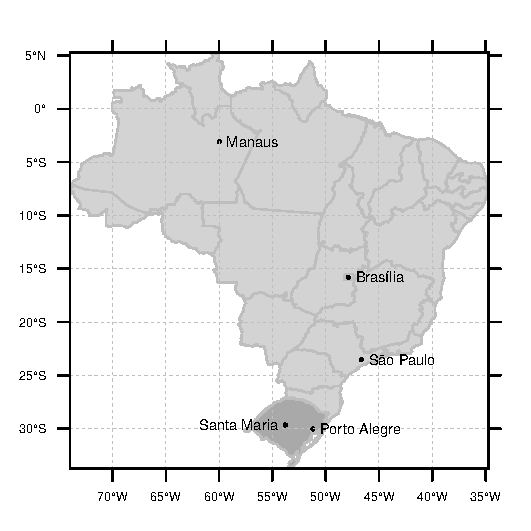
\includegraphics[width=90mm]{chap01FIG1a}
    \end{minipage}
    \begin{minipage}[b]{95mm}
      \subcaption{}
      \label{fig:points}
      \centering
      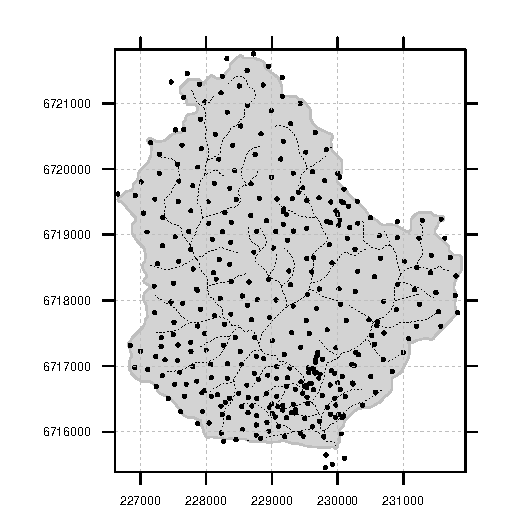
\includegraphics[width=90mm]{chap01FIG1b}
    \end{minipage}
  \caption{Location of the study area in Santa Maria (a) and spatial 
  distribution of the point soil observations and drainage network (b).}
  \label{fig:location}
 \end{figure}

A dataset containing $n=350$ point soil observations collected between 2004 and 2011 
\citep{PedronEtAl2006b, SamuelRosaEtAl2011a, MiguelEtAl2012, Samuel-RosaEtAl2013}
was used in this study (available at 
\url{https://github.com/samuel-rosa/dnos-sm-rs}). Sampling locations were 
selected purposively and by convenience \citep{Samuel-RosaEtAl2014b}. Three soil
pits were opened within an area of about 100~m$^2$ at most sampling locations to
obtain composite samples of the topsoil for laboratory analysis. Soil was 
collected to a depth of 20~cm or less when soil depth was smaller than 20~cm.
A few observations ($n=10$) correspond to individual samples collected up to 
30~cm. Sampling depth ranges from 2 to 30~cm, with a mean of 17.3~cm. We assumed
that the vertical, horizontal and temporal support differences between soil 
samples is negligible for the purpose of this study.

Three soil properties (fine earth fraction, $<2$~mm) were explored: clay content
(CLAY,~g~kg$^{-1}$), organic carbon content (SOC,~g~kg$^{-1}$), and effective 
cation exchange capacity (ECEC,~mmol~kg$^{-1}$). CLAY was determined by the 
pipette method. SOC was determined using wet digestion. ECEC was calculated as 
the sum of exchangeable bases plus exchangeable acidity. The soil properties 
selected were expected to present different patterns of spatial variation and 
correlation with the most dominant factors of soil formation \citep{Jenny1941} 
in the area: organisms (\textit{O}), relief (\textit{R}), and parent material 
(\textit{P}). CLAY was presumed to have a stronger relation with \textit{P}, 
while SOC was expected to be more correlated with \textit{O}. Because the soils 
of the study area were strongly eroded due to intense agriculture in the 20th 
century, both CLAY and SOC were also expected to be closely related with 
\textit{R}. Finally, ECEC was expected to be strongly correlated with \textit{P}
and \textit{O}, which is supported by its natural relationship with both CLAY 
and SOC.

 \begin{figure}[!ht]
   \centering
    \begin{minipage}[b]{63mm}
      \subcaption{}
      \centering
      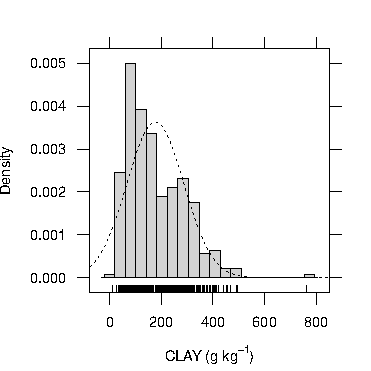
\includegraphics[width=63mm]{chap01FIG2a}
    \end{minipage}
    \begin{minipage}[b]{63mm}
      \subcaption{}
      \centering
      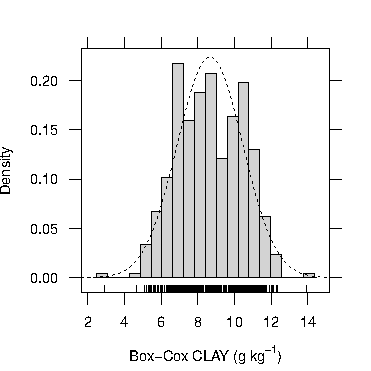
\includegraphics[width=63mm]{chap01FIG2d}
    \end{minipage}
    \begin{minipage}[b]{63mm}
      \subcaption{}
      \centering
      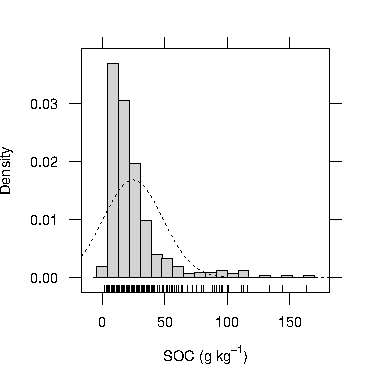
\includegraphics[width=63mm]{chap01FIG2b}
    \end{minipage}
    \begin{minipage}[b]{63mm}
      \subcaption{}
      \centering
      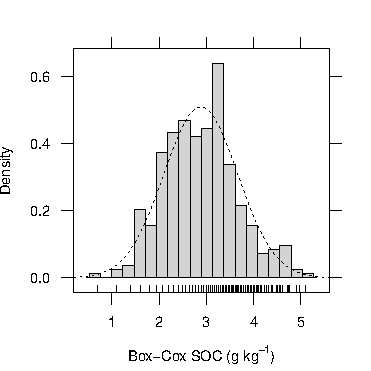
\includegraphics[width=63mm]{chap01FIG2e}
    \end{minipage}
    \begin{minipage}[b]{63mm}
      \subcaption{}
      \centering
      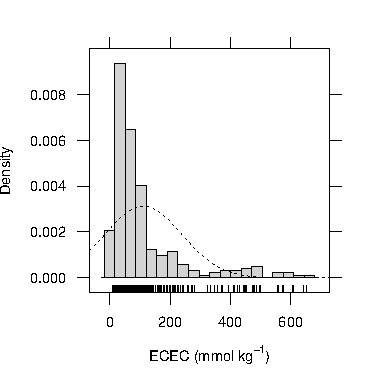
\includegraphics[width=63mm]{chap01FIG2c}
    \end{minipage}
    \begin{minipage}[b]{63mm}
      \subcaption{}
      \centering
      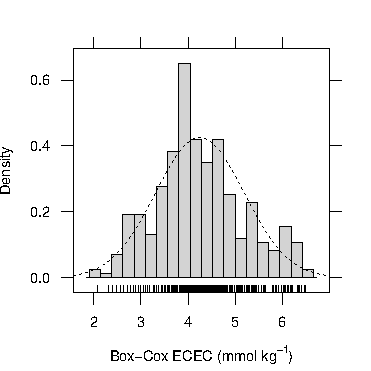
\includegraphics[width=63mm]{chap01FIG2f}
    \end{minipage}
  \caption{Histogram, empirical density function, and summary statistics of CLAY
  (a, b), SOC (c, d), and ECEC (e, f) in the original (left) and Box-Cox 
  feature spaces (right).}
  \label{fig:soil-properties}
 \end{figure}

Point soil data, here denoted by $Z(s)$, showed a positive skew 
(\autoref{fig:soil-properties}) and was normalized, $Z'(s)$, using the Box-Cox 
family of power transformations, where $Z'(s) = (Z(s)^{\lambda} - 1) / \lambda$,
if $\lambda > 0$, and $Z'(s) = log(Z(s))$, if $\lambda = 0$ 
\citep{DiggleEtAl2007}. Lambda ($\lambda$) values were selected empirically 
\citep{FoxEtAl2011}. Because the resulting distribution of the back-transform 
(see \autoref{subsec:validation}) has no expectation when $\lambda<0$ 
\citep{RibeiroEtAl2001}, a logarithm transformation ($\lambda=0$) was used when 
a negative $\lambda$ was estimated (SOC and ECEC).

\subsection{Environmental covariates}
\label{subsec:sources}

Five freely available environmental covariates were evaluated in this study, 
each with two levels of spatial detail: area-class soil maps (\texttt{soil}), 
geologic maps (\texttt{geo}), land use maps (\texttt{land}), digital elevation 
models (\texttt{dem}), and satellite images (\texttt{sat}). Each pair was 
composed by covariates that were produced separately from scratch using 
different data sources and/or production methods, thus demanding different 
amounts of resources (time, workforce, budget, technology, etc.). In this study,
the level of spatial detail of an environmental covariate is a function of the 
components of its production process such as the cartographic ratio 
(\texttt{soil}, \texttt{geo} and \texttt{land}), spatial sampling support 
(\texttt{sat}), number and diversity of data sources explored (\texttt{dem}),
and quantity of spatial data used (all five). Thus, the reader should bear in
mind that our definition of spatial detail is broader than spatial resolution
or spatial scale. It should also not be confounded with spatial support 
\citep{WebsterEtAl2007} or thematic detail \citep{Rossiter2000}.

The environmental covariates were transformed to predictor variables that were 
used in the geostatistical modelling. Since the transformation is different for
categorical and continuous covariates, the procedures are explained below for 
each type separately.

\subsubsection*{Categorical predictor variables}
\label{subsubsec:categorical-covars}

Area-class soil maps, geologic maps and land use maps are categorical 
environmental covariates (factors). Mapping units are the $k$ factor levels that
are transformed to as many dummy (indicator, binary) variables as there are 
factor levels, before model calibration. Each dummy variable receives a value 
equal to one (1) when a given class is present, and zero (0) otherwise 
\citep{Everitt2006}. If the number of point soil observations falling inside 
the spatial domain of a mapping unit is too small to accurately estimate a 
regression coefficient (we used a threshold of $n=15$ observations), the mapping
unit is merged with a similar mapping unit prior to calculating dummy variables.
The resulting generalized categorical covariate maps are shown in 
\autoref{fig:cat-covars}. The binary maps are the categorical predictor variables.

\noindent\textit{Soil maps}. The less detailed soil map (\soilOld) was published with a 
\scale{100,000} and has five mapping units \citep{AzolinEtAl1988} 
(\autoref{fig:soil-old}). It was produced using existing soil maps and technical
reports (\scale{750,000}) \citep{Brasil1973}, aerial photographs 
(\scale{60,000}), topographic maps (\scale{50,000}), and sparse point soil 
observations along the road network. The more detailed soil map (\soilNew) was 
prepared with a \scale{25,000} and has eight mapping units \citep{MiguelEtAl2012}
(\autoref{fig:soil-new}). It was produced using high spatial resolution satellite
images (65~cm), existing soil maps and technical reports published with a 
\scale{50,000} \citep{Poelking2007} and 1:25,000 \citep{PedronEtAl2006b}, 
topographic maps (\scale{25,000}), and descriptions from $\sim$~350 point soil 
observations. Five dummy predictor variables were derived from \soilOld{} and 
seven from \soilNew{} (\autoref{tab:soil-covars}).

 \begin{figure}[!ht]
    \centering
    \begin{minipage}[b]{63mm}
       \subcaption{Cartographic scale: 1:100,000}
       \label{fig:soil-old}
       \centering
       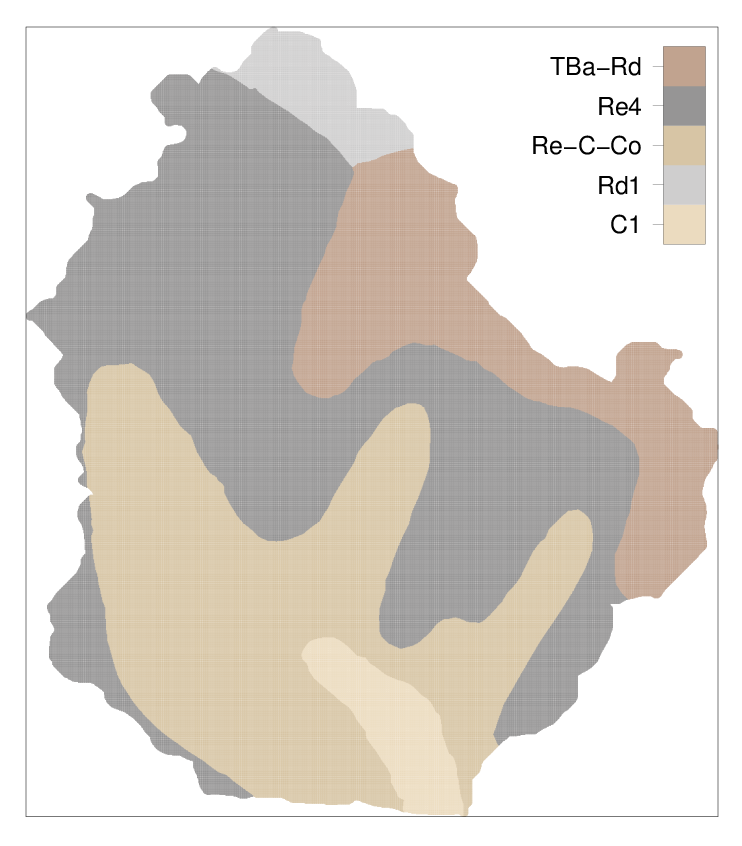
\includegraphics[width=60mm]{chap01FIG3a}
    \end{minipage}
    \begin{minipage}[b]{63mm}
       \subcaption{Cartographic scale: 1:25,000}
       \label{fig:soil-new}
       \centering
       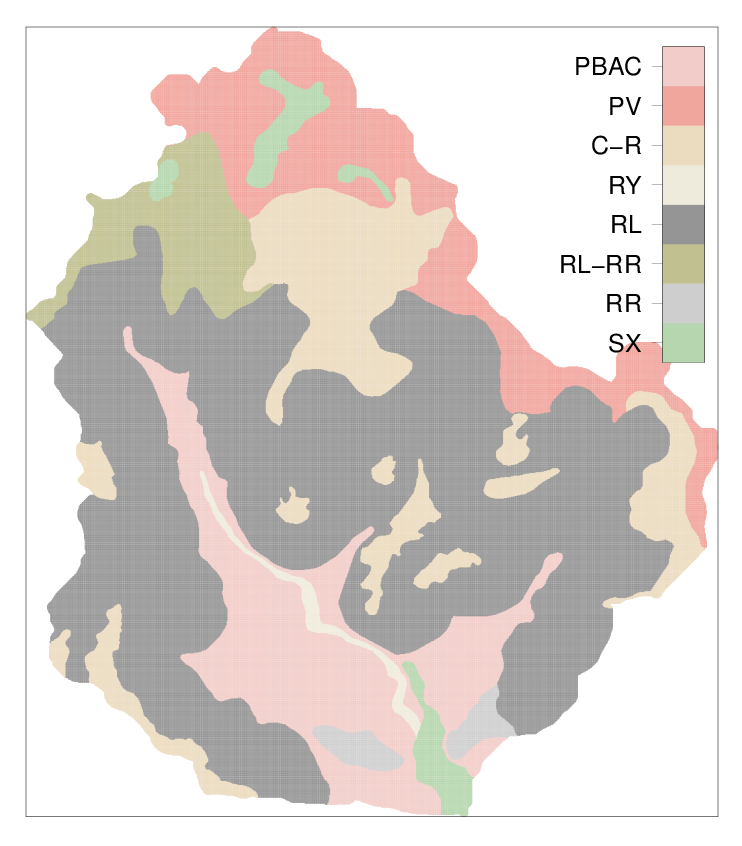
\includegraphics[width=60mm]{chap01FIG3d}
    \end{minipage}    
    \begin{minipage}[b]{63mm}
       \subcaption{Cartographic scale: 1:50,000}
       \label{fig:geo-old}
       \centering
       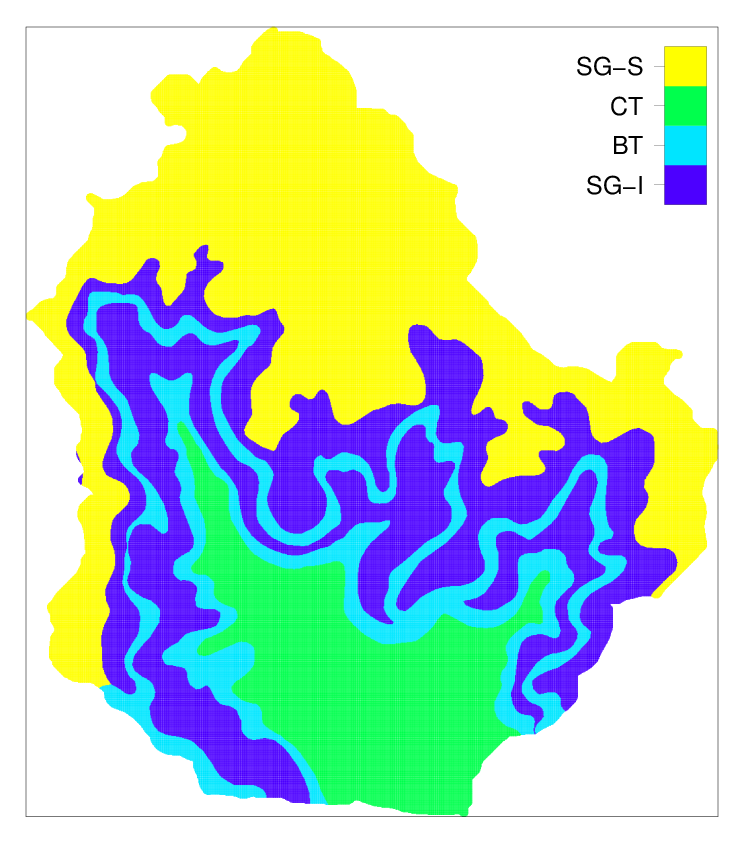
\includegraphics[width=60mm]{chap01FIG3b}
    \end{minipage}
    \begin{minipage}[b]{63mm}
       \subcaption{Cartographic scale: 1:25,000}
       \label{fig:geo-new}
       \centering
       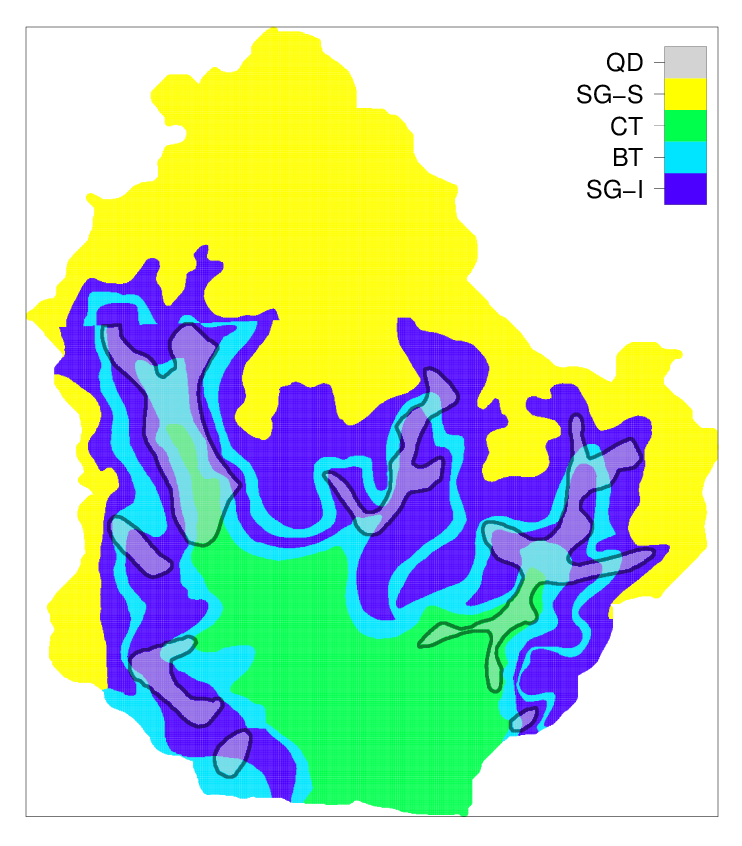
\includegraphics[width=60mm]{chap01FIG3e}
    \end{minipage}
    \begin{minipage}[b]{63mm}
       \subcaption{Cartographic scale: 1:500,000}
       \label{fig:land-old}
       \centering
       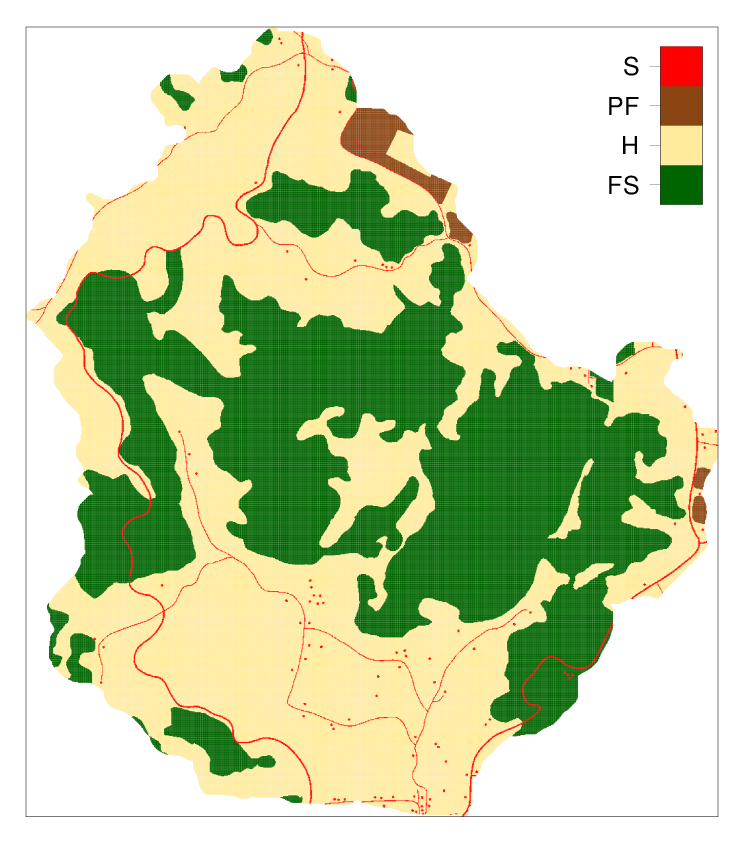
\includegraphics[width=60mm]{chap01FIG3c}
    \end{minipage}
    \begin{minipage}[b]{63mm}
       \subcaption{Cartographic scale: 1:2,000}
       \label{fig:land-new}
       \centering
       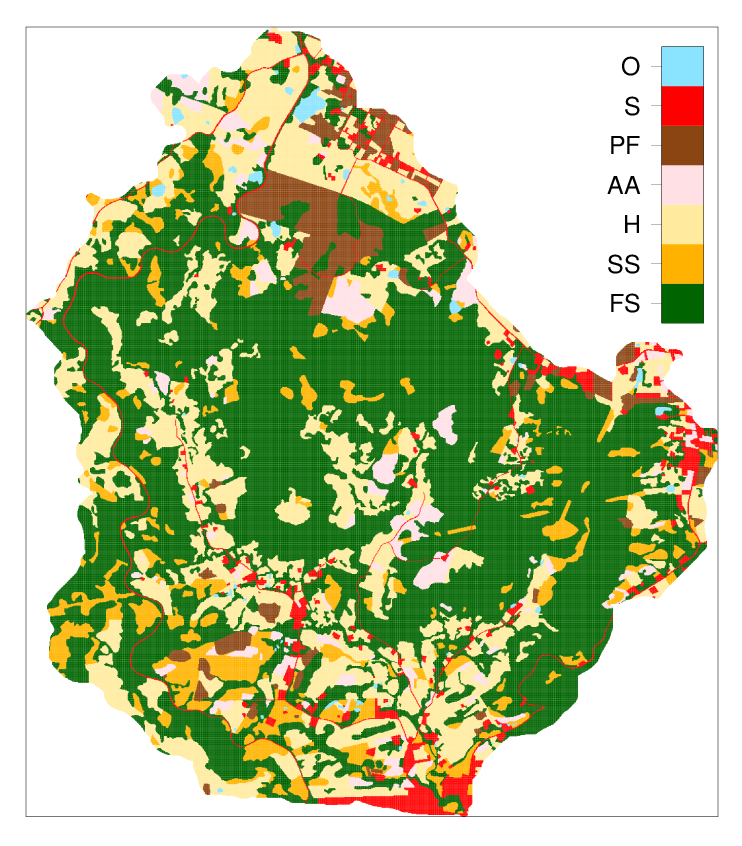
\includegraphics[width=60mm]{chap01FIG3f}
    \end{minipage}
   \caption{Area-class soil maps (a, b), geologic maps (c, d), and land use 
   maps (e, f) compared in our study. The less detailed version is displayed 
   at the left, while the more detailed version is shown on the right. Legend 
   abbreviations and derived dummy variables are described in Tables 
   \ref{tab:soil-covars}--\ref{tab:land-covars}.}
  \label{fig:cat-covars}
\end{figure}

\noindent\textit{Geologic maps}. The less detailed geologic map (\geoOld) was produced 
using topographic maps with \scale{50,000} \citep{GasparettoEtAl1988} 
(\autoref{fig:geo-old}). The more detailed geologic map (\geoNew) was produced 
using topographic maps with \scale{25,000}, and includes the location of 
overlaying Quaternary sedimentary deposits \citep{MacielFilho1990} 
(\autoref{fig:geo-new}). \geoNew{} did not cover a small part in the North of 
the study area, where \geoOld{} was used instead (this strategy was approved by
experts on the local geology). The mapping unit of both geologic maps depicting
the Caturrita Formation was used indirectly by deriving dummy predictor 
variables from all other individual mapping units. Three dummy predictor 
variables were derived from \geoOld{} and four from \geoNew{} 
(\autoref{tab:geology-covars}).

\noindent\textit{Land use maps}. The less detailed land use map (\landOld) was 
produced by manually digitizing land use data included in topographic maps with a 
\scale{25,000} \citep{DSG1980, DSG1992, DSG1992a} (\autoref{fig:land-old}). 
The more detailed land use map (\landNew) was prepared (\scale{2,000}) by 
manual digitization using 65~cm spatial resolution satellite images covering 
the years 2008 and 2009 \citep{SamuelRosaEtAl2011a} (\autoref{fig:land-new}). 
Mapping units depicting human settlements and water bodies ($n=0$) were not 
masked out from the prediction grid and were merged with other mapping units to
derive dummy predictor variables. Five dummy predictor variables were derived 
from \landNew{} and two from \landOld{} (\autoref{tab:land-covars}).

\subsubsection*{Continuous predictor variables}
\label{subsubsec:continuous-covars}

The less detailed DEM (\demOld) is the hole-filled SRTM DEM version~4 
\citep{JarvisEtAl2008} (\autoref{fig:dem-old}). The spatial sampling support of 
the SRTM DEM is 1~arc-second ($\sim$~30~m), but elevation data were aggregated 
to 3~arc-seconds ($\sim$~90~m) for public release in regions outside the United 
States \citep{ReuterEtAl2007}. The more detailed DEM (\demNew) was produced by 
interpolating contour lines with vertical spacing of 10~m along with data about 
the drainage network, lakes and peaks digitized from topographic maps with 
\scale{25,000} (\autoref{fig:dem-new}). Interpolation to 5-m pixel size was 
performed using a hydrologically correct algorithm implemented in \href{http://resources.arcgis.com/en/help/main/10.1/index.html#/How_Topo_to_Raster_works/009z0000007m000000/}{ArcGIS\textregistered{}} software by ESRI \citep{Hutchinson1989}. Contour line 
artefacts were minimized using a seven by seven low-pass filter 
(\grass{r.neighbors}). The window size was chosen such that the smoothed DEM 
best matched the original contour map while also respecting the original 
drainage network pattern.

\ctable[
   caption  = {Description of the $p=12$ dummy predictor variables derived from the two soil maps.},
   label    = tab:soil-covars,
   notespar,
   pos      = !ht,
%    doinside = \scriptsize\setstretch{1.1},
   doinside = \scriptsize
   ]{l p{0.85\textwidth} l}{
   \tnote[a]{Soil classification according to the old Brazilian classification (only for \citet{AzolinEtAl1988}), the current Brazilian classification \citep{SantosEtAl2013a}, and the international classification \citep{IUSSWorkingGroupWRB2007}.}
   \tnote[b]{Minimum Legible Delineation calculated following \citet{Rossiter2000}.}
   }{                                                                                                                    \FL
   Code                & Mapping unit(s) included and Description\tmark[a,b]                                             \ML
   \multicolumn{2}{l}{Source: \citet{AzolinEtAl1988}. Cartographic scale: 1:100,000. Minimum Legible Delineation: 40~ha.} \NN
   \texttt{SOIL\_100b} & \textit{Re4}. Shallow soils with low to high base saturation covering mountainous terrain (Solo Litólico Eutrófico/Distrófico relevo montanhoso; Neossolo Litólico Distrófico/Eutrófico; Distric/Eutric Leptosol). \NN 
   \texttt{SOIL\_100c} & \textit{Re-C-Co}. Shallow soils with high base saturation located in strongly sloping terrain (Solo Litólico Eutrófico relevo forte ondulado; Neossolo Litólico Eutrófico; Eutric Leptosol), low weathered soils (Cambissolo Eutrófico; Cambissolo Háplico Eutrófico; Eutric Cambisol), and colluvial deposits. \NN
   \texttt{SOIL\_100d} & \textit{TBa-Rd}. Deep, well-structured, low base saturation soils (Terra Bruna Estruturada álica; Nitossolo; Nitisol), and shallow soils (Solo Litólico; Neossolo Litólico; Leptosol). \NN
   \texttt{SOIL\_100e} & \textit{Rd1} and \textit{Re4}. \textit{Rd1} is composed mainly by shallow soils with low to high base saturation (Solo Litólico Distrófico/Eutrófico; Neossolo Litólico Distrófico/Eutrófico; Distric/Eutric Leptosol) located in slopping terrain. This dummy predictor variable is composed by shallow soils in both sloping and mountainous terrain. \NN
   \texttt{SOIL\_100f} & \textit{TBa-Rd} and \textit{C1}. \textit{C1} is composed by low weathered soils developed in lower landscape positions, close to drainage channels (Cambissolo Eutrófico; Cambissolo Eutrófico; Eutric Cambisol). This dummy predictor variable includes the best soil mapping units for crop agriculture among those identified in the soil survey. \NN
   &                                                                                                                     \NN
   \multicolumn{2}{l}{Source: \citet{MiguelEtAl2012}. Cartographic scale: 1:25,000. Minimum Legible Delineation: 2.5~ha.} \NN
   \texttt{SOIL\_25a}  & \textit{PBAC}. Moderately deep soils derived from sedimentary rocks, with abrupt textural change and low base saturation (Argissolo Bruno-Acinzentado; Alisol). \NN
   \texttt{SOIL\_25b}  & \textit{PV}. Deep soils derived from igneous rocks, with moderate textural gradient, and low base saturation (Argissolo Vermelho; Acrisol). \NN
   \texttt{SOIL\_25c}  & \textit{C-R}. Low weathered soils (Cambissolo; Cambisol) and shallow soils with low to high base saturation (Neossolo Litólico/Regolítico Eutrófico/Distrófico; Eutric/Distric Leptosol/Regosol). \NN
   \texttt{SOIL\_25d}  & \textit{RL}. Shallow soils with low to high base saturation (Neossolo Litólico Eutrófico/Distrófico; Eutric/Distric Leptosol). \NN
   \texttt{SOIL\_25h}  & \textit{PBAC}, \textit{PV} and \textit{SX}. \textit{SX} is composed by moderately deep soils derived from sedimentary rocks, with abrupt textural change, low base saturation, and which are saturated with water for long periods of the year (Planossolo Háplico; Planosol). This dummy predictor variable includes the best soil mapping units for crop agriculture among those identified in the soil survey. \NN
   \texttt{SOIL\_25i}  & \textit{RL}, \textit{RL-RR} and \textit{RR}. This dummy predictor variable includes all three mapping units composed mainly by shallow soils (Neossolo Litólico and Neossolo Regolítico; Leptosol and Regosol). \NN
   \texttt{SOIL\_25j}  & \textit{PV}, \textit{RL}, \textit{RL-RR} and \textit{C-R}. This dummy predictor variable includes all four mapping units composed mainly by soils derived from igneous rocks. \LL
   }

\ctable[
 caption  = {Description of the $p = 7$ dummy predictor variables derived from the two geologic maps.},
 label    = tab:chap05-geology-covars,
 notespar,
 pos      = !ht,
 % doinside = \scriptsize\setstretch{1.1}
 doinside = \scriptsize
 ]{l p{0.85\textwidth} l}{
 \tnote[a]{Minimum Legible Delineation calculated following \citeonline{Rossiter2000}.}
 }{ \FL
 Code & Mapping unit(s) included and Description\tmark[a] \ML
 \multicolumn{2}{l}{Source: \citeonline{GasparettoEtAl1988}. Cartographic scale: \num{1}:\num{50000}. Minimum 
 Legible Delineation: \SI{10}{\hectare}.} \NN
 \texttt{GEO\_50a} & \textit{SG-I}. Inferior Sequence of the Serra Geral Formation. Composed mainly of basic 
 igneous rocks (tholeiitic basalt and andesite). It is likely to be related with high CLAY and ECEC. \NN
 \texttt{GEO\_50b} & \textit{SG-S}. Superior Sequence of the Serra Geral Formation. Composed mainly of acid 
 igneous rocks (granophyric rhyolite and rhyodacite). It is likely to be related with moderate to high CLAY 
 and ECEC. \NN
 \texttt{GEO\_50c} & \textit{BT}. Botucatu Formation. Composed mainly of aeolian sandstones. It is likely to 
 be related with low CLAY and ECEC. \NN
 Other & \textit{CT} depicts the Caturrita Formation, which is composed mainly of fluvial sandstones. \NN
 & \NN
 \multicolumn{2}{l}{Source: \citeonline{MacielFilho1990}. Cartographic scale: \num{1}:\num{25000}. Minimum 
 Legible Delineation: \SI{2.5}{\hectare}.} \NN
 \texttt{GEO\_25a} & \textit{SG-I}. Inferior Sequence of the Serra Geral Formation. \NN
 \texttt{GEO\_25b} & \textit{SG-S}. Superior Sequence of the Serra Geral Formation. \NN
 \texttt{GEO\_25c} & \textit{BT}. Botucatu Formation. \NN
 \texttt{GEO\_25d} & \textit{QD}. Quaternary deposits of fluvial, alluvial, and colluvial origin. It can help 
 explaining the low CLAY of soils supposedly derived from igneous rocks. \NN
 Other & \textit{CT} depicts the Caturrita Formation. \LL
 }


\ctable[
   caption  = {Description of the $p=7$ dummy predictor variables derived from the two land use maps.},
   label    = tab:land-covars,
   notespar,
   pos      = !ht,
   %    doinside = \scriptsize\setstretch{1.1}
   doinside = \scriptsize
   ]{l p{0.85\textwidth} l}{
   \tnote[a]{Minimum Legible Delineation calculated following \citet{Rossiter2000}.}
   }{                                                                                                                                \FL
   Code             & Mapping unit(s) included and Description\tmark[a]                                                                       \ML
   \multicolumn{2}{l}{Source: \citet{DSG1980, DSG1992, DSG1992a}. Cartographic scale: 1:25,000. Minimum Legible Delineation: 2.5~ha.} \NN
   \texttt{LU1980a} & \textit{FS}. Native forest, which is likely to have soils with higher fertility.                              \NN
   \texttt{LU1980b} & \textit{H}. Animal husbandry, which is likely to have a soil fertility status lower than native forests and is the second most important land use in the area. \NN
   Other            & Plantation forests (\textit{PF}) and human settlements (\textit{S}).                                           \NN
    & \NN
   \multicolumn{2}{l}{Source: \citet{SamuelRosaEtAl2011a}. Cartographic scale: 1:2,000. Minimum Legible Delineation: 100~m$^2$.}      \NN
   \texttt{LU2009a} & \textit{FS}. Native forest.                                                                                    \NN
   \texttt{LU2009b} & \textit{SS}. Shrubland, which is likely to have SOC and ECEC level above those found in areas used with annual crop agriculture and animal husbandry, but lower than in native forests. \NN
   \texttt{LU2009c} & \textit{H}. Animal husbandry. \NN
   \texttt{LU2009d} & \textit{AA}. Annual crop agriculture, which is likely to have the lowest soil fertility due to the usually poor management practices employed. \NN
   \texttt{LUdiff}  & Land use difference between 1980 and 2009. It can be useful to explain, for example, low SOC in forest soils due to previous use with crop agriculture or animal husbandry. \NN
   Other            & Plantation forests (\textit{PF}), human settlements (\textit{S}), and other land uses (\textit{O}), comprising natural and artificial water bodies. \LL
   }


\begin{figure}[!ht]
  \centering
    \begin{minipage}[b]{63mm}
      \subcaption{Spatial resolution: 90~m}
      \label{fig:dem-old}
      \centering
      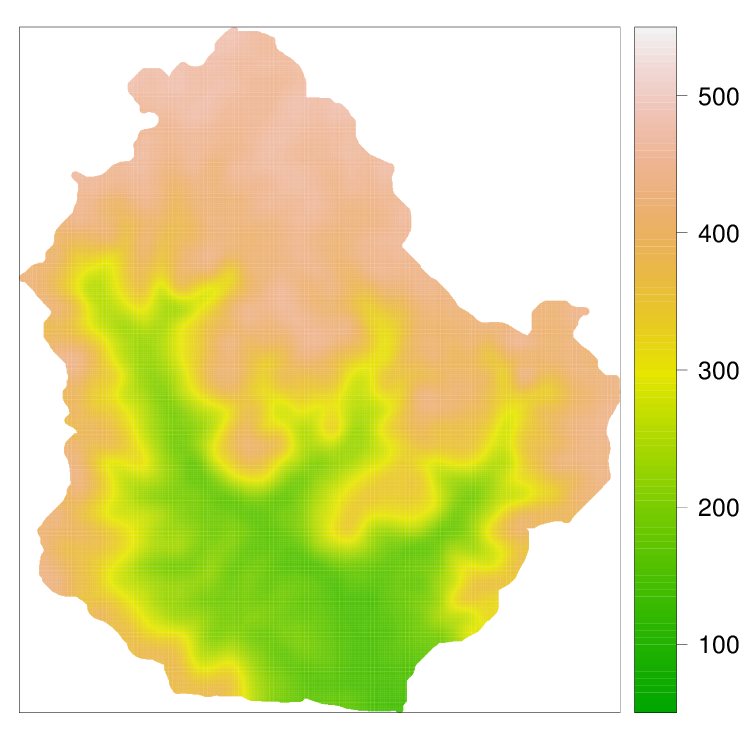
\includegraphics[width=60mm]{chap01FIG4a}
    \end{minipage}
    \begin{minipage}[b]{63mm}
      \subcaption{Spatial resolution: 30~m}
      \label{fig:sat-old}
      \centering
      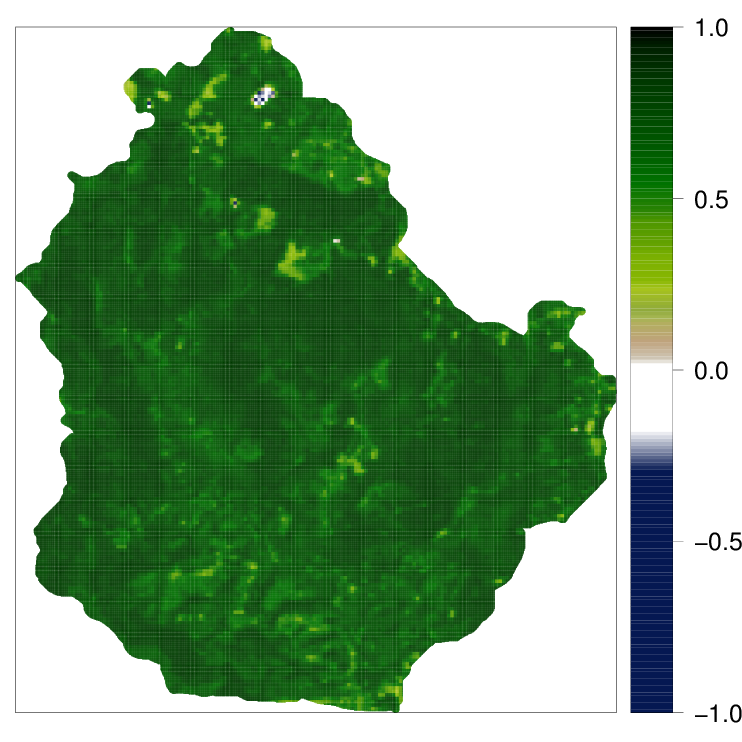
\includegraphics[width=60mm]{chap01FIG4b}
    \end{minipage}
    \begin{minipage}[b]{63mm}
      \subcaption{Vertical spacing of contours: 10~m}
      \label{fig:dem-new}
      \centering
      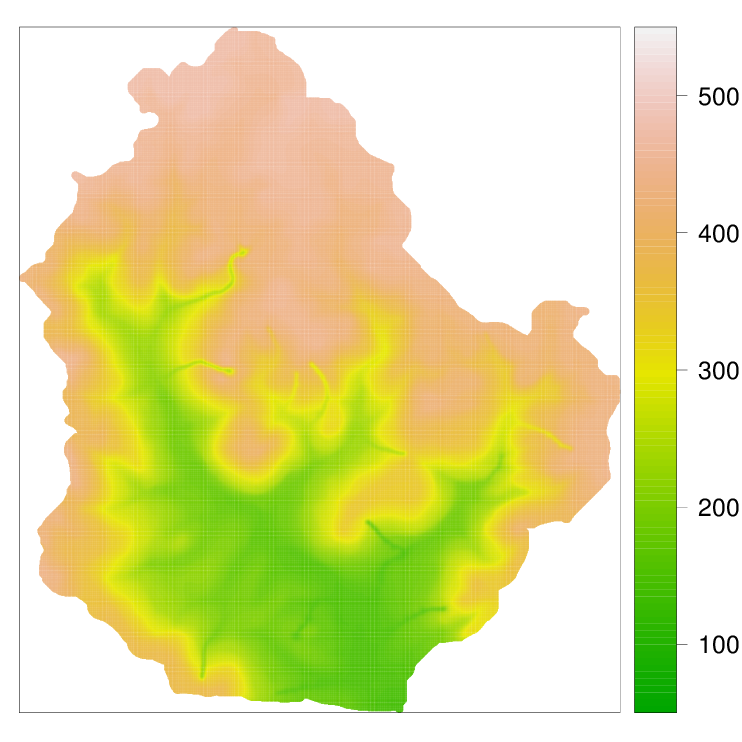
\includegraphics[width=60mm]{chap01FIG4c}
    \end{minipage}
    \begin{minipage}[b]{63mm}
      \subcaption{Spatial resolution: 5~m}
      \label{fig:sat-new}
      \centering
      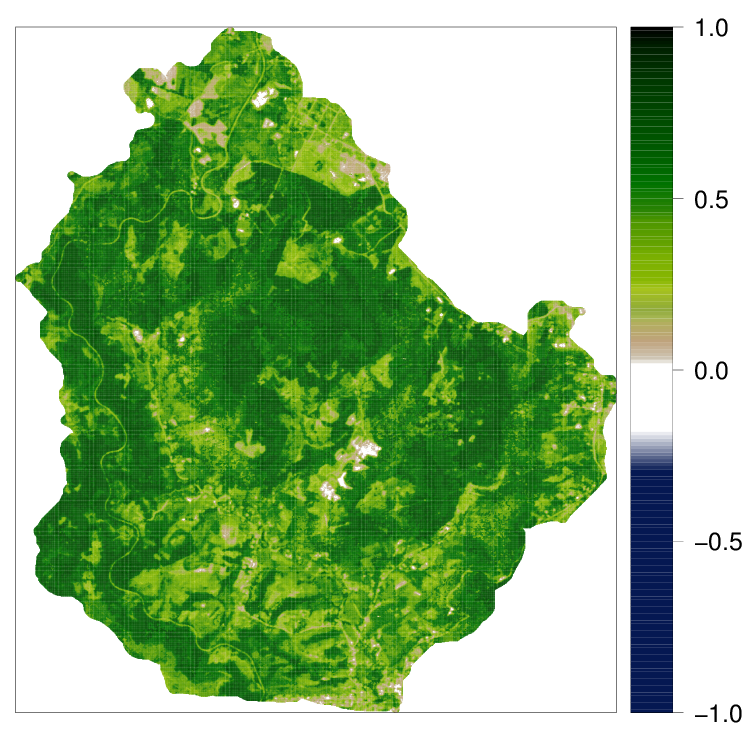
\includegraphics[width=60mm]{chap01FIG4d}
    \end{minipage}
  \caption{Digital elevation models (a, c) and satellite images, depicted using 
  the normalized difference vegetation index (b, d), compared in our study. The
  less detailed version is displayed at the top, while the more detailed version
  is shown on the bottom.}
  \label{fig:con-covars}
\end{figure}

Eight DEM derivatives were calculated: elevation (\elev), slope (\slp), aspect 
(\asp), northernness (\nor), flow accumulation (\acc), topographic wetness index
(\twi), stream power index (\spi), and topographic position index (\tpi). \slp{}
and \asp{} were calculated using \grass{r.param.scale} with seven window sizes 
(sampling support, analysis scale): 3, 7, 15, 31, 63, 127, and 255. \asp{} was 
scaled to the standard 0-360$^\circ$ range and orientation, and was transformed
to \nor{} using $\texttt{NOR} = abs(180^\circ - \texttt{ASP})$. \twi{} and \spi{}
were calculated using \slp{} calculated with different window sizes, and \acc{} 
calculated using \grass{r.watershed}. \tpi{} was calculated using 
\saga{ta\_morphometry} with the same seven window sizes. The combination of DEM
derivatives (\elev, \slp, \nor, \twi, \spi, and \tpi) and window sizes yielded 
$p=36$ continuous predictor variables from each DEM.

The less detailed satellite image was acquired by the Landsat-5 Thematic Mapper
on December 26, 2010 (available at Instituto Nacional de Pesquisas Espaciais - 
Divisão de Geração de Imagens -- \href{http://www.dgi.inpe.br/CDSR/}{INPE-DGI})
(\autoref{fig:sat-old}). It has 8~bits radiometric resolution and $\sim$~30~m 
spatial resolution. Spectral bands were orthorectified (Geomatica\textregistered{}
OrthoEngine\textregistered{}) and radiometrically corrected (\grass{i.landsat.toar}).
The more detailed satellite image comes from the RapidEye constellation 
(available at Ministério do Meio Ambiente -- 
\href{http://geocatalogo.ibama.gov.br/}{MMA}) (\autoref{fig:sat-new}). It was 
acquired on November 16, 2012, has 16~bits radiometric resolution, 6.5~m spatial
resolution, and was orthorectified to 5~m spatial resolution. Both images were 
atmospherically (6S atmospheric model \citep{VermoteEtAl1997}, \grass{i.atcorr})
and topographically corrected (\grass{i.topo.corr}). Derived predictor variables
are the spectral bands (except the thermal band) and vegetation indices 
(normalized difference vegetation index - NDVI, and soil-adjusted vegetation 
index - SAVI). Eight continuous predictor variables were derived from the 
Landsat-5~TM image and nine from the RapidEye image.

\subsubsection*{Additional processing}
\label{subsubsec:sources-processing}

Soil maps, geologic maps, land use maps, and satellite images were registered 
with the prediction grid (5-m pixel size) using nearest neighbour resampling. 
\demOld{} was registered using cubic resampling \citep{Samuel-RosaEtAl2013c}. 
Systematic positional errors were corrected using affine transformation 
\citep{Samuel-RosaEtAl2014}.

\subsection{Linear mixed model of spatial variation}
\label{subsec:lmm}

We model each of the soil properties of interest as the outcome of a spatial 
stochastic process. The model is composed of fixed and random effects 
\citep{HeuvelinkEtAl2001, LarkEtAl2006}. We use the point soil observations and 
spatially exhaustive predictor variables to calibrate the model and predict the
outcome of the spatial stochastic process at unobserved locations. This fixed 
effect (deterministic trend), $\mu(\textbf{s})$, describes that part of the 
spatial variation of the soil property that is explained by the covariates. We 
assume here that is a linear function of the predictor variables. The random 
effect (stochastic residuals, latent variables), $\varepsilon(\textbf{s})$, 
describes that part of the spatial variation that cannot be explained by the 
covariates \citep{Cressie1993}. It is represented by a spatially correlated, 
Gaussian distributed random variable, that is assumed stationary in the mean 
and covariance. Thus, the linear mixed model of spatial variation that we 
employed is given by

\begin{equation}\label{eq:lmm}
 Z'(\textbf{s}) = \mu(\textbf{s}) + \varepsilon(\textbf{s}) = \sum_{j=0}^{p} 
 \beta_{j}\cdot X_{j}(\textbf{s}) + \varepsilon(\textbf{s}),
\end{equation}

\noindent{where $Z'(\textbf{s})$ is the soil property after Box-Cox 
transformation, $\mu(\textbf{s})$ and $\varepsilon(\textbf{s})$ are defined as 
above, $\beta_{j}$ are the regression model coefficients, and $X_{j}(\textbf{s})$
is the regression model matrix, with $j=0, 1, 2, \ldots, p$, $p$ being the number
of predictor variables. Variable $X_{0}(\textbf{s})$ is taken as unity so that 
$\beta_{0}$ is the intercept.}

\subsubsection*{Model selection}

We calibrated $m=2^5=32$ multiple linear regression models for each soil property
(fitted using ordinary least squares, OLS) to model the deterministic trend for 
each combination of the five covariates (recall from \autoref{sec:intro} that 
each covariate is available at two levels of spatial detail, hence $2^5$ 
combinations). The number of predictor variables used to calibrate each model 
varied among combinations between $p=52$ and $p=62$, because more detailed 
covariates enabled the derivation of a larger number of predictor variables 
(except the DEM). Backward VIF (variance inflation factor) selection followed 
by stepwise AIC (Akaike's Information Criterion) selection were used to select 
predictor variables to enter the models \citep{Samuel-RosaEtAl2014c, VenablesEtAl2002}.

The $m=32$ multiple linear regression models calibrated for each soil property 
were ranked using the ratio between the regression sum of squares and the total 
sum of squares. Because stepwise regression results in biased models 
\citep{Harrell2001a}, the ratio of sum of squares was adjusted (${R}^{2}_{adj}$)
using the number of predictor variables initially offered to enter the model 
instead of the reduced number of predictor variables that entered the model. 
Next, the five environmental covariates were ranked based on how their level of 
spatial detail related with the calibration of models with improved predictive 
performance. The relation between the level of spatial detail of the covariates 
and model performance was evaluated using a graphical output called model series
plot (\Rpackage{pedometrics}, \citet{Samuel-RosaEtAl2014c}). Pedological 
evaluation of predictor variables included in the models was omitted because 
this was beyond our objectives.

The multiple linear regression model calibrated using only the less detailed 
environmental covariates, which we call the \textit{baseline} model, and the 
multiple linear regression model with the highest ${R}^{2}_{adj}$, which we call
the \textit{best performing} model, were extended to linear mixed models of 
spatial variation (\autoref{eq:lmm}) for each soil property. Estimation of the 
parameters of the linear mixed models was performed using residual (restricted,
marginal) maximum likelihood (REML) \citep{RibeiroEtAl2001, LarkEtAl2004}. The 
spatial correlation function adopted was the exponential function (this is 
equivalent to the Matérn correlation function with smoothness parameter 
$\nu=0.5$ \citep{Stein1999}).

\subsubsection*{Model validation}
\label{subsec:validation}

Only the \textit{baseline} and \textit{best performing} multiple linear 
regression and linear mixed models calibrated for each soil property were 
validated. Model validation was performed using leave-one-out cross-validation 
(LOO\-/CV) \citep{BrusEtAl2011}. All model parameters were re-estimated at each
LOO\-/CV run to reduce bias \citep{LaslettEtAl1987}. LOO\-/CV predicted values 
were back-transformed from the Box-Cox space to the original space of soil 
properties using stochastic simulation \citep{ChristensenEtAl2001}:

\begin{enumerate}
 \item each predicted value and associated prediction error variance were used 
 to simulate $n = 20,000$ values from a Gaussian distribution;
 \item simulated values were back-transformed using 
 $Z(s) = (Z'(s) \times \lambda + 1)^{1 / \lambda}$, if $\lambda > 0$, and 
 $Z(s) = exp(Z'(s))$, if $\lambda = 0$;
 \item the mean and variance of back-transformed simulated values were used as 
 the predicted value and prediction error variance in the original space of 
 soil properties.
\end{enumerate}

Five error statistics were computed from the LOO\-/CV results 
\citep{JanssenEtAl1995, KempenEtAl2010, BrusEtAl2011}. The mean error 
(\textit{ME}), which measures the prediction bias, the mean absolute error 
(\textit{MAE}) and the root mean squared error (\textit{RMSE}), which measure 
the prediction accuracy, the scaled root mean squared error (\textit{SRMSE}, 
also known as mean squared deviation ratio), which measures how well the 
prediction error variance matches the squared differences between predicted and 
observed soil property, where $\textit{SRMSE}>1$ indicates under-estimation, 
while $\textit{SRMSE}<1$ indicates over-estimation, and the amount of variance 
explained (\textit{AVE}, also known as coefficient of determination or ratio of
scatter), which measures the fraction of the overall spread of observed values 
that is explained by the model. The AVE ranges from 0 to 100, where 
$\textit{AVE}=100$ is the optimal value.

\subsubsection*{Spatial prediction}
\label{subsec:prediction}

Only the \textit{baseline} and \textit{best performing} linear mixed models 
calibrated for each soil property were used for spatial prediction. Spatial 
predictions at a fine grid of $\sim$~800,000 point locations were made in the 
Box-Cox space using the best linear unbiased predictor (BLUP) with the 
empirical estimates of the random effects (EBLUP) \citep{LarkEtAl2006}. EBLUP 
with a fixed effect model is conceptually equivalent to kriging with external 
drift and regression kriging, and mathematically equivalent to kriging with 
external drift and universal kriging. Point predicted values and prediction 
error variances were back-transformed to the original soil property space using
stochastic simulation as described above (\autoref{subsec:validation}).

\section{Results}
\label{sec:results}

\subsection{Model series plots}

The model series plot is a graphical description of the relation between the 
prediction accuracy of multiple linear regression models and the environmental 
covariates used to calibrate them (\autoref{fig:model-series}). The magnitude 
of improvement in prediction accuracy is depicted in the bottom panel by the 
${R}^{2}_{adj}$. The top panel is interpreted both horizontally and vertically.
In the vertical direction we identify which version of each covariate was used 
to calibrate a given model. The less and the more detailed versions are 
identified by the yellow (bright) and green (dark) colours, respectively. The 
\textit{baseline} model is identified by the column containing only yellow 
cells, while the column with only green cells represents the model calibrated 
using only the more detailed version of each covariate, which we call the 
\textit{most detailed} model. The first important results that we obtain from 
the model series plots is that a) the \textit{baseline} model is not the model
with the lowest ${R}^{2}_{adj}$, which we call the \textit{poorest performing} 
model, and b) the \textit{most detailed} model is not the \textit{best 
performing} model.

\begin{figure}[!ht]
  \centering
    \begin{minipage}[b]{\textwidth}
      \subcaption{}
      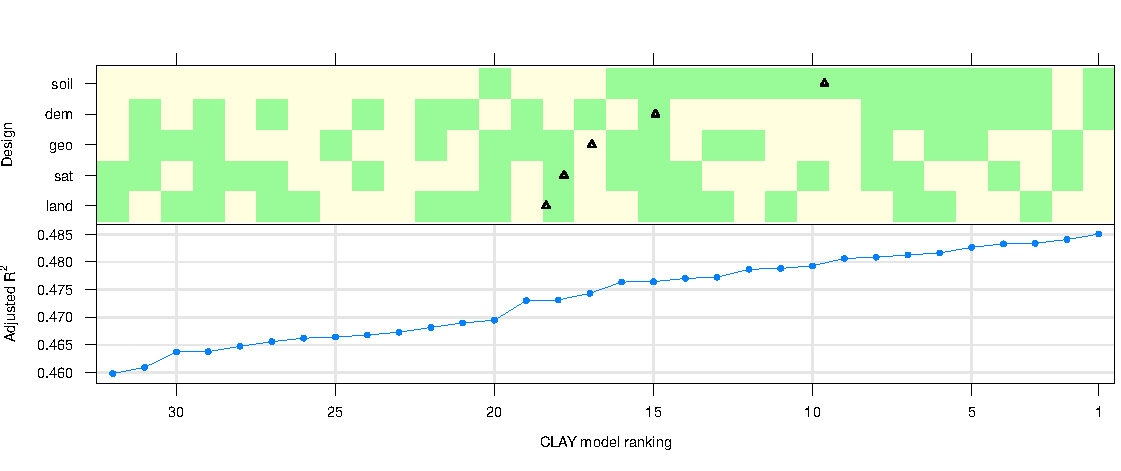
\includegraphics[width=\textwidth]{chap01FIG5a}
    \end{minipage}
    \begin{minipage}[b]{\textwidth}
      \subcaption{}
      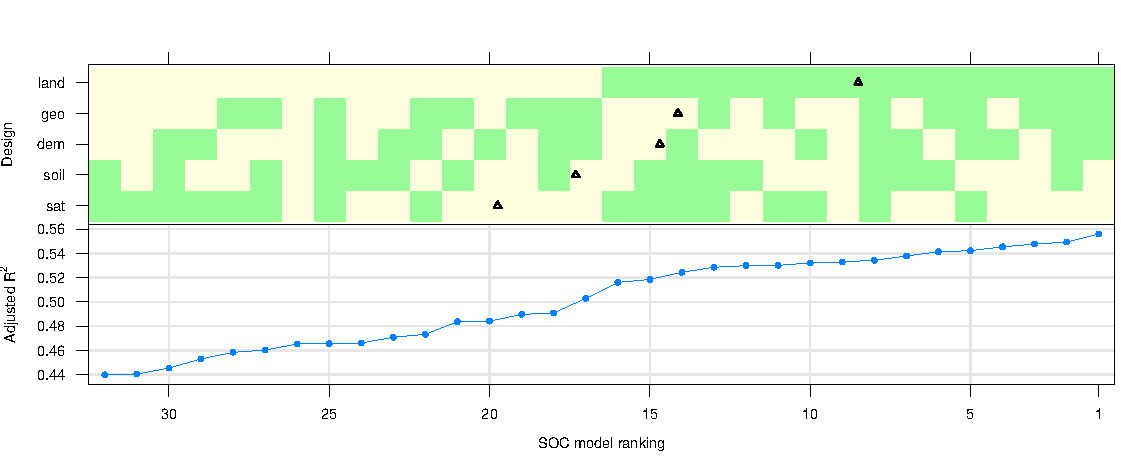
\includegraphics[width=\textwidth]{chap01FIG5b}
    \end{minipage}
    \begin{minipage}[b]{\textwidth}
      \subcaption{}
      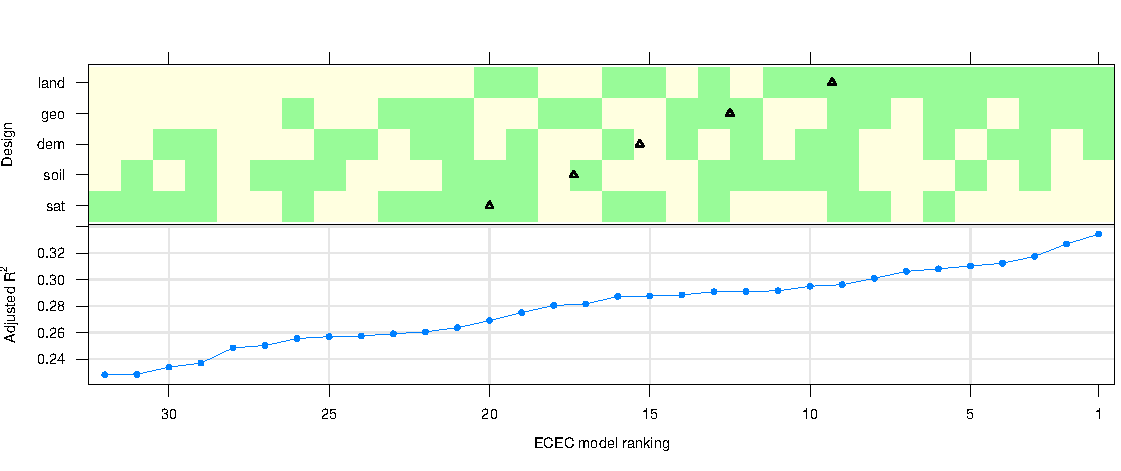
\includegraphics[width=\textwidth]{chap01FIG5c}
    \end{minipage}
  \caption{Model series plots for CLAY (a), SOC (b), and ECEC (c). The less and 
  more detailed version of each environmental covariate are identified by the 
  yellow (bright) and green (dark) colours, respectively. Multiple linear 
  regression models were ranked by their ${R}^{2}_{adj}$. Triangles show the 
  mean ranking of the more detailed covariates (i.e. centre of green cells).}
  \label{fig:model-series}
\end{figure}

The row-wise analysis of the model series plots shows if a model calibrated with
the more detailed version of a given environmental covariate has a higher 
prediction accuracy. This information is retrieved by looking at the row-wise 
distribution of green cells -- these cells represent the $m=16$ models 
calibrated using the more detailed version of a given covariate, irrespective 
of the version of the other covariates. The more concentrated the green cells 
are in the right half of the plot, the larger the relative benefit of using the
more detailed version of that environmental covariate. For example, the top row
of the second model series plot shows the SOC models calibrated using the two 
versions of the land use map (\texttt{land}). All green cells are on the right
half of the plot between rankings 1 and 16 (see the x axis). The four lower rows
show that the green cells of the other four covariates are distributed along the
entire ranking range (from 1 to 32). This means that the relative benefit of 
calibrating a SOC model with a more detailed land use map is larger compared to 
that of using a more detailed version of the other covariates.

The centre of the row-wise distribution of the green cells for each 
environmental covariate, calculated as the mean ranking, is represented by the 
triangles. The mean ranking quantifies the relative benefit of using a more 
detailed version of each covariate. For example, the mean ranking of the SOC 
models calibrated using the more detailed land use map is about 8 (top row), 
while the mean ranking of the models calibrated using the more detailed 
satellite image (\texttt{sat}) is close to 20 (bottom row). Using the more 
detailed DEM (\texttt{dem}) is almost as beneficial as using the more detailed 
geologic map (\texttt{geo}) -- the mean ranking of the SOC models calibrated 
using the more detailed version of these two covariates is about 15-16 (second 
and third rows). Using the more detailed version of the soil map (\texttt{soil},
fourth row) is not as beneficial as using \texttt{land}, \texttt{geo} or 
\texttt{dem}, but more beneficial than using \texttt{sat}. Because the 
covariates were ranked based on the mean rankings, the covariate displayed in 
the top row of each model series plot is the one which resulted in the largest
improvement of the prediction accuracy when the more detailed version was used 
to calibrate the model -- for SOC this is the land use map.

For CLAY, calibrating the models with the more detailed soil map resulted in 
the largest improvement of the prediction accuracy relative to the other 
environmental covariates. The DEM was the second most beneficial covariate (mean
ranking of 15), but the benefit of using its more detailed version was similar 
to that of using the more detailed version of any other covariate (mean rankings
between 17 and 18). Nine models had a poorer prediction performance than the 
baseline model, ranked 27th, the poorest performing model being that calibrated 
with the more detailed land use map and satellite image. Despite these patterns,
calibrating CLAY models with the more detailed version of any covariate resulted
in a small improvement of the prediction accuracy, as evidenced by the small 
increases of the ${R}^{2}_{adj}$. The difference between the poorest and best
performing models is less than 3~percentage points (pp). In comparison, for 
SOC, by simply using the more detailed land use map we already obtained a model
ranked 9th, an increase of 8~pp in ${R}^{2}_{adj}$ compared to the baseline 
model, ranked 24th.

The same general pattern observed for SOC models was observed for ECEC models -- 
the more detailed land use map results in the largest improvement of the 
prediction accuracy. The main difference is that calibrating the models with 
the more detailed geologic map was slightly more beneficial for ECEC (mean 
ranking of 12) than for SOC (mean ranking of 14). The poorest performing ECEC 
model was that calibrated with the more detailed satellite image. Using only 
the more detailed land use map resulted in an improvement of 6~pp in 
${R}^{2}_{adj}$ (model ranked 7th), differing from the best performing model by 
only 2~pp. Using the more detailed version of all environmental covariates 
except the soil map or satellite image resulted in increases of about 6 and 
7~pp in ${R}^{2}_{adj}$, respectively. The baseline model was ranked as 28th, 
which is a higher ranking than the models calibrated with all possible 
combinations of the more detailed satellite image and the more detailed
soil map and/or DEM.

The patterns observed in the model series plots resulted from the change 
(increase or decrease) of the importance of each environmental covariate on 
explaining the variance when the more detailed version was used 
(\autoref{tab:drop}). We used the \textit{baseline} and \textit{most detailed} 
models to quantify this change. Each model was refitted dropping one covariate 
at a time. The difference $\Delta$ between the ${R}^{2}_{adj}$ of the model 
calibrated with all five $q$ covariates (${R}^{2}_{adj}{}_{q=5}$) and the model 
calibrated without the $q$-th covariate ($R^{2}_{adj}{}_{q=5-1}$) was calculated.
The more positive $\Delta{R}^{2}_{adj}$ becomes, the more beneficial the more 
detailed version of the $q$-th covariate is for improving prediction accuracy.
For CLAY, \texttt{dem} and \texttt{land} were the most important covariates in 
the baseline model, while \texttt{geo} was the least important. The importance 
of \texttt{soil} and \texttt{geo} increased when their more detailed version 
was used (change of $+0.013$~pp for both), while \texttt{sat}, \texttt{land} 
and \texttt{dem} became less important. For SOC and ECEC, \texttt{land} was not 
the most important covariate in the baseline model. But it was the covariate 
whose importance had the largest positive shift when the more detailed version 
was used ($+0.085$~pp for SOC and $+0.045$~pp for ECEC). \texttt{sat} became 
less important when the more detailed version was used -- see its low ranking
in all model series plots. The increase of the importance of \texttt{geo} was 
larger for ECEC ($+0.026$) than for SOC ($+0.013$) -- see the difference in the 
mean ranking of \texttt{geo} in the SOC (14) and ECEC (12) model series plots.

\ctable[
   caption  = {The importance of each environmental covariate$^a$ ($\Delta{R}^{2}_{adj}{}^b$) in the models calibrated with their less and more spatially detailed version.},
   label    = tab:drop,
   pos      = !h,
   %    doinside = \scriptsize\setstretch{1.1}
   doinside = \scriptsize
   ]{lrrcrrcrr}{
   \tnote[a]{Covariate: \texttt{soil} - soil map, \texttt{land} - land use map, \texttt{geo} - geologic map, \texttt{sat} - satellite image, and \texttt{dem} - digital elevation model.}
   \tnote[b]{$\Delta{R}^{2}_{adj} = {R}^{2}_{adj}{}_{q=5} - R^{2}_{adj}{}_{q=5-1}$, where $q$ is the number of covariates included in the model. Negative values result from adjusting the $R^{2}$ using the number of predictor variables initially offered to enter the model instead of the reduced number of predictor variables that entered the model.}
   }{\FL
   \multicolumn{1}{l}{Covariate}&\multicolumn{2}{c}{CLAY}&\multicolumn{1}{c}{}&\multicolumn{2}{c}{SOC}&\multicolumn{1}{c}{}&\multicolumn{2}{c}{ECEC}\NN
   \cline{2-3} \cline{5-6} \cline{8-9}
   \multicolumn{1}{l}{}&\multicolumn{1}{c}{Less}&\multicolumn{1}{c}{More}&\multicolumn{1}{c}{}&\multicolumn{1}{c}{Less}&\multicolumn{1}{c}{More}&\multicolumn{1}{c}{}&\multicolumn{1}{c}{Less}&\multicolumn{1}{c}{More}\ML
   \texttt{soil} &$-0.009$&$ 0.004$&&$-0.006$&$-0.008$&&$ 0.011$&$-0.003$\NN
   \texttt{land} &$ 0.003$&$-0.002$&&$ 0.003$&$ 0.088$&&$-0.004$&$ 0.041$\NN
   \texttt{geo}  &$-0.019$&$-0.006$&&$-0.005$&$ 0.008$&&$ 0.007$&$ 0.033$\NN
   \texttt{sat}  &$-0.010$&$-0.016$&&$ 0.018$&$-0.014$&&$ 0.011$&$-0.029$\NN
   \texttt{dem}  &$ 0.030$&$ 0.001$&&$-0.009$&$ 0.016$&&$-0.035$&$-0.041$\LL
}

\subsection{REML fit of the variogram model}

The small improvement in the prediction accuracy of the CLAY linear mixed model 
calibrated with the more detailed environmental covariates is evidenced by 
\autoref{fig:lmm}. The shape of the experimental variogram is very similar 
for both baseline and best performing linear mixed models, which is also true 
for SOC and ECEC. However, the sill variance had a very small reduction for 
CLAY compared to SOC and ECEC. The last two showed a more considerable 
improvement in prediction accuracy. It can also be seen that the number of 
point observations separated by short distances is very small, reducing the 
accuracy of the estimate of the nugget variance. The result is that the 
estimated nugget variance changes rather erratically from the baseline to the 
best performing models, decreasing for CLAY and SOC, and increasing for ECEC.

\begin{figure}[!ht]
  \begin{center}
    \begin{minipage}[b]{90mm}
      \subcaption{}
      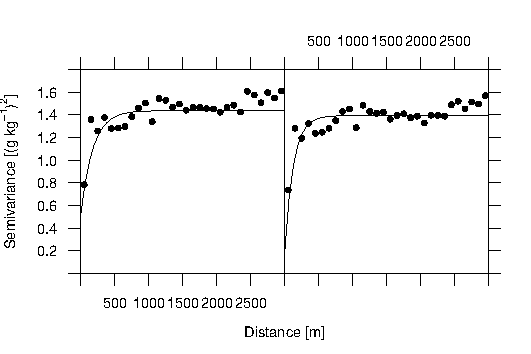
\includegraphics[width=90mm]{chap01FIG6a} 
    \end{minipage}
    \begin{minipage}[b]{90mm}
      \subcaption{}
      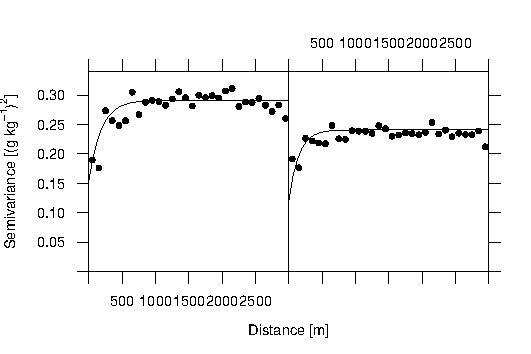
\includegraphics[width=90mm]{chap01FIG6b}
    \end{minipage}
    \begin{minipage}[b]{90mm}
      \subcaption{}
      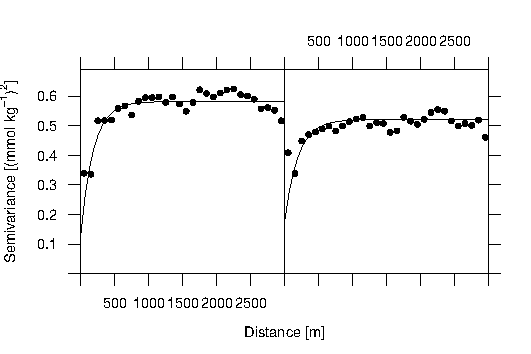
\includegraphics[width=90mm]{chap01FIG6c}
    \end{minipage}
    \caption{Experimental variogram (dots) and REML fit of the linear mixed 
    models (line) for CLAY (a), SOC (b), and ECEC (c). Left -- baseline model.
    Right -- best performing model.}
    \label{fig:lmm}
  \end{center}
\end{figure}

\subsection{Validation}

The LOO\-/CV results indicate that the linear mixed models for CLAY are slightly
positively biased, while those for SOC and ECEC are slightly negatively biased 
(\autoref{tab:cv-stats}). For both CLAY and ECEC, the \textit{MAE} shows that 
these models are more accurate than the multiple linear regression models, 
suggesting that the kriging step improves the prediction accuracy.

\ctable[
 caption = [Cross-validation of baseline and best performing models.]{Statistics$^a$ of the LOO\-/CV of 
baseline and best performing multiple linear regression models (LM) and linear mixed models (LMM).},
 label   = tab:chap05-cv-stats,
 notespar,
 pos = !th,
 % doinside = \scriptsize\setstretch{1.1}
 doinside = \small
 ]{llrrrrr}{
 \tnote[a]{Statistics: mean error (\textit{ME}), mean absolute error (\textit{MAE}), root mean squared error 
 (\textit{RMSE}), scaled root mean squared error (\textit{SRMSE}, unitless), and amount of variance explained 
 (\textit{AVE}, percent).}
 }{\FL
   \multicolumn{1}{l}{Model}&\multicolumn{1}{c}{Type}&\multicolumn{1}{c}{\textit{ME}}&\multicolumn{1}{c}{\textit{MAE}}&\multicolumn{1}{c}{\textit{RMSE}}&\multicolumn{1}{c}{\textit{SRMSE}}&\multicolumn{1}{c}{\textit{AVE}}\ML
   \multicolumn{7}{l}{CLAY (g kg$^{-1}$)}\NN
   ~~Baseline&LM&$ 1.31$&$52.1$&$ 72.1$&$0.89$&$56.8$\NN
   ~~&LMM&$ 0.94$&$48.5$&$ 68.8$&$1.03$&$60.7$\NN
   ~~Best performing&LM&$ 1.59$&$51.3$&$ 70.7$&$0.91$&$58.4$\NN
   ~~&LMM&$ 1.08$&$47.8$&$ 68.1$&$1.03$&$61.5$\ML
   \multicolumn{7}{l}{SOC (g kg$^{-1}$)}\NN
   ~~Baseline&LM&$-0.30$&$10.9$&$ 18.9$&$1.22$&$35.8$\NN
   ~~&LMM&$-0.39$&$11.0$&$ 19.4$&$1.43$&$32.5$\NN
   ~~Best performing&LM&$-0.20$&$10.1$&$ 16.9$&$0.91$&$49.0$\NN
   ~~&LMM&$-0.25$&$10.4$&$ 17.6$&$1.16$&$44.3$\ML
   \multicolumn{7}{l}{ECEC (mmol kg$^{-1}$)}\NN
   ~~Baseline&LM&$-0.88$&$70.6$&$112.4$&$0.97$&$22.3$\NN
   ~~&LMM&$-0.32$&$63.3$&$101.1$&$1.32$&$37.1$\NN
   ~~Best performing&LM&$-0.76$&$64.9$&$101.7$&$0.86$&$36.3$\NN
   ~~&LMM&$-0.29$&$62.6$&$ 97.9$&$1.09$&$41.1$\LL
}


Overall, all models had a moderate to poor prediction performance. The errors 
are, in absolute values, somewhat large, mainly for ECEC. The best \textit{AVE}
are about 60\% for CLAY, 50\% for SOC and 40\% for ECEC. In general, the 
prediction error variance was under-estimated by the linear mixed models and 
over-estimated by the multiple regression models. The best estimates of the 
prediction error variance were obtained by both CLAY linear mixed models, and 
the ECEC baseline linear regression model.

For CLAY, the increase in the \textit{AVE} was larger when including a kriging
step ($\Delta\textit{AVE}=3.9$~pp) than when using more detailed environmental
covariates ($\Delta\textit{AVE}=1.6$~pp). In the case of SOC, including a 
kriging step reduced the \textit{AVE} by 3.2~pp, and for ECEC, both strategies 
increased the \textit{AVE} (\autoref{tab:cv-stats}).

\subsection{Spatial prediction}

Both baseline and best performing linear mixed models captured the same overall
pattern of spatial variation of the soil properties (\autoref{fig:kriging}). 
The main difference is that the spatial patterns of the different environmental
covariates used to calibrate each model produced different features in the 
prediction maps. For example, the CLAY map produced by the best performing 
model (\autoref{fig:clay-best-pred}) displays abrupt changes in the predicted
values in the north-northeast due to the use of the more detailed soil map. 
Strongly-marked features following the stream network obtained through the use 
of the more detailed DEM are also observed (Figures \ref{fig:clay-best-pred} 
and \ref{fig:clay-best-var}).

SOC maps (Figures \ref{fig:soc-best-pred} and \ref{fig:soc-best-var}) show 
peculiar features in the central part of the study area, where predictions 
reached values as high as 507~g~kg$^{-1}$, while the maximum value in the 
calibration data is 163~g~kg$^{-1}$. The extremely high predicted values 
resulted from the inclusion of the topographic position index derived from 
the more detailed DEM, using a window size of 15~x~15~pixels 
(\texttt{TPI\_10\_15}) to model the deterministic trend. \texttt{TPI\_10\_15} 
values in the point calibration data range from -7 to 6~m, while in the central
part of the study area they range from 12 to 31~m. Thus, feature-space 
extrapolation explains the extremely high predicted values for SOC. Abrupt 
changes in predicted SOC are also observed at locations with low to moderate 
SOC (40 to 80~g~kg$^{-1}$). This is caused by using the more detailed land use 
map.

Predicted ECEC (Figures \ref{fig:ecec-base-pred} and \ref{fig:ecec-best-pred}) 
had a large dependency on land use and geologic maps. Several features observed
in the prediction maps derive from these two covariates. The influence of land 
use is seen in the northern part, while in the western, central, and eastern 
parts the influence of both covariates create an irregular pattern in the 
spatial distribution of ECEC. It is also in these parts that the largest 
prediction error standard deviations occur, following the spatial pattern of 
the covariates.

 \begin{figure}[!ht]
    \centering
    \begin{minipage}[b]{63mm}
      \subcaption{}
      \label{fig:clay-base-pred}
      \centering
      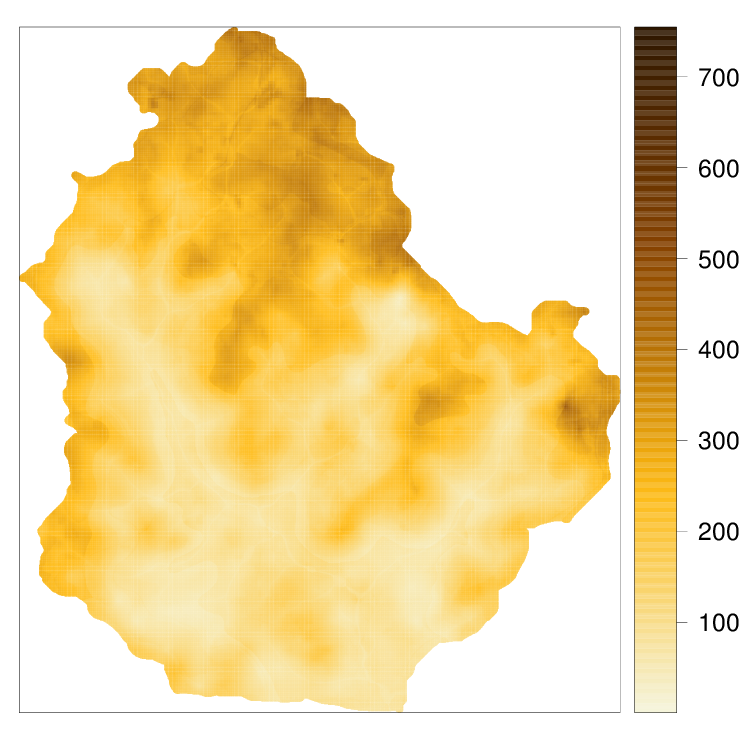
\includegraphics[width=63mm]{chap01FIG7a}
    \end{minipage}
    \begin{minipage}[b]{63mm}
      \subcaption{}
      \label{fig:clay-best-pred}
      \centering
      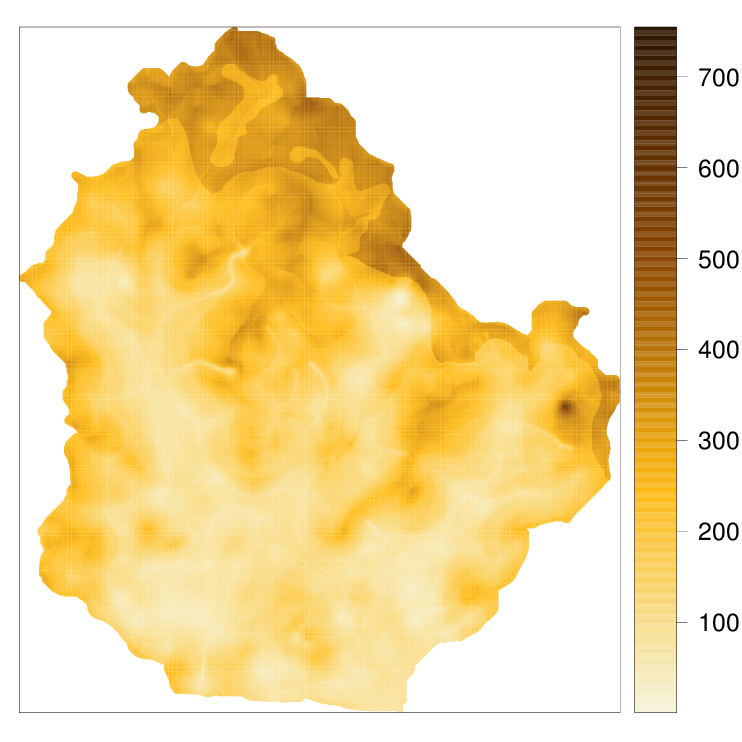
\includegraphics[width=63mm]{chap01FIG7d}
    \end{minipage}
    \begin{minipage}[b]{63mm}
      \subcaption{}
      \label{fig:soc-base-pred}
      \centering
      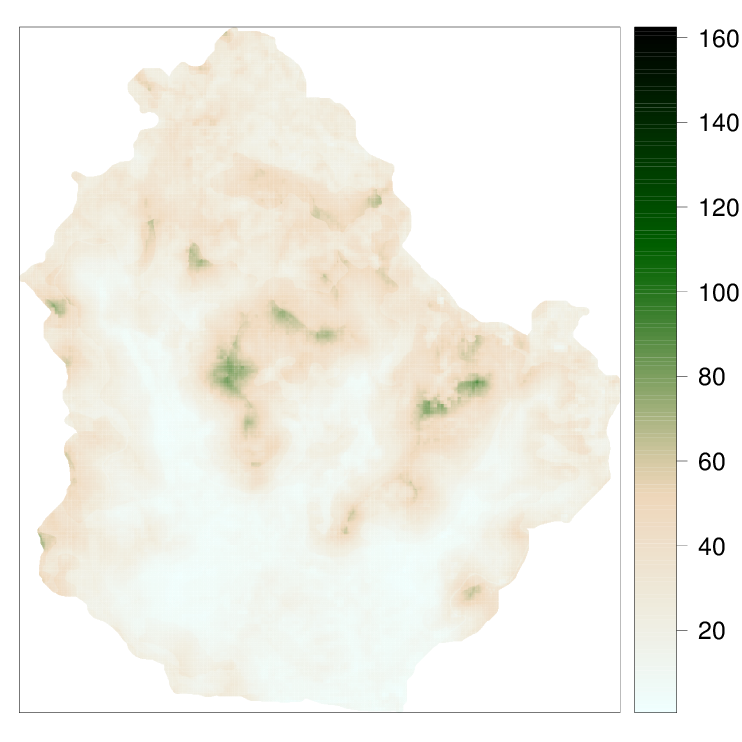
\includegraphics[width=63mm]{chap01FIG7b}
    \end{minipage}
    \begin{minipage}[b]{63mm}
      \subcaption{}
      \label{fig:soc-best-pred}
      \centering
      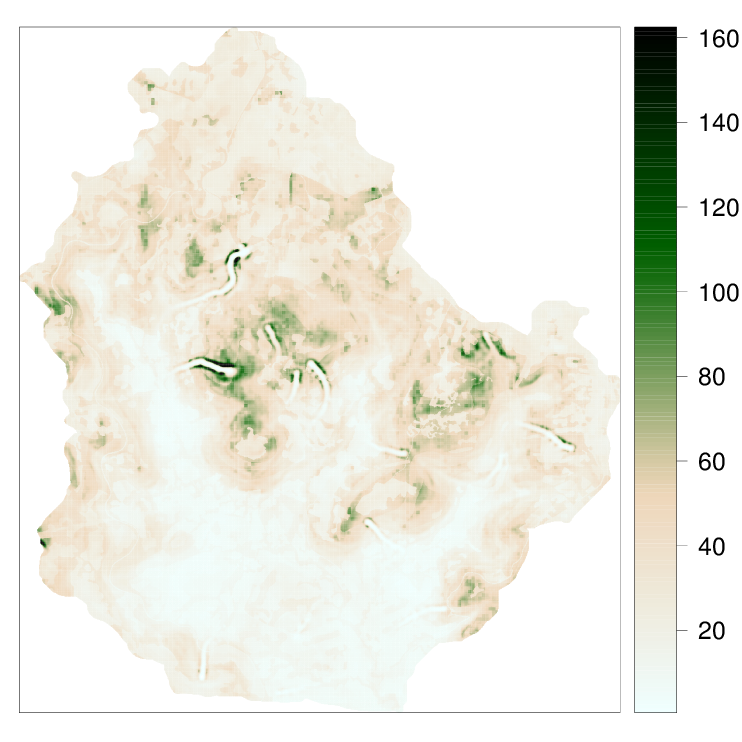
\includegraphics[width=63mm]{chap01FIG7e}
    \end{minipage}
    \begin{minipage}[b]{63mm}
      \subcaption{}
      \label{fig:ecec-base-pred}
      \centering
      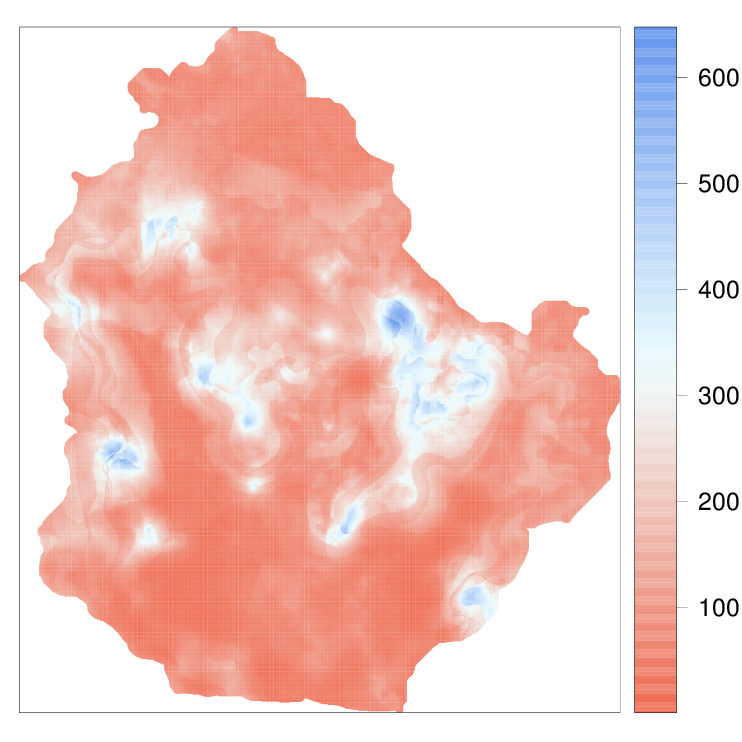
\includegraphics[width=63mm]{chap01FIG7c}
    \end{minipage}
    \begin{minipage}[b]{63mm}
      \subcaption{}
      \label{fig:ecec-best-pred}
      \centering
      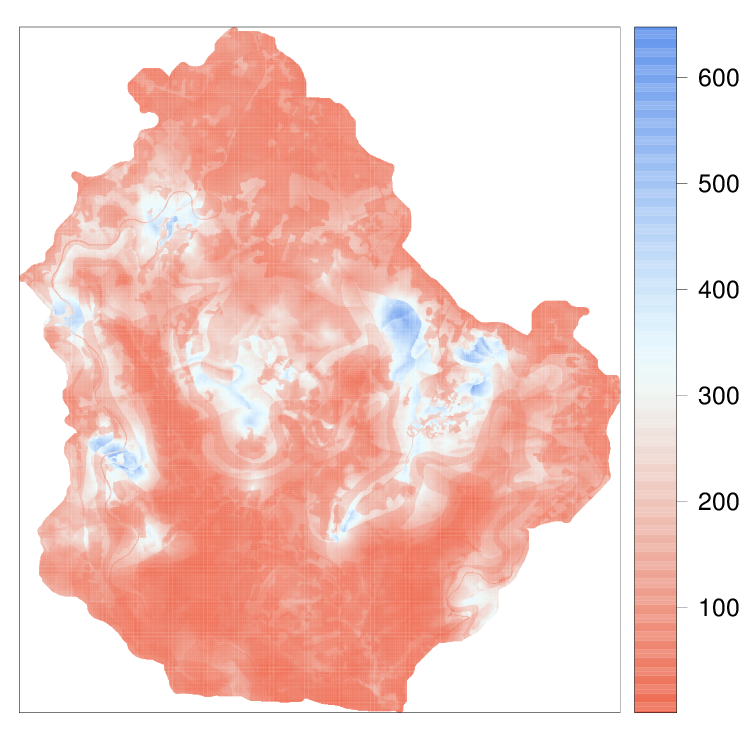
\includegraphics[width=63mm]{chap01FIG7f}
    \end{minipage}
  \caption{Predicted values for CLAY (g~kg$^{-1}$) (a, b), SOC (g~kg$^{-1}$) 
  (c, d), and ECEC (mmol~kg$^{-1}$) (e, f) using the baseline (left) and best 
  performing (right) linear mixed models.}
  \label{fig:kriging}
\end{figure}

\begin{figure}[!ht]
\centering
    \begin{minipage}[b]{63mm}
      \subcaption{}
      \label{fig:clay-base-var}
      \centering
      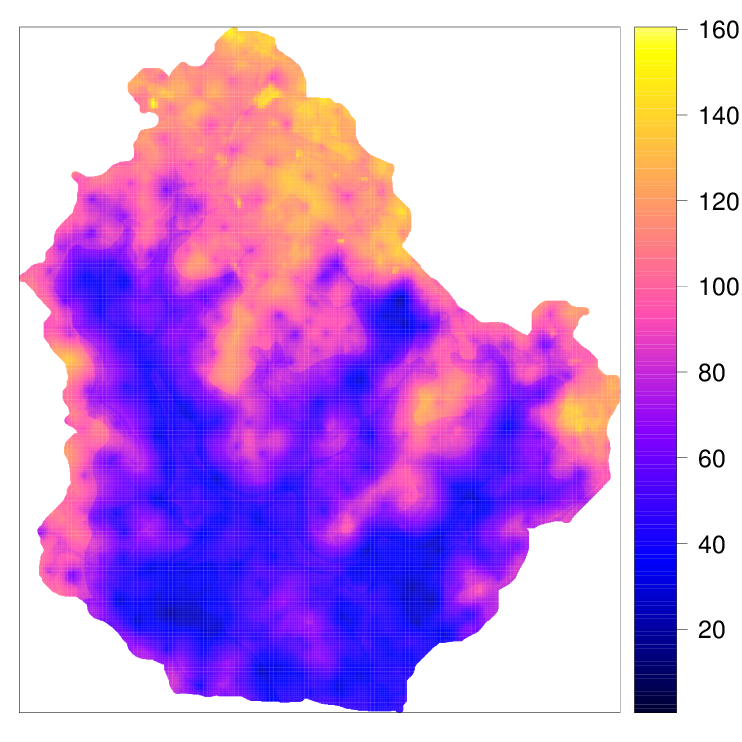
\includegraphics[width=60mm]{chap01FIG8a}
    \end{minipage}
    \begin{minipage}[b]{63mm}
      \subcaption{}
      \label{fig:clay-best-var}
      \centering
      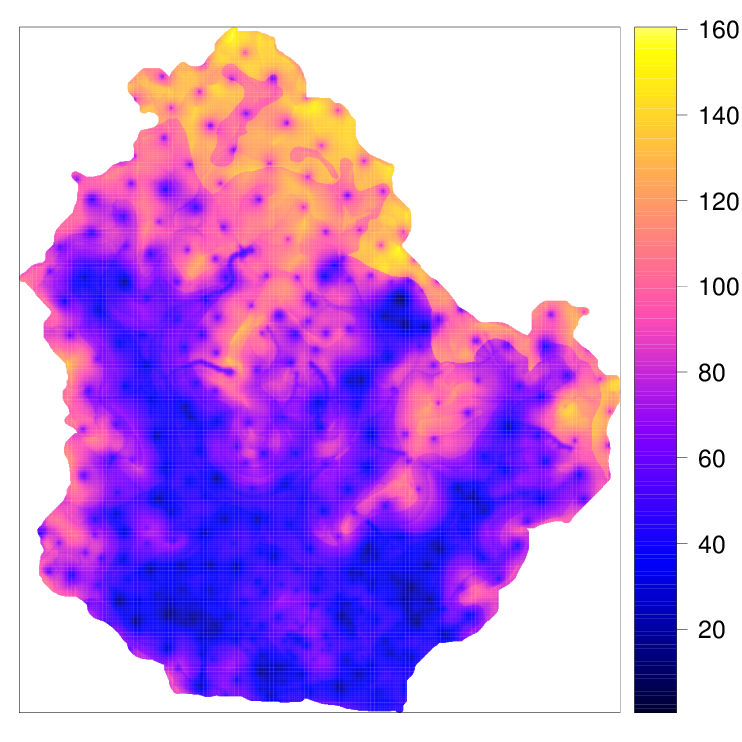
\includegraphics[width=60mm]{chap01FIG8d}
    \end{minipage}
    \begin{minipage}[b]{63mm}
      \subcaption{}
      \label{fig:soc-base-var}
      \centering
      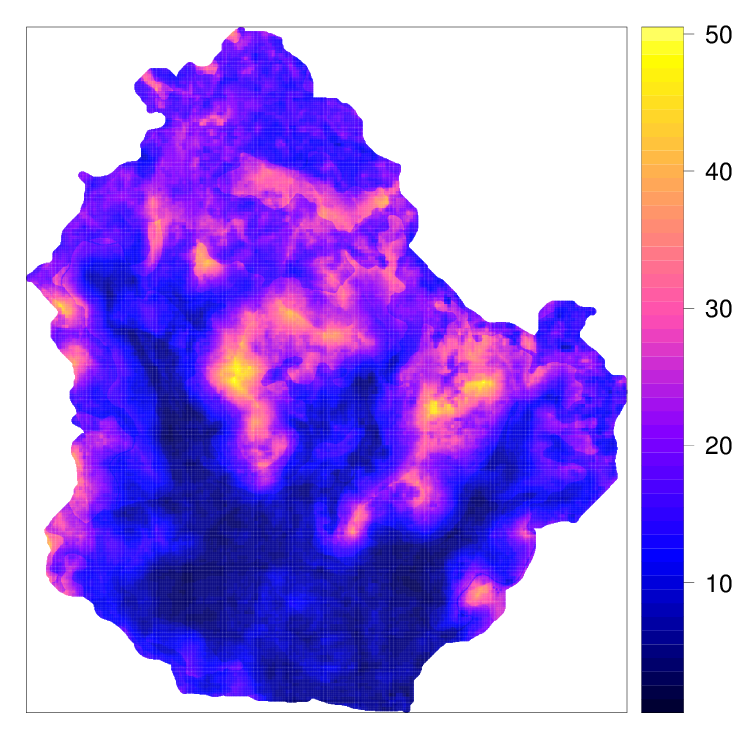
\includegraphics[width=60mm]{chap01FIG8b}
    \end{minipage}
    \begin{minipage}[b]{63mm}
      \subcaption{}
      \label{fig:soc-best-var}
      \centering
      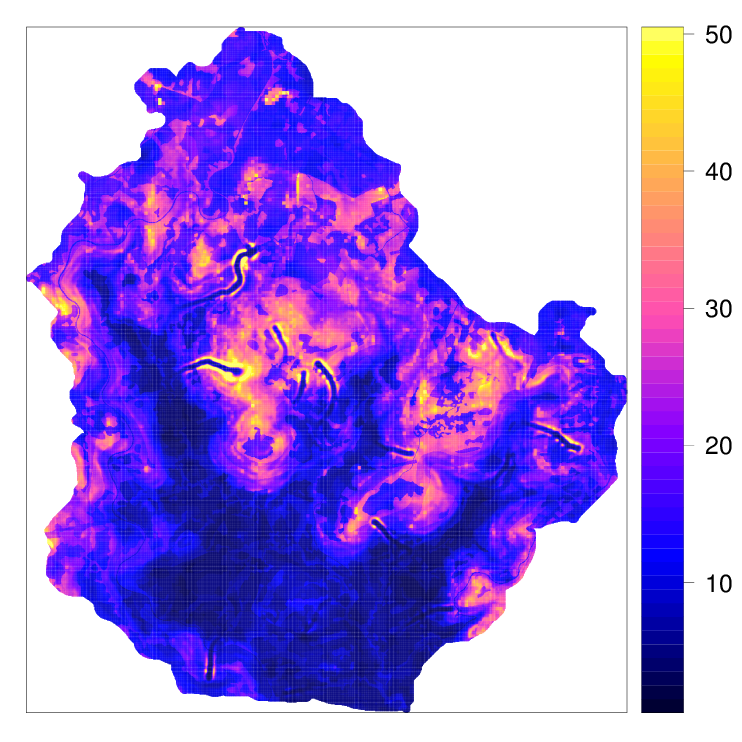
\includegraphics[width=60mm]{chap01FIG8e}
    \end{minipage}
    \begin{minipage}[b]{63mm}
      \subcaption{}
      \label{fig:ecec-base-var}
      \centering
      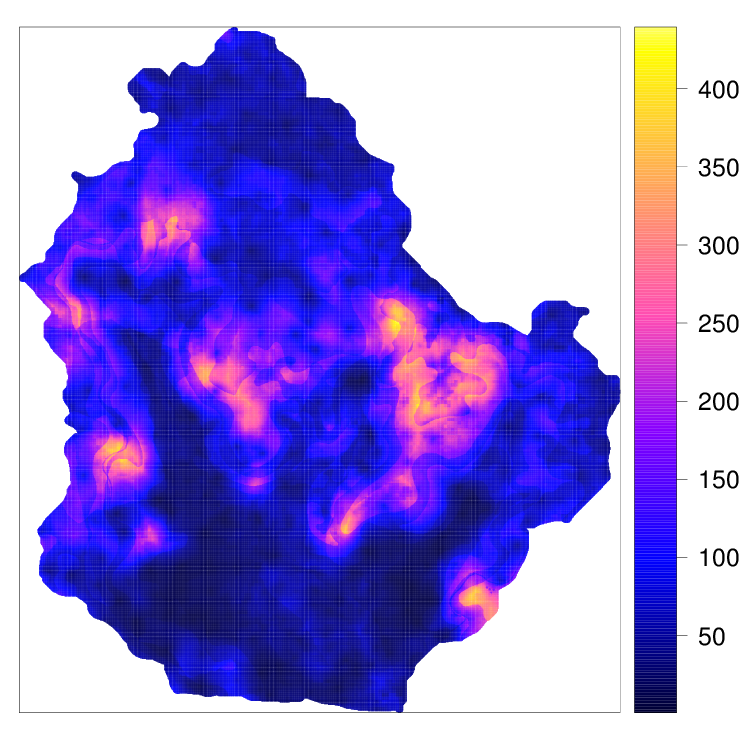
\includegraphics[width=60mm]{chap01FIG8c}
    \end{minipage}
    \begin{minipage}[b]{63mm}
      \subcaption{}
      \label{fig:ecec-best-var}
      \centering
      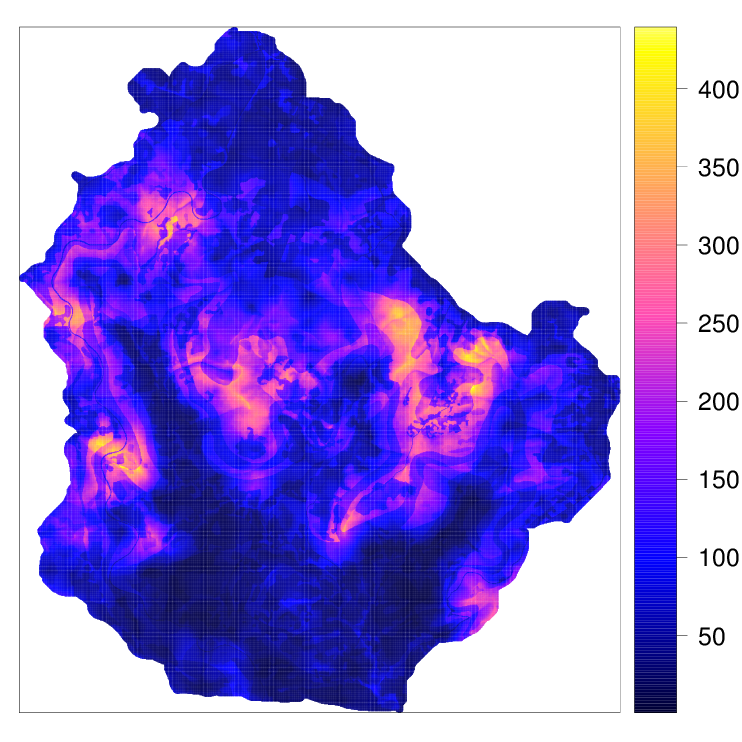
\includegraphics[width=60mm]{chap01FIG8f}
    \end{minipage}
  \caption{Prediction error standard deviations for CLAY (g~kg$^{-1}$) (a, b), 
  SOC (g~kg$^{-1}$) (c, d), and ECEC (mmol~kg$^{-1}$) (e, f) using the baseline 
  (left) and best performing (right) linear mixed models.}
  \label{fig:kriging-variance}
\end{figure}

The smallest prediction error standard deviations occur at lower elevations, 
along the three main streams, and close to the water outlet in the southern 
part of the study area. These areas have the highest density of point soil 
observations used to calibrate the models, and the smallest values for all 
three soil properties. While the first determines the accuracy of the EBLUP, 
the second influences the final accuracy through the back-transformation of 
predicted values.

\section{Discussion}

Our main goal was to evaluate whether investing in more spatially detailed 
environmental covariates improves the accuracy of soil maps. We saw that 
calibrating the models with more detailed covariates generally has a small to 
moderate, but positive, impact on the predictions. The magnitude of this 
benefit depends on the magnitude of the increase of the spatial detail of the 
covariate, on the other covariates included in the model, and on the soil 
property. However, there seems to be a limit above which the increase of spatial
detail has a negative impact on the predictions. In the next two subsections we
interpret the results from a pedological perspective and assess whether the 
investment in more detailed covariates is worthwhile or if alternatives to 
improve prediction accuracy should be favoured.

\subsection{Spatio-temporal controls of soil properties}

CLAY was moderately well predicted using less detailed environmental covariates,
with small improvement when using the more detailed covariates. CLAY was 
expected to have a strong correlation with topography and parent material. 
This correlation was already considerable when the less detailed DEM and 
geologic map were used, and improved only marginally with the more detailed 
version. One sensible explanation is that the effective (actual rather than 
theoretical) spatial detail of the two geologic maps was similar, although they
had a four-fold difference in the size of the minimum legible delineation (see 
\citet{HenglEtAl2006a} for a discussion on effective scale). For the DEM, many 
studies have already suggested that its resolution may be of secondary 
importance when calculating DEM derivatives for digital soil mapping 
\citep{ZhuEtAl2008, BehrensEtAl2010a, MillerEtAl2015}. The influence of land 
use on CLAY is currently small due to reduction of soil erosion in the first 
decade of the 21st century \citep{MiguelEtAl2012, TenCatenEtAl2012b}. A 
moderate within-field spatial variation may exist due to past erosional 
processes \citep{MouraBueno2012}, but we lack evidence of how well this source 
of variation was captured in the present-time point soil data.

It is worthwhile to consider the influence of the more detailed soil map on 
predicting CLAY. Due to its production process, the more detailed soil map 
derives a large amount of spatial detail from the geologic map, land use map 
and DEM -- note that the second-best performing model for CLAY included the 
more detailed geologic map instead of the more detailed soil map 
(\autoref{fig:model-series}). However, most of the additional spatial detail 
included in the more detailed soil map was probably based on the spatial 
variation of soil texture, because this is a strongly marked soil feature in 
the area \citep{MiguelEtAl2012}. Soil texture is one of the most important soil 
properties used by soil surveyors in the field to identify mapping units 
\citep{Legros2006}. These findings help explain why in the end the more 
detailed soil map was the most beneficial for CLAY instead of the geologic map.

SOC and ECEC were considerably better predicted when more detailed environmental
covariates were used. Our expectation that SOC and ECEC would have a strong 
correlation with land use was confirmed by the fact that this covariate 
explained a large amount of the variance and was highly beneficial for improving
the predictions. Although the available point soil data are limited to the 
2004-2011 period, we believe that land use changes in the last 30~years 
\citep{MiguelEtAl2012, TenCatenEtAl2012b} strongly affected SOC and ECEC. Thus, 
the more detailed land use map is likely to have considerably improved model 
performance because it is up-to-date and, possibly, because it has 40 times 
more spatial detail than its less detailed version. Despite the fact that the 
two land use maps used in this study were from different time periods, which 
confounds the analysis, the results obtained indicate that a more detailed land 
use map improves the prediction of SOC. For example, the areas used for crop 
agriculture, which are well know for having lower SOC and ECEC 
\citep{Menezes2008, MouraBueno2012}, are not depicted in the less detailed land 
use map.

We expected SOC to have a stronger correlation with the DEM than with the 
geologic map due to its strong dependence on erosion, but we observed the 
contrary. This result my be partially explained by the fact that there is a 
strong relation between geology and topography in the study area 
\citep{Sartori2009}. Due to its production process \citep{MacielFilho1990}, 
the geologic maps can be interpreted as an aggregated version of a DEM. A 
second sensible explanation is that the effect of erosion on SOC is not that 
large because erosion was considerably reduced in the last decade 
\citep{MiguelEtAl2012, TenCatenEtAl2012b}. A last possible explanation, which 
integrates the previous two, is the existence of a spatial relation between SOC
and CLAY, the last being strongly correlated with parent material. These 
relations help explain why the more detailed DEM was almost as beneficial as 
the more detailed geologic map for SOC predictions. In the case of ECEC, our 
expectation of a strong dependency on a more detailed geologic map for 
producing more accurate predictions was confirmed.

The observed benefit of the more detailed geologic map and DEM for making more 
accurate CLAY, SOC and ECEC predictions suggests that these soil properties are
spatially related in the study area. We also hypothesize that the complexity of
current land use makes it difficult to achieve SOC and ECEC models with 
performances comparable to CLAY. One important source of variation in 
forested areas is its use for animal grazing \citep{SamuelRosaEtAl2011a}. 
This influences nutrient cycling and soil nutrient availability 
\citep{SchramaEtAl2013}. Current remote sensing technology is unable to 
capture the data needed to proxy the environmental conditions created by
these processes.

\subsection{Using more detailed environmental covariates}

More detailed covariates are usually expected to improve predictions in digital 
soil mapping \citep{CavazziEtAl2013, MaynardEtAl2014}. However, deciding whether
to invest or not in more detailed covariates requires careful thinking and 
depends on case-specific elements. We generally saw improvement in the 
predictions in our study, but the improvement was not large and may not outweigh
the costs. Also, the models calibrated with the more detailed versions of all 
covariates were not the best performing models. Using more detailed satellite 
images and land use maps degraded CLAY predictions. Although the more detailed
soil map had the largest benefit for CLAY, it may be too costly and impractical 
since its production usually requires having available more detailed versions 
of all other covariates. For SOC and ECEC, simply using a more detailed land 
use map resulted in considerably more accurate predictions. However, the 
superior performance may not outweigh the extra costs because producing a more 
detailed land use map usually requires up-to-date field observations and 
satellite images. Thus, the decision to adopt a more detailed covariate for 
digital soil mapping will ultimately depend on a trade-off between the increased
accuracy and the extra budget required. It may also depend on other potential 
applications of the covariates, but this is not our concern here.

One interesting observation is that if a less detailed covariate yields poor 
predictions, its more detailed version has the potential to produce larger 
improvement in model performance. However, this is only a potential, not a 
guarantee. For instance, \citet{EldeiryEtAl2008} were not able to increase the 
$R^2 = 0.31$ of linear regression models of soil salinity by more than 0.07 
points using 7.5 times more detailed satellite images. On the other hand, model 
performance is likely to be hardly improved using more detailed covariates if 
their less detailed version has already produced accurate predictions. This 
agrees with findings by \citet{ThompsonEtAl2001} and \citet{KimEtAl2014}.

We also observed that the predictions can be degraded when using the more 
detailed version of covariates. In our study, this happened with the satellite 
image (all three soil properties), land use map (CLAY) and soil map (SOC and 
ECEC). A (small) benefit was observed only when these covariates were used 
along with the more detailed version of other covariates. As pointed out above,
such a small benefit may not outweigh the increase in mapping costs. The 
trade-off between reducing model performance and being beneficial seems to 
depend on how much more spatial detail a covariate will have and on its 
correlation with the soil property. For example, the land use map was strongly 
correlated with SOC and ECEC, but not with CLAY, and its more detailed version 
had 40~times more spatial detail. It helped improve SOC and ECEC predictions, 
but degraded CLAY predictions, resulting in only a small improvement when used
along with the more detailed satellite image and geologic map.

If the influence of a more detailed covariate depends on the increase of 
spatial detail, then the priority should be to improve the spatial detail of 
the most beneficial covariate. This requires solid subject area knowledge 
because empirical evidence from the baseline model may be insufficient. The 
most beneficial covariate is not necessarily that which explained the largest 
part of the variance in the baseline model (see \autoref{tab:drop}). This occurs
because increasing the spatial detail reduces the correlation between the 
covariate and the soil property. And also because there is little room to 
improve a correlation that is already high in the baseline model. 
\citet{CavazziEtAl2013} suggest that the more detailed covariate has an excess 
of detail, a ``noise'' that degrades the predictions. This could explain the 
results for \texttt{sat}: higher resolution images can resolve smaller objects
(e.g. individual plants) whose spectral behaviours are highly variable, adding
noise to the \texttt{sat}-soil property correlation; on the other hand, lower 
resolution images capture collections of objects, and thus their variation is 
smoothed out in the pixel, reducing noise.

According to information theory one should optimize (maximize) the correlation 
between the point soil data and the covariates. This was described elsewhere as 
matching the ``phenomenon scale'' (the spatial pattern of the soil property) 
with the ``analysis scale'' (the spatial pattern of the covariates) 
\citep{DunganEtAl2002, MillerEtAl2014}. Finding the ``optimum'' requires 
evaluating the strength of the correlation using covariates with different 
levels of spatial detail \citep{DragutEtAl2009, CavazziEtAl2013, MillerEtAl2015}.
Our results show that this approach may be too costly and impractical. Since 
digital soil mapping explores only the empirical relationship among 
environmental conditions and soil properties \citep{Grunwald2009}, the 
``optimum'' is a ``conditional optimum'' -- conditional on the point soil data 
available. It does not necessarily mean that the most accurate predictions will
be made, but only that there is a level of spatial detail at which the 
correlation between the covariate and the point soil data is at a maximum. We 
suggest that instead more comprehensive approaches should be used to explore 
the full potential of the available covariates (see \citet{BehrensEtAl2010a} and 
\citet{MillerEtAl2015} for examples).

Finally, one must still judge whether the potential improvement in predictions 
is sufficient given the extra costs involved with using more detailed covariates.
If the extra budget is spent on deriving more detailed covariates, we suggest 
that it may be better to substantially improve the detail of a less influential
covariate than marginally increase the detail of the most influential covariate.
However, other means to spend the extra budget should be considered. For 
instance, it may be more efficient to concentrate on obtaining more soil 
observations. These may focus on better capturing the short range spatial
variation \citep{BrusEtAl2007a} or improving the representation of the feature 
space to avoid undesirable extrapolations \citep{MinasnyEtAl2006b}.

\section{Conclusions}

This study has shown that:

\begin{enumerate}
 \item Using more detailed environmental covariates results in only a modest 
 increase in the prediction accuracy of linear prediction models;
 
 \item A more detailed covariate has a greater potential to improve prediction
 accuracy when the soil property is poorly predicted by its less detailed version;
 
 \item The impact on prediction accuracy when using the more detailed version 
 of a less important covariate may depend on which other covariates are included
 in the model;
 
 \item Choosing whether or not to invest in more detailed covariates depends on 
 the strength of the relationship between the covariates and the soil property 
 being modelled, and on the relative difference between the less detailed and 
 the more detailed versions of the covariates.
\end{enumerate}

\section*{Acknowledgements}

We are grateful to Dr.~Bradley A.~Miller, from the Leibniz Centre for 
Agricultural Landscape Research, M\"uncheberg, Germany, for his comments during 
the revision of the manuscript. The following colleagues collaborated in 
different phases of data collection and/or processing: Dr.~Ricardo Simão Diniz 
Dalmolin, Dr.~Edgardo Ramos Medeiros and Jean Michel Moura Bueno (UFSM), 
Dr.~Pablo Miguel (UFPel), Dr.~Mauro Antonio Homem Antunes, Fábio Paes Leme 
Ferreira, and Anastácia Perci Campos de Almeida (UFRRJ), and Luis Fernando 
Chimelo Ruiz (UFRGS). We are grateful to Dr.~Bas Kempen, Dr.~Tom Hengl, and 
Marcos Angelini (ISRIC) for their helpful comments during the conception of the
study and data analysis. We also thank the development teams and module/package 
authors of the many free and open source software (FOSS) and operational system 
(OS) that were used to develop our study. The first author was supported by the
CAPES Foundation, Ministry of Education of Brazil (Process BEX 11677/13-9). The 
last author was supported by the CNPq foundation, Ministry of Science and 
Technology of Brazil. The use of the RapidEye images is endorsed by the 
Corporate Commitment Agreement signed between the Federal Rural University of 
Rio de Janeiro and the Brazilian Ministry of the Environment.

\section*{Note}
This chapter is based on A.~Samuel-Rosa, G.B.M.~Heuvelink, G.M.~Vasques, 
L.H.C.~Anjos. Do more detailed environmental covariates deliver more accurate 
soil maps? \textit{Geoderma}, v.243--244, p.214--227, 2015.

% \section*{REFERENCES}
% \bibliography{biblio.bib}
 % 1. General introduction
% \artigotrue
\chapter{MODERN SOIL SPATIAL MODELLING AND ITS SOURCES OF UNCERTAINTY}
\shorttitle{Uncertainty in Soil Spatial Modelling}
\label{chap:chap02}

\def\enkeys{Demand for Soil Information. Mixed Model of Spatial Variation. Soil and Covariate Data. Model 
Structure.}
  
\begin{chapterabstract}{english}{\enkeys}
The efforts of the soil science community have motivated the scientific community to recognize the importance 
of soils for humanity and the environment at the local, regional, and global levels. Soil spatial modellers 
seem to have been able to convince policy and decision makers about the importance of producing and updating 
soil information. For that end, soil spatial modellers have been using the mixed model of spatial variation 
(MMSV). The MMSV integrates aspects of \q{traditional} methods of soil spatial modelling, based on the discrete 
model of spatial variation (DMSV), as well of geostatistical techniques, more formally the continuous model of 
spatial variation (CMSV). As such, the MMSV explores the knowledge of soil-forming factors as well as the fact 
that the soil is a continuous media. It also acknowledges that soil maps always deviate from the \q{truth}, 
which means that a soil map conveys what we expect the soil to be, not our certainty about it. There are many 
sources for our uncertainty about the soil. For instance, the soil and covariate data used to calibrate soil 
spatial models is an important source of uncertainty. Soil data can have errors and poorly represent the 
population from which it has been sampled. The influence of the covariate data on our uncertainty about the 
soil expresses itself through the poor correlation with soil properties. Finally, the structure of the model 
used to measure the empirical correlation between covariates and soil properties can greatly determined our 
uncertainty about the soil. Because we cannot eliminate the uncertainty of a soil map, our knowledge about the 
soil will always be limited. Despite of this, soil spatial models are still needed to guide our every-day 
actions.
\end{chapterabstract}

\formatchapter

\section{DEMAND FOR SOIL SPATIAL INFORMATION}

\def\footmodeller{\footnote{The use that I give to the expression \emph{soil spatial modeller} throughout this 
thesis is approximately equivalent to expressions traditionally used in the academic world such as soil 
scientist, soil surveyor, soil taxonomist, geostatistician, pedometrician, soil investigator, soil mapper, and 
so on. In this thesis, a soil spatial modeller is any person that \emph{constructs} an explanation -- a model 
-- of the observed spatial soil variation using the tools and techniques available at his/her time and place. 
The goal of a soil spatial modeller is to construct a model that is simple yet able to produce an accurate 
representation of the spatial soil variation given the available resources and its intended application. I call 
this activity \emph{soil spatial modelling}. Accordingly, I understand that those that are excluded from the 
academic world such as peasants, farmers, indigenous populations, and so on, are soil spatial modellers as 
well, although their modelling of the soil is not the focus of this thesis.}}

Many soil spatial modellers\footmodeller{} have complained for many years about the decreasing interest in 
producing and updating soil information, not only in Brazil \cite{Dalmolin1999, Ker1999, KerEtAl2003, 
Mendonca-SantosEtAl2003, Ramos2003, Espindola2008}, but in many countries around the world \cite{Basher1997, 
HarteminkEtAl2008, Grunwald2009, SanchezEtAl2009, Finke2012, SamuelRosa2012}. Several reasons were presented to 
explain the general lack of interest in producing and updating soil information after the 1980s: the use of 
specialized taxonomic terminology by soil spatial modellers was abusive; information conveyed by soil maps was 
too limited due to its qualitative nature; policy and decision makers were unaware of the usefulness of soil 
information and dynamicity of soil; applied scientific research came to be preferred over basic scientific 
research; soil spatial modelling largely ignored environmental applications other than agriculture; lack of 
communication between soil spatial modellers and the general public; among others. But everyone seem to agree 
on one point: governments understood that producing and updating soil information was too costly. Cutting down 
the budget for soil spatial modelling fundamentally was an economic decision.

Since the last decade, soil scientists in general have launched many initiatives to make soil become a hot 
topic \cite{HarteminkEtAl2008}. For example, the United Nations (\WorldSoilDay) declared 5 December the World 
Soil Day and 2015 the International Year of Soils \cited{in an effort to raise awareness and promote more 
sustainable use of this critical resource}. Soil spatial modellers created a global consortium, the \gsm, with 
the goal of producing \cited{a new digital soil map of the world using state-of-the-art and emerging 
technologies}. The Food and Agriculture Organization (\fao) launched a Global Soil Partnership (\gsp) for 
\cited{leading to the adoption of sustainable development goals for soils}. The International Union of Soil 
Sciences (\iussusc) created a working group, funded by the United States Department of Agriculture (\usdausc) 
to develop a Universal Soil Classification System, \cited{a common language to describe soils that can be used 
internationally}. An Intergovernmental Technical Panel on Soils (\itps) was formed with soil experts from all 
regions of the world \cited{to provide
scientific and technical advice and guidance on global soil issues to the Global Soil Partnership}. The 
\gates{} foundation handed out an \SI{18}[\$]~million grant \cited{to map most parts in Sub-Saharan Africa, and 
make all Sub-Saharan Africa soil data available}. Soil spatial modellers at the International Soil Reference 
and Information Centre (ISRIC) launched its Global Soil Information Facilities (\gsif), a \cited{framework for 
production of open soil data}, which has already output \SI{250}{\m}-resolution soil maps with global coverage. 
In Brazil, soil spatial modellers created the Brazilian Network for Research in Digital Soil Mapping (\redemds) 
with the objective of \cited{generating synergy among Brazilian soil scientists to advance research in digital 
soil mapping}.

\def\footpronassolos{\footnote{The initiative to restart the national soil survey program coincides with the 
currently increased, government funded, economically driven, historical pressure to occupy the Cerrado and 
Amazon biomes, considered \q{the last agricultural frontier} \cite{Correia2005, Macarini2005, Silva2005, 
CarvalhoEtAl2009, Batlle-BayerEtAl2010, MartinelliEtAl2010, SchneiderEtAl2015}. It is traditionally argumented 
that transforming parts of the Cerrado and Amazon biomes into agricultural land is needed to eradicate poverty 
in Brazil and feed a growing world population. This is the argument used by the Brazilian politicians who are 
in favour of changing the Brazilian legislation to easy the acquisition of up to \SI{100000}{\hectare} of 
agricultural land in these regions by multinational corporations to produce cellulose and paper 
\cite{SECOM2015}. Unfortunately, the Brazilian states that compose \q{the last agricultural frontier}, which 
are among the poorest Brazilian states, have a long history of land conflicts due to the conservative 
development model adopted in Brazil, where the benefits of economic growth are not shared by all people 
\cite{ComissaoPastoraldaTerra2015}. In regions such as this, the problem of food insecurity is more due to the 
lack of political will than to the lack of food \cite{FAO2005, FAO2009, FAO2015}. As such, one might wonder 
whether restarting the national soil survey program without promoting a deep agrarian reform and strengthening 
of the public agricultural extension service is beneficial for the general Brazilian population.}}

The efforts of the soil science community have motivated the scientific community to recognize the importance 
of soils for humanity and the environment at the local, regional, and global levels \cite{SanchezEtAl2009, 
Kempen2011, OmutoEtAl2013}. Soil scientists, whose presence in public administration through scientific and 
technical advisory boards appears to grow, seem to have been able to convince policy and decision makers about 
the importance of producing and updating soil information. For example, in Brazil, the Federal Court of 
Accounts (\tcu), in collaboration with Embrapa Soils and other soil science related institutions, held a Soil 
Governance Conference, where a new National Program for Soil Survey and Interpretation of Brazil (\pronassolos) 
was announced, with an expected budget of \SI{8}[R\$]~billion\footpronassolos. In the sequence, Embrapa Soils 
created a working group, with soil spatial modellers from other government institutions and universities, and 
the first PRONASOLOS report with proposal and goals was completed on December 2015. Unfortunately, it is not 
clear whether the national soil survey program will truly be restarted because, like happened in the end of the 
1980s, it essentially is an economic decision. Apparently, other areas of soil science have not been receiving 
much more attention and/or funding than soil spatial modelling. It is also not clear whether the soil science 
community efforts have brought about a renewed recognition of the importance of soils for humanity and the 
environment among the general public.

\section{MODERN SOIL SPATIAL MODELLING}

Technology plays a determinant role on how we perceive the world around us -- see, for example, 
\citeonline{Hartemink2009}. When early farmers, during the Neolithic Revolution, ca.~\num{10000}~years ago, 
first observed that soil properties varied in space, they probably soon figured out that such variation was 
related to other environmental features and influenced crop yields. That early, rough, approximate 
understanding -- a \emph{model} -- of soil spatial variation certainly was fundamental for choosing -- 
\emph{predicting} -- the most appropriate locations to start and maintain human settlements, some of which 
became great, long-standing empires \cite{MazoyerEtAl2008, BrevikEtAl2010, Churchman2010}. Archaeological 
research provides evidence that several of these empires had more formal \emph{soil classification systems} and 
\emph{soil survey programs}, in most cases for taxation purposes \cite{Barrera-BassolsEtAl2003} -- a practice 
that lasts till today.

\def\footKubrick{\href{https://www.youtube.com/watch?v=qtbOmpTnyOc}{\textit{2001: A Space Odyssey}}}

A lot happened since the Neolithic Revolution \cite{BrevikEtAl2010} -- from bone to spacecraft, as in Kubrick's 
-- \footKubrick,
and the knowledge constructed with multiple soil spatial studies was fundamental for the development of 
agriculture and increase of food production -- although many farmers still live in Neolithic conditions 
\cite{MazoyerEtAl2008}. If we adopt an integrative view, soil maps produced during this long period of human 
history seem to fit into what we call today the \emph{discrete model of
spatial variation}. The discrete model of spatial variation explains the variation of soil properties in space 
using mutually exclusive mapping units that are separated by sharply defined, crisp boundaries (i.e. polygons) 
\cite{Heuvelink1996, Legros2006}. The soil in each mapping unit is more or less homogeneous with regard to its 
properties at the time of mapping. These properties, which are generally used to name the mapping unit along 
with other environmental features, can be characterised using one or more direct observations made within the 
domain of the mapping unit \cite{WebsterEtAl1990, Legros2006}.

\subsection{Discrete Model of Spatial Variation}

A key step was given in 1886 in Russia with the formalization of the approximate understanding of the soil 
spatial variation using scientific parlance, i.e. the postulation of the \q{the basic law of soil science} by 
Vasily Dokuchaev \cite{Florinsky2012}: \q{Any... soil is always and everywhere a mere function of the following 
factors of soil formation: 1) the nature (content and structure) of the parent rock, 2) the climate of the 
given terrain, 3) the mass and character of vegetation, 4) the age of the terrain, and finally, 5) the terrain 
topography.}. The basic law of soil science was presented 40-years later by Sergey Zakharov in the form of a 
general soil formation equation, which is known in the western soil science literature as \cite{Jenny1941, 
Florinsky2012}

\begin{equation}\label{eqn:chap02-clorpt}
 soil = f(cl, o, r, p, t, \ldots),
\end{equation}

\noindent where $soil$ is the soil and its properties, $cl$ if the climate, $o$ 
are the organisms, including humans, $r$ stands for relief or topography, $p$ is the 
parent material, $t$ is time or age of the terrain, and $\ldots$ stand for other unknown 
players. Dokuchaev was aware that producing empirical evidence to corroborate his basic law of soil science was 
difficult because data on soil formation factors was scarce. Besides, it was difficult to numerically express 
the relation between soil and formation factors. Despite of these difficulties, the basic law of soil science 
was readily adopted by soil spatial modellers because it provided a solid basis for explaining the soil spatial 
variation \cite{Smith1986}.

An important enthusiast and supporter of the use of \autoref{eqn:chap02-clorpt} was Hans Jenny 
(\citeyear{Jenny1941}). He believed that the large volume of already existing soil data/knowledge, which had 
been constructed mostly based on the basic law of soil science, needed to be organized by means of numerical 
laws and quantitative theories -- instead of soil maps, taxonomic classifications, and soil-forming processes 
-- to enable treating it mathematically (i.e. using empirical correlation). For that end, solving 
\autoref{eqn:chap02-clorpt} depended on the soil scientist' skills to select suitable study areas and locations 
for making observations. But the problem continued to be that obtaining data on soil-forming factors was still 
difficult compared to obtaining soil data. It follows that direct application of \autoref{eqn:chap02-clorpt} 
for producing soil maps was impossible because it required soil-forming factors to be exhaustively known 
everywhere \cite{Jenny1941}. Despite the operational difficulties encountered since the postulation of the 
basic law of soil science and definition of \autoref{eqn:chap02-clorpt}, the concept of soil-forming factors 
were employed in most of the subsequent soil spatial studies around the world, resulting in the enhancement of 
taxonomic classifications, theories about soil-forming processes, and production of soil maps using the 
discrete model of spatial variation \cite{Schelling1970, Hudson1992, BockheimEtAl2000, Legros2006, 
KrasilnikovEtAl2009b, HarteminkEtAl2013}.

Soil spatial modelling using the discrete model of spatial variation and the idea that soil properties were 
determined by soil-forming factors had its weaknesses as any other model of spatial variation. Three main 
weaknesses can be pointed out, all of which only were recognized and understood using post-war 
scientific/technological developments \cite{HeuvelinkEtAl2001, McBratneyEtAl2003, ScullEtAl2003}. First, 
\q{soil bodies} were described as discrete, homogeneous entities -- although it was recognized that soil is a 
continuous media whose properties vary from place to place in such a way that nearby locations have more 
similar soil property values than distant locations (spatial autocorrelation) --, implying that the fluxes of 
energy and matter across the landscape had to be understood as being partially homogeneous (within a mapping 
unit), partially discontinuous (between mapping units) processes. Second, the uncertainty (errors) about mapped 
soil properties was disregarded, meaning that a single, absolute value for each soil property would be 
attributed to each mapping unit ignoring that soil properties vary from place to place and that estimates can 
be affected by all sorts of errors. Last, but not least, some important soil spatial modelling decisions could 
not be efficiently shared with others by means of formal, explicit knowledge because they were largely based on 
the intuitive, tacit knowledge of soil modellers, i.e. the knowledge that a soil modeller has about the 
soil-landscape relationships and the soil modelling process but that cannot be adequately communicated, 
articulated by verbal (written or spoken) means. This was evidenced, for example, by the fact that different 
soil modellers would produce considerably different soil maps without being able to explain why 
\cite{Legros2006, BazagliaFilhoEtAl2013}.

\subsection{Continuous Model of Spatial Variation}

Different solutions were explored during the post-war to overcome one or another weaknesses of the discrete 
model of spatial variation. Most of these solutions came from the new developments in the fields of 
mathematics, statistics and informatics, many of them already successfully employed by the mining industry 
\cite{Matheron1969}. For example, those important soil spatial modelling decisions, generally taken with basis 
on the tacit knowledge of the soil modeller, could now be more efficiently communicated with others through the 
use of computers -- provided they had a computer. This is because using a computer to produce soil maps 
requires modelling rules to be formalized in the form of a computer script, which is the mean used to establish 
the communication between the soil modeller (a human being) and the data processing environment (a computer).

Soil modellers also understood that the error about the mapped soil property could be acknowledged using 
classical statistics. First, the definition of mapping units, which was based on the knowledge of the 
soil-forming factors, needed to be viewed as a modelling exercise that aims at minimizing the within-unit 
variance (and maximizing the between-unit variance) of a soil property \cite{VoltzEtAl1990}. Then, the most 
likely value of a soil property at any one point in a given mapping unit would be its mean over the multiple 
observations made in that mapping unit \cite{VoltzEtAl1990, Cressie1993}. The only requirement -- so that the 
estimated mean would be fair (unbiased) -- was that the location of soil observations be selected using some 
form of randomization (probability sampling) such as it is done in controlled agronomic experiments, e.g. 
simple random sampling within mapping units \cite{deGruijterEtAl1990}. It follows that the uncertainty about 
the value of the mapped soil property is the same everywhere within a mapping unit, irrespective of the 
location of existing soil observations \cite{Heuvelink1996}. This is because due to statistical independence 
and constant variance within mapping units, the expected error of predicting the value of a soil property at 
any location with its mean is also the same everywhere.

Those solutions still required describing \q{soil bodies} as discrete, homogeneous entities, and continued 
neglecting the spatial variation and autocorrelation of soil properties. For that end, one solution was to 
ignore the knowledge on soil-forming factors and use the \emph{continuous model of spatial variation}. 
Accordingly, the main requirement was that a soil property be treated as the outcome of a random (stochastic) 
spatial process \cite{Cressie1993, Webster2000}. At first, the proposition of \emph{imagining} the soil as 
being the result of randomness is awkward (\autoref{eqn:chap02-clorpt}). However, pondering on the multitude of 
soil-forming factors and processes, and on the complexity of their interactions \cite{BockheimEtAl2010, 
GrunwaldEtAl2011}, as well as on the limitations of the existing knowledge on soil spatial variation, one can 
easily conclude that soil is a chaotic media \cite{Webster2000} -- so why not treat it as such? One only had to 
\emph{imagine} that the value of a soil property observed at a given location simply was one that happened to 
be recorded by chance among an infinitely large number of values that could have been recorded instead 
\cite{Webster2000}. In other words, one had to \emph{imagine} that, if a soil property is recorded multiple 
times at the same location, the recorded values would not necessarily be the same. As such, a soil property at 
a given location would not be described using a single absolute value, but a probability distribution function 
(PDF), generally the normal (Gaussian), characterised by the mean and variance of those \q{recorded} values. 
Accordingly, to describe the fact that soil property values at nearby locations are more similar than at 
locations further apart -- they covary, vary together or jointly -- would require a joint probability 
distribution function, characterised by the covariance \cite{WebsterEtAl1990, Cressie1993}.

Different from its discrete counterpart, the continuous model of spatial variation takes into account the 
relative location of existing observations when predicting a soil property at a given unobserved location. In 
the simplest case, the most likely value of a soil property in a given location is defined by a constant mean 
computed over all observations made in the mapping region, plus a random variable with mean zero and (spatial) 
covariance that depends only on the separation distance between locations \cite{WebsterEtAl1990, Cressie1993}. 
The main idea underlying the continuous model of spatial variation is that soil property values at nearby 
locations are more similar than at locations further apart \cite{WebsterEtAl1990}. Thus, we err less if we 
predict the value of a soil property at a given location with a value observed at a nearby location than with a 
value observed at a distant location. Optimally, because the soil is a continuous media and its properties vary 
in space in an autocorrelated fashion, we make the most accurate prediction taking a weighted average of the 
values recorded at all observation locations, nearby locations receiving larger weights than distant locations. 
In both cases, it follows that the uncertainty about the mapped soil property is larger the farther from 
existing soil observations, i.e. it is spatially varying \cite{Cressie1993}.

% The obvious difficulty in this approach is that the PDF cannot be defined because we usually 
% have one single value recorded at each observation location.

\subsection{Mixed Model of Spatial Variation}

Availability of general-purpose computers fuelled the use and development of the continuous model of
spatial variation, especially in European, North American, and Oceanian countries
\cite{HeuvelinkEtAl2001, McBratneyEtAl2003, ScullEtAl2003}. But limitations in its prediction
performance and developments in remote sensing and machine-learning algorithms helped many soil
scientists to understand that the continuous model of spatial variation had limitations too. For
instance, it is unable to capture abrupt changes in the values of soil properties that occur, for
example, between agricultural fields, parent materials, land uses, and so on
\cite{SteinEtAl1988, VoltzEtAl1990}. Because, contrary to the discrete model of spatial variation, the
continuous model of spatial variation largely ignores the existing pedological knowledge
\cite{Grunwald2009, Lark2012}. Soil scientists also understood that the discrete model of spatial
variation was more efficient than previously thought \cite{BregtEtAl1987}. First, because it was now
possible to employ Jenny's equation of soil-forming factors for soil mapping using remote sensing
products as surrogates of the factors of soil formation \cite{MooreEtAl1993}. Second, machine-learning
algorithms enabled identifying complex spatial patterns that before could only be identified by an
experienced soil scientist \cite{McKenzieEtAl1999}. The most logical step was to combine the
strengths of both discrete and continuous models of spatial variation into a single model -- the
\emph{mixed model of spatial variation} --, that is, inclusion of the existing pedological
knowledge and consideration of the spatial continuity of soil property values.

The mixed model of spatial variation\footnote{The use that I give to the expression \emph{mixed model of 
spatial variation}
in this thesis is approximately equivalent to expressions such as regression-kriging, kriging with external 
drift, universal
kriging, hybrid approach for soil mapping, pedometric mapping, digital soil mapping, predictive soil mapping, 
environmental
correlation, geostatistical mapping, soil-landscape modelling, and so on. As far as I know, soil modellers have 
not yet reached an agreement on how these \q{traditional} expressions should be used, nor what their 
\q{correct} meaning is. See, for example, \citeonline{Hengl2003, McBratneyEtAl2003, ScullEtAl2003}. Because the 
expression \emph{mixed model of spatial variation} has a theoretical basis (other expressions are defined based 
on operational aspects), I understand that its adoption and use is a more appropriate choice.} can be viewed as 
a generalization of previously existing models of spatial variation, by which a soil property 
$Y(\boldsymbol{s})$ at a given location $\boldsymbol{s}$ is modelled as the outcome of a spatial stochastic 
process \cite{Cressie1993, HeuvelinkEtAl2001, LarkEtAl2006}. Accordingly, the model is composed of \emph{fixed} 
and \emph{random effects}. The fixed effects, a deterministic large-scale spatial trend, $m(\boldsymbol{s})$, 
describes the portion of the spatial variation of the soil property that is explained with the factors of soil 
formation as suggested by the empirical correlation calculated using point soil observations and spatially 
exhaustive covariates\footnote{In the statistical literature, the term \emph{covariate} is synonymous to 
\emph{explanatory variable}, \emph{predictor variable}, and \emph{independent variable}, and refers to the 
variable that, although not being of primary interest, is used in a model because it determines the behaviour 
of the \emph{response variable} or \emph{dependent variable} \cite{Everitt2006}. In soil science, a covariate 
has the same statistical meaning, the difference being that they assume a pedological meaning as well, i.e. 
they are viewed as proxies, indicators, substitutes, surrogates, approximations of the soil-forming factors due 
to the simple fact that the soil-forming factors -- the true environmental conditions that helped shape the 
soil -- are unknown. Covariates are defined \emph{spatially exhaustive} when they cover the entire area being 
modelled, i.e. they are exhaustively known in the entire geographic space.}. The random effects, also known as 
stochastic residuals or latent variables, $e(\boldsymbol{s})$, describe the portion of the spatial variation of 
the soil property that cannot be explained with the covariates but is potentially spatially correlated, the 
form and degree of this spatial correlation possibly being interpreted pedologically \cite{Lark2012}. Thus

\begin{equation}\label{eqn:intro-mixed-model}
Y(\boldsymbol{s}) = m(\boldsymbol{s}) + e(\boldsymbol{s}).
\end{equation}

\autoref{eqn:intro-mixed-model} possesses a great flexibility that facilitates to explore newly developed 
statistical and data-mining methods, generally resulting in better performance than the constituent models 
alone, as well as integrating the existing pedological knowledge provided it is translated into a mathematical 
form \cite{OdehEtAl1994, OdehEtAl1995, Heuvelink1996, McBratneyEtAl2000, HenglEtAl2004, Lopez-GranadosEtAl2005, 
WebsterEtAl2007, Grunwald2009, Lark2012}. These features promoted the rapid popularization of the mixed model 
of spatial variation, and many recent large scale soil-mapping projects already successfully employed the mixed 
model of spatial variation \cite{PoggioEtAl2014, NussbaumEtAl2014, HenglEtAl2015}.
% and the development of the Internet, 

% Unfortunately, along with the success of the mixed model of spatial variation, came a rupture between soil 
% modellers pertaining to different \q{schools}, building a negative atmosphere in many
% countries (see examples from Brazil [\url{https://groups.google.com/forum/#!forum/soil-mapping}] and
% Spain [\url{http://www.madrimasd.org/blogs/universo/2009/10/07/126094}]). On one side, this was
% caused by the (presumptuous) assumption that the mixed model of spatial variation possibly
% represented a \q{paradigm shift} in soil science \cite{McBratneyEtAl2003} and that it is the
% ultimate soil mapping method, superior to all others \cite{MinasnyEtAl2016}. This assumption is
% certainly untrue, specially in many poorer regions where the mixed model of spatial variation seems
% useless because farmers already obtain satisfactory yields and properly manage their soils using
% indigenous/local knowledge
% \cite{Barrera-BassolsEtAl2003, Barrera-BassolsEtAl2006, HillyerEtAl2006, CorreiaEtAl2007, 
% ValeJuniorEtAl2007}.
% Perhaps the strong criticism made against soil scientists that
% refused to adopt the mixed model of spatial variation, using somewhat pejorative arguments
% \cite{HeuvelinkEtAl2001,Mendonca-SantosEtAl2003}, helped building this unfruitful scenario. On
% the other side, soil scientists disliked losing importance in the research field in which they worked for
% decades, perhaps very afraid of the new technological developments due to their poor knowledge of
% mathematics, statistics, and informatics \cite{Webster2001,SamuelRosa2012}.

% Although all that is very common when a new theory or method appears
% \cite{Russell1932, Feyerabend1977, Kuhn2011}, I think we have reached a point in which nothing else
% can be gained by
% playing one soil scientist against the other. Such a (noble) understanding was already shared by
% \citeonline{Jenny1941} when comparing \cited{soil geographers} and \cited{soil functionalists}.

\subsection{Spatial Soil Modelling Steps}

Despite the rapid technological developments observed recently, the activity of modelling the soil remained 
essentially the same throughout human history. Soil maps still serve the same old purpose of representing our 
limited understanding about the spatial
organization of the soil in the natural environment in a simplified manner, as well as giving insights about 
how the soil came to be and how they should be managed \cite{Jenny1941, Hudson1992, Legros2006, 
Blanco-CanquiEtAl2010, Grunwald2010}. For this reason, irrespective of the method/model used to produce soil 
maps, perhaps we should use an (integrative) expression such as \emph{soil spatial modelling} instead of 
picking one of the many currently used.

It follows that, based on the existing body of knowledge on soil spatial modelling and the currently available 
technologies, we should try to define what it constitutes, in practice, the soil spatial modelling activity. A 
suggested general (didactic) sequence of steps that we believe represent what is or should be done in soil 
spatial modelling is presented below.

\begin{description}
\item[Step 1] Identify a reality or problem entity, the geographic region for which
there is a demand of spatial soil information. Target soil properties are appointed as well as the
required accompanying output information (e.g. metadata). Key modelling decisions are taken in this step
such as the support (punctual or areal), spatial resolution (and possibly the cartographic scale),
coordinate reference system, etc. Depending on how well defined the demand is, the model of spatial
variation can also be specified, i.e. discrete, continuous, or mixed. Data policy is discussed (What data
should be public? How to make data public? How to implement the data policy?) and agreed upon. Finally,
the available infrastructure, budget, time, and workforce are specified so that next steps can be
appropriately planned as to fulfil the demand.

\item[Step 2] Develop a conceptual model of pedogenesis, a verbal representation of the
reality or problem entity including the explicit description of soil-forming factors and processes
that determine the spatio-temporal distribution of soil properties. This requires gathering the most
of the existing environmental information contained in scientific articles, technical reports,
books, websites, local knowledge, as well as existing maps of the soil, land use, geology, digital
elevation models, satellite images, aerial photographs, among others. Environmental information is used
to articulate pedogenetic concepts. Provided that any of the existing soil data are available, an
exploratory data analysis can help unravelling soil-landscape relationships. The poorer the volume of
existing environmental information, and the less experienced the soil modeller is, the more
important an exploratory field campaign is to help understanding the existing soil-landscape relationships.

\item[Step 3] Define the model of spatial variation, a translation of the conceptual
model of pedogenesis into a set of possible mathematical representations. Depending on
how well defined the demand was, the model of spatial variation was already specified in
\textbf{Step 1}. Provided the volume of existing environmental information and legacy soil data is
moderate to large and/or the soil modeller is very experienced and/or the available budget
allows carrying out exploratory field campaigns, a single model of spatial variation is
defined, i.e. discrete, continuous, or mixed. Assuming that the mixed model of spatial variation is
chosen, the statistical and/or data-mining models that will be used to represent the discrete
and continuous components are specified, taking into account the feasibility of meeting their
requirements given the available soil data, infrastructure, budget, time, and workforce. If multiple
models or statistical and/or data-mining models are chosen, the pedological and
statistical criteria for identifying the best performing model are defined.

\item[Step 4] Prepare the modelling database, a collection of soil and covariate data
needed to estimate the parameters and test the chosen statistical and/or data-mining
models. If required, this includes preparing a sampling plan with formally defined selection rules,
making properly documented field soil observations, and running replicated laboratory analyses.
Soil data from different sources are harmonized. Covariates are selected using the conceptual model
of pedogenesis and empirical evidence. Both soil and covariate data are assessed regarding the need
for nonlinear transformations to meet the requirements of the chosen statistical and/or
data-mining models, and to improve their empirical correlation. Several of these tasks can be (and
usually are) carried out with the aid of a data processing environment (a computer).

\item[Step 5] Estimate the parameters of the statistical and/or data-mining
models, a task that essentially depends on translating the set of possible mathematical
representations of the conceptual model of pedogenesis into a computer representation, that is, a
computer code or script. Developing a well documented computer code that describes all processing
steps ease re-design, future consistency checks, correction of mistakes, and
dissemination/reproducibility. Calibrated models are evaluated using statistical criteria defined in
\textbf{Step 3} such as goodness-of-fit measures. Best performing models are evaluated regarding their
tenability (pedological evaluation), which includes visually assessing draft soil maps, and how well
they represent the range of possible mathematical models. Failure in this last assessment suggests
that the model requires adjustments, possibly more calibration data, or that it can be discarded.

\item[Step 6] Validate the statistical and/or data-mining models, preferentially
predicting the values of the modelled soil properties at a set of independent, probabilistically
selected observation locations for which the true values are known. If an independent set of
observation locations is unavailable, validation is performed using leave-one-out cross-validation.
The best performing model, selected using the statistical criteria defined in \textbf{Step 3}, is
assumed to be the best mathematical representation of the reality under study. If two or more
models present similar prediction performance and have a considerably different structure, then it
can be assumed that the best mathematical representation of the reality under study is given by the
aggregated version of these models, or parsimony is considered to elect the simpler model with 
fewer variables, steps, rules, etc. If previous steps have already allowed selecting a single best
performing model, statistical validation is used only to assess model accuracy.

\item[Step 7] Make spatial predictions, the application of the best performing
model(s) to predict soil properties values at unvisited locations. If demanded, the uncertainty
about the predicted soil properties values (i.e. the prediction interval) is estimated too.
Maps of the target soil properties as well as the required accompanying output information
(e.g. point soil observations, covariate maps, uncertainty maps, metadata, computer scripts)
are delivered to the users of the soil information, and possibly used to populate a spatial soil
information system, where they are made available for inspection using different visualization
techniques. Provided there is infrastructure, budget, time, and workforce available, modelling
steps can be re-designed and the outputs updated at the user request.

\item[Step 8] Reformulate the conceptual model of pedogenesis, the use
of the knowledge gained during the previous steps until the production of the soil property
maps, which give insights about the reality or problem entity under study, to correct
and/or improve the description of soil-forming factors and processes that determine the
spatio-temporal distribution of soil properties. If demanded, the reformulated conceptual model
of pedogenesis is delivered to the users of the soil information as well to help in scenario analysis
and decision making.
\end{description}

\section{SOURCES OF UNCERTAINTY IN SOIL SPATIAL MODELLING}

Soil spatial models, like any other model, are nothing more than a gross simplification of reality.
This means that soil models are unable to explain the spatio-temporal soil variation in
its entirety, but only a small part of it \cite{Heuvelink1998a, Legros2006}. When we use a
soil-mapping model to produce continuous representations of soil properties across space and/or time,
i.e. soil maps, these continuous representations will inexorably deviate from the \q{truth}. What
the soil map presents is our most likely expectation about the soil properties -- not our
\emph{certainty} about them. The deviation from the \q{truth} is what we call \emph{error}. Many
examples from the soil-mapping literature show that, irrespective of the soil property, soil-mapping
models have a quite variable predictive performance, usually explaining between \SI{15}{\percent}
(or less) and (rarely more than) \SI{75}{\percent} of the soil spatial variation
\cite{MooreEtAl1993, OdehEtAl1994, GesslerEtAl1995, McKenzieEtAl1999, GobinEtAl2001, 
SumflethEtAl2008, SunEtAl2012, ViscarraRosselEtAl2013, NussbaumEtAl2014, HenglEtAl2015,
 GaschEtAl2015, HeungEtAl2016}.

The main reason for a soil map to be in error is that the background knowledge and data used to
construct the soil-mapping model is very limited -- we have to try our best with the available
resources. This means that it will never be possible to construct a model that explains the entire complexity 
of
the soil \cite{Tukey1997}, and our knowledge about the soil, and the world as a whole,
will always be only partial \cite{Box1993}. Because we cannot eliminate the uncertainty of a soil
map, they can always be considered as wrong, the difference being that some might be useful
\cite{Box1976}.

\subsection{Soil Data}

Soil modellers aim at producing the most accurate representations of the soil given the
available resources. Thus, a reasonable research program is the identification of the causes for
soil maps being more or less uncertain. For instance, the error that results from making
extrapolations and interpolations to predict soil properties at unvisited locations is an
important source of uncertainty \cite{HeuvelinkEtAl1999, RefsgaardEtAl2006}. In the case of
data-centred soil models, such as the mixed model of spatial variation, these errors are
larger the farther we are from the existing observations. Thus, the most efficient way of reducing
these errors is to increase the number of observations and improve the spatial coverage of the mapping
region \cite{BrusEtAl2007a}. However, most soil-mapping projects must rely on using only soil
data produced many years ago \cite{KempenEtAl2009, HenglEtAl2014, PoggioEtAl2014, 
NussbaumEtAl2014, MulderEtAl2016}, when most sampling locations were chosen by soil 
modellers using non-explicit location rules, usually placing more samples in complex and
less known areas \cite{Rossiter2000}.

On the contrary, if the budget of the soil-mapping project includes (additional) sampling, soil
modellers have to decide upon the number and spatial configuration of the sample
\cite{deGruijterEtAl2006, WebsterEtAl2013}. Unfortunately this is not an easy task, except if the
goal is on modelling very few soil properties that can be rapidly measured using field
sensors, and for which a model of spatial (co)variation can be assumed known \cite{MarchantEtAl2006}.
In most cases, several difficult-to-measure soil properties have to be modelled/mapped, many of
which have a poorly known structure of spatial (co)variation. If using the mixed model of spatial
variation, the chosen spatial sample configuration has to be appropriate for estimating the spatial
trend \cite{HenglEtAl2003a, MinasnyEtAl2006b} and the variogram model
\cite{WarrickEtAl1987, WebsterEtAl1992, Lark2002}, making spatial predictions
\cite{YfantisEtAl1987, WalvoortEtAl2010} and, (cross)validating the model/map \cite{BrusEtAl2011}, four
often conflicting objectives. Besides, one must be careful not to decide upon collecting an insufficient
 or an exaggerated number of soil samples. Under-sampling can result in soil models with large 
uncertainty, while over-sampling can produce modelling benefits that do not outweigh the sampling costs 
\cite{vanGroenigenEtAl1999}.

Soil data may not only poorly cover the geographic and/or feature spaces \cite{HenglEtAl2003a}, but
also have significant laboratory and positional errors \cite{NelsonEtAl2011}. Besides, some soil
properties may naturally contain more errors due to their conceptual definition and analytical
procedures employed. Take particle-size distribution as an example. First, the errors are propagated
to the fraction obtained by difference (silt). Second, pre-treatments, such as organic matter
oxidation, can change mineral structure \cite{MikuttaEtAl2005a}. And third, ignoring that the
particle-size distribution is a compositional datum can introduce bias in the predictions
\cite{LarkEtAl2007}.

\subsection{Covariate Data}

Another important source of uncertainty is the covariate data used to calibrate the soil models. Their 
effect appears as a poor correlation with soil properties being modelled, resulting in poor predictions.
One of the reasons why the covariate data can be poorly correlated with the soil property is the fact
that they also contain varying levels of error \cite{HeuvelinkEtAl1989} which could make them 
poor proxies of the soil forming factors. These errors derive from the various 
methods of data generation, analytical procedures and, inherent characteristics of
each site. For example, digital elevation models usually present larger errors in areas with steep
slopes, rough terrains, and high altitude, and with dense forest cover or urbanized
\cite{Florinsky1998, Toutin2000, FisherEtAl2006}. Interpolation of elevation data using kriging
can produce spurious artefacts \cite{HenglEtAl2009} compared to hydrologically consistent
algorithms \cite{Hutchinson1989}. And stereoscopic correlation techniques produce digital elevation
models with poorer quality than interferometric synthetic aperture radar \cite{HirtEtAl2010}.

The method used to select which covariates to include in the soil spatial model can also be a reason for
soil maps being in more or less error. This is because every method can select considerably different 
sets of covariates, perhaps including a few that are poorly correlated with soil properties. The selection
of covariates is especially important because the number of available (uncertain) covariates is large, 
many of which possibly being statistically redundant. 

A pedologically sound approach for the selection of covariates is the elicitation of the knowledge of a 
few experts \cite{LarkEtAl2007a, MeyerEtAl2001}. An expert is every soil modeller with long-term 
practical experience in soil mapping \cite{MeyerEtAl2001} and deep knowledge of the mapping 
region, as expressed in the conceptual model of pedogenesis, as well as of the soil and covariate data. 
However, it may be that the understanding about the mapping region may be limited to a point that enables
building only a very uncertain conceptual model of pedogenesis. Take for example a geomorphologically 
complex, unstable landscape that consistently suffers from natural and/or anthropogenic alterations. 
Establishing soil-landscape relationships is very difficult in such circumstances, especially if the 
geomorphological complexity is increased as it is rejuvenated \cite{StreckEtAl2008}. Similar uncertainty
regarding the soil-landscape relationships can arise in very old, stable surfaces of the tropics that have gone
through many environmental modifications, but were not affected by Pleistocene glaciations
\cite{MckenzieEtAl2006}. These landscapes commonly have polygenetic soils that present properties
reflecting today and ancient vegetation and climate \cite{PainEtAl1995, Ker1998}. One could wonder 
whether expert soil modellers would be more efficient at identifying the covariates with the highest 
predictive 
power than sound statistical inference in such circumstances.

A commonly used approach to select the covariates to enter a soil-mapping model is automated selection.
Because automated selection algorithms are available in most software packages \cite{Harrell2001a},
they are relatively easy to use \cite{DraperEtAl1971}, deliver satisfactory results,
\cite{HenglEtAl2004}, and are needed to automate soil-mapping routines \cite{HenglEtAl2014}. The
main uncertainty here is on which method to use. Some methods analyse all possible combinations of
covariates. Others simulate the process of natural selection \cite{AndersenEtAl2010}.
Cross-validation selects covariates that produce the best predictions on test sets
\cite{GuyonEtAl2003}. Other methods take into account the order in which the covariates are added
to (forward selection) or removed from (backward elimination) the model \cite{LarkEtAl2007a}. 
The stepwise method adds and removes covariates until no further addition or removal results in
significant changes in the model \cite{DraperEtAl1998}. Many other methods exist and have been
used in soil-mapping projects \cite{PoggioEtAl2013,NussbaumEtAl2014}. Some prefer to use
dimensionality reduction techniques to reduce the number of covariates \cite{Massy1965} before
running the covariate selection algorithm \cite{tenCatenEtAl2011a, HenglEtAl2014}. However, there
are evidences that the number of problems associated with using automated covariate selection
methods, and dimensionality reduction techniques, can be greater than the number of advantages 
\cite{FarrarEtAl1967, Jackson1993, Chatfield1995, Edirisooriya1995, Harrell2001a, Jolliffe2002, 
Peres-NetoEtAl2005, LarkEtAl2007a}. The most evident being the fact that each method produces a
 different set of covariates which may have a weaker physical or biological relation with the soil 
property being modelled.

\subsection{Model Structure}

Soil modellers also have to chose the form of the model that will be used to model the
empirical relation between covariates and soil properties. Early soil-mapping projects were based
solely on mental models \cite{Hudson1992}. Later, many soil-mapping projects used statistical
models that assume a linear relation \cite{MooreEtAl1993, OdehEtAl1994}. Developments in
statistics introduced new forms of modelling this relation. Nowadays many soil-mapping projects
employ machine-learning methods such as regression trees, artificial neural networks, random forests,
support vector machines, among many others \cite{HeungEtAl2016}. The main reason being that these
nonlinear models have a greater ability to capture more complex site-specific soil-landscape relations
\cite{Grunwald2009}.

In fact, the relation between soil properties and covariates seldom is completely linear 
\cite{McKenzieEtAl1999}. For some the fact that each model produces a
different soil map may be seen as a problem, although the validation statistics may suggest that the 
differences in their performance are insignificant \cite{HeungEtAl2016}. A solution is to aggregate 
the predictions of the many models, but this will not necessarily reduce our uncertainty. Besides, 
machine-learning methods are more difficult to implement and interpret \cite{Grunwald2009}, possibly 
being more prone to error.

\section{CONCLUSIONS}

The sources of uncertainty in soil spatial modelling are multiple and the list that has been presented here
is far from being comprehensive -- others will do a better job. The main message is that we cannot 
eliminate the uncertainty of a soil map and, as such, our knowledge about the soil will always
be limited. Despite of this, soil spatial models -- and the entire body of human knowledge -- are still
needed to guide our every-day actions. So, instead of eliminating uncertainty, the real quest is for
understanding it and its sources. If for instance it happens to us to gain knowledge that a source of 
error has a systematic nature, then a corrective measure can be taken right away.

% Because while studying the multiple sources of uncertainty -- the
% \emph{known unknowns} --, instead of bringing them all into light, turning them into sources of 
% error which we have a good understanding of -- the \emph{known knowns} --, we end up uncovering 
% other sources of error that we were not aware of -- the \emph{unknown unknowns} \cite{Wikipedia2015}. 
% If a known (or unknown) unknown happens to become a known known, then action can be taken to 
% reduce our uncertainty. For example, if we gain knowledge that a source of error has a systematic nature, 
% then a corrective measure can be taken right away.

A most comprehensive way of dealing with the multiple sources of uncertainty is \emph{error propagation 
analysis},
also called \emph{uncertainty analysis} \cite{HeuvelinkEtAl1989, Taylor1997}. This is done taking
our uncertainty into account through the modelling steps, seeing how it propagates, and
evaluating its impact on the uncertainty about the output soil map. This would allow us identifying the
main source of uncertainty, so that we could try to take corrective measures to improve its quality.
But such an exercise is cumbersome \cite{NelsonEtAl2011}, and the efforts required may not
outweigh the benefits, this being one of the reasons why it is rarely carried out. Another important
reason for error propagation analysis being unpopular is the common ignorance and lack of
understanding -- perhaps prejudice -- about error and uncertainty \cite{Wechsler2003, Heuvelink2005}.
But the most important reason seems to be that statistical packages and data analysis environments do
not include -- if they ever will or should include -- a simple routine, a button, to run a complete
uncertainty analysis \cite{HeuvelinkEtAl2006b}.

%Since soil maps still are useful, despite being in error, most soil-mapping projects adopt a very
%pragmatic approach, and the uncertainty is almost completely ignored \cite{McBratneyEtAl2003, 
%ScullEtAl2003}.
%In other words, we assume that all sources of uncertainty are insignificant.
%Positional and analytical errors are disregarded, covariates are taken as certain, and so on. These
%data are used to calibrate a few models, whose parameters are assumed to be estimated without error
%\cite{DiggleEtAl1998}. The soil-mapping model with the best validation statistics, generally
%chosen using (the optimistic) cross-validation, is selected to make spatial predictions at unvisited
%locations \cite{BrusEtAl2011}. Errors in the resulting map are regarded as being due to interpolation
%error. Most soil models will output an estimate of this uncertainty, i.e. a measure of what
%we do not know about the modelled/mapped soil property such as the kriging prediction error variance
%\cite{HeuvelinkEtAl1989}. But even such a measure is nothing more than a model of our uncertainty
%whose quality needs proper assessment \cite{Goovaerts2001}. Because soil models that ignore
%the spatial autocorrelation of the prediction errors generally are optimistic about our uncertainty,
%i.e. they estimate that we know more than we actually do. And geostatistical models can either
%under- or overestimate the uncertainty depending on the available data and modelling decisions
%\cite{Lark2000a}.

%Continually ignoring the uncertainty in soil-mapping projects is quite a dangerous choice
%\cite{HeuvelinkEtAl1999}. It can induce the layman -- and even other scientists -- to think that
%soil modellers produce perfect, complete answers to soil-related issues. The most likely
%consequence is what already happened in the end of the 1980's in most countries when funds for
%soil-modelling research were almost completely extinguished
%\cite{Basher1997, Dalmolin1999, Ker1999, Ramos2003, HarteminkEtAl2008, Finke2012}: if the
% soil map is a perfect
%representation of reality, then once it is done, soil modellers become useless. Nowadays, many
%software packages and data analysis environments include a basic routine to take into account, at
%least, one source of uncertainty \cite{ChristensenEtAl2002, Papritz2015, RibeiroJrEtAl2015}. If a
%more elaborated, problem-specific software is required, then there is the free and open source
%software community. Free access to the scientific literature is guaranteed by many governments,
%universities, and libraries that spend a significant amount of resources every year on subscriptions
%and maintenance of digital repositories. Anyone with a true interest in contributing to the body of
%human knowledge must recognize the urgent need to stop neglecting, perhaps consciously denying, 
%what we already known -- the \emph{unknown knowns} \cite{Zizek2006}.

 % 2. 
\selectlanguage{brazilian}
\artigotrue
\chapter{MODELO CONCEITUAL DE PEDOGÊNESE}
\chapternote{Colaboraram na preparação deste documento: Pablo Miguel (UFPel), Jean Michel Moura Bueno (UFSM), 
Ricardo Simão Diniz Dalmolin (UFSM), Andrisa Balbinot (UFSM), Lúcia Helena Cunha dos Anjos (UFRRJ), Gustavo de 
Mattos Vasques (Embrapa Solo), e Gerard B. M. Heuvelink (ISRIC -- World Soil Information).}
\shorttitle{Modelo Conceitual de Pedogênese}
\label{chap:chap03}
%\SweaveUTF8


\def\ptkeys{Província Geológica do Paraná. Bacia do DNOS. Rebordo do Planalto. Fatores de formação do solo. 
Pedogênese}

\begin{chapterabstract}{brazilian}{\ptkeys}
O presente manuscrito apresenta o modelo conceitual de pedogênese -- descrição explícita dos fatores e 
processos de formação do solo que determinam as características do solo e o seu padrão de distribuição 
espaço-temporal -- da bacia de captação do reservatório do Departamento Nacional de Obras de 
Saneamento-Companhia Riograndense de Saneamento (DNOS-CORSAN), localizada no sul do Brasil. O clima é 
subtropical úmido sem estação seca definida. O relevo é plano a montanhoso (variação de altitude entre 139 e 
\SI{475}{\m}), com vales encaixados que influenciam a precipitação e o fluxo radiativo nas diferentes 
superfícies geomórficas. A geologia é constituída pela sequência de três formações: rochas sedimentares 
(arenito fluvial), seguidas de rochas ígneas (basaltos-andesitos toleíticos e vitrófilos, 
riólitos-riodacitos granofíricos) intercaladas por rochas sedimentares (arenito eólico). Depósitos do 
Quaternário aparecem nas partes mais baixas. A geomorfologia atual é resultado dos processos erosivos do 
Terciário e Quaternário. A dissecação atual é fraca devido ao clima que favorece a instalação e permanência de 
vegetação exuberante. Três unidades morfoestruturais são identificadas: no topo, o Planalto, com relevo 
suave-ondulado a ondulado, seguido pelo Rebordo do Planalto, com ampla variação altimétrica, declividade 
acentuada e escarpas abruptas; na base, a Depressão Periférica, com formas agradacionais de planície fluvial. 
Nas partes altas, a rede de 
drenagem apresenta padrão bem definido, geralmente retangular, determinada pelas falhas e/ou fraturas. Já nas 
áreas mais baixas, devido aos processos de deposição sedimentar e erosão fluvial, sua configuração é sinuosa. 
Ali 
encontram-se um lençol freático próximo da superfície do solo e cursos de água perenes. O uso da terra para 
produção agrossilvopastoril foi intenso em tempos pretéritos e resultou em forte degradação do solo. O 
abandono 
de muitas áreas degradadas permitiu a regeneração da vegetação natural, resultando na atual ocupação com 
florestas e vegetação secundária de \SI{\pm60}{\percent}. Em geral, o solo é pouco profundo devido ao 
predomínio de condições de forte declividade. É comum encontrar solo raso mesmo em áreas de maior estabilidade 
como fruto da degradação pelo uso agrícola. O solo é mais profundo no Planalto, nos terraços do Rebordo, nas 
coxilhas (colinas) de relevo suave-ondulado a ondulado, e nas planícies aluviais. A textura é mais fina e 
homogênea ao 
longo do perfil quando desenvolvido a partir de rochas vulcânicas. As características do solo nas planícies 
aluviais são determinadas pela presença constante de lençol freático próximo da superfície.
\end{chapterabstract}

% \def\enkeys{Paraná Geological Province, DNOS Catchment, Plateau Border, Soil formation factors, Pedogenesis}
%   
% \begin{chapterabstract}{english}{\enkeys}
% This document presents the conceptual model of pedogenesis -- an explicit description of soil-forming 
% factors and processes that determine the spatio-temporal distribution of soil properties  -- of the 
% catchment of the DNOS/CORSAN reservoir, located in southern Brazil. Climate is subtropical humid without a 
% dry season. Relief varies between plain and mountainous, with enclosed valleys (elevation ranging between 
% \num{139} and \SI{475}{\metre} above sea level) that determine rainfall volume and radiative flux on 
% different surfaces. The geology is composed of a sequence of three geological formations: consolidated 
% sedimentary rocks (fluvial sandstone), followed by basic and acid igneous rocks (andesite-basalt and 
% rhyolite-rhyodacite), interlayered with consolidated sedimentary rocks (aeolian sandstone). Unconsolidated 
% colluvial deposits of the Quaternary period occur in the lower portions of the landscape. Current 
% geomorphology is a result of erosive processes of the Tertiary and Quaternary. Landscape dissection is weak 
% due to the current climate that favours the installation and maintenance of an exuberant vegetation. There 
% are three morphostructural units: at the top, the \textit{Planalto} (Plateau), with gently-rolling to 
% sloping relief, followed by the \textit{Rebordo do Planalto} (Plateau Border), with wide altimetric 
% variation, steep slopes and abrupt cliffs; at the bottom, the \textit{Depressão Periférica} (Peripheral 
% Depression), composed of aggradational fluvial plains. In higher altitudes, the drainage network has a well 
% defined pattern, generally rectangular, determined by the faults and/or fractures. In the lower areas, its 
% configuration is sinuous due to sediment deposition and fluvial erosion, with the presence of water table 
% close to the surface and perennial water streams. Land use for agrosilvopastoral production was intense in 
% past times, resulting in severe soil degradation. Recent abandonment of many degraded areas allowed the 
% regeneration of natural vegetation, resulting in \SI{\pm60}{\percent} of the area being now occupied with 
% forest and secondary vegetation. The soil is predominantly shallow due to the dominance of steep slopes. 
% Even in gently-sloping terrain it is common to find shallow soils as a result of soil degradation, Deeper 
% soil can be found in the Planalto, in the terraces of the Rebordo, and in the small hills with 
% gently-rolling slopes and alluvial plains. Soil texture is finer and more homogeneous throughout the soil 
% profile in soil developed from igneous rocks. Soil features in the alluvial plains are determined by the 
% constant presence of the water table close to the surface.
% \end{chapterabstract}

\formatchapter

\section{APRESENTAÇÃO}
\label{sec:chap03-apresentacao}

A modelagem espacial do solo inicia com a definição de um \emph{modelo conceitual de pedogênese}. Um modelo 
conceitual de pedogênese constitui uma representação verbal da realidade sob estudo que inclui a descrição 
explícita dos fatores e processos de formação do solo que determinam as características do solo e o seu padrão 
de distribuição espaço-temporal. Isso requer a reunião de toda a informação ambiental disponível e aplicação 
dos conceitos de relação solo-paisagem, desenvolvimento do solo em catenas, ou outro modelo teórico de 
explicação da variação espacial do solo.

O presente manuscrito apresenta o modelo conceitual de pedogênese da bacia de captação do reservatório do 
Departamento Nacional de Obras de Saneamento-Companhia Riograndense de Saneamento (DNOS-CORSAN), localizada 
na divisa entre os municípios de \itaara{} (ao norte) e \santamaria{} (ao sul), na porção sul da 
\baciaparana{}, estado do Rio Grande do Sul, Brasil (\autoref{fig:chap03-location}). A bacia de captação do 
reservatório do DNOS-CORSAN corresponde à cabeceira da bacia hidrográfica do \riovacacaimirim{}, tributário do 
\riojacui{} e, consequentemente, do \rioguaiba{} e da \lagoadospatos{}. A bacia de captação do reservatório do 
DNOS-CORSAN cobre uma área de \SI{\pm29}{\square\kilo\metre} e alimenta um reservatório com volume máximo de 
\SI{\pm3800000}{\cubic\metre} em uma área inundada de \SI{0,74}{\square\kilo\metre}. Este reservatório 
contribui com até \SI{30}{\percent} do abastecimento de água da cidade de Santa Maria \cite{Dias2003, 
DillEtAl2004, Miguel2010}.

\begin{figure}[!ht]
\centering
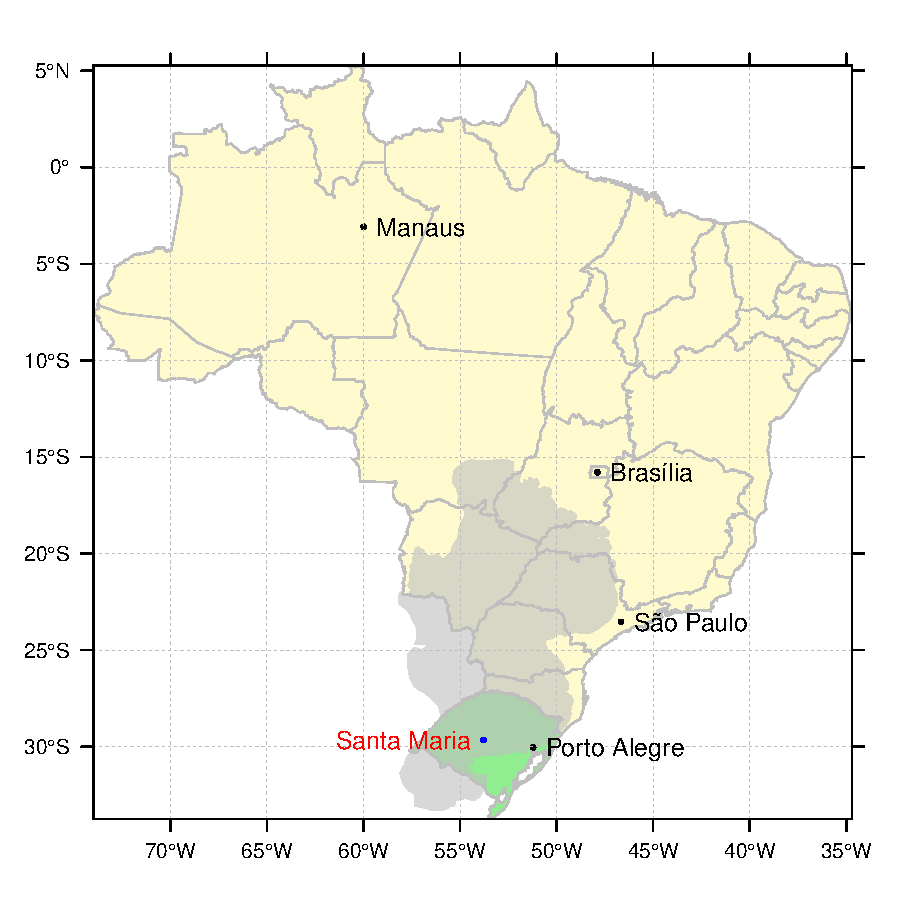
\includegraphics[width=0.90\textwidth]{fig/chap03-location}
\caption[Localização da bacia de captação do reservatório do DNOS-CORSAN, em Santa Maria, RS, 
Brasil]{Localização da bacia de captação do reservatório do Departamento Nacional de Obras de 
Saneamento-Companhia Riograndense de Saneamento no Município de Santa Maria (em vermelho), Estado do Rio 
Grande do Sul (em verde), Brasil, na porção sul da Província Geológica do Paraná (em cinza).}
\label{fig:chap03-location}
\end{figure}

\def\footsolosdors{\footnote{O grupo está registado no Diretório dos Grupos de Pesquisa no Brasil 
(\href{http://dgp.cnpq.br/dgp/espelhogrupo/9373361709890764}{DGP}) mantido pelo CNPq.}}

Os estudos em modelagem espacial do solo na bacia do DNOS -- abreviatura de bacia de captação do reservatório 
do DNOS-CORSAN -- iniciaram no ano de \num{2008} com o grupo de pesquisa \emph{Gênese, composição e 
comportamento dos solos do RS}\footsolosdors{}, sediado no Departamento de Solos da Universidade Federal de 
Santa Maria (\ufsm). Devido à limitação de recursos, o grupo de pesquisa optou por restringir seus estudos em 
modelagem espacial do solo à uma parte da bacia do DNOS. A área escolhida cobre \SI{\pm60}{\percent} de toda a 
bacia do DNOS, o que corresponde à uma área de \SI{\pm18}{\square\kilo\metre}. A área de estudo foi escolhida 
por apresentar acesso facilitado, além de englobar as principais formações geológicas, geoformas, usos da 
terra, e vegetação presentes na bacia do DNOS (\autoref{fig:chap03-perspective}).

\begin{figure}[!ht]
\centering
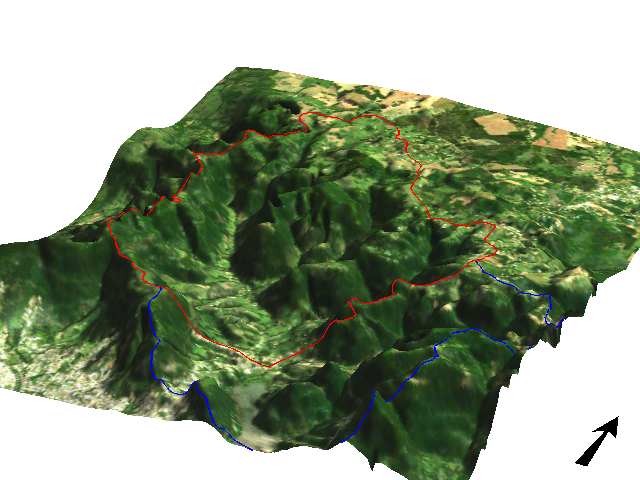
\includegraphics[width = 0.90\textwidth]{fig/chap03-perspective}
\caption[Localização da área de estudo na bacia do DNOS.]{Localização da área de estudo (em vermelho) na 
bacia de captação do reservatório do Departamento Nacional de Obras de Saneamento-Companhia Riograndense de 
Saneamento (DNOS-CORSAN) (em azul). A área de estudo, cujo relevo é bastante acidentado e o uso da terra 
predominante é floresta natural, possui aproximadamente \SI{4}{\km} de largura e \SI{5}{\km} de comprimento, 
o que corresponde a \SI{\pm60}{\percent} da área bacia do DNOS-CORSAN.}
\label{fig:chap03-perspective}
\end{figure}

\section{CLIMA}
\label{sec:chap03-clima}

% Footnote %%%%%
\def\footcfa{\footnote{Mais informações sobre o tipo climático Cfa podem ser encontrados na 
\href{https://pt.wikipedia.org/wiki/Clima_subtropical_\%C3\%BAmido}{Wikipedia}.}}

O clima local é classificado como Cfa\footcfa{} -- subtropical úmido sem estação seca definida --, com 
temperatura média anual de \SI{19,1}{\celsius}. As temperaturas podem alcançar \SI{>40}{\celsius}, no verão, e 
valores negativos no inverno \cite{HeldweinEtAl2009}. A precipitação média anual é de \SI{1708}{\milli\metre} 
bem distribuídos ao longo do ano \cite{Maluf2000}. Predominam os ventos (em ordem de frequência) do quadrante 
leste (frio, úmido e de intensidade fraca a moderada), oeste (frio, seco e de intensidade fraca a moderada) e 
norte (quente, seco e de intensidade moderada a forte) \cite{HeldweinEtAl2009}.

O padrão predominante das chuvas é o avançado, caracterizado por ter seu pico de maior intensidade no início 
da precipitação \cite{MehlEtAl2001}. As chuvas de maior intensidade ocorrem nos meses do final da primavera, 
verão e início do outono \cite{MouraBueno2012}. Como resultado desse padrão, as chuvas de inverno são as 
menos erosivas, mesmo que o conteúdo de água do solo permaneça elevado durante todo o período. O padrão de 
precipitação também é condicionado pelo relevo. Observações feitas em três locais durante o ano de \num{2011}, 
marcado por forte estiagem, mostram variação na lâmina total precipitada entre \num{1317} e \SI{1411}{\mm} 
\cite{MouraBueno2012}. Assim, o relevo plano a montanhoso, com vales encaixados, parece condicionar a formação 
de diferentes regiões microclimáticas, refletindo no volume e intensidade das chuvas \cite{MouraBueno2012}.

O relevo também deve condicionar o fluxo radiativo que atinge as diferentes superfícies. Apesar de não haver 
estudos que demonstrem a efetividade desse fenômeno na área, é reconhecido que grande parte da superfície em 
terrenos de topografia complexa é influenciada pelo efeito de sombreamento, sobretudo nas primeiras horas da 
manhã e no final da tarde \cite{OliphantEtAl2003}. Além disso, a declividade do terreno possui forte 
influência sobre o ângulo de interceptação da radiação solar pelas superfícies \cite{Birkeland1999}. Como 
consequência, deve ocorrer variações na temperatura e conteúdo de água no solo nas diferentes superfícies. Os 
meses de inverno são marcados por ainda menor disponibilidade de radiação solar devido à alta frequência de 
nevoeiros, sobretudo nas partes mais baixas, com valores normais de insolação de \SI{5,1}{\hour\per\day} 
\cite{HeldweinEtAl2009}. Além disso, devido à variação de altitude entre \num{139} e \SI{475}{\metre}, deve 
ocorrer diferença na temperatura da ordem de \SI{4}{\celsius} entre a parte mais baixa e a parte mais alta 
\cite{HeldweinEtAl2009}.

\section{GEOLOGIA}
\label{sec:chap03-geologia}

A geologia é bastante complexa, sendo constituída de três formações geológicas, além de depósitos coluviais 
e aluviais do Quaternário. A literatura sobre o tema é vasta \cite{Bortoluzzi1974, Brasil1980, 
GasparettoEtAl1988, MacielFilho1990, Machado1998, PieriniEtAl2002, MarquesEtAl2005, Milani2005, Pinto2005, 
CPRM2007, Pedron2007, Sartori2009, NascimentoEtAl2010, WerlangEtAl2010, PedronEtAl2012}, e uma revisão da 
mesma é apresentada aqui.

% Link %%%%%
\def\caturrita{\href{https://pt.wikipedia.org/wiki/Forma\%C3\%A7\%C3\%A3o_Caturrita}{Formação Caturrita}}

Na base da sequência estratigráfica, em elevações abaixo de \SI{\pm200}{\metre}, está a \caturrita{}, 
constituída de material sedimentar depositado em ambiente fluvial no Triássico Superior. Sua composição é 
diversa, apresentando seixos de siltito argiloso vermelho na base, seguido de arenito avermelhado de 
granulometria fina à média, composição quartzosa e matriz argilosa, podendo ainda conter considerável teor de 
feldspato, sobreposto por siltito e folhelho também avermelhados. Em geral, a granulometria do arenito é mais 
grosseira e menos argilosa na base da deposição. Devido à sua origem fluvial, a Formação Caturrita apresenta 
marcada estratificação cruzada acanalada e tabular. A origem fluvial também resulta em significativa variação 
espacial na granulometria do arenito, identificada pelo contraste entre áreas de maior cimentação e coesão, 
com outras de maior condutividade hidráulica. Imediatamente acima da Formação Caturrita encontra-se, ora a 
Formação Botucatu, ora a Sequência Inferior da Formação Serra Geral.

% Link %%%%%
\def\serrageral{\href{http://pt.wikipedia.org/wiki/Forma\%C3\%A7\%C3\%A3o_Serra_Geral}{Formação Serra Geral}}

Em elevações entre \num{\pm200} e \SI{\pm350}{\metre} está a Sequência Inferior da \serrageral{} 
(basaltos-andesitos toleíticos). As rochas básicas são de coloração cinza-escura e são constituídas de 
plagioclásio cálcico, clinopiroxênio, magnetita e material intersticial de quartzo e material desvitrificado. 
Em elevações superiores a \SI{\pm350}{\metre} está a Sequência Superior da Formação Serra Geral (vitrófilos, 
riólitos-riodacitos granofíricos). As rochas ácidas apresentam cor cinza-clara, estrutura microcristalina e 
são constituídas de cristais e plagioclásio, clinopiroxênios, hornblenda uralítica e magnetita. A origem 
desse material remonta o Cretáceo, quando sucessivos derrames de lavas de origem vulcânica fissural ocorreram 
durante aproximadamente \num{10} milhões de anos em toda a Bacia do Paraná. Esses eventos ocorreram ao mesmo 
tempo em que iniciava-se a separação das plataformas continentais que hoje constituem a América do Sul e 
África, marcando o final da existência do supercontinente Pangeia.

% Link %%%%%
\def\botucatu{\href{http://pt.wikipedia.org/wiki/Forma\%C3\%A7\%C3\%A3o_Botucatu}{Formação Botucatu}}

O arenito eólico constituinte da \botucatu{} é encontrado tanto assentado sobre a Formação Caturrita, como no 
interior da Formação Serra Geral (arenito \emph{intertrap}). Trata-se de arenito quartzoso de granulometria 
fina à média, contendo feldspato alterado e cimentado por sílica ou por óxido de ferro, que lhe confere a 
coloração rosa-avermelhada. Sua deposição teve início no Cretáceo Inferior, período em que a Bacia do Paraná 
estava sob influência de clima desértico. Essa condição climática continuou durante todo o período em que 
ocorreram as dezenas de eventos de vulcanismo fissural, fazendo com que os mesmos fossem sucedidos por 
deposições eólicas de duração variável. Como a duração e a quantidade de material depositado pelos eventos de 
vulcanismo fissural era variável, assim como o intervalo de tempo entre cada novo evento e a intensidade das 
deposições de sedimentos eólicos, a espessura das camadas do arenito eólico e das rochas vulcânicas é bastante 
variável. Além disso, devido aos diversos eventos de subsidência que ocorreram no eixo central da Bacia do 
Paraná, com consequente soerguimento de suas bordas, as camadas dessas rochas possuem diferentes inclinações 
ao longo de sua faixa de exposição, sendo caracteristicamente ondulada e com suave tendência de inclinação 
para sudoeste.

As deposições do Quaternário são constituídas por depósitos coluviais e aluviais. Em elevações entre 
\num{\pm200} e \SI{\pm300}{\metre} encontram-se depósitos coluviais de material proveniente de uma ou ambas as 
Formações Serra Geral (fragmentos de tamanho variado) e Botucatu. Em elevações abaixo de \SI{\pm200}{\metre} 
são mais comuns os depósitos coluviais de uma ou ambas as Formações Botucatu e Caturrita. Esses depósitos 
ocorrem de maneira descontínua nas encostas. Próximo aos cursos de água na porção mais baixa da bacia e no 
entorno do reservatório, encontram-se depósitos fluviais recentes, geralmente constituídos de fragmentos 
arredondados (seixos) de tamanho variável e/ou sedimentos arenosos. Em pequenas áreas abaciadas e mal 
drenadas, os sedimentos apresentam granulometria mais fina.

\section{GEOMORFOLOGIA}
\label{sec:chap03-geomorfologia}

A área de estudo está situada na porção sul da Bacia Sedimentar do Paraná. Assim, as geoformas atuais são 
resultado dos processos erosivos que ocorreram durante o Terciário e o Quaternário \cite{Sartori2009}, após as 
últimas deposições de lavas vulcânicas e de sedimentos eólicos. Durante esse período, a esculturação da 
paisagem foi determinada pelas alternações entre climas úmidos, semiáridos e áridos \cite{Sartori2009}. 
Atualmente, o clima subtropical úmido favorece a instalação e permanência de vegetação mais eficiente na 
redução do processo de dissecação da paisagem \cite{Sartori2009, NascimentoEtAl2010}. Isso permite que as 
superfícies geomórficas atinjam maior estabilidade e maturidade, embora o uso agrícola das terras tenha 
acelerado, pontualmente, os processos erosivos na área devido à limitada adoção de práticas conservacionistas 
(\autoref{sec:chap03-landuse}).

A bacia do DNOS é abrangida pela unidade morfoestrutural do Rebordo do Planalto da Bacia do Paraná 
\cite{NascimentoEtAl2010}. O Rebordo do Planalto é caracterizado pela ampla variação altimétrica, declividade 
acentuada e escarpas abruptas, apresentando formas denudacionais com topos convexos (fluxo hídrico 
divergente), aguçados e em formas de escarpas. Nesses locais, as vertentes assumem forma retilínea com grande 
desnível \cite{NascimentoEtAl2010}, muitas vezes interrompidas por degraus ou patamares, na maioria das vezes 
encaixadas em falhas e/ou fraturas. Esses patamares são resultado da ação diferencial dos processos 
denudacionais sobre a paisagem, geralmente condicionados pela resistência do material de origem, seja ela 
química/mineralógica (rochas vulcânicas básicas vs. ácidas), física/granulométrica (rochas vulcânicas versus 
sedimentares), ou estrutural (padrão de diaclasamento vertical vs. horizontal das rochas vulcânicas) 
\cite{Holtz2003, Pedron2007, StreckEtAl2008}. Entretanto, em algumas situações, os patamares são formados por 
depósitos coluviais -- mesmo nas partes altas do Rebordo do Planalto -- resultantes de movimentos de massa 
causados por eventos pluviométricos de elevada intensidade e/ou duração \cite{PinheiroEtAl2004, 
PaisaniEtAl2010}. Nesses casos, os patamares possuem menor dimensão e maior declividade. Em outras situações, 
os patamares coluviais, sobretudo aqueles originados dos arenitos da Formação Botucatu, formam 
vertentes alongadas e com menor inclinação, que chegam até a margem dos cursos de água.

Como a bacia do DNOS se encontra em uma região de transição morfoestrutural, as características 
geomorfológicas das porções mais altas e mais baixas da paisagem são similares àquelas encontradas nas 
unidades morfoestruturais adjacentes, respectivamente, o Planalto e a Depressão Periférica. O Planalto é 
marcado pelo relevo suave-ondulado a ondulado, com formas denudacionais de superfícies planas com topos 
convexos (fluxo hídrico divergente). Nesses locais, as vertentes assumem forma convexa levemente ondulada, 
muitas vezes encaixadas em falhas e/ou fraturas \cite{NascimentoEtAl2010}. Já a Depressão Periférica é marcada 
pelo acúmulo de sedimentos provenientes do Planalto e do Rebordo do Planalto, formando planícies aluviais que 
se intercalam entre as coxilhas (denominação regional de colinas). Ali predominam as formas agradacionais de 
planície fluvial e formas denudacionais com topos convexos e superfícies planas. As últimas correspondem às 
coxilhas de algumas dezenas de metros de altitude, geralmente formadas sobre o substrato da Formação Caturrita 
e assentadas na base do Rebordo do Planalto \cite{GasparettoEtAl1988}. Essas coxilhas constituem divisores de 
água de pequena amplitude comumente usados na subdivisão da bacia do DNOS em pequenas sub-bacias 
\cite{Marins2004, Sartori2009}. Nesses locais as vertentes costumam ser alongadas e assumem a forma 
predominantemente côncava devido aos processos de deposição sedimentar e erosão fluvial, muito fracos sob a 
atual condição climática \cite{NascimentoEtAl2010, WerlangEtAl2010}.

A grande heterogeneidade geomorfológica da bacia do DNOS se traduz em uma grande heterogeneidade textural 
do relevo, ou rugosidade, resultante da ação climática ao longo do tempo geológico \cite{NascimentoEtAl2010}. 
Entretanto, em menor escala, a ação antrópica também atuou sobre a configuração geomorfológica da área 
(\autoref{sec:chap03-landuse}). O principal efeito se deu pela erosão da camada superficial do solo, cultivado 
intensivamente sem adoção de práticas conservacionistas ao longo de inúmeras décadas \cite{Menezes2008, 
Sturmer2008, Miguel2010, SamuelRosaEtAl2011a}. Além disso, a abertura de caminhos para acesso às áreas de 
produção nos patamares do Rebordo do Planalto e nos topos de morros proporcionou a formação de canais de 
concentração e escoamento dos fluxos hídricos superficiais, levando à formação inicial de voçorocas. Obras de 
maior expressividade, como ferrovias, ruas e rodovias pavimentadas, conjuntos habitacionais e construções 
isoladas, as quais envolvem operações de terraplanagem e aterramento, também resultaram em modificações 
localizadas na geomorfologia da área. Por fim, a construção do reservatório possibilitou a formação de uma 
área de agradação da paisagem bastante estável em seu entorno, uma vez que o sedimento removido do Planalto e 
do Rebordo do Planalto já não são mais transportados a jusante.

\section{HIDROGRAFIA}
\label{sec:chap03-hidrografia}

A hidrografia da área é condicionada pelas condições geomorfológicas, geológicas, pedológicas e climáticas, ao 
mesmo tempo em que exerce forte influência sobre a modelagem da paisagem \cite{NascimentoEtAl2010}. Como a 
bacia do DNOS é abrangida pela unidade morfoestrutural do Rebordo do Planalto da Bacia do Paraná 
(\autoref{sec:chap03-geomorfologia}), a drenagem apresenta padrão bem definido, geralmente retangular, 
determinado pelas falhas e/ou fraturas \cite{Bortoluzzi1974, GasparettoEtAl1988, NascimentoEtAl2010}. A 
própria formação da bacia do DNOS se deve a existência de falhas e/ou fraturas \cite{GasparettoEtAl1988}. A 
principal e maior delas localiza-se no eixo central da bacia, onde atualmente está localizado o leito do Rio 
Vacacaí-Mirim. Quanto aos tributários do Rio Vacacaí-Mirim, a maioria possui leito assentado sobre outras 
falhas e/ou fraturas de menor dimensão perpendiculares àquela do eixo central da bacia.

Nas áreas mais baixas, cujas características geomorfológicas se assemelham à Depressão Periférica, a drenagem 
apresenta configuração sinuosa, resultado dos processos de deposição sedimentar e erosão fluvial 
\cite{PaivaEtAl2001, SutiliEtAl2009}. Como o relevo é plano a suave-ondulado, e as vertentes longas e 
predominantemente côncavas, o lençol freático fica próximo da superfície do solo. A variação das condições 
meteorológicas ao longo do ano fazem com que o lençol freático apresente flutuação significativa, mantendo o 
conteúdo de água do solo elevado durante os meses mais frios (menor evapotranspiração) 
\cite{HeldweinEtAl2009}. Isso também favorece a ocorrência de inundações, sobretudo nas proximidades dos 
cursos de água e do reservatório \cite{Goldani2006}.

Muitos cursos de água localizados na áreas cujas características geomorfológicas se assemelham ao Planalto, 
assim como no Rebordo do Planalto e nas coxilhas assentadas em sua base, são sazonais. Em geral, esses cursos 
de água estão em atividade apenas nos meses mais frios do ano, quando a disponibilidade de água no ambiente é 
maior, ou durante os eventos de precipitação de forte intensidade, que ocorrem nos meses de verão 
\cite{HeldweinEtAl2009, MouraBueno2012}. Os cursos de água do Rebordo do Planalto costumam apresentar leito 
raso e pedregoso, muitas vezes assentado sobre rochas da Formação Serra Geral \cite{SutiliEtAl2009}. Já os 
cursos de água localizados nos patamares e coxilhas costumam ser rasos, se assentados sobre rochas da Formação 
Caturrita, ou profundos, se assentados sobre rochas da Formação Botucatu ou depósitos coluviais, formando 
voçorocas. Segundo relatos de alguns dos moradores mais antigos da bacia do DNOS, muitas nascentes e pequenos 
cursos de água já perderam totalmente sua atividade, sobretudo quando localizadas no interior ou à jusante de 
áreas de uso antrópico intensivo.

Dado que a declividade e o desnível entre a parte mais baixa e a parte mais alta da área são acentuados, as 
cheias costumam apresentar velocidade e vazão bastante grandes \cite{PaivaEtAl2001, SutiliEtAl2009}. Em média, 
nos \SI{7}{\km} de extensão do Rio Vacacaí-Mirim, da nascente até o reservatório, a declividade média é de 
\SI{0,03}{\m\per\m}. Isso representa um desnível de \SI{\pm210}{\m}, o que resulta em um tempo de concentração 
da bacia estimado de \SI{3}{\hour} \cite{PaivaEtAl2001}. Essas características causam erosão severa nas 
margens dos cursos de água nas áreas mais baixas (depósitos aluviais), sobretudo nos raios externos das 
curvas, onde a velocidade da água é maior \cite{SutiliEtAl2009}. Em alguns trechos, os cursos de água chegaram 
a ter sua largura duplicada em menos de uma década, resultando no aumento da sinuosidade e do nível de fundo 
\cite{PaivaEtAl2001}. Esses eventos comprometem áreas de produção agrícola, bem como a estrutura de 
residências e vias públicas localizadas nas margens dos cursos de água. Grande parte do material removido das 
margens dos cursos de água é transportado para dentro do reservatório, que já perdeu mais de 
um terço de sua capacidade inicial de armazenamento de água \cite{DillEtAl2004}.

\section{USO DA TERRA E VEGETAÇÃO}
\label{sec:chap03-landuse}

A bacia do DNOS foi intensamente ocupada em tempos pretéritos para produção agrossilvopastoril de pequeno 
porte (agricultura familiar) usando sistemas de cultivo convencional com aração periódica e queimada. A grande 
quantidade, extensão e boa distribuição da rede viária em toda a área é uma forte evidência dessa ocupação. A 
área também é cortada por uma estrada férrea e avizinha uma rodovia federal, ambas muito movimentadas. 
Entretanto, nas últimas décadas, muitos caminhos internos das propriedades rurais foram desativados, fruto do 
abandono de muitas áreas de produção agrossilvopastoril, a maioria delas localizada nos topos dos morros, 
patamares do Rebordo ou no fundo de vales, onde a manutenção dos caminhos é muito onerosa, especialmente 
quando distantes da sede das propriedades (\autoref{fig:chap05-land-use} e \autoref{fig:chap05-sat-image}). No 
passado, essas estradas internas possibilitavam o trânsito de pessoas e o transporte da produção 
agrossilvopastoril, a qual era usa para suprir as necessidades próprias, sendo o excedente comercializado às 
margens da estrada férrea e nas áreas urbanas do município. Atualmente, o tráfego existente está concentrado 
nas estradas principais e secundárias, enquanto alguns poucos caminhos internos ainda são utilizados para 
condução de rebanhos ou acesso a pequenas áreas de produção agrossilvopastoril. A maioria dos caminhos internos 
inativos está localizada no interior de áreas de floresta natural regenerada, o que dificulta a sua 
identificação com imagens aéreas ou orbitais. Em alguns casos, esses caminhos são utilizados em atividades de 
turismo, especialmente para caminhadas a pé, ou atividades esportivas com motocicletas (trilhas).

O abandono de muitas áreas de produção agrossilvopastoril possibilitou a regeneração da vegetação natural em 
grande parte da bacia do DNOS. Atualmente, a área ocupada por florestas e vegetação secundária (capoeira) 
representa \SI{\pm60}{\percent} da área total \cite{SamuelRosaEtAl2011a}. Isso mostra que, assim como toda a 
região do Rebordo do Planalto da Bacia do Paraná, o uso da terra para fins agrossilvopastoris na bacia do DNOS 
também foi desintensificado nas últimas décadas \cite{SEMA/UFSM2001, DillEtAl2004, Poelking2007, Miguel2010, 
SamuelRosaEtAl2011a, Dullius2012, TenCatenEtAl2012}. As áreas de floresta são encontradas nos mais diversos 
estádios de desenvolvimento, com os estratos intermediário e superior concentrando a maior parte dos 
indivíduos. As florestas originais, e secundárias em estádio avançado de desenvolvimento, são encontradas, 
predominantemente, em áreas de difícil acesso. Em geral, as áreas de floresta predominam nas regiões com maior 
declividade e solo raso e pedregoso. Tais condições pedológicas são resultado das condições geológicas e 
geomorfológicas e/ou da degradação causada pelo intenso uso da terra para produção agrossilvopastoril durante 
inúmeras décadas usando sistemas de cultivo convencional \cite{SamuelRosaEtAl2011a}.

A ocorrência de fragmentos florestais ao longo das margens dos cursos de água, estradas e próximo de 
edificações é comum. Nas formações mais jovens, é comum encontrar fragmentos de carvão e outros sinais do uso 
agrossilvopastoril num passado recente. As áreas sob vegetação secundária (capoeira) também ocorrem em toda a 
bacia do DNOS, predominantemente em locais de difícil acesso e acentuada declividade, geralmente interligados 
por caminhos internos, indicando sua utilização agrossilvopastoril no passado \cite{SamuelRosaEtAl2011a}. Sua 
composição florística varia entre as áreas, predominando espécies de porte herbáceo e arbustivo. O solo dessas 
áreas costuma ser menos pedregoso que nas áreas florestadas, mas apresentam profundidade semelhante 
\cite{SamuelRosaEtAl2011a}, possivelmente indicando que as atividades agrossilvopastoril foram encerradas 
antes do solo atingir seu nível máximo de degradação. Entretanto, a reserva de nutrientes do solo, assim como 
a sua fertilidade física, foram esgotadas a tal ponto que a vegetação secundária ainda não foi capaz de 
produzir melhorias significativas quando comparado com as condições originais \cite{Menezes2008, 
Zalamena2008}.

Apesar do abandono de muitas áreas de produção agrossilvopastoril nas últimas décadas, sobretudo aquelas com 
maior dificuldade de acesso, os caminhos internos utilizados para o escoamento da produção, mesmo depois de 
inativos, continuam associados ao processo de degradação do solo. Isso ocorre porque, na grande maioria dos 
casos, todo o fluxo da água de escoamento superficial proveniente dos eventos de precipitação é concentrado 
nesses caminhos internos, onde, geralmente, quantidade significativa de resíduos vegetais está depositada. 
Esse resíduo vegetal, mais a fração mineral do solo carregada pela enxurrada, costuma chegar com facilidade 
aos cursos de água. No caso dos caminhos internos ainda utilizados na condução de rebanhos bovinos, a produção 
de sedimentos minerais tende a ser ainda maior, haja vista o impacto mecânico do pisoteio animal sobre a 
desagregação do solo. Além disso, muitas áreas florestadas e sob vegetação secundária ainda são utilizadas 
para o pastoreio de bovinos e equinos \cite{SamuelRosaEtAl2011a}. Isso causa a degradação da camada 
superficial do solo, sobretudo pela sua compactação, dificultando a infiltração da água dos eventos de 
precipitação, o que resulta na perda da serapilheira \cite{ScheneiderEtAl1978}. Além disso, a própria 
regeneração natural é prejudicada, uma vez que plantas em estádio inicial de desenvolvimento e raízes 
superficiais são destruídas \cite{ScheneiderEtAl1978, HackEtAl2005}. O resultado desse processo é a redução da 
capacidade do solo em suportar o desenvolvimento potencial da floresta \cite{KonigEtAl2002}.

Dado que a bacia do DNOS também possui áreas com relevo plano a suave-ondulado e solo profundo, 
\SI{\pm30}{\percent} de sua superfície ainda é utilizada com atividades agrossilvopastoris ao longo de todo o 
ano, principalmente a pecuária bovina extensiva \cite{SamuelRosaEtAl2011a}. As áreas de produção animal 
extensiva predominam nas porções norte, sul e centro-oeste, ao longo dos cursos de água e estradas. O solo é 
mais profundo e menos pedregoso do que em áreas de floresta natural e vegetação secundária. É comum encontrar 
fragmentos de carvão e formações de microrrelevo devido ao uso de implementos agrícolas para o revolvimento do 
solo na maior parte desses locais, evidenciando seu uso agrícola num passado recente. Essas áreas podem ser 
divididas entre aquelas de campo sujo (pastagens naturais mal manejadas, com predomínio de vegetação de porte 
herbáceo-arbustivo) e campo limpo (pastagens naturais e perenes bem manejadas) \cite{SamuelRosaEtAl2011a}. Em 
geral, as áreas de campo sujo estão próximas a áreas de vegetação secundária (capoeira), com relevo mais 
declivoso e solo mais pedregoso e raso do que aquelas de campo limpo. Assim como nas áreas de floresta e sob 
vegetação secundária, a dinâmica de uso dessas áreas ao longo do tempo é bastante complexa, dificultando o 
estabelecimento de relações diretas com a maior parte das características do solo. Entretanto, sob o ponto de 
vista da reserva de nutrientes e matéria orgânica, o solo pode ser considerado pobre, uma vez que a exploração 
pecuária é totalmente extrativista e extensiva.

As atividades agrossilvopastoris que ocupam menor extensão territorial são a agricultura e a silvicultura. As 
áreas de lavoura anuais e bianuais estão dispersas em toda a área, geralmente localizadas em terrenos de 
menor declividade e solo medianamente profundo. Entretanto, algumas áreas de produção agrícola possuem 
declives superiores a \SI{50}{\percent} e solo raso e pedregoso \cite{SamuelRosaEtAl2011a}. Em qualquer das 
situações, as condições de degradação do solo costumam ser bastante avançadas devido ao emprego de sistemas 
convencionais de cultivo, exceto por algumas áreas de produção olerícola. As florestas plantadas 
(\textit{Eucalyptus spp.}) são implantadas em áreas com menor declividade e solo mais profundo, geralmente 
onde o acesso com máquinas é melhor, sobretudo pela necessidade de manejo e escoamento da produção. A área 
ocupada por essa atividade possui tendência de crescimento, haja vista os novos plantios existentes e o relato 
de alguns moradores \cite{SamuelRosaEtAl2011a}. Em geral, os novos plantios são implantados em áreas de 
produção agropecuária, seja pelo elevado nível de degradação do solo já atingido, seja pela redução da força 
de trabalho das famílias devido ao êxodo rural, ou pela maior lucratividade dessa atividade.

Por fim, as obras de engenharia e assentamentos urbanos são aquelas que ocupam a menor parte da bacia do DNOS. 
No que diz respeito à malha viária, a maior concentração ocorre na porção sul, junto ao maior assentamento 
urbano, localizado no entorno do reservatório. Entretanto, diversas construções são encontradas ao longo das 
estradas que cortam a área, muitas das quais são pertencentes a moradores do centro da cidade de Santa Maria e 
são utilizadas apenas como sítios de final de semana. O número de sítios de final de semana aumentou 
significativamente nas últimas décadas \cite{Goldani2006}, muitos dos quais construídos em locais 
inapropriados, como margens dos corpos de água e áreas com forte declividade. Esse processo de urbanização 
desordenada, que exigiu a realização de obras de corte e aterramento dos terrenos, é um importante 
contribuinte da carga de sedimentos recebida pelo reservatório anualmente, aos quais somam-se os resíduos 
domésticos e cloacais \cite{Goldani2006, PaivaEtAl2001, DillEtAl2004, MiguelEtAl2014}. Quanto às demais obras 
de engenharia, destacam-se os reservatórios de água, a maioria deles de pequena extensão, utilizados para a 
dessedentação animal. Como os cursos de água de maior volume estão localizados na porção sul da área, a maior 
parte dos reservatórios de água está na porção norte \cite{SamuelRosaEtAl2011a}. Além disso, a menor 
permeabilidade do solo e do substrato rochoso, bem como da condição topográfica, favorecem essa 
característica.

\section{PEDOLOGIA}

O solo da bacia do DNOS possui características com forte dependência do material de origem que, conforme 
descrito anteriormente, é um importante condicionante da geomorfologia e da hidrografia 
\cite{NascimentoEtAl2010}. Nas superfícies geomórficas mais estáveis, como no topo do Planalto (rochas 
vulcânicas), nos terraços do Rebordo (rochas vulcânicas e sedimentares) e nas coxilhas de relevo 
suave-ondulado a ondulado (rochas sedimentares), as condições ambientais são mais favoráveis ao 
desenvolvimento do solo em profundidade \cite{Moser1990}. O contrário ocorre nas áreas de relevo mais 
acidentado do Rebordo, onde acredita-se que a taxa de formação do solo seja semelhante à taxa de remoção 
natural \cite{Moser1990, DalmolinEtAl2006a, Sturmer2008, SamuelRosaEtAl2011a}. Além da condição 
geomorfológica, a resistência da rocha ao intemperismo também condiciona o desenvolvimento do solo em 
profundidade nesses locais \cite{Pedron2007}. Já nas planícies aluviais, as características do solo foram 
fortemente influenciadas pelo hidromorfismo e deposição sedimentar, geralmente resultando em solo de coloração 
acinzentada e maior profundidade do que nas área declivosas Rebordo \cite{Moser1990, Miguel2010}. A forte 
influência da geologia também aparece na textura do solo (\autoref{fig:chap03-clay-land-parent}). Enquanto os 
arenitos conferem textura arenosa ao solo, sobretudo aqueles da Formação Botucatu, as rochas vulcânicas 
conferem textura média ao solo, sobretudo os basaltos-andesitos toleíticos (\autoref{sec:chap05-geo-maps}).

\begin{figure}[!ht]
\centering
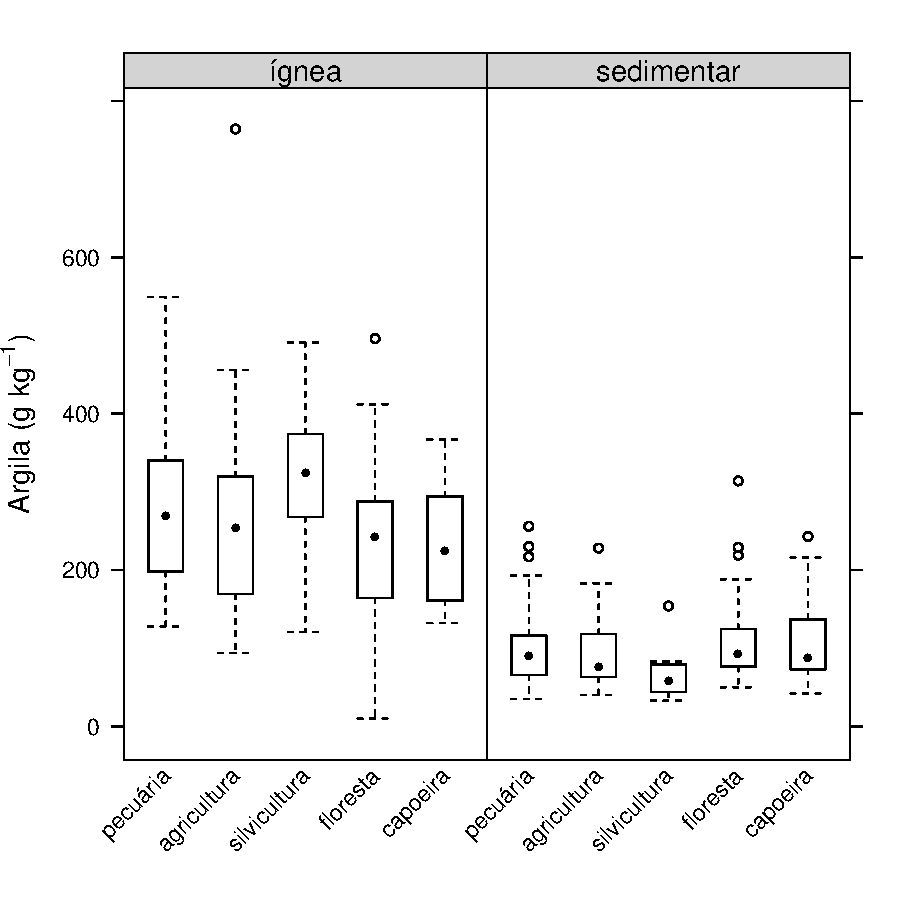
\includegraphics[width=0.60\textwidth]{fig/chap03-clay-land-parent}
\caption[Argila no solo e sua relação com o uso da terra e o material de origem do solo.]{
Distribuição do conteúdo de argila (\si{\gram\per\kilo\gram}) na camada superficial do solo (\SI{\leq20}{\cm}) 
e sua relação com o uso da terra e vegetação (pecuária, agricultura, silvicultura, floresta e capoeira) e o 
tipo de material de origem (ígnea -- rocha ígnea, ou sedimentar -- rocha sedimentar ou sedimentos diversos).
Solo desenvolvido a partir de material de origem sedimentar costuma apresentas conteúdo de argila inferior à 
solo desenvolvido a partir de material de origem ígnea. Em geral, essa relação é pouco influenciada pelo tipo 
de uso da terra. A exceção são as áreas destinadas à silvicultura localizadas no setor norte da bacia do DNOS, 
cujo solo desenvolveu a partir de material de origem ígnea. Ali a tendência é de o solo apresentar maior 
conteúdo de argila na camada superficial.}
\label{fig:chap03-clay-land-parent}
\end{figure}

Como a bacia do DNOS possui a maior parte de sua área em condições de declividade moderada à forte, e foi 
intensamente ocupada em tempos pretéritos para produção agrossilvopastoril com aração e queimada periódicas 
(\autoref{sec:chap03-landuse}), o solo é, predominantemente, pouco profundo. Nas áreas de declividade moderada 
à forte o solo costuma apresentar profundidade inferior à \SI{50}{\cm} até o contato lítico, sendo comum a 
ocorrência de pedregosidade e rochosidade abundantes \cite{Miguel2010}. Assim, predominam as classes 
taxonômicas Neossolo Litólico Distro-Úmbrico típico, Cambissolo Háplico Ta Eutrófico típico, Neossolo Litólico 
Eutro-Úmbrico típico e Neossolo Regolítico Distro-Úmbrico típico (\autoref{sec:chap05-soil-maps}). O efeito do 
uso inapropriado do solo para produção agrossilvopastoril aparece mesmo em algumas áreas de maior estabilidade
(topos de morros, patamares do Rebordo do Planalto e coxilhas) onde as condições para o desenvolvimento 
pedogenético são mais favoráveis \cite{Moser1990, MouraBueno2012}. Por exemplo, alguns patamares do Rebordo, 
inicialmente constituídos de colúvios sedimentares (arenito Botucatu) e vulcânicos (fragmentos de tamanhos 
variáveis), apresentam solo com superfície recoberta por fragmentos rochosos, fruto da forte erosão a que foi 
submetido, limitando a continuação de seu uso para atividades agrossilvopastoris \cite{MouraBueno2012}. Essas 
atividades também resultaram na depleção da fertilidade do solo, marcada atualmente pelos baixos conteúdo de 
carbono orgânico (\autoref{fig:chap03-orca-land-parent}) e capacidade de troca de cátions efetiva 
(\autoref{fig:chap03-ecec-land-parent}).

\begin{figure}[!ht]
\centering
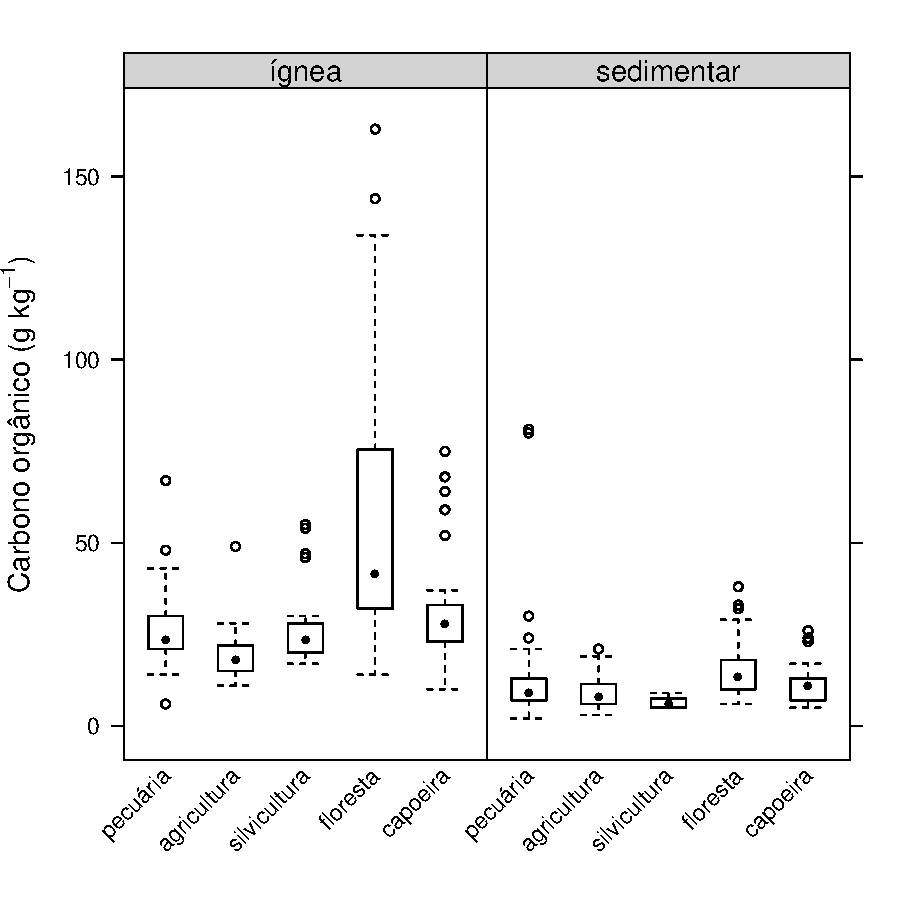
\includegraphics[width=0.60\textwidth]{fig/chap03-orca-land-parent}
\caption[Carbono orgânico no solo e sua relação com o uso da terra e o material de origem do solo.]{
Distribuição do conteúdo de carbono orgânico (\si{\gram\per\kilo\gram}) na camada superficial do solo 
(\SI{\leq20}{\cm}) e sua relação com o uso da terra e vegetação (pecuária, agricultura, silvicultura, floresta 
e capoeira) e o tipo de material de origem (ígnea -- rocha ígnea, ou sedimentar -- rocha sedimentar ou 
sedimentos diversos). O conteúdo de carbono é mais elevado em solo florestal, independente do tipo de rocha 
que deu origem ao solo. Contudo, o conteúdo de carbono é notadamente maior quando o solo tem rocha ígnea como 
material originário, sugerindo uma íntima relação com o conteúdo de argila do solo 
(\autoref{fig:chap03-clay-land-parent}) e de cátions básicos liberados durante o intemperismo do material de 
origem, refletido na capacidade de troca de cátions efetiva do solo (\autoref{fig:chap03-ecec-land-parent}). A 
grande variação no conteúdo de carbono em solo florestal reflete a ocorrência de vários estágios de sucessão 
florestal.}
\label{fig:chap03-orca-land-parent}
\end{figure}

Existe consenso de que a pequena profundidade do solo na maior parte da bacia do DNOS seja devida ao material 
de origem, às condições geomorfológicas e hidrológicas, bem como aos sistemas de cultivo do solo empregados ao 
longo de inúmeras décadas. Contudo, a diversidade de fatores e a escassez de estudos torna impossível isolar a 
contribuição individual de cada fator. Por exemplo, não existe estimativa quantitativa do volume total de solo 
perdido devido à erosão em áreas de produção agrossilvopastoril. Entretanto, acredita-se que horizontes 
pedogenéticos inteiros tenham sido removidos, dando origem ao processo de retrocesso pedogenético do solo
\cite{SamuelRosaEtAl2011a}. Esse processo reflete a involução da classificação taxonômica do solo dentro de um 
determinado sistema taxonômico. A comum ocorrência do táxon Neossolo Litólico com solum de pouco menos de 
\SI{50}{\cm} em inúmeras áreas de produção agrícola é usada para corroborar essa hipótese. Isso porque o valor 
de \SI{50}{\cm} para o solum é aquele usado para distinguir os taxa Neossolo Litólico e Neossolo Regolítico no 
Sistema Brasileiro de Classificação do Solo \cite{SantosEtAl2013a}. A mesma hipótese foi levantada em outras 
regiões de topografia complexa para explicar a identificação dos táxa Cambissolo e Luvissolo onde antes 
observava-se o táxon Chernossolo \cite{StreckEtAl2008}. Essa involução da classificação taxonômica seria 
resultado da remoção do horizonte pedogenético A chernozêmico devido à erosão acelerada pelo uso agrícola 
extrativista e intenso praticado por várias décadas. Em resumo, nas áreas onde a taxa de formação do solo é 
semelhante à taxa de erosão natural, o uso agrossilvopastoril da terra sem adoção de práticas 
conservacionistas invariavelmente resultaria na degradação do solo e consequente retrocesso pedogenético 
porque a soma das taxas de erosão natural e erosão induzida seria maior do que a taxa de formação do solo.

\begin{figure}[!ht]
\centering
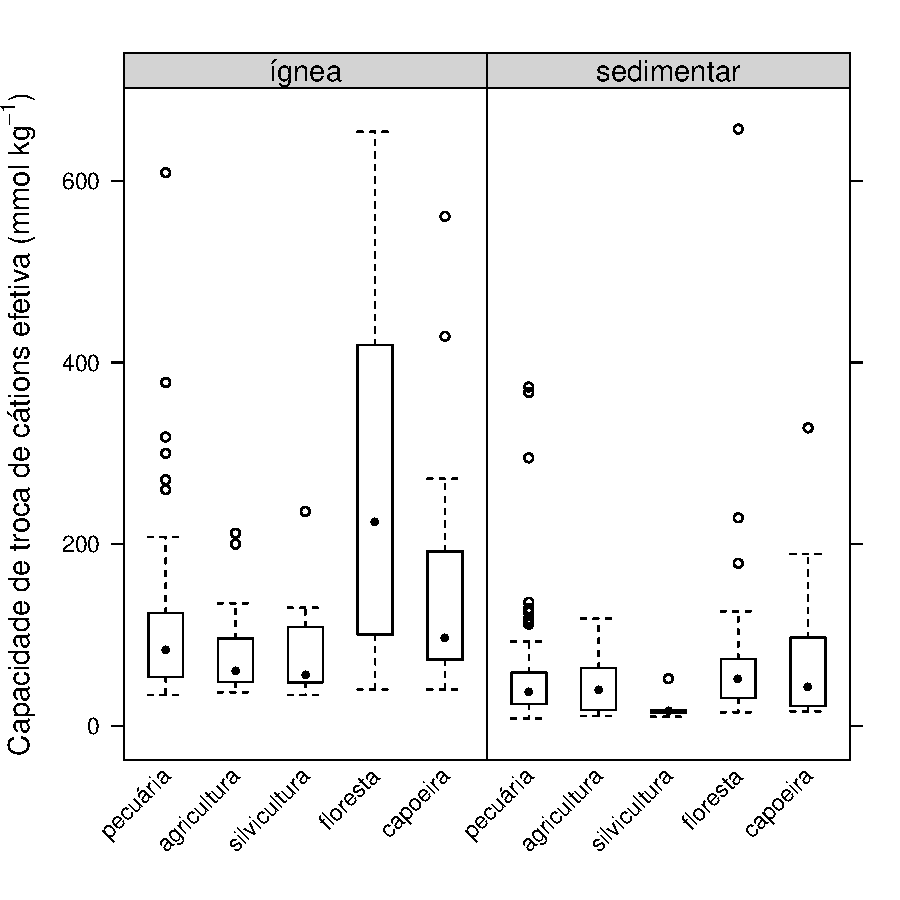
\includegraphics[width=0.60\textwidth]{fig/chap03-ecec-land-parent}
\caption[Capacidade de troca de cátions efetiva no solo e sua relação com o uso da terra e o material de 
origem do solo.]{Distribuição da capacidade de troca de cátions efetiva (\si{\milli\mole\per\kilo\gram}) na 
camada superficial do solo (\SI{\leq20}{\cm}) e sua relação 
com o uso da terra e vegetação (pecuária, agricultura, silvicultura, floresta e capoeira) e o tipo de material 
de origem (ígnea -- rocha ígnea, ou sedimentar -- rocha sedimentar ou sedimentos diversos).}
\label{fig:chap03-ecec-land-parent}
\end{figure}

As áreas com maior potencial de desenvolvimento pedogenético em profundidade possuem menor expressão 
territorial. Elas correspondem à paisagem menos declivosa do Planalto (rochas vulcânicas), algumas coxilhas 
(rochas sedimentares) e depósitos aluviais \cite{Miguel2010}. Em áreas de material de origem vulcânica, 
sobretudo basaltos-andesitos toleíticos, identifica-se o táxon Argissolo Vermelho Alítico típico, que 
caracteriza solo com horizonte superficial de textura arenosa a média, sobrejacente a um horizonte 
subsuperficial de textura média a argilosa \cite{Miguel2010}. Nas áreas do Planalto em que ocorrem 
riólitos-riodacitos granofíricos, o solo costuma apresentar menor profundidade, sendo predominantemente 
classificado como Neossolo Litólico e Cambissolo Háplico. Em pequenas manchas, o solo é classificado como 
Argissolo Vermelho-Amarelo. O menor desenvolvimento do solo em profundidade em área de riólitos-riodacitos 
granofíricos deve-se, em parte, à maior resistência dessas rochas ao intemperismo, uma vez que possui maior 
teor de sílica, sobretudo na forma de grandes de cristais de quartzo cristalizados a baixa temperatura 
(\SI{<600}{\celsius}) \cite{Pedron2007}. Contudo, a pequena profundidade do solo também resulta da degradação 
causada pelo longo uso agrossilvopastoril sem adoção de práticas conservacionistas. Até o momento é impossível 
isolar a contribuição desses dois fatores de formação sobre as características do solo.

Em áreas de material de origem sedimentar (Formação Caturrita), o solo costuma ser classificado como 
Argissolo Bruno-Acinzentado Alítico abrúptico. Trata-se de solo com horizonte superficial de textura arenosa 
que transiciona de maneira abrupta para um horizonte subsuperficial de textura argilosa \cite{Miguel2010}. 
Essa descontinuidade textural geralmente é atribuída a processos pedogenéticos, sobretudo a perda (erosão 
lateral seletiva) e translocação (argiluviação) das partículas mais finas. Contudo, devido à complexidade 
geológica e geomorfológica da área, outros fatores podem ter contribuído. O primeiro deles estaria relacionado 
às características do próprio material de origem que, por ter sido formado em ambiente fluvial durante um 
período de mudança climática no Triássico, apresenta camadas deposicionais com granulometria diferenciada 
\cite{PieriniEtAl2002}. Assim, a presença de camadas de siltitos e folhelhos poderia ter contribuído para a 
formação da descontinuidade textural. Outro fator seria uma possível contribuição dos arenitos da Formação 
Botucatu e \emph{intertrap} na Formação Serra Geral. Dado que esse material está localizado em posições 
superiores na paisagem e são bastante suscetíveis à erosão, o mesmo poderia ter contribuído para a formação do 
horizonte superficial arenoso do solo. Em ambos os casos, a descontinuidade textural seria atribuída à 
ocorrência de descontinuidade litológica, com a diferença de que no primeiro caso as litologias pertenceriam à 
mesma formação geológica.

Nas áreas deprimidas da paisagem do Planalto, formando pequenas bacias de acumulação, ou nas áreas planas ao 
longo dos cursos de água da Depressão Periférica, o solo é classificado como Planossolo Háplico Alítico típico 
\cite{Miguel2010}. Trata-se de solo com horizonte superficial de textura média sobre horizonte subsuperficial 
de textura média a argilosa, podendo ou não apresentar horizonte intermediário eluvial. Ainda mais próximo dos 
cursos de água, o solo é classificado como Neossolo Flúvico Tb Eutrófico fragmentário \cite{Miguel2010}. Como 
o seu material de origem é diverso e possui arranjamento espacial discordante, a textura do solo é variável, 
mas sempre arenosa ou média, nunca argilosa, mesmo quando presente em áreas do Planalto ou do Rebordo. Por 
fim, com expressão territorial ainda menor, o solo é classificado como Neossolo Quartzarênico Órtico típico em 
alguns patamares do Rebordo, sejam eles de origem estrutural ou da deposição de colúvios do arenito da 
Formação Botucatu.

Atualmente, o aumento da área ocupada por florestas devido ao abandono de diversas área de produção sugere que 
a bacia do DNOS esteja adentrando um período de redução da degradação do solo, exceto nas áreas de expansão 
urbana. Os processos erosivos já apresentam caráter mais pontual, onde a geomorfologia parece possuir papel 
preponderante. Segundo estimativas, apenas uma pequena fração da área apresenta perdas de solo por erosão 
laminar acima de valores toleráveis \cite{Miguel2010}. Algumas observações até mesmo indicam que essas 
estimativas estão acima da perda real de solo por erosão laminar \cite{MouraBueno2012}.


Espera-se que a redução da degradação do solo contribua, num futuro próximo, para a construção de um 
entendimento mais acurado da relação entre o solo e os demais componentes ambientais, principalmente nas áreas 
florestadas recentemente abandonadas.
 % 3. Modelo conceitual de pedogênese
\selectlanguage{english}
% \artigotrue
\chapter{THE SANTA MARIA DATASET. PART I -- SOIL DATA}
\chapternote{Collaborated in the preparation of this manuscript: Pablo Miguel (UFPel), Jean Michel Moura Bueno 
(UFSM), Ricardo Simão Diniz Dalmolin (UFSM), Andrisa Balbinot (UFSM), Lúcia Helena Cunha dos Anjos (UFRRJ), 
Gustavo de Mattos Vasques (Embrapa Solos), Gerard B. M. Heuvelink (ISRIC -- World Soil Information), and Ad 
van Oostrum (ISRIC -- World Soil Information).}
\shorttitle{Soil Data}
\label{chap:chap04}
%\SweaveUTF8


%\def\ptkeys{}
%\begin{chapterabstract}{brazilian}{\ptkeys}
% Este é o resumo em português.
%\end{chapterabstract}

\def\enkeys{Spatial soil modelling. Purposive sampling. Legacy data. Soil field description. Soil laboratory 
analysis}
  
\begin{chapterabstract}{english}{\enkeys}
The Santa Maria dataset comprises soil data from $n = 410$ point soil observations made between \num{2008} and 
\num{2013} in the catchment of the reservoir of the \textit{Departamento Nacional de Obras de 
Saneamento}-\textit{Companhia Riograndense de Saneamento} (DNOS-CORSAN), located in the southern Brazilian 
state of Rio Grande do Sul. These soil data were produced during the development of research projects that 
aimed at producing semi-detailed soil and land use maps, and predicting topsoil carbon stock and vulnerability 
to erosion. All observation locations were selected purposively or by convenience. Several environmental 
features were described at the observation locations, such as land use, geology, soil classification, slope, 
drainage condition, presence of coarse fragments and rock outcrops, soil coverage with vegetation, among 
other peculiarities of each observation location that were not recorded in a systematic way. Soil samples were 
submitted to laboratory analysis to determine the soil organic carbon content, particle size distribution, 
bulk density, and the content of exchangeable bases (calcium, magnesium, potassium, and sodium) and acidity. 
The effective cation exchange capacity was calculated as the sum of exchangeable bases and acidity. The soil 
data is freely available in a repository hosted in GitHub. These include the identification of all observation 
locations, their geographic coordinates, and field and laboratory data. The number of laboratory replicates 
and the sample standard deviation is provided as well.
\end{chapterabstract}

\formatchapter

\section{INTRODUCTION}
\label{sec:chap04-introduction}

The Santa Maria dataset comprises soil data from $n = 410$ point soil observations made between \num{2004} and 
\num{2013} in the catchment of the reservoir of the \textit{Departamento Nacional de Obras de 
Saneamento}-\textit{Companhia Riograndense de Saneamento} (DNOS-CORSAN), located in the southern border of the 
Plateau of the Paraná Sedimentary Basin, in the city of Santa Maria, state of Rio Grande do Sul, Brazil. These 
point soil observations cover the northern sector of the catchment -- an area of \SI{\pm2000}{\hectare}, which 
corresponds to \SI{\pm60}{\percent} of the entire catchment. These soil data were produced during the 
development of research projects that aimed at producing semi-detailed soil and land use maps (\scale{25000}) 
\cite{Pedron2005, Miguel2010, SamuelRosaEtAl2011a, MiguelEtAl2012}, and predicting topsoil carbon stock and 
vulnerability to erosion \cite{Samuel-Rosa2009, MouraBueno2012, Miguel2013}.

This manuscript presents a description of the soil data contained in the Santa Maria dataset, including the 
procedures for soil sampling and description, as well as the analytical methods employed. The soil data is 
freely available as comma-separated values (CSV) files in a repository hosted in \dnosgeneral{}. Files 
\texttt{fieldData.csv} and \texttt{labData.csv} contain the identification of all observation locations, their 
geographic coordinates (latlong, WGS1984), and field and laboratory data, respectively. Files 
\texttt{fieldMetadata.csv} and \texttt{labMetadata.csv} contain the metadata. Every soil property is 
identified with a code composed of three or four capital letters. For example, soil organic carbon is 
identified with \texttt{ORCA}. A column containing the number of laboratory replicates is identified with the 
code of the soil property followed by the letter \q{N}. The column containing the sample standard deviation is 
identified in the same manner, but using \q{SD}. For example, \texttt{ORCA\_N} and \texttt{ORCA\_SD}.

The reader should be aware that soil science evolved in Brazil following a somewhat different pathway than in 
the countries of the northern hemisphere due to the specific soil features of tropical and subtropical 
regions. Methods have been adapted along the years, possibly leading to nomenclature mismatches. The reader is 
invited to contribute to solve any problems in this document.

\section{FIELD SAMPLING}
\label{sec:chap04-sampling}

The Santa Maria dataset is composed of three subsets which are described in the next three sections. Together, 
these subsets yield a sampling density of about \num{\pm0.18}~observations per hectare, with an average 
separation distance between two neighbouring points of \SI{180}{\metre}, minimum and maximum separation 
distances of \num{18} and \SI{328}{\metre}, \SI{95}{\percent} of neighbouring observations being separated by 
more than \SI{49}{\metre}.

\subsection{Subset I}

The first subset ($n = 340$, \autoref{fig:chap04-subsets-I-III}) was produced as part of projects that aimed 
at producing semi-detailed soil and land use maps, and predicting topsoil carbon stock and vulnerability to 
erosion \cite{Samuel-Rosa2009, SamuelRosaEtAl2011a, MiguelEtAl2012, Moura-BuenoEtAl2012, Samuel-RosaEtAl2013}. 
The researchers faced several difficulties with a budget cut and shortage of workforce. They also had 
restricted access to several areas due to geographic barriers and prohibition of access by some landowners. 
These difficulties forced the researchers to reduce the originally aimed number of observations ($n = 500$) 
during the development of the project.

\def\foottacit{\footnote{A comprehensive explanation of what \emph{tacit knowledge} is, opposed to explicit 
knowledge, can be found in \href{https://en.wikipedia.org/wiki/Tacit_knowledge}{Wikipedia}.}}

All observation locations were selected purposively or by convenience. Tacit knowledge\foottacit{} was the 
main tool to choose the observation locations, a process that was carried out in the office using 
\googleearth{} imagery of the years of \num{2008} and \num{2009}. The main goal of the researchers was to 
obtain a sample that they understood as being representative of the different landforms, land uses, and soil 
taxa present in the study area. They also wanted the observations to be spread throughout the entire study 
area.

At the observation locations, the researchers defined an area of \SI{\pm100}{\metre\squared} within which they 
opened three soil pits up to a depth of \SI{20}{\centi\metre}. Soil samples were collected up to a depth of 
\SI{20}{\centi\metre}, the depth being measured with a ruler. The resulting sampling depth of Subset I varies 
from \num{2} to \SI{20}{\centi\metre}, with an average of \SI{17}{\centi\metre}. This variation of the 
vertical sampling support was not a problem for the researchers because their goal was to sample the 
\emph{topsoil}. The topsoil was defined as the topmost soil layer, with a thickness equal or inferior to 
\SI{20}{\centi\metre}, being the soil layer most susceptible to degradation induced by poor agricultural 
practices and land use changes.

Soil samples from the three pits opened in each sampling area were used to produce a composite sample which 
was used for laboratory analyses. Subsurface soil features were observed with an auger in each pit, and the 
average (continuous variables) or most common (categorical variables) value recorded. Note that soil sampling 
was done using an areal support -- an area of \SI{\pm100}{\metre\squared}. However, the shape and exact area of 
the sampling units are unknown, and georeferencing took place at point support.

\begin{figure}[!ht]
\centering
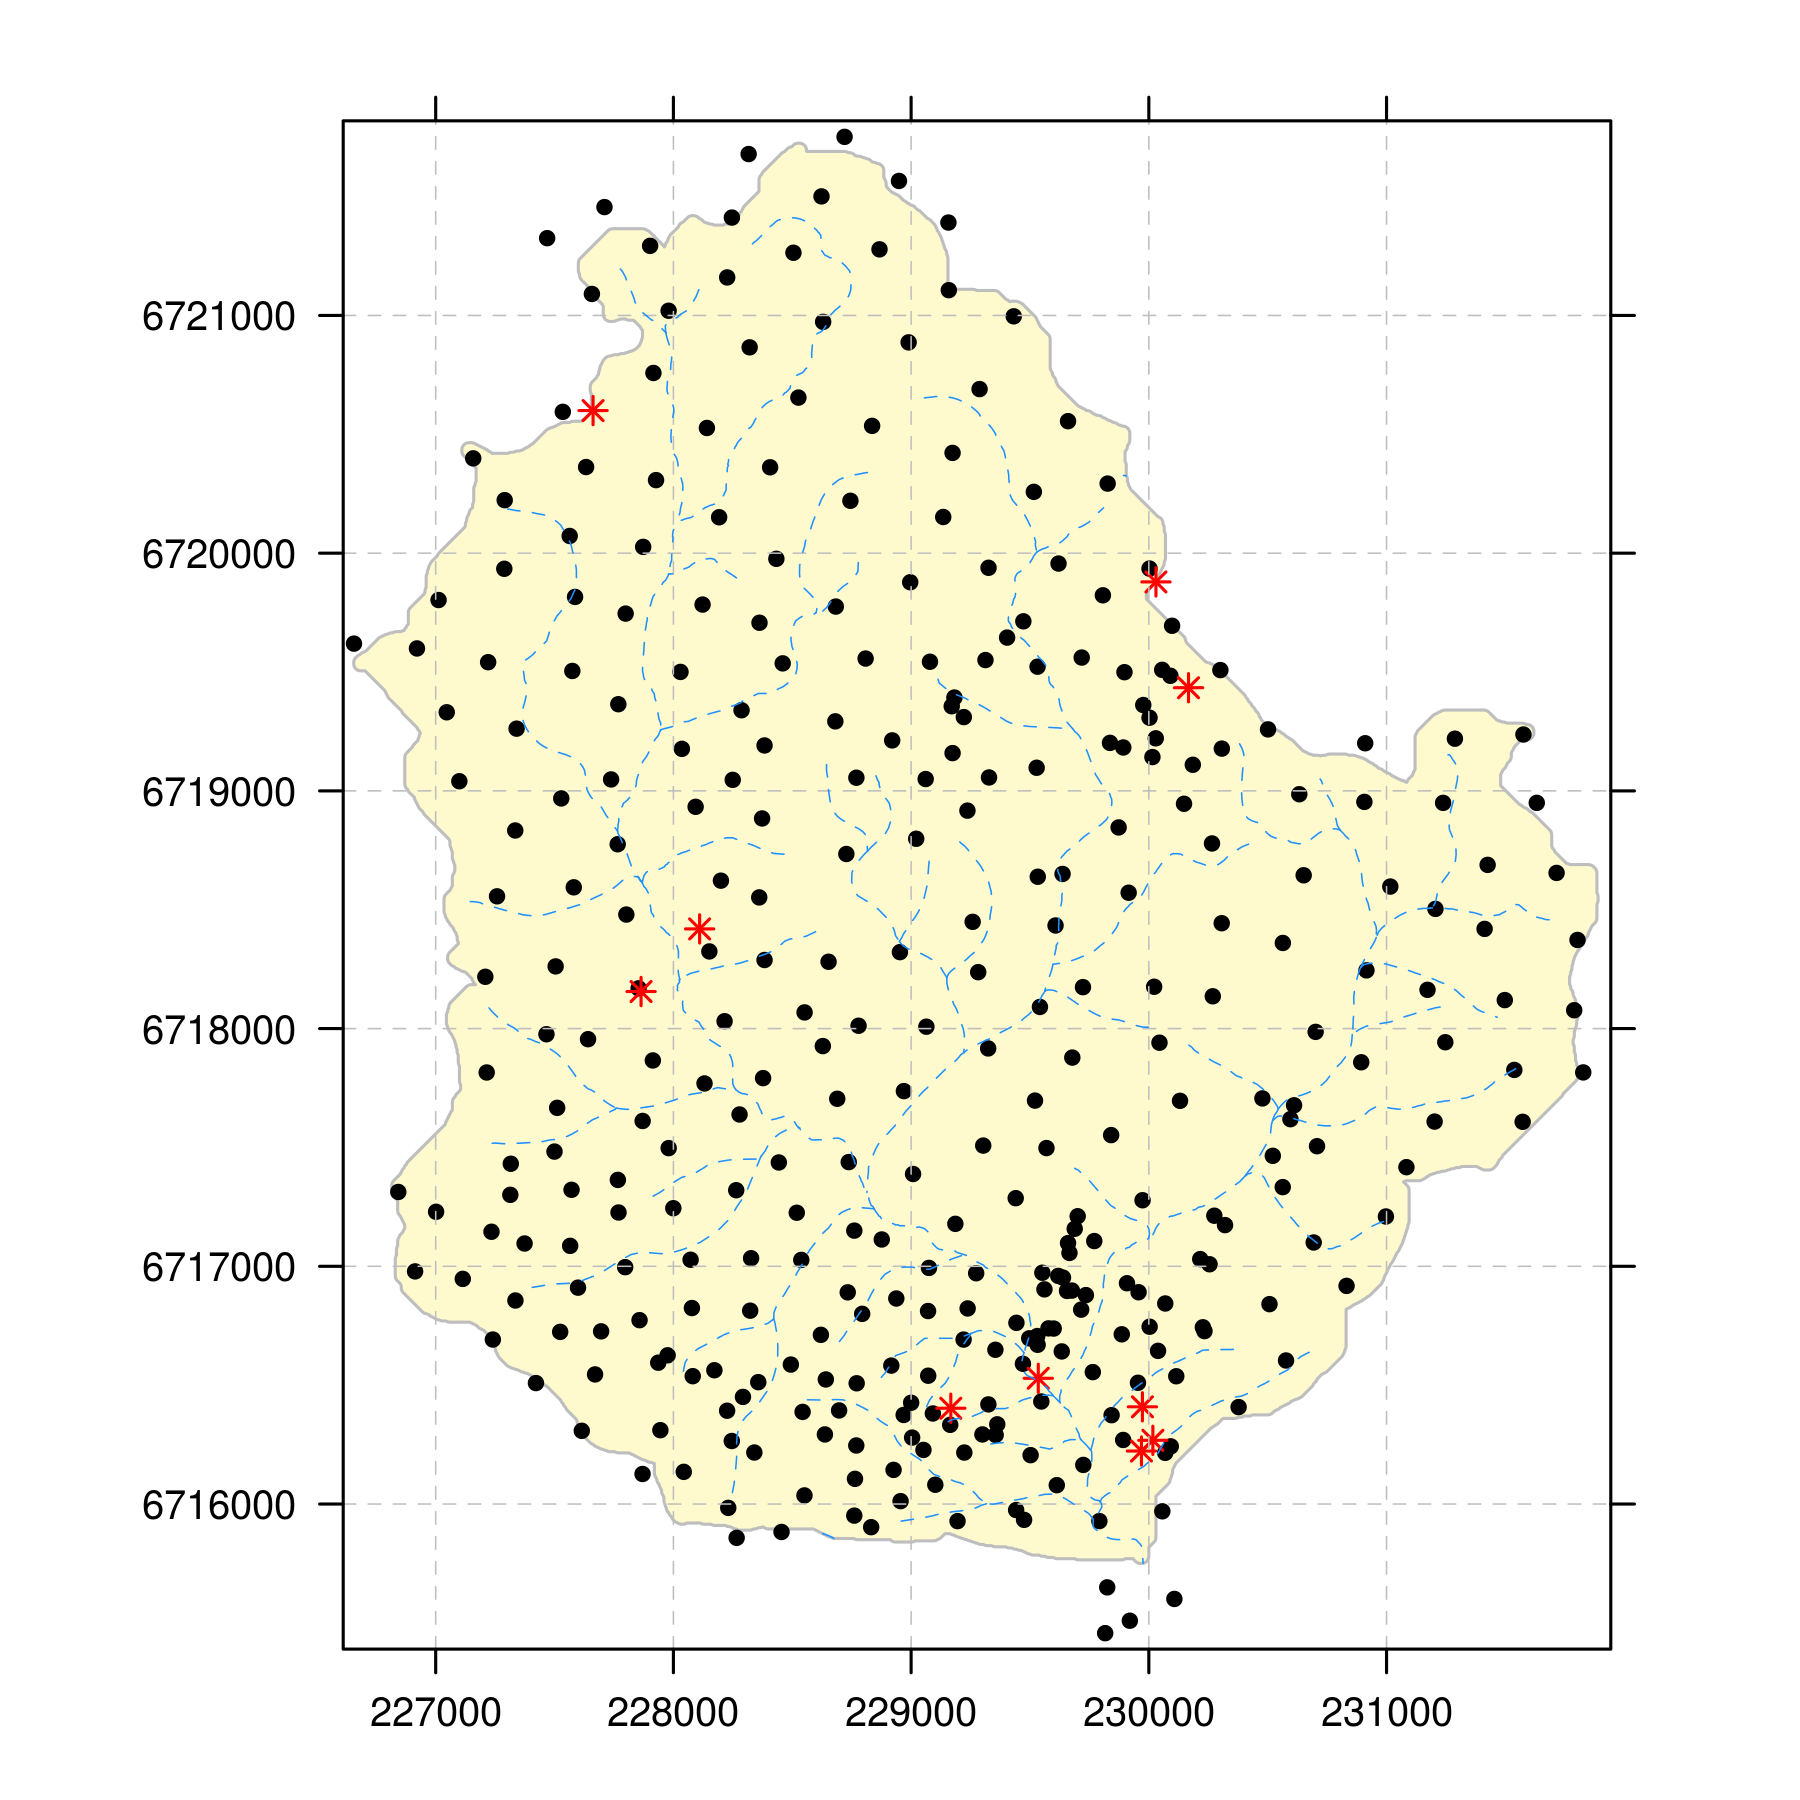
\includegraphics[width=0.90\textwidth]{fig/chap04-subsets-I-III}
\caption[Spatial distribution of \emph{Subset I} and \emph{Subset III}.]{Spatial distribution of the point 
soil observations contained in \emph{Subset I} ($n = 340$, black solid circles) and \emph{Subset III} ($n = 
10$, red stars) of the Santa Maria dataset. The drainage network is shown in the background (blue 
dashed line) to give an idea of how the locations of soil observations is related to terrain features.}
\label{fig:chap04-subsets-I-III}
\end{figure}

Georeferencing was done in the field using a Global Navigation Satellite System (GNSS) receiver with a 
horizontal positional error of less than \SI{\pm8}{\metre} positioned approximately at the centre of the
sampling area. Sometimes, the horizontal positional error was larger than \SI{\pm8}{\metre} due the effects
of vegetation, terrain, and satellite configuration. In these cases, observation locations 
were georeferenced in the office using \SI{1}{\metre} spatial resolution Google Earth\rr{} imagery 
with 
positional horizontal error of \SI{\pm6}{\metre} (\autoref{tab:chap05-google-geo-val}).

Every observation was identified with a number in increasing order, following the order in which the 
observations were made (\num{001}--\num{340}). A total of \num{17}~field campaigns were carried out, yielding 
an observation density of about \num{18}~observations per \si{\kilo\metre\squared}.

\subsection{Subset II}
\label{sec:chap04-subset-ii}

The second subset ($n = 60$, \autoref{fig:chap04-subset-II}) was produced in the years \num{2012} and 
\num{2013}, and was intended to constitute an independent dataset for validation purposes. Because of the many 
access limitations (geographic barriers and prohibition by landowners) and shortage of workforce, budget, 
infrastructure and time faced in previous field campaigns, researchers chose to employ transect (cluster) 
sampling \cite{MiguelEtAl2012, Moura-BuenoEtAl2012, Samuel-RosaEtAl2013}. They started defining the population 
of transects using their knowledge of the study area, taking into account the factors that they thought 
determined the spatial distribution of soil properties. Each researcher (three) delineated $m = 60$ easily 
accessible, straight transects of \SI{400}{\metre} following the spatial gradients of selected environmental 
features (topography, geology, vegetation, land use, and soils), totaling 180 transects. Accordingly, 
knowledge of existing roads, human settlements, water bodies, and other access limitations was used as well. 
The activity was carried out using \googlearth{} imagery of the years of \num{2008} and \num{2009}.

\begin{figure}[!ht]
\centering
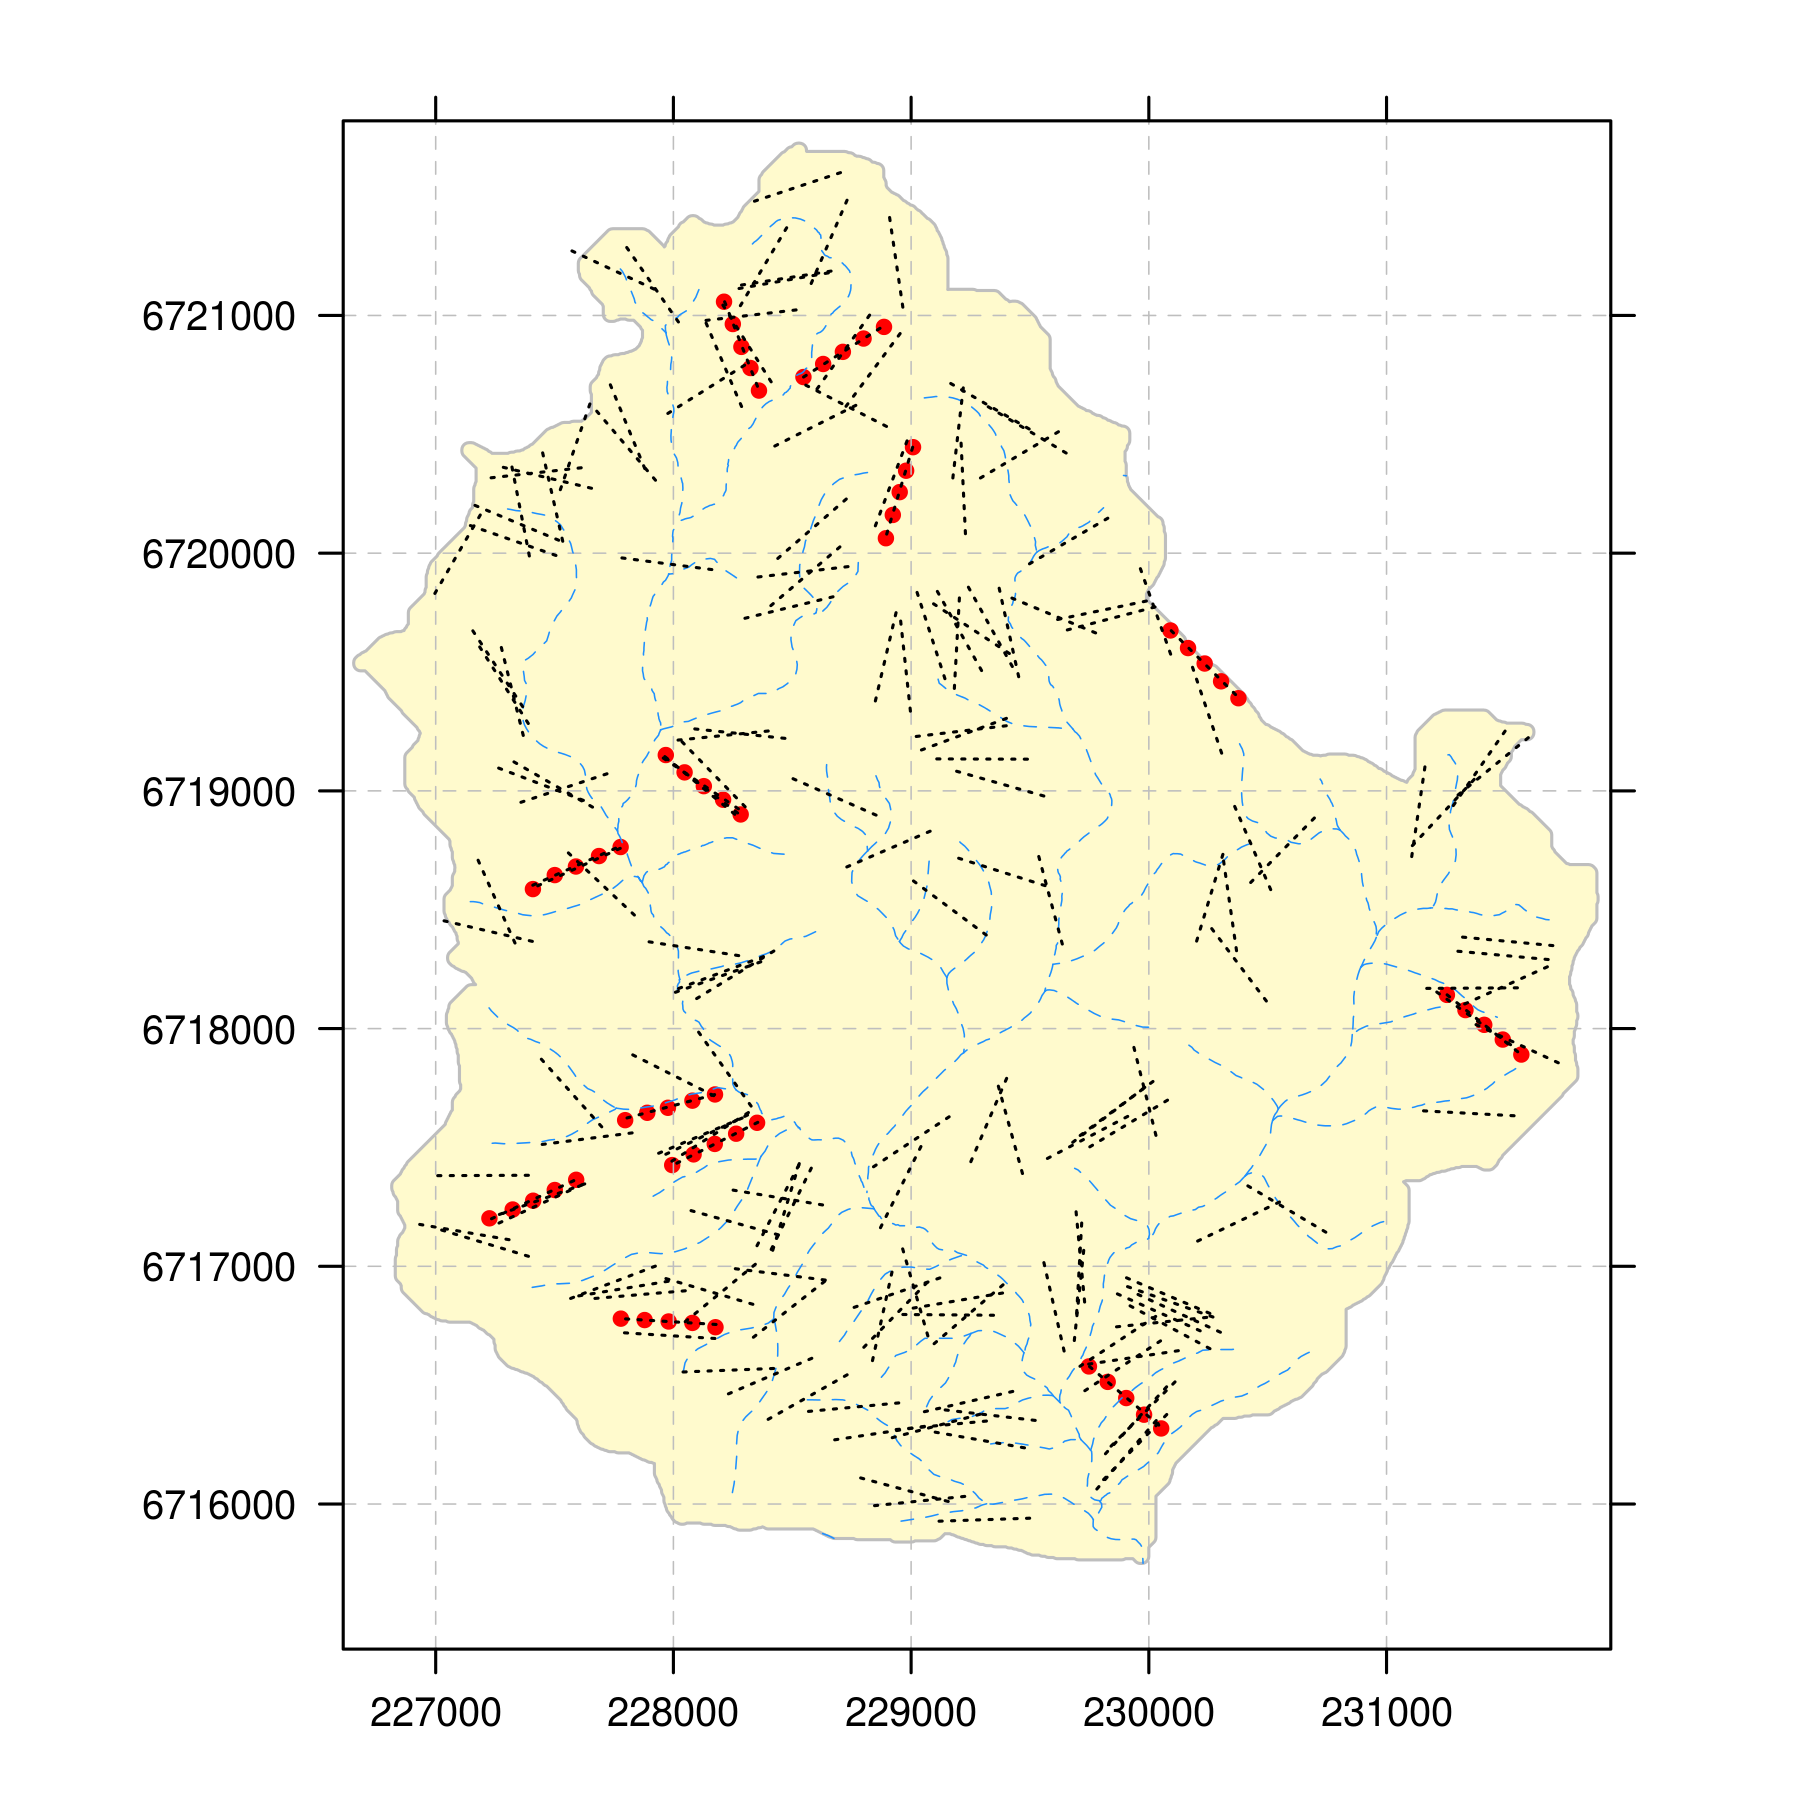
\includegraphics[width=0.90\textwidth]{fig/chap04-subset-II}
\caption[Twelve transects were selected using simple random sampling to yield $n = 60$ validation 
observations]{Three soil spatial modellers manually drew 180 straight transects (black dotted lines) aligned 
in the direction of maximum expected spatial variation of environmental conditions. They avoided locations 
where it was known that geographic barriers or landowners would impede the access to make soil observations. 
Twelve transects were probabilistically selected using simple random sampling to yield $n = 60$ validation 
observations (red solid circles) separated by equidistant intervals of \SI{100}{\metre}. The drainage network 
is shown in the background (blue dashed line) to give an idea of how the location and direction of transects 
is related to terrain features.}
\label{fig:chap04-subset-II}
\end{figure}

Twelve out of the $m = 180$ transects were randomly selected using as many iterations as necessary until 
there were no intersecting transects, and there was at least one transect in each of the three major 
geomorphological units of the study area (\textit{Planalto}, \textit{Rebordo do Planalto}, and 
\textit{Depressão Periférica}). Finally, $n = 5$ observation locations, separated by equidistant intervals of 
\SI{100}{\metre}, were selected in each transect. Observation locations were named with a number in increasing 
order, following the order in which the observations were made, starting from \num{341} (\num{341}--\num{400}).

Observation locations were identified in the field using a GNSS receiver with a horizontal positional error
of less than \SI{\pm8}{\metre}. A single soil pit was opened within a radius of \SI{2}{\metre} from the 
predefined observation location. Soil sampling and description was carried out using the same procedure used 
with \emph{Subset I}, except that in Subset II a single pit was observed. More accurate geographic coordinates 
were collected in the field using a Differential Global Positioning System (DGPS) with a horizontal positional 
error of less than \SI{1}{\centi\metre}.

\subsection{Subset III}

The third subset ($n = 10$) contains data compiled from the studies of \citeonline{Pedron2005} and
\citeonline{Miguel2010}, specifically from the uppermost A horizon of modal soil profiles whose locations 
were purposively selected using tacit knowledge after a preliminary area-class soil map had been produced 
and/or the observations included in \emph{Subset I} had been made. The researchers aimed at observation 
locations that they understood as being most representative of the soil mapping units depicted in their 
respective area-class soil maps. A single soil sample was taken from each of the described soil horizons and 
used for laboratory analysis (see below). The resulting depth of the uppermost A horizons varies from \num{12} 
to \SI{30}{\centi\metre}, with a mean of \SI{22.6}{\centi\metre}. Georeferencing was carried using a GNSS 
receiver with a horizontal positional error of less than \SI{\pm8}{\metre} positioned at the observation 
location. Data are identified in the Santa Maria dataset using the same identification that was used in the 
studies from where they were compiled.

\section{FIELD DESCRIPTION}

Several environmental features were described at the observation locations. The next sections present a 
description of how this was done.

\subsection{Land Use}

Land use (\texttt{LAND}) was assessed in the years of \num{2008} and \num{2009} using data collected in the 
field and Google Earth imagery. Five land uses were identified: native forest (primary or secondary), 
shrubland 
(abandoned areas with predominance of shrub-sized vegetation, known in Brazil as \emph{capoeira}), animal 
husbandry (grasslands), forestry (\textit{Eucalyptus spp.} and \textit{Pinus spp.}), and annual crop 
agriculture. Other 
land uses such as human settlements and water bodies were not observed/sampled.

\subsection{Geology}

Soil parent material (\texttt{PARENT}, sedimentary or igneous), geologic formation (\texttt{GEO}), and 
lithology (\texttt{LITHO}) was inferred from direct observation of soil properties and local environmental 
features in the field. Existing geologic maps were used only when soil characteristics and environmental 
features were insufficient to reach an agreement about the most likely soil parent material, geologic 
formation, and lithology.

\subsection{Soil Classification}

The most likely soil classification (\texttt{TAXON}) was inferred in the field using direct observation of 
soil 
properties (\SI{20}{\centi\metre}-deep soil pits and auger holes down to the diagnostic subsurface horizon or 
bedrock) and local environmental features. Soil taxon was inferred only to the second categorical level of 
the Brazilian System of Soil Classification \cite{SantosEtAl2013a} because further levels require data that 
were not observed in the field.

% TODO: move this description of the soil taxa to the metadata file.
% RF - Neossolo Flúvico, RL - Neossolo Litólico, RR - Neossolo Regolítico, RQ - Neossolo 
% Quartzarênico, PV - Argissolo Vermelho, PVA - Argissolo Vermelho-Amarelo, PA - Argissolo 
% Amarelo, PBAC - Argissolo Bruno-Acinzentado, SX - Planossolo Háplico, CX - Cambissolo Háplico.

\subsection{Slope}

The slope gradient (\texttt{SLOPE}, \si{\percent}) was measured using a clinometer, the observer and target 
being at a constant height above the ground. The distance between observer and target was between 
\SI{30}{\metre} (dense forests) and \SI{50}{\metre} (open fields).

\subsection{Drainage}

Soil drainage status (\texttt{DRAIN}) was inferred visually from soil features observed with an auger using 
the 
classification scheme proposed by \citeonline{SantosEtAl2013}.

\subsection{Coarse Fragments and Rock Outcrops}

Presence of coarse fragments (\texttt{FRAG}) -- soil material of diameter \SI{>2}{\milli\metre} -- was 
described as a binary variable, that is, a value of \num{1} (one) was annotated when coarse fragments were 
present, and \num{0} (zero) otherwise. The same approach was adopted to describe the presence of rock outcrops 
(\texttt{ROCK}). The quantity of coarse fragments (\texttt{GRAVEL}, \si{\percent}) was estimated visually in 
some observation points.

It is worth noting that the approach employed to describe the presence of coarse fragments and rock outcrops is 
not in line with the standard soil description guidelines currently used in Brazil. The reason for this is that 
these soil properties were understood as being secondary at the time of sampling. As such, it seemed reasonable 
to record only their presence/absence.

\subsection{Canopy}

% TODO: add three figures as examples of each class.
Soil coverage with vegetation (\texttt{CANOPY}) was inferred visually in the field using three classes: low 
(\SI{<25}{\percent}), medium (\SIrange{25}{75}{\percent}), and high (\SI{>75}{\percent}).

\subsection{Additional Information}

Additional information was recorded at each observation location during the field campaigns. They refer to 
peculiarities of each observation location and were not recorded in a systematic way.

\section{LABORATORY ANALYSIS}
\label{sec:chap04-laboratory}

Soil samples were air dried, crushed and passed through a \SI{2}{\milli\metre}-sieve prior to laboratory 
analyses using the methods described in the next sections. One or more laboratory replicates were used to 
calculate analytical errors.

\subsection{Soil Organic Fraction}
\label{sec:chap04-organic}

The soil organic carbon content (\texttt{ORCA}, \si{\gram\per\kilo\gram}) was determined using the method of
\citeonline{Mebius1960} modified by \citeonline{YeomansEtAl1988} as described by \citeonline{ClaessenEtAl1997}.

\def\footsulfochromic{\footnote{See a detailed description of the sulfochromic solution, or chromic acid, at 
\href{http://en.wikipedia.org/wiki/Chromic_acid}{Wikipedia}.}}

Sample aliquots of \num{0.050} to \SI{0.500}{\gram} were placed in glass digestion tubes 
(\SI{80}{\milli\liter}). The amount of sample used varied according to the ORCA estimated by visual 
interpretation of soil colour. Every digestion tube received an aliquot of \SI{10}{\milli\liter} of 
sulfochromic solution\footsulfochromic{} [\SI{0.067}{\mole\per\liter} potassium bichromate solution
(\ce{K2Cr2O7}) in the presence of concentrated sulphuric acid (\ce{H2SO4})] and a small reflux funnel 
to avoid loss of reagent during digestion. A digestion block with capacity for \num{40}~samples was used:
\num{36}~tubes with soil sample plus \num{3}~tubes with blank plus \num{1}~tube with \ce{H2SO4} and a
thermometer for temperature control. Digestion at \SI{150}{\celsius} last \SI{30}{\minute}. Three blanks 
were prepared and set aside at room temperature to estimate the loss of reagent due to heat in the digestion 
block. After digestion the tubes were set aside at room temperature to cool down. Next, the solution was 
transferred to Erlenmeyer flasks (\SI{250}{\milli\liter}) with \SI{60}{\milli\liter} of distilled water and
\SI{2}{\milli\liter} of concentrated orthophosphoric acid [\ce{H3PO4}] and \num{3}~drops of 
\SI{1}{\percent}~diphenylamine). The solution was titrated using \SI{0.1}{\mole\per\liter} ammonium ferrous
sulphate (\ce{FeSO4(NH4)2 * 6H2O}) until persistent green colour. The results were multiplied by \num{1.11}
to correct to the standard method (dry combustion).

The soil organic matter content of the observations compiled from \citeonline{Pedron2005} was determined 
using the method described by \citeonline{TedescoEtAl1995}. Sample aliquots of \SI{2.5}{\milli\liter}
were placed in Erlenmeyer flasks (\SI{50}{\milli\liter}). Every Erlenmeyer flask received an aliquot of 
\SI{15}{\milli\liter} of \SI{0.067}{\mole\per\liter} sulfochromic solution (\ce{Na2Cr2O7 + H2SO4}). The 
flasks were heated in a water bath at \num{75} to \SI{80}{\celsius} during \SI{30}{\minute} and shaken 
for \SI{5}{\minute}. A water aliquot of \SI{15}{\milli\liter} was added to the flask and let overnight 
(\num{15} to \SI{18}{\hour}). In the next day, an aliquot of \SI{3.0}{\milli\liter} was sampled to a 
small cup with \SI{3.0}{\milli\liter} of distilled water. The absorbency of the supernatant was measured 
at \SI{645}{\nano\metre}. The results were transformed to organic carbon content using the Van Bemmelen 
factor (\num{1.724}), the result assumed to be equivalent to soil organic carbon content measured using the 
standard method. The results are expressed using a volume-basis and were converted to a mass-basis using a
1:1 relation because the mass of the sample aliquot used in the analyses is unknown.

\subsection{Particle Size Analysis}
\label{chap:chap04-granulometry}

\def\footsuzuki{\footnote{As far as I know, a comprehensive description of this method has not been 
published so far, neither in Portuguese nor in English. You can visit the homepage of the Soil Physics 
Laboratory of the Universidate Federal de Santa Maria at \url{https://coral.ufsm.br/fisicadosolo/} to get more 
information about the method or contact their developers.}}

Particle size analysis was performed using the pipette method, with the sand fraction (\texttt{SAND}, 
\SIrange{0.053}{2}{\milli\metre}, \si{\gram\per\kilo\gram}) determined by wet sieving, and the silt fraction 
(\texttt{SILT}, \SIrange{0.002}{0.053}{\milli\metre}, \si{\gram\per\kilo\gram}) calculated by difference. 
The analytical procedure is an adaptation\footsuzuki{} of the method of the Soil Conservation Service of 
the United States Department of Agriculture \cite{UnitedStates1972} made by the Soil Physics Laboratory of the 
\textit{Universidade Federal de Santa Maria} \cite{SuzukiEtAl2004, SuzukiEtAl2004a}.

First, a sample aliquot of \SI{20}{\gram} was placed in a \SI{100}{\milli\liter} glass container (height: 
\SI{10.5}{\centi\metre}; diameter: \SI{2.75}{\centi\metre}; weight: \SI{85}{\gram}). Two nylon spheres with a 
diameter of \SI{1.71}{\centi\metre} and weighting \SI{3.04}{\gram} (density: \SI{1.11}{\g\per\cm\cubic}) were 
added to act as physical disaggregating agents. Then, an aliquot of \SI{10}{\milli\liter} of 
\SI{1}{\mole\per\liter} sodium hydroxide (\ce{NaOH}) solution was added to act as chemical dispersing agent 
along with \SI{40}{\milli\liter} of distilled water. The glass container was closed with a plastic cap, 
manually shaken for \SI{10}{\second}, and placed in a horizontal mechanical shaker with capacity for 
\num{85}~samples. The suspension was left to stand overnight (\SI{10}{\hour}). In the next day the suspension 
was submitted to horizontal mechanical agitation during \SI{4}{\hour} at \si{120} cycles per minute 
\cite{SuzukiEtAl2004, SuzukiEtAl2004a}.

After horizontal agitation, the suspension was poured in a plastic graduated cylinder with capacity for 
\SI{1000}{\milli\liter} using a glass funnel and a metal sieve to hold the two nylon spheres. The suspension 
in 
the graduated cylinder was completed to \SI{1000}{\milli\liter} and homogenized using a hand stirrer 
(\SI{30}{\second}). The suspension was allowed to stand until sedimentation was complete. The time needed was 
calculated using the Stokes’ law with the temperature measured in a graduated cylinder filled with distilled 
water.

%TODO provide a more detailed description of how CLAY was determined as well as of the oxidative
%treatment with H2O2.

The clay fraction (\texttt{CLAY}, \SI{<0.002}{\milli\metre}, \si{\gram\per\kilo\gram}) was determined by the 
pipette method. Soil samples with organic matter content \SI{>5}{\percent} were submitted to oxidative 
treatment with hydrogen peroxide (\ce{H2O2}) prior to the analysis following the recommendations of
\citeonline{ClaessenEtAl1997}.

%The sand fraction was separated into five size classes:
%
%\begin{itemize}
%\item \SIrange{1.00}{2.00}{\milli\metre}: very coarse sand;
%\item \SIrange{0.50}{1.00}{\milli\metre}: coarse sand;
%\item \SIrange{0.25}{0.50}{\milli\metre}: median sand;
%\item \SIrange{0.106}{0.25}{\milli\metre}:fine sand;
%\item \SIrange{0.053}{0.106}{\milli\metre}: very fine sand.
%\end{itemize}

% The clay fraction (\textless0.002~mm) was initially determined by the pipette method without any 
% pretreatment. A 1~mol~L$^{-1}$ NaOH solution was used as the dispersing agent, with the addition of two 
% nylon spheres as disaggregating agent plus horizontal mechanical agitation during 4~hours 
% \cite{SuzukiEtAl2004}.

% A propor{\c{c}}{\~{a}}o da fra{\c{c}}{\~{a}}o argila dispersa em {\'{a}}gua foi determinada conforme 
% descrito acima para a fra{\c{c}}{\~{a}}o argila total. A diferen{\c{c}}a {\'{e}} que n{\~{a}}o foi usado o 
% agente dispersante (NaOH) e o agente desagregante (esferas de nylon) \cite{ClaessenEtAl1997}.

\subsection{Soil Density}
\label{chap:chap04-bude}

% TODO: Provide a more detailed description of how this is done.
The bulk soil density (\texttt{BUDE}, \si{\mega\gram\per\cubic\metre}) was determined using the core method 
with a metallic ring (height: \SI{3}{\centi\metre}; diameter: \SI{5}{\centi\metre}) as described by 
\citeonline{ClaessenEtAl1997}. The bulk soil density was not determined in the locations where the soil was 
very shallow or stony.

\subsection{Exchangeable Bases and Acidity}
\label{chap:chap04-ecec}

The exchangeable calcium (\texttt{CALC}, \si{\milli\mole\per\kilo\gram}) and magnesium (\texttt{MAGN}, 
\si{\milli\mole\per\kilo\gram}) were determined by atomic absorption spectroscopy after extraction with 
\SI{1.0}{\mole\per\liter} \ce{KCl} solution using the method described by \citeonline{ClaessenEtAl1997}. 
The exchangeable sodium (\texttt{SODI}, \si{\milli\mole\per\kilo\gram}) and potassium (\texttt{POTA}, 
\si{\milli\mole\per\kilo\gram}) were extracted with a \SI{0.05}{\mole\per\liter} \ce{HCl} solution plus 
\SI{0.025}{\mole\per\liter} \ce{H2SO} (Mehlich-\num{1} solution). Both were quantified by means of flame 
atomic emission spectrometry using the method described by \citeonline{TedescoEtAl1995}.

The exchangeable acidity (\texttt{EXAC}, \si{\milli\mole\per\kilo\gram}) was extracted using the same 
\SI{1.0}{\mole\per\liter} \ce{KCl} solution used to extract the exchangeable calcium and magnesium. It was 
determined by titrimetry with \SI{0.025}{\mole\per\liter} \ce{NaOH} solution as described by 
\citeonline[p.~103]{ClaessenEtAl1997}.

% TODO: Include POAC in the database and improve the description of how it was determined.
% The potential acidity (POAC, \si{\milli\mole\per\kilo\gram}) was determined with \SI{1.0}{\mole\per\liter} 
% calcium acetate solution at pH~\num{7.0} and titrated with \SI{0.0606}{\mole\per\liter} \ce{NaOH} solution 
% as described by \citeonline{ClaessenEtAl1997}.

The effective cation exchange capacity (ECEC, \si{\milli\mole\per\kilo\gram}) was defined as the sum of 
exchangeable bases and exchangeable acidity, i.e. 

\begin{equation*}
 \texttt{ECEC} = \texttt{CALC} + \texttt{MAGN} + \texttt{POTA} + \texttt{SODI} + \texttt{EXAC}.
\end{equation*}


% TODO: Provide a more detailed description of how these are calculated and include the data in the database.
% The sum of exchangeable bases (BASES) is given by the sum of the exchangeable calcium, magnesium, sodium and 
% potassium. The effective cation exchange capacity (ECEC) is given by the exchangeable acidity plus the 
% sum of exchangeable bases. The potential cation exchange capacity (CEC) is given by the potential acidity 
% plus the sum of exchangeable bases. Note that the standard method for determining exchangeable bases relies 
% on the use of barium chloride [BaCl$_2$]. The base saturation (BASA) is given by the sum of exchangeable 
% bases divided by the potential cation exchange capacity. The saturation of the ECEC with exchangeable 
% acidity, or the aluminum saturation (ALSA), is given by the sum of exchangeable bases divided by the 
% effective cation exchange capacity. The results are multiplied by 100. 

% \begin{figure}[!ht]
% \centering
% <<echo = FALSE>>=
% options(useFancyQuotes = FALSE)
% tmp <- read.table(
%  '~/projects/dnos-sm-rs/dnos-sm-rs-general/data/labData.csv', sep = ";",
%  header = TRUE, na.strings = 'na')
% lattice::trellis.par.set(
%  fontsize = list(text = 16, points = 15), axis.line = list(lwd = 0.01),
%  layout.widths = list(left.padding = 0, right.padding = 0),
%  layout.heights = list(top.padding = 0, bottom.padding = 0))
% aa <- pedometrics::plotHD(tmp$CLAY, xlab = 'CLAY')
% bb <- pedometrics::plotHD(tmp$ORCA, xlab = 'ORCA')
% cc <- pedometrics::plotHD(tmp$ECEC, xlab = 'ECEC')
% dd <- pedometrics::plotHD(na.exclude(tmp$BUDE), xlab = "BUDE")
% @
% \begin{minipage}[b]{63mm}
% \subcaption{}
% \centering
% <<intro-clay, fig = TRUE, echo = FALSE>>=
% print(aa)
% @
% \end{minipage}
% \begin{minipage}[b]{63mm}
% \subcaption{}
% \centering
% <<intro-orca, fig = TRUE, echo = FALSE>>=
% print(bb)
% @
% \end{minipage}
% \begin{minipage}[b]{63mm}
% \subcaption{}
% \centering
% <<intro-ecec, fig = TRUE, echo = FALSE>>=
% print(cc)
% @
% \end{minipage}
% \begin{minipage}[b]{63mm}
% \subcaption{}
% \centering
% <<intro-bude, fig = TRUE, echo = FALSE>>=
% print(dd)
% @
% \end{minipage}
% \caption{The four soil properties explored in this thesis: (a) clay content, (b) organic carbon
% content, (c) effective cation exchange capacity, and (d) bulk density. Each panel shows the sample
% histogram and summary statistics of the soil properties in their original scale ($\lambda = 1$), as
% well as the theoretical probability density function so that we can assess how good is the fit of
% the normal distribution to the data -- a product of the \Rpackage{pedometrics}.}
% \label{fig:intro-soil-properties}
% \end{figure}

\section{CONCLUSIONS}

The main goal of documenting the soil data contained in the Santa Maria dataset was to provide the reader the 
basis to understand the soil data used in the thesis, and also to support future soil spatial modelling 
exercises in 
the catchment of the DNOS reservoir.

As a result of an ongoing collaborative effort, this documentation will be improved in the near future as new 
studies are developed. We plan to include new figures to exemplify how field soil sampling was carried out. 
Details of non-standard soil description and analysis methods will likely be extended. This includes the 
oxidative 
treatment with \ce{H2O2} to which soil samples were submitted prior to particle size distribution analysis. 
For 
cases such as the ECEC, determined using a non-standard method, we plan to develop a study to calibrate a 
model 
to convert our results to the standard method for determining exchangeable bases, which uses barium chloride 
(\ce{BaCl2}) for saturation.

Other already existing soil data will also be included in the Santa Maria dataset and documented as well. 
These 
data have not been used in any study so far, including the potential acidity, sum of exchangeable bases, 
potential 
cation exchange capacity, base saturation, aluminium saturation, and the five size classes of the sand 
fraction.

Once a comprehensive documentation of the existing soil data has been constructed, we will prepare a basic 
spatial exploratory soil data analysis. We hope that our effort to properly document the soil data that we 
produced,
and make it freely available for use, will serve as an example for future soil spatial modelling studies 
developed 
elsewhere.

 % 4. The Santa Maria dataset -- soil data
% \artigotrue
\chapter{THE SANTA MARIA DATASET. PART II -- COVARIATE DATA}
\label{chap:chap05}
%\SweaveUTF8



%\def\ptkeys{}
%
%\begin{chapterabstract}{brazilian}{\ptkeys}
% Este é o resumo em português.
%\end{chapterabstract}

\def\enkeys{Area-class soil maps. Digital elevation models. Geological maps. Land use maps. Satellite images}
  
\begin{chapterabstract}{english}{\enkeys}
The Santa Maria dataset comprises a list of more than 100 covariates covering the catchment of the DNOS-CORSAN 
(\textit{Departamento Nacional de Obras de Saneamento}-\textit{Companhia Riograndense de Saneamento}) 
reservoir, 
located in the southern Brazilian state of Rio Grande do Sul. These covariates were derived from five freely 
available sources in two levels of spatial detail: area-class soil maps, digital elevation models, geological 
maps, land use maps, 
and satellite images. These covariate data are the outcome of projects that aimed at modelling various 
environmental 
features and were carried out as part of local (soil, geology, land use), regional (terrain, land use), and 
global (terrain, 
land use) mapping initiatives.
\end{chapterabstract}

\formatchapter

\section{INTRODUCTION}
\label{sec:chap05-intro}

\titlenote{This chapter is based on the studies \textit{Identifying and correcting oblique striping in the 
Topodata digital elevation model}, presented at the XXXIV Brazilian Congress of Soil Science 
\cite{Samuel-RosaEtAl2013c}, and \textit{Evaluation of freely available ancillary data used for detailed soil 
mapping in Brazil}, presented at the EGU General Assembly 2014 \cite{Samuel-RosaEtAl2014}. Also collaborated 
in the preparation of this document: Pablo Miguel (UFPel), Jean Michel Moura Bueno (UFSM), Ricardo Simão Diniz 
Dalmolin (UFSM), Lúcia Helena Cunha dos Anjos (UFRRJ), Gustavo de Mattos Vasques (Embrapa Soils), and Gerard 
B. 
M. Heuvelink (ISRIC -- World Soil Information).}

The Santa Maria dataset is a data set comprising spatially exhaustive covariate data produced in the 1980s, 
1990s, and 2000s covering the catchment of the DNOS-CORSAN reservoir, located in the southern border of the 
plateau of the Paraná Sedimentary Basin, in the city of Santa Maria, state of Rio Grande do Sul, Brazil. Some 
of these covariate data cover only part of the catchment, mainly the northern sector, which has an area of 
about
\SI{2000}{\hectare}, corresponding to about \SI{60}{\percent} of the entire catchment. These covariate data 
are the outcome of projects that aimed at modelling various environmental features and were carried out as 
part of local (soil, geology, land use), regional (terrain, land use), and global (terrain, land use) mapping 
initiatives.

Covariate data were harmonized to a reference grid of \SI{5}{\m} grid size. The coordinate reference 
system (CRS) is WGS1984 / UTM zone 22S, coded \href{http://spatialreference.org/ref/epsg/32722/}{\num{32722}} 
by the European Petroleum Survey Group (\href{http://www.epsg.org/}{EPSG}).

This document presents a description of the covariate data contained in the Santa Maria dataset, including the 
procedures for their production, as well as the processing methods employed. The original sources of the 
covariate data are freely available at the producers databases or in public libraries.

\section{GROUND CONTROL POINTS}
\label{sec:chap05-gcp}

All covariates were validated prior to their use. Horizontal (positional) validation was performed using a set 
of $n = 14$ validation points, here called ground control points (GCP), spread throughout and beyond the 
limits of the study area (\autoref{fig:chap05-field-gcps}). The location of the GCPs was defined based on 
the existence of easily identifiable geographical markers across the covariates, including road intersection, 
fence corners, and property entrances.

\begin{figure}[!ht]
\centering
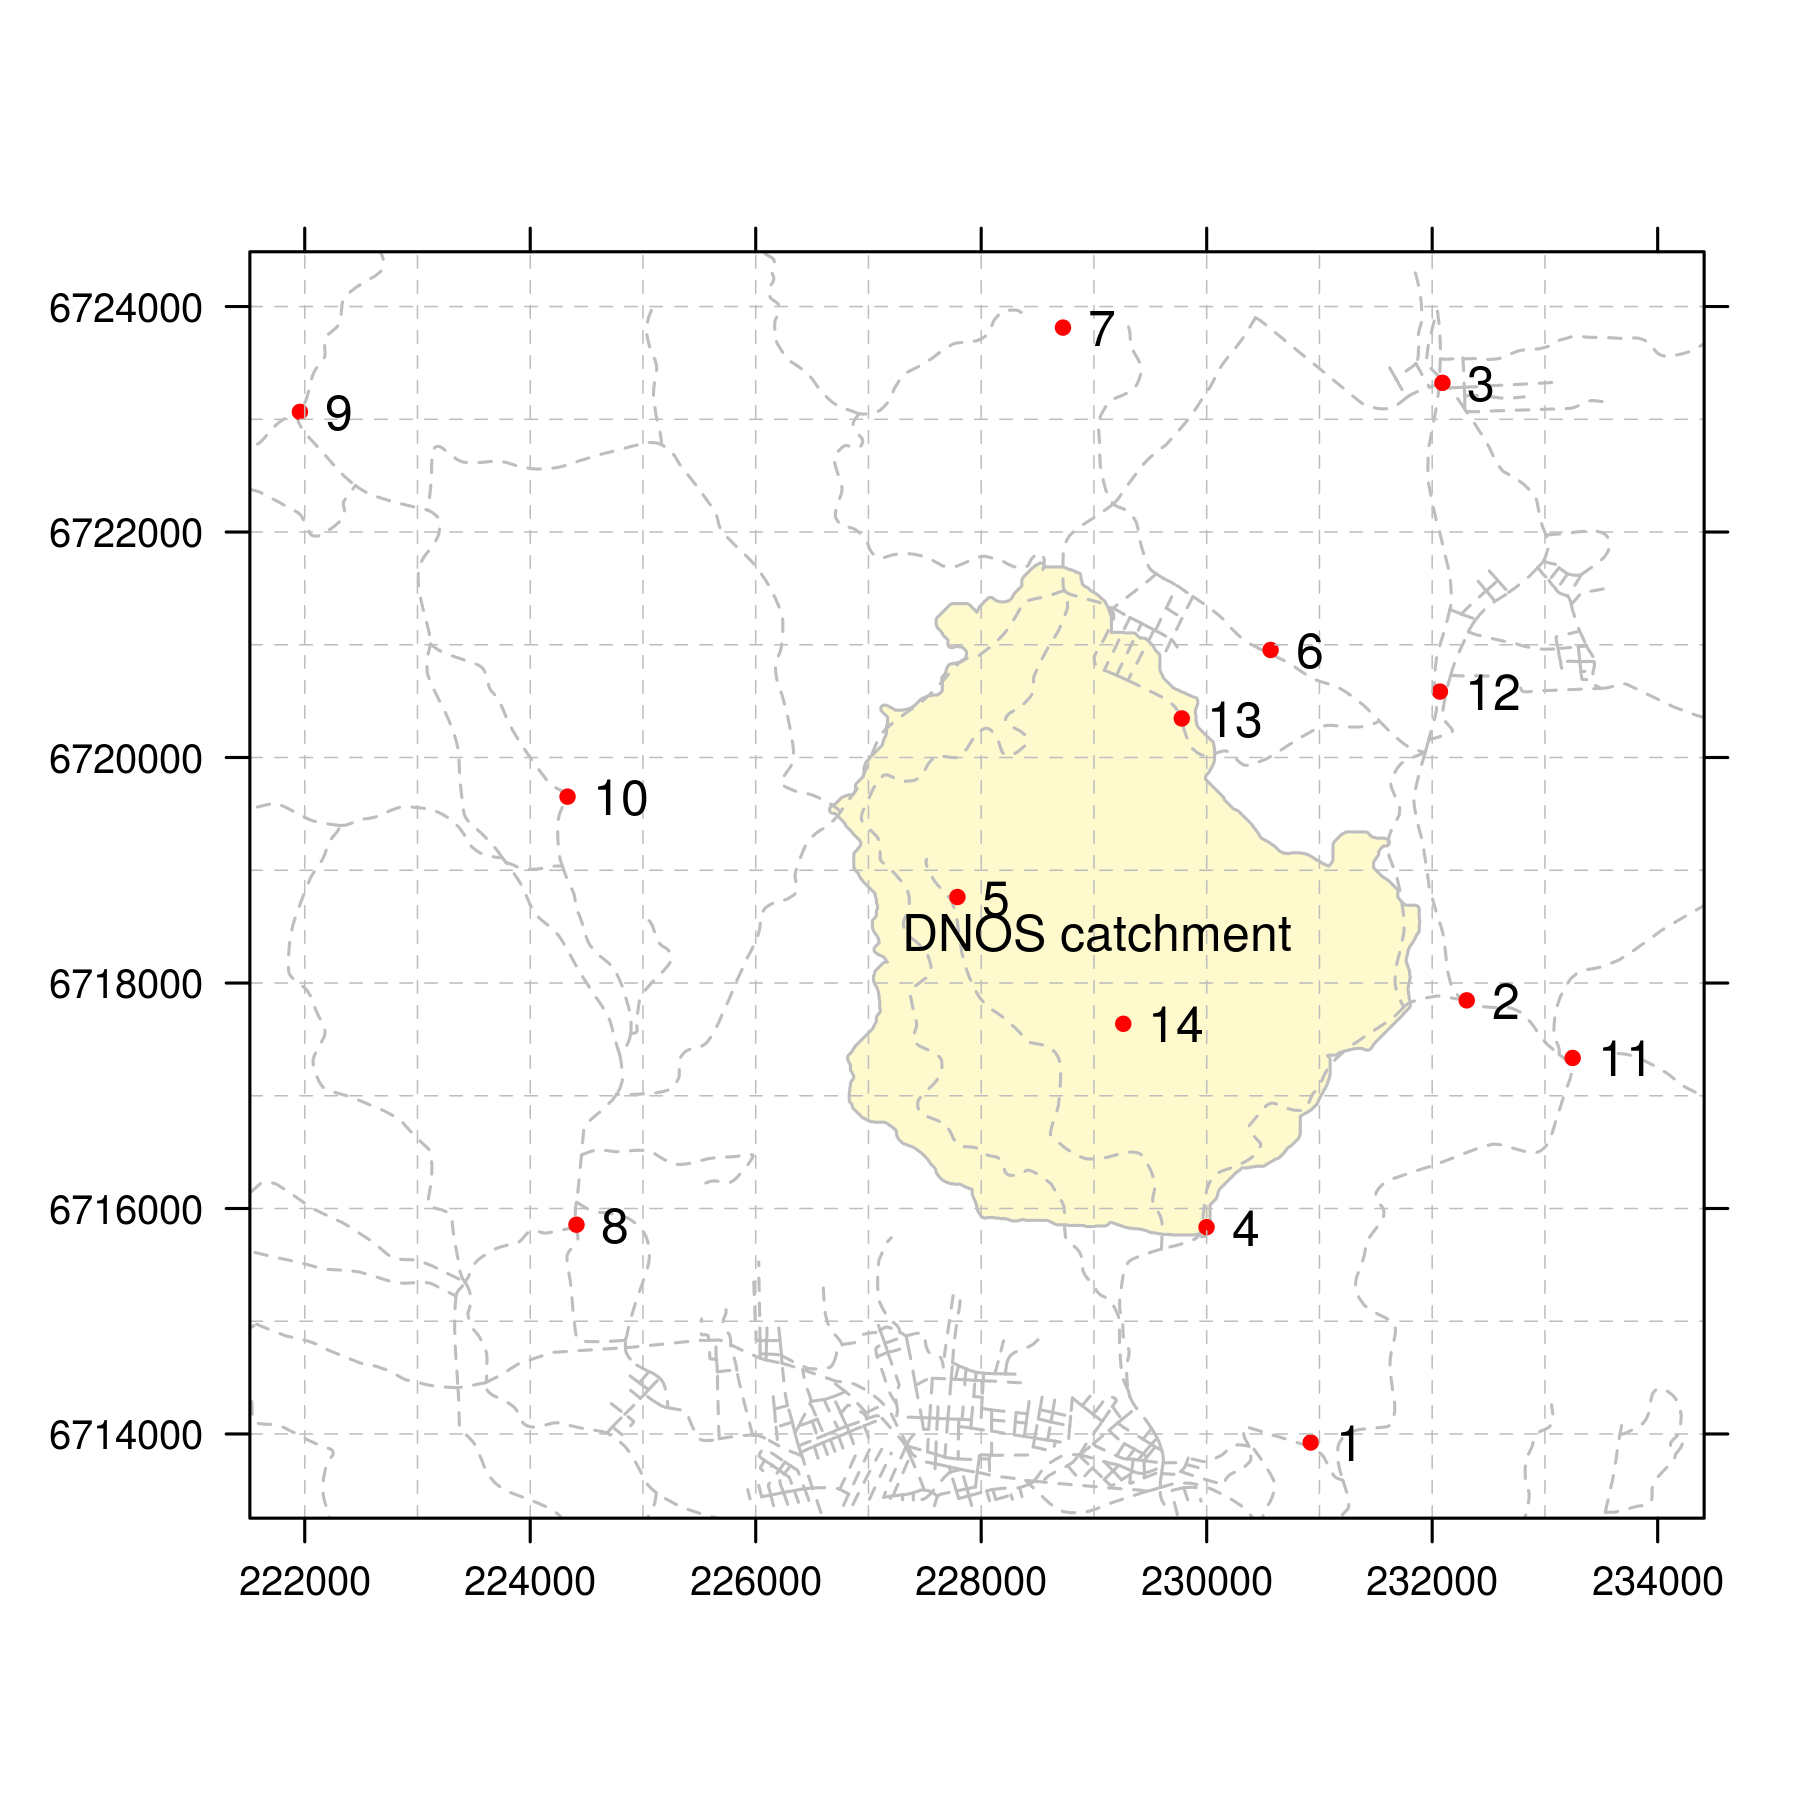
\includegraphics[width = 0.90\textwidth]{fig/chap05-field-gcps}
\caption[Ground control points used for the positional validation of the covariates.]{Spatial distribution of 
the ground control points ($n = 14$, red dots) used for the horizontal positional validation of covariates 
included in the Santa Maria dataset.}
\label{fig:chap05-field-gcps}
\end{figure}

Positional validation was performed comparing the x- and y-coordinates of GCPs (observed value) with the 
coordinates of the respective geographical markers visually identified on the covariates (predicted value). 
The differences in the observed and predicted x- and y-coordinates were used to calculate the mean error (ME, 
\si{\m}), mean absolute error (MAE, \si{\m}), and mean squared error (MSE, \si{\m\square}) to evaluate if 
there were differences in the accuracy and precision between coordinates. The error vector (or module, the 
euclidean distance between two points) and its azimuth (the orientation of the error vector) were computed as 
well for every point. The mean of the error vector and its azimuth give the size and orientation of the 
systematic error present in the covariates, while the square root of the mean squared error vector (RMSE) is a 
measure of the uncertainty about the true position of the covariate in the geographic space.

The field location of the GCPs is as follows (in Portuguese):

\begin{description}
 \item [GCP 01] Em Santa Maria, no lado direito da barragem de concreto do reservatório do DNOS-CORSAN, 
 \SI{6}{\m} antes de chegar a ponte sobre o vertedouro, a \SI{3}{\m} de distância do centro da estrada que 
 desce da rodovia federal BR158.
 
 \item [GCP 02] Na entrada da Estrada do Perau, Rua Gralha Azul, em Itaara, no centro do canteiro, entre o 
 outdoor e a árvore (\textit{Cedrella fissilis}), junto à rodovia federal BR158.
 
 \item [GCP 03] Na entrada de Itaara, próximo ao equipamento estático de fiscalização eletrônica de 
 velocidade, na rodovia federal BR158, a \SI{520}{\m} do Museu de Ufologia, em frente à Fruteira da 
 Esquina. Do outro lado da rodovia há uma torre, possivelmente de telefonia celular, e entrada para a mina de 
 extração de brita DallaPasqua, localizada a \SI{4}{\km} do local.
 
 \item [GCP 04] Em Santa Maria, na entrada da estrada de acesso ao cemitério do Bairro Campestre do Menino 
 Deus, do lado direito da Estrada do Perau (subindo), alinhado (\SI{50}{\cm}) com a frente das casas, a
 \SI{2,2}{\m} do muro, a \SI{6,5}{\m} do meio-fio da Estrada do Perau, a \SI{50}{\m} da ponte sobre o Rio
 Vacacaí-Mirim.
 
 \item [GCP 05] Na entrada do Rancho do Amaral, junto à porteira, no lado direito, fora da estrada, distante 
 \SI{1}{\m} de uma palmeira e \SI{1}{\m} do muro de pedras.
 
 \item [GCP 06] Em Itaara, na Avenida Etelvina, na beira da estrada, a \SI{2,5}{\m} do centro da estrada,
 alinhado (\SI{20}{\cm}) com a cerca que separa a floresta nativa do pomar de \textit{Citrus}~sp.~localizado 
 do outro lado da estrada.
 
 \item [GCP 07] Em Itaara, no lado esquerdo da entrada da estrada que dá acesso à mina de extração de brita
 DallaPasqua, sob a rede de transmissão de eletricidade. Localidade de Estação Pinhal. 
 
 \item [GCP 08] No Distrito de Santo Antão, na entrada da estrada para a Central de Tratamento de Resíduos
 da Caturrita, em frente à Escola Municipal de Ensino Fundamental Intendente Manoel Ribas.
 
 \item [GCP 09] Em São Martinho da Serra, na localidade de Água Negra, na bifurcação da estrada que vem de
 Santa Maria e que dá acesso à localidade de Campinas, junto à parada de ônibus, no canteiro no meio da
 bifurcação, \SI{40}{\m} distante do Piquete Laçador Jorge R.~da Silva, em frente ao Mercado do Ronaldo.
 
 \item [GCP 10] Na estrada de Santa Maria para São Martinho da Serra, em uma curva, no lado externo, próximo a
 duas pequenas árvores, alinhado (\SI{1}{\m}) com a cerca que marca a divisa entre duas propriedades e campo
 nativo. Em frente à propriedade com duas casas, uma delas com dois andares e quatro pequenos lagos nos
 fundos. Depois da capela Santo Antão.
 
 \item [GCP 11] Em Itaara, na entrada da estrada que dá acesso à Brita Pinhal, junto à rodovia federal BR185,
 ao lado (distante \SI{5}{\m}) do corte no terreno expondo a rocha de arenito da Formação Botucatu,
 \SI{15}{\m} distante do poste da linha de transmissão de eletricidade da companhia AES, na entrada para a
 localidade de Rincão dos Minello.
 
 \item [GCP 12] Em Itaara, em frente ao lago da SOCEPE, na entrada da cidade, junto à rodovia federal BR158,
 próximo ao Bar e Armazém Ricardo, deslocado em \SI{1}{\m} para dentro do passeio em relação ao alinhamento 
 dos postes da rede elétrica.
 
 \item [GCP 13] Em Itaara, na Vila Etelvina, alinhado com a cerca (a \SI{30}{\cm}) que divide duas 
propriedades, uma à 
 esquerda coberta com floresta nativa/exótica e outra à direita ocupada com lavoura de culturas anuais. O ponto 
está 
 locado no lado oposto. Plantação de videiras logo acima, no divisor de águas.
 
 \item [GCP 14] Em Itaara, na estrada que sobe para a propriedade do Sr. Antoninho Luccas, logo após o término 
 da subida íngreme com calçamento apenas nos trilhos, no final da floresta e início do campo nativo, alinhado 
 (a \SI{20}{\cm}) com a cerca dos dois lados da estrada. Locado \SI{1}{\m} distante do moirão da cerca do 
 lado esquerdo subindo, no interior da estrada.
\end{description}

Attribute validation of soil, geologic, and land use maps, and digital elevation models was done using a set of 
$n = 60$ 
validation points located along $m = 12$ linear transects. The procedures for obtaining soil, geologic, land 
use, and elevation data at these validation points is described in \autoref{chap:chap04}, 
\autoref{sec:chap04-subset-ii}. Such a validation exercise was carried out because these maps originally had no 
accompanying validation information.

% TODO: figure with GCPs used to orthorectify satellite images. Show the bounding box of the image and the 
% boundary 
% of the study area.
% \begin{figure}
%  \centering
%  \includegraphics[width=\textwidth]{fig/ortho-gcps}
%  \caption{Ground control points used to orthorectify the image produced by Landsat-5 Thematic 
% Mapper.}
%  \label{fig:chap05-ortho-gcps}
% \end{figure}

\section{AREA-CLASS SOIL MAPS}
\label{sec:chap05-soil-maps}

Two area-class soil maps are included in the Santa Maria dataset. The first of them (\soilOld{}) was published 
at a \scale{100000} \cite{AzolinEtAl1988}. Existing area-class soil maps and technical reports 
\cite{Brasil1973, Azolin1977, MacielEtAl1987a, MacielEtAl1987, AbraoEtAl1988}, and sparse field observations 
were used to elaborate the preliminary legend of the soil map. Aerial photographs (\scale{60000}) were used to 
produce the first draft of the soil map. Field checks of soil polygons (i.e. mapping units) was done along the 
road network (i.e. by convenience sampling). These observations were used to estimate the composition 
(occurrence and spatial distribution of soil taxa) of soil mapping units. They were also used to review the 
first draft of the soil 
map. The final version of \soilOld{} was prepared using topographic maps originally published at a 
\scale{50000} and resampled to a \scale{100000}. Soil classification followed the criteria adopted by the 
Brazilian soil science community at that time \cite{Brasil1973, CamargoEtAl1982, Carvalho1982, LemosEtAl1982, 
OlmosEtAl1982}. Identification of soil taxa was performed based on morphological features, analytical data 
compiled from existing technical reports, and analysis of soil samples collected from soil profiles observed 
along the road network. Description of each soil mapping unit includes the estimated area (\si{\hectare}) and 
the approximate taxonomic composition (\si{\percent}).

\begin{figure}[!ht]
\centering
\begin{minipage}[b]{0.45\textwidth}
\subcaption{}
\centering
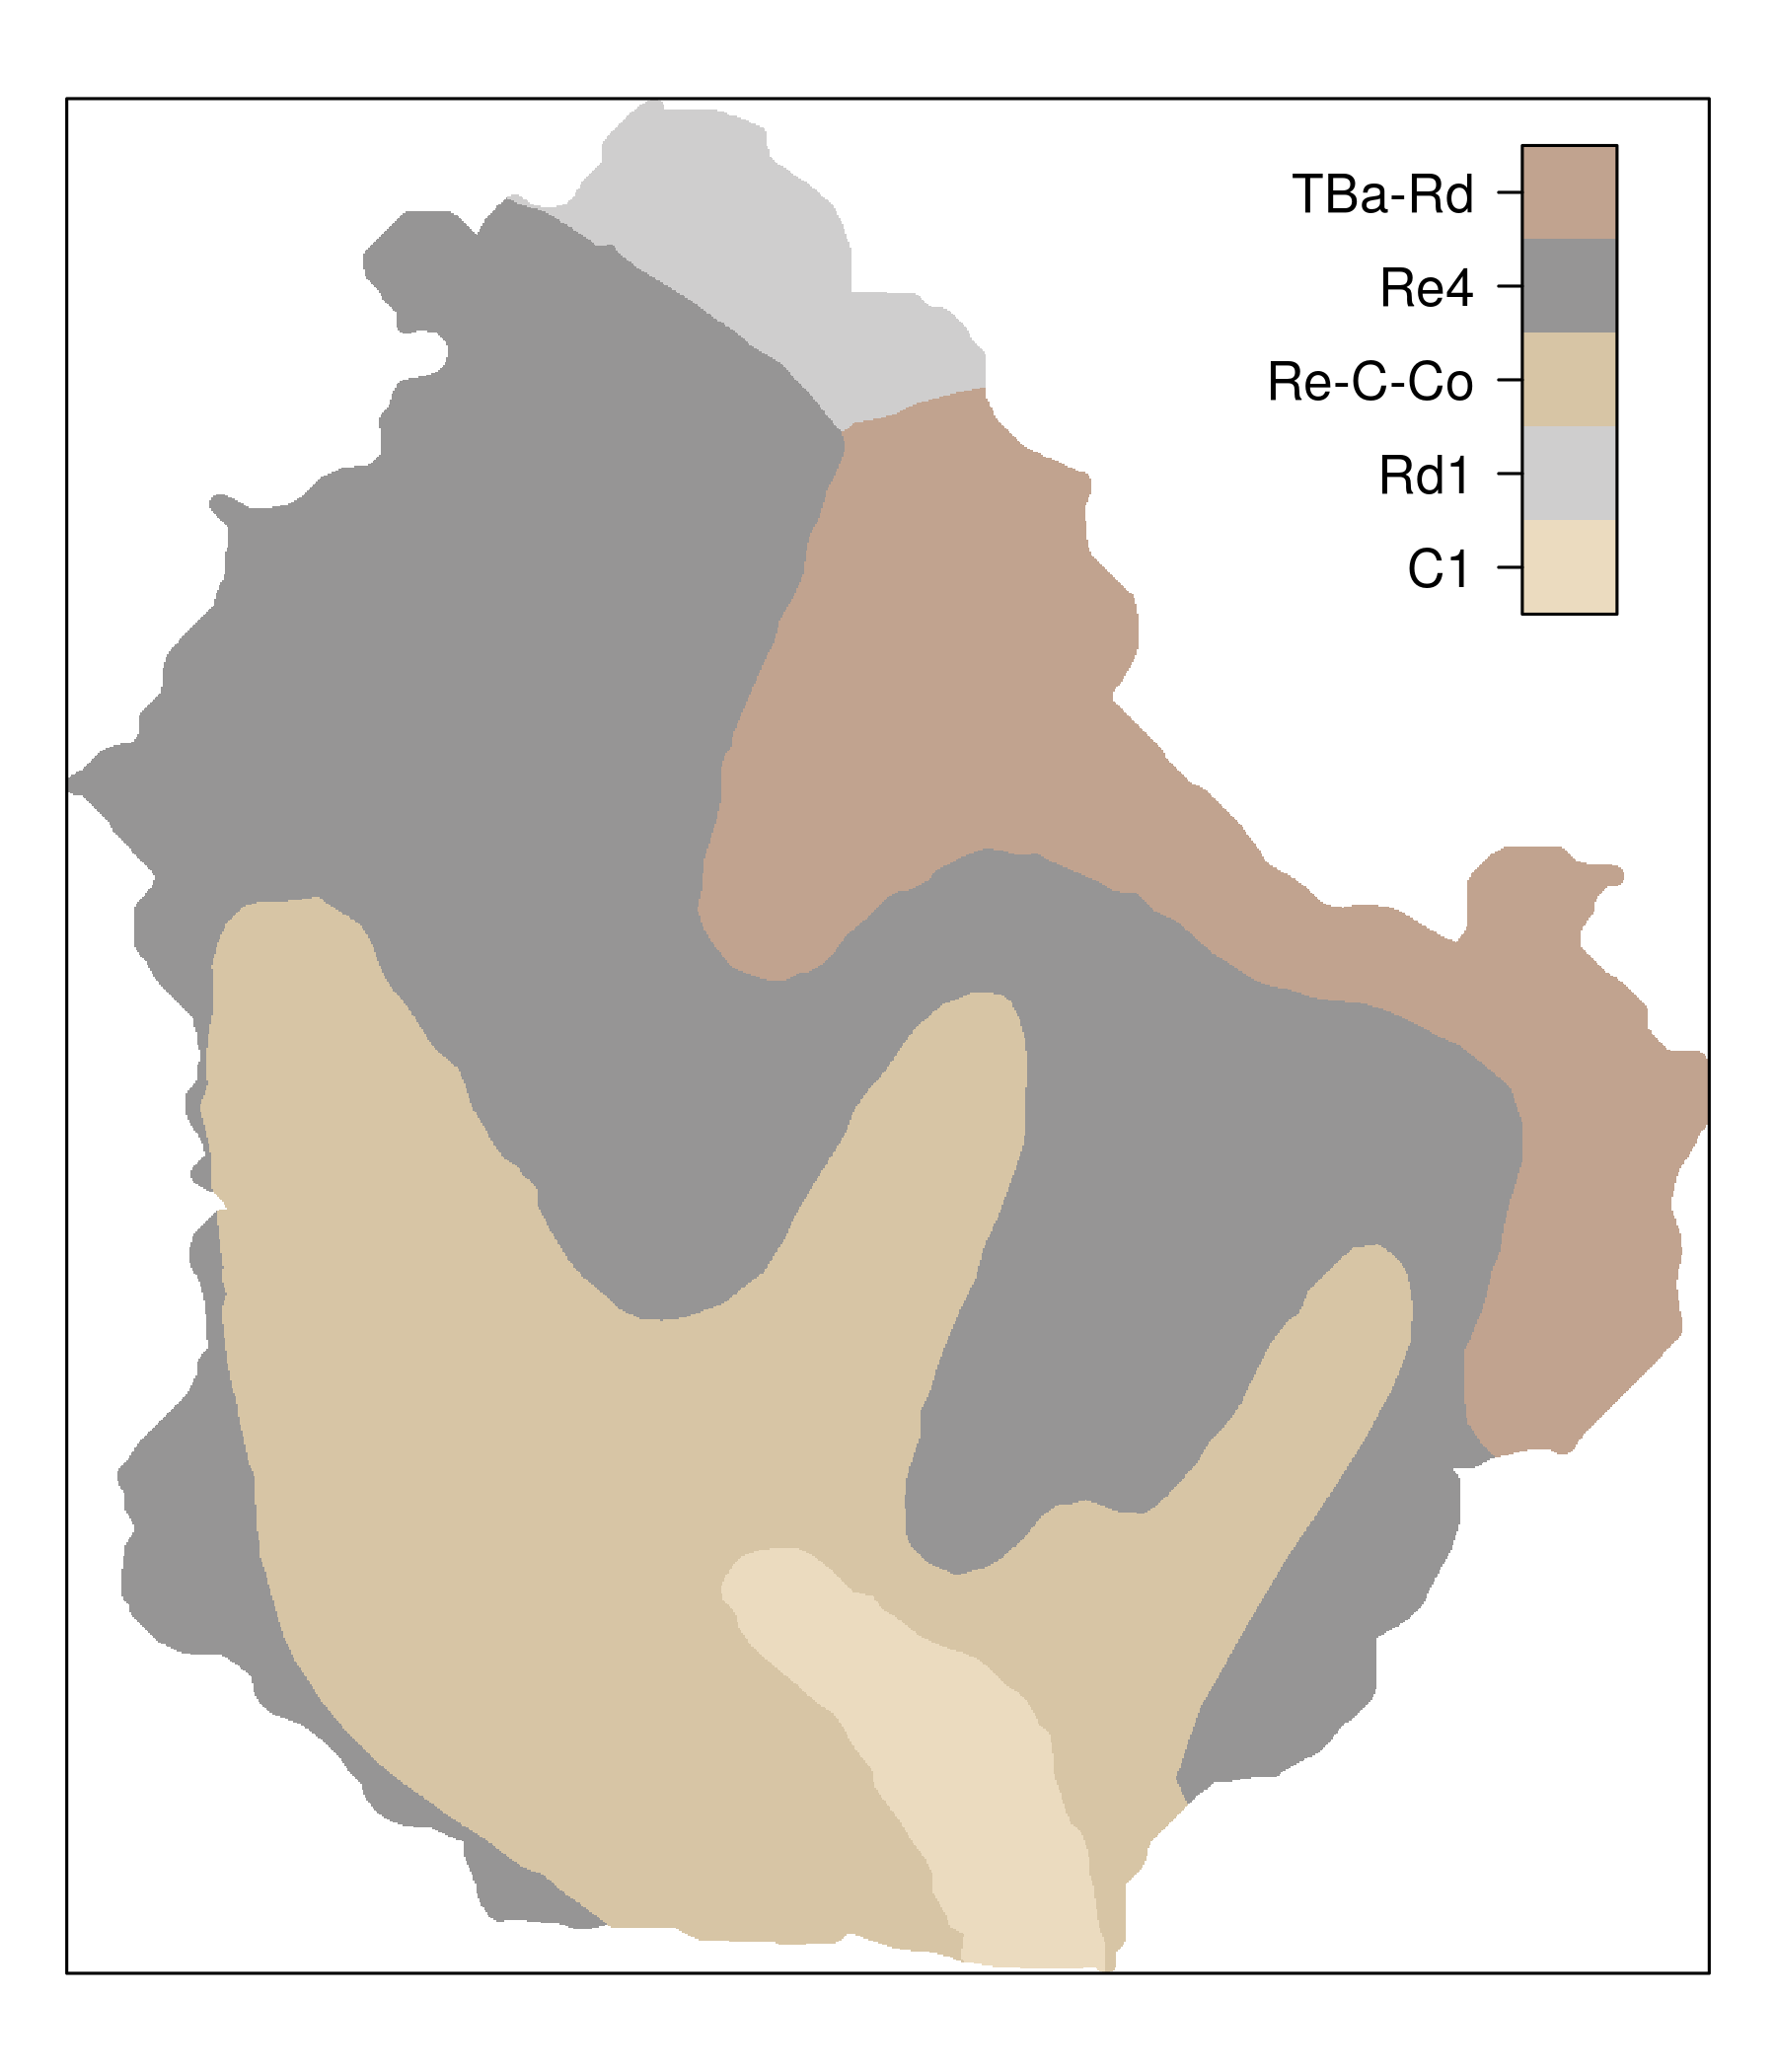
\includegraphics[width = \textwidth]{fig/chap05-soil-old}
\end{minipage}
\begin{minipage}[b]{0.45\textwidth}
\subcaption{}
\centering
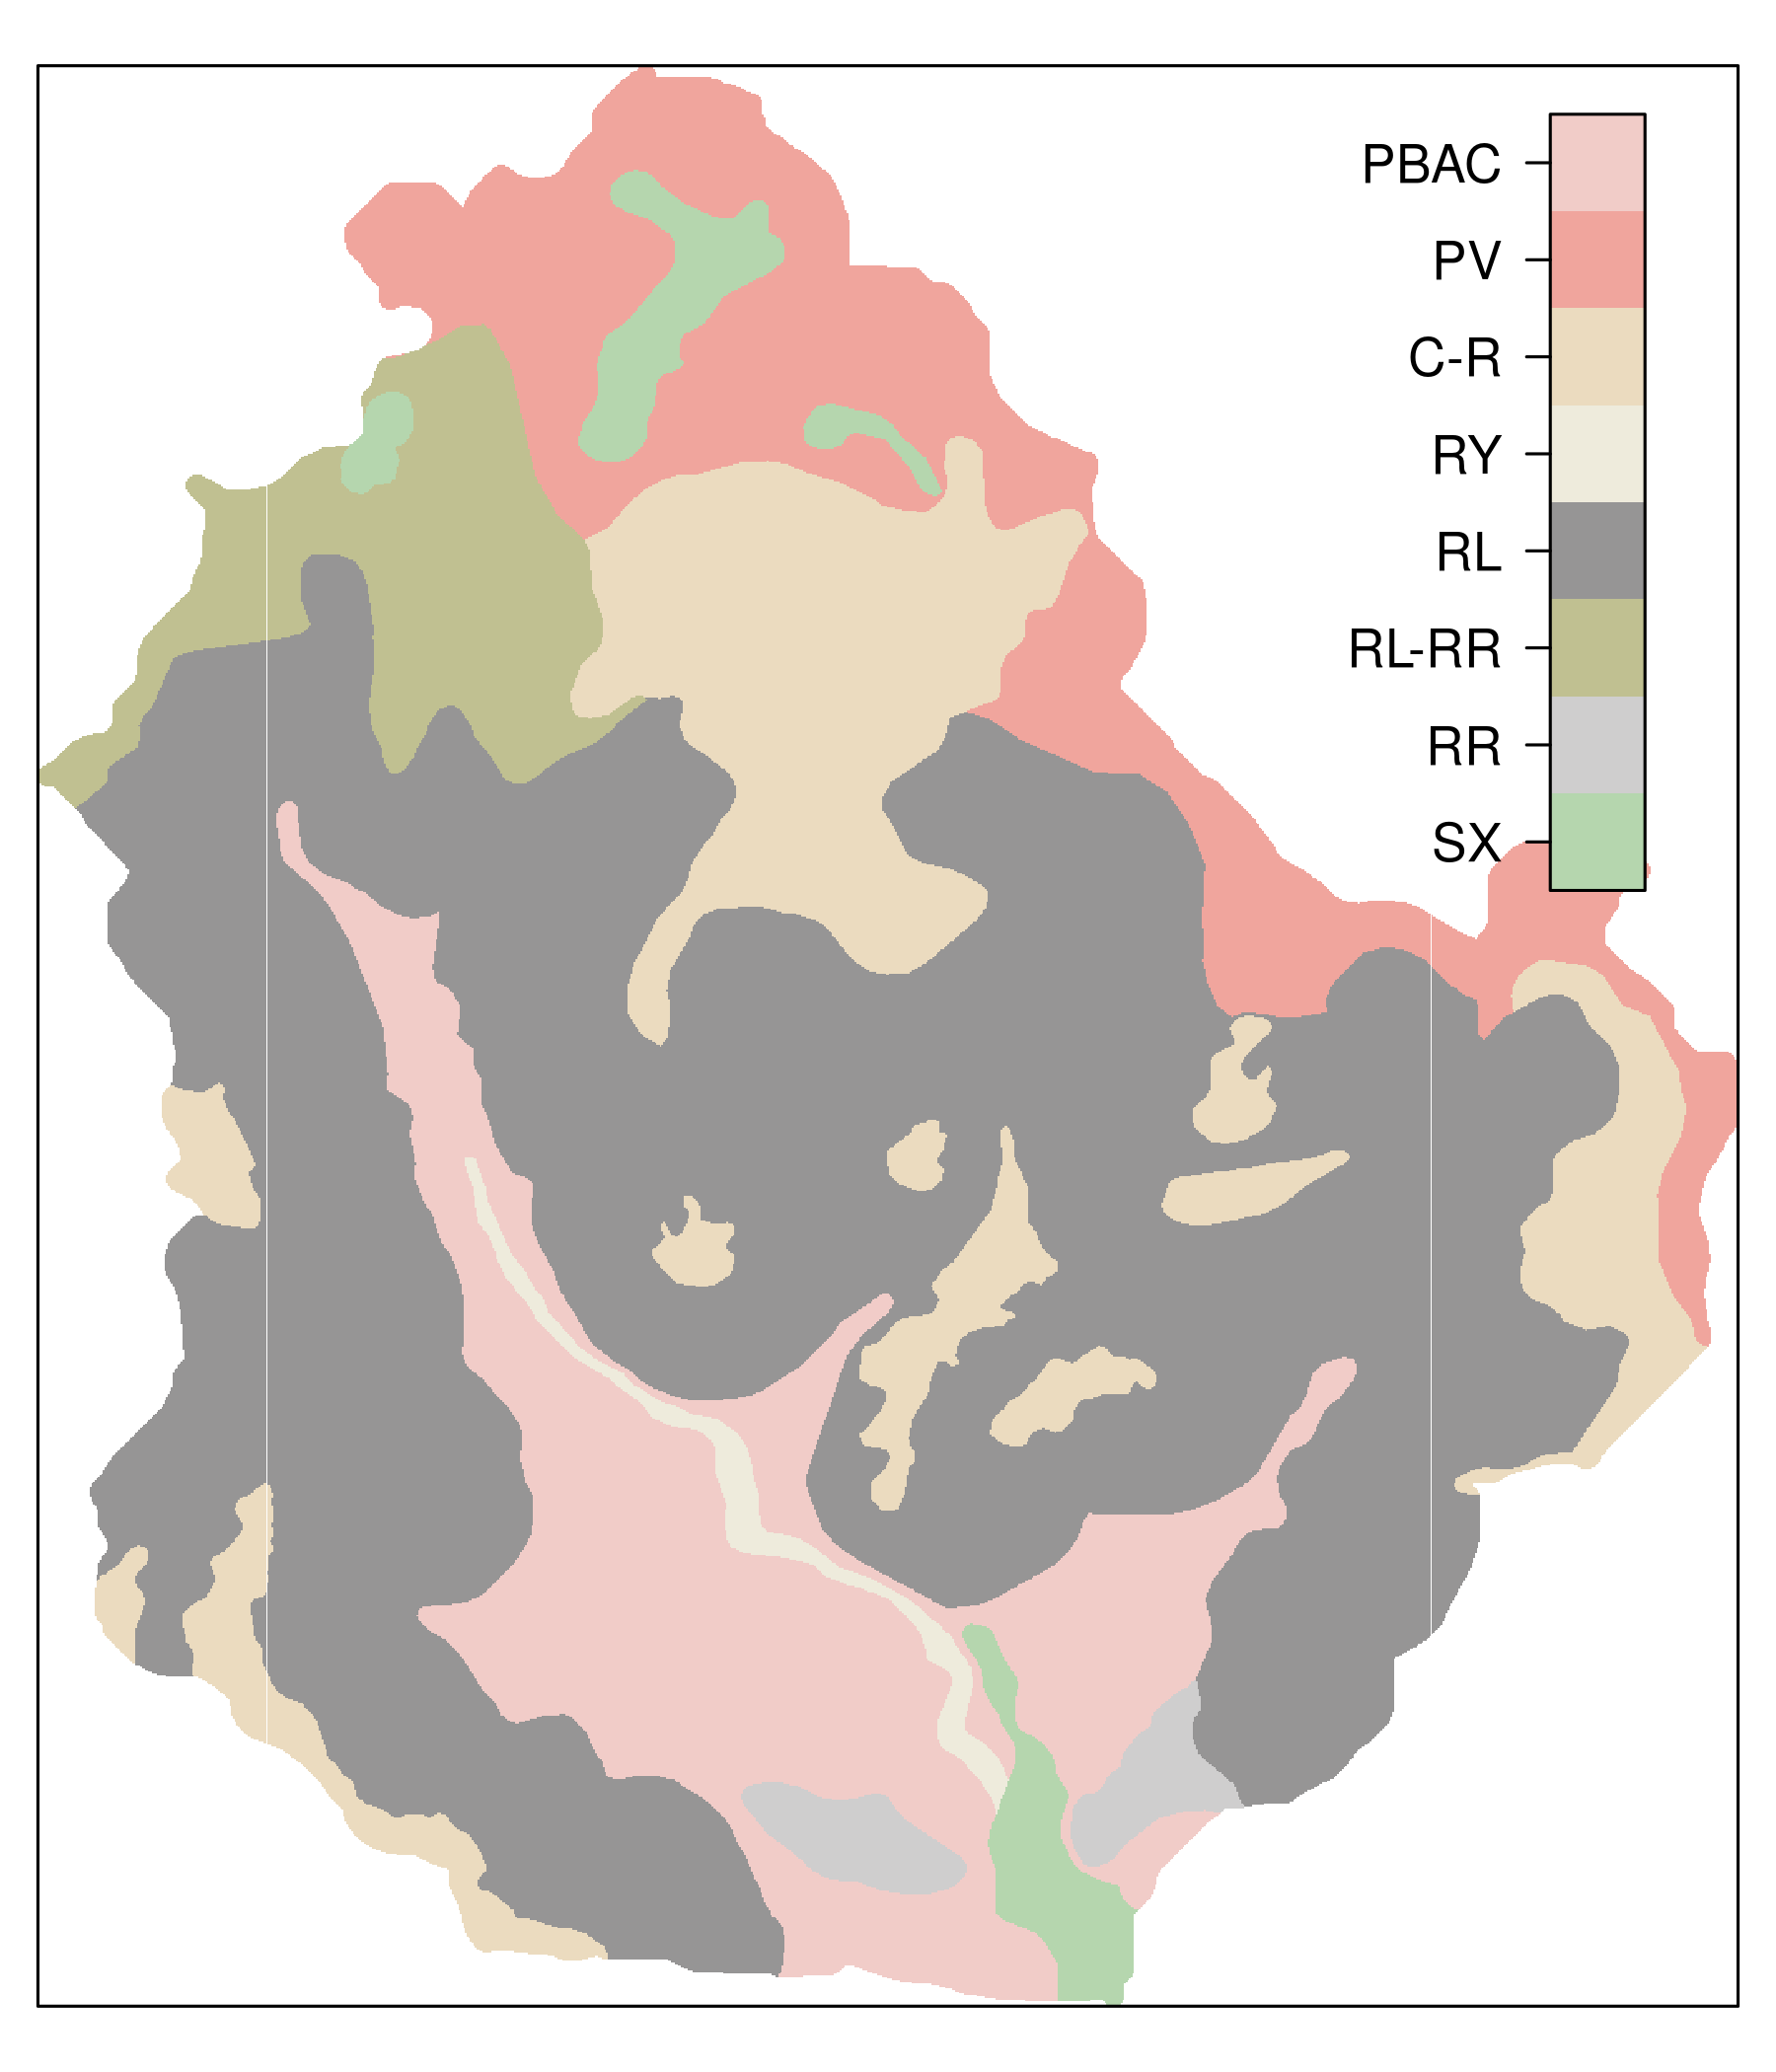
\includegraphics[width = \textwidth]{fig/chap05-soil-new}
\end{minipage} 
\caption[Area-class soil maps included in the Santa Maria dataset.]{Area-class soil maps (a) \soilOld{} and (b) 
\soilNew{} used to derive indicator covariates included in the Santa Maria dataset.}
\label{fig:chap05-soil-maps}
\end{figure}

The second area-class soil map (\soilNew) included in the Santa Maria dataset \cite{Miguel2010} was prepared 
at a \scale{25000}. Satellite images produced by Digital Globe\textregistered{} Quick Bird satellite, freely 
available for visualization in \googleearth, were used to produce the first draft of the soil 
map. Existing area-class soil maps and technical reports \cite{Pedron2005, Poelking2007, Sturmer2008} were 
used to help defining the preliminary soil map legend. Point field observations (soil pits and boreholes) were 
made in 
more than \num{350} locations using a purposive sampling approach (see \autoref{chap:chap04} and 
\autoref{chap:chap07}). These observations helped to identify six modal (representative) soil profiles. Soil 
sampling and description of modal soil profiles, and laboratory analyses of soil samples, followed the standard 
protocols adopted in Brazil \cite{ClaessenEtAl1997, 
SantosEtAl2005}. Soil classification was done following the criteria of the Brazilian System of Soil 
Classification (SiBCS) \cite{SantosEtAl2006}. The final version of the map was prepared using satellite images 
freely available for visualization in \googleearth{} and manually-digitalized topographic sheets 
published at a \scale{25000} \cite{DSG1992a, DSG1992}. Description of soil mapping units includes only the 
most common soil taxon, followed by morphological and laboratory data of modal soil profiles.

The area-class soil maps went through different preprocessing routines. The original \soilOld{} is available 
only in analogical format, what required its digitalization. Georeferencing was carried out using the GDAL 
Georeferencer plug-in in QGIS \cite{GDAL2013, QGIS2013}. Intersections between all meridians and parallels (a 
total of nine) were used as control points to adjust a second order polynomial model. Resampling was performed 
using the cubic resampling method. Soil polygons and their attributes were also manually digitalized in QGIS. 
Because of the coarseness of the cartographic map scale, most geographical markers used to locate validation 
GCPs could not be identified and positional validation was performed using only four GCPs. Estimated error 
statistics suggest that there are large positional errors in all directions, with an RMSE of \SI{114}{\m} and 
a mean azimuth of \SI{128}{\degree} (\autoref{tab:chap05-soil-geo-val}).

\begin{table}[ht]
 \caption[Error statistics of the horizontal positional validation of \soilOld.]{Error statistics of the 
horizontal positional validation of \soilOld{} using $n = 4$ GCPs.}
 \label{tab:chap05-soil-geo-val}
 \centering
 {\small
 \begin{tabular}{lrrrr}
  \hline
  Statistics                   & x-coord & y-coord & Error vector & Azimuth   \\
  \hline
  Mean, \si{\m}                & 30      & -36     & 105          & \ang{128} \\ 
  Absolute mean, \si{\m}       & 58      & 64      & -            & -         \\ 
  Squared mean, \si{\m\square} & 7241    & 5712    & 12953        & -         \\ 
  \hline
 \end{tabular}}
\end{table}

% \begin{figure}[!ht]
%   \centering
%   \includegraphics[width=0.45\textwidth]{azim-soil100}
%   \includegraphics[width=0.45\textwidth]{azim-soil25}
%   \caption{Histogram of the azimuth distribution of the validation of area-class soil maps \soilOld{} 
% and \soilNew{} in the attribute space. Azimuth values were estimated using four and XX
% ground control points located in easily identifiable geographical markers, respectively. 
% The graph was produced using R-package \textit{VecStatGraphs2D}.}
%   \label{fig:soil-azim}
% \end{figure}

The original \soilNew{} is available in digital format in the personal database of the author 
\cite{Miguel2010}. A topology check (Topology Checker plug-in in QGIS) identified that there were many gaps 
and overlaps between polygons. This required a topological edition prior to the use of \soilNew. There also 
was a mismatch between the boundary of \soilNew{} and the actual boundary of the study area as estimated using 
\demNew{} (\autoref{sec:chap05-dem}). This occurred because the database used to produce \soilNew{} 
included \googleearth{} imagery and topographic maps, which are data sources that differ considerably in their 
positional accuracy (\autoref{sec:chap05-dem} and \autoref{sec:chap05-land-use}). To avoid data 
losses, all boundary gaps were manually filled using the closest mapping unit. Boundaries of soil polygons 
were 
defined based on land use (\landNew{}, \autoref{sec:chap05-land-use}) and topographic data (contour lines, 
\autoref{sec:chap05-dem}) as it was done for the original map \cite{Miguel2010}. New delineations were 
checked and approved without modifications by the author of the original map. Because \soilNew{} includes very 
few geographical markers, its positional validation was not possible with the available GCPs. However, the 
RMSE is expected to vary between \SIrange{8}{114}{\m} across the study area as a result of the different 
errors 
present in the data sources used in its production.

Both \soilOld{} and \soilNew{} were cropped to the bounding box of the study area, and resampled to match the 
reference grid using the nearest neighbour resampling method to maintain data integrity. Each category was 
named with the code of the respective mapping unit in the original map. Prior to validation in the attribute 
space, class codes of \soilOld{} were changed to match soil 
taxa codes of the current Brazilian System of Soil Classification using a standard correlation table 
\cite{SantosEtAl2006}. The overall purities of both soil maps are not considerably different. A reason for this 
could be that validation was performed considering only 
the second level of the SiBCS -- it is likely that \soilNew{} would outperform \soilOld{} if validation data 
included soil taxa up to the fourth level of the SiBCS. The low overall purity of \soilOld{} and 
\soilNew{} (\num{31.67} and \SI{30.00}{\percent}, respectively) is likely due to several sources of error. 
First, the small number of modal soil profiles used to produce both maps that might have resulted in an 
optimistic view of the homogeneity of each mapping unit. Second, soil classes of \soilOld{} were translated to 
the more recent SiBCS using only a standard correlation table \cite{SantosEtAl2006} and expert knowledge 
because the survey report does not include analytical soil data. Last, soil classes at the $n = 60$ validation 
sites were inferred in the field using only morphological soil properties and the general concepts of the 
SiBCS.

Five ($p = 5$) covariates were derived from \soilOld{} as described below (including the soil classes according 
to the original and updated classification \cite{AzolinEtAl1988, SantosEtAl2013a}, and the international 
classification \cite{IUSSWorkingGroupWRB2007}):

\begin{description}
 \item[\texttt{SOIL\_100b}] Shallow soil (\textit{Re4}) with low to high base saturation covering mountainous 
 terrain (Solo Litólico Eutrófico/Distrófico relevo montanhoso; Neossolo Litólico Distrófico/Eutrófico;
 Distric/Eutric Leptosol).
  
 \item[\texttt{SOIL\_100c}] Association (\textit{Re-C-Co}) of shallow soil with high base saturation located in
steep terrain (Solo Litólico Eutrófico relevo forte ondulado; Neossolo Litólico Eutrófico; Eutric
 Leptosol), low weathered soil (Cambissolo Eutrófico; Cambissolo Háplico Eutrófico; Eutric Cambisol), and
 colluvial deposits.
  
 \item[\texttt{SOIL\_100d}] Association (\textit{TBa-Rd}) of deep, well-structured, low base saturation soil 
(Terra
 Bruna Estruturada álica; Nitossolo; Nitisol), and shallow soil (Solo Litólico; Neossolo Litólico; Leptosol).
  
 \item[\texttt{SOIL\_100e}] Shallow soil (\textit{Rd1} and \textit{Re4}) with low to high base
 saturation (Solo Litólico Distrófico/Eutrófico; Neossolo Litólico Distrófico/Eutrófico; Distric/Eutric
 Leptosol) located in undulating to mountainous terrain.
  
 \item[\texttt{SOIL\_100f}] This covariate includes the best soil mapping units for row crop agriculture among 
those 
 identified in the soil survey, that is \textit{TBa-Rd}, described above, and \textit{C1}, which is composed
 of low weathered soils developed in lower landscape positions, close to drainage channels (Cambissolo
 Eutrófico; Cambissolo Eutrófico; Eutric Cambisol).
\end{description}

Covariates derived from \soilNew{} are presented below. Mapping unit \textit{RY}, composed mainly of soils 
developed 
from fluvial deposits (Neossolo Flúvico; Fluvisol) does not appear due to the small area that it occupies.

\begin{description}
  \item[\texttt{SOIL\_25a}] Moderately deep soil (\textit{PBAC}) derived from sedimentary rocks, with abrupt 
textural
  change and low base saturation (Argissolo Bruno-Acinzentado; Alisol).
  
  \item[\texttt{SOIL\_25b}] Deep soil (\textit{PV}) derived from igneous rocks, with moderate textural 
gradient,
  and low base saturation (Argissolo Vermelho; Acrisol).
 
  \item[\texttt{SOIL\_25c}] Low weathered soil (Cambissolo Háplico; Cambisol) and shallow soil with low to high 
base
  saturation (Neossolo Litólico/Regolítico Eutrófico/Distrófico; Eutric/Distric Leptosol/Regosol) 
(\textit{C-R}).
 
  \item[\texttt{SOIL\_25d}] Shallow soil (\textit{RL}) with low to high base saturation (Neossolo Litólico 
  Eutrófico/Distrófico; Eutric/Distric Leptosol).
 
  \item[\texttt{SOIL\_25h}] This covariate includes the mapping units with the best soils for row crop 
agriculture
  among those identified in the soil survey (\textit{PBAC}, \textit{PV}, and \textit{SX}). \textit{PBAC} and 
\textit{PV} are as
  described above. \textit{SX} is composed of moderately deep soil derived from sedimentary rocks, with abrupt 
  textural change, low base saturation, and which are saturated with water for long periods of the year 
  (Planossolo Háplico; Planosol).
  
  \item[\texttt{SOIL\_25i}] This covariate includes all three mapping units (\textit{RL}, \textit{RL-RR}, and 
\textit{RR})
  composed mainly of shallow soils (Neossolo Litólico and Neossolo Regolítico; Leptosol and Regosol).
  
  \item[\texttt{SOIL\_25j}] This covariate includes all four mapping units (\textit{PV}, \textit{RL}, 
\textit{RL-RR}, and 
  \textit{C-R}) composed mainly of soil derived from igneous rocks.
\end{description}

\section{DIGITAL ELEVATION MODELS}
\label{sec:chap05-dem}

Two digital elevation models (DEMs) are included in the Santa Maria dataset as sources of terrain covariates. 
The first DEM (\demNew) is the result of the interpolation of the contour lines of the most recent topographic 
sheets produced by the Brazilian 
Army (\scale{25000}) that cover the study area \cite{DSG1980, DSG1992, DSG1992a}. Topographic sheets were 
digitalized
and georeferenced using the GDAL Georeferencer plugin in QGIS. Intersections between all meridians and 
parallels (about \num{160} per topographic sheet) were used as control points to adjust a third order 
polynomial 
model. Resampling was performed using the cubic resampling method. All contour lines, peaks, lakes and rivers, 
and their respective attributes within a distance of \SI{1000}{\metre} from the boundary of the study area 
were manually digitized and stored in vector format. After digitalization, the original coordinate 
reference system (EPSG:31982 -- SIRGAS2000 / UTM zone 22S) of all vector files was transformed to WGS1984 / 
UTM zone 22S (EPSG:32722) using the \Rpackage{rgdal} \cite{BivandEtAl2013a}.

The horizontal positional validation of topographic maps was performed using the $n = 14$ GCPs. According to 
Brazilian 
legislation, high-quality map standards require that at least 90% of the GCPs have horizontal positional errors 
smaller than \SI{13}{\metre}, and an overall horizontal error (i.e. RMSE) smaller than \SI{8}{\metre} at the 
\scale{25000}
\cite{Brasil1984}. Estimated validation statistics show that the overall observed horizontal error 
($\text{RMSE} = \SI{65}{\m}$) 
is larger than those established by current regulations (\autoref{tab:chap05-topomap-geo-val}). The mean error 
vector is larger than \SI{60}{\metre} with an azimuth of \SI{63}{\degree}. Both x- and y-coordinates are 
positively biased, but the largest error occurs in the x-coordinate (\SI{50}{\metre}). Similar ME and MAE 
values suggests that there is a strong systematic positional error. An affine transformation was employed using 
the \Rpackage{vec2dtransf} \cite{Carrillo2012} to correct this systematic error. Model parameters were adjusted 
using the same set of GCPs used for the validation in the geographic space.

\begin{table}[ht]
 \caption[Error statistics of the horizontal validation of topographic maps.]{Error statistics of the 
horizontal validation of topographic maps (\scale{25000}) using $n = 14$  GCPs.}
 \label{tab:chap05-topomap-geo-val}
 \centering
 {\small
 \begin{tabular}{lrrrr}
  \hline
  Statistics                    & x-coord & y-coord & Error vector & Azimuth  \\
  \hline
  Mean, \si{\m}                 & 50      & 27      & 63           & \ang{63} \\ 
  Absolute mean, \si{\m}        & 50      & 32      & -            & -        \\ 
  Squared mean, \si{\m\squared} & 3088    & 1180    & 4268         & -        \\ 
  \hline
 \end{tabular}}
\end{table}

% \begin{figure}[!ht]
%   \centering
%   \includegraphics[width=0.5\textwidth]{azim-car25}
%   \caption{Histogram of the azimuth distribution of the validation of topographic maps in the geographic 
% space. Azimuth values were estimated using 14 ground control points located in easily identifiable 
% geographical markers. 
% The graph was produced using R-package 
% \textit{VecStatGraphs2D}.}
%   \label{fig:topomap-azim}
% \end{figure}

Interpolation of the raster surface with \SI{5}{\metre} grid size was performed using the function 
\texttt{Topo 
to Raster} in ArcGIS\textregistered{} software by ESRI, which includes an interpolation method based on the 
ANUDEM program developed by \citeonline{Hutchinson1989}. Vector files of contour lines (\texttt{multiline}), 
drainage network (\texttt{multiline}), lakes (\texttt{polygons}) and peaks (\texttt{points}) were used to 
generate a 
hydrologically sound DEM, that is, a DEM without spurious depressions and giving a precise representation 
of the hydrological data. Next, the interpolated DEM was imported into GRASS, where a neighbourhood average 
filter was used to remove stair-like artefacts. A window of $7 \times 7$ pixels was used because it removed a 
significant amount of the artefacts and did not affect the derived boundary of the study area (see more 
bellow).

The vertical datum of the DEM was transformed from the local datum to a global datum. The geoidal models 
MAPGEO2010 \cite{IBGE2010a} and EGM1996 \cite{LemoineEtAl1998} were used to calculate the geoidal undulation 
for the local and global datums, respectively. MAPGEO2010 is optimized to estimate geoidal undulations in the 
Brazilian territory, while EGM1996 is a gravitational model of the Earth and is used as the vertical datum for 
Shuttle Radar Topography Mission (SRTM) products. The following equation was used:

\begin{equation}
 h = H + N,
\end{equation}\label{eqn:geoidal}

\noindent where $h$ is the ellipsoidal height (height above the reference ellipsoid that approximates the 
surface of the planet), $H$ is the orthometric height (height above the imaginary surface called geoid and 
commonly referred to as mean sea level), and $N$ is the geoidal undulation. Ellipsoidal heights estimated by 
MAPGEO2010 are referenced to the world ellipsoid of 1980, while EGM1996 estimates ellipsoidal heights 
referenced to the world ellipsoid of 1984. Because the difference between both ellipsoids is of the order of 
millimetres, it can be assumed that both models estimate the same ellipsoidal height. Therefore, if 
$h_{\text{EGM1996}} = h_{\text{MAPGEO2010}}$, then orthometric heights referenced to the local vertical datum 
can be transformed to the global vertical datum using the following equation:

\begin{equation}
 H_{\text{EGM1996}} = H_{\text{MAPGEO2010}} + N_{\text{MAPGEO2010}} - N_{\text{EGM1996}}.
\end{equation}

\noindent The difference in the geoidal undulation estimated by both models is of about one meter in the 
entire study area. Thus, transforming the vertical datum was done adding one meter to the raster surface 
interpolated from contour lines, yielding the first DEM included in the Santa Maria dataset (\demNew{}).

The second DEM (\demOld{}) is the well known SRTM DEM ($\SI{3}{\arcsecond} \approx \SI{90}{\m}$ spatial 
resolution) produced by the National Aeronautics and Space Administration’s Jet Propulsion Laboratory in 
collaboration with the National Geospatial\-/Intelligence Agency \cite{RodriguezEtAl2006}. The SRTM DEM version 
used here is the \emph{sink\-/filled SRTM version \num{4}}, prepared by the Consultative Group for 
International Agricultural Research (\cgiar) using the same hydrologically correct interpolation method that 
was used above to produce \demNew{} \cite{ReuterEtAl2007, JarvisEtAl2008}. However, the only data source used 
was the SRTM DEM version 3 converted to point data.

The SRTM DEM was processed to match the reference grid using cubic resampling (\gdal{gdalwarp} and 
\grass{r.resamp.interp}). This resampling method was used because it is efficient in minimizing the 
double-oblique stripping present in SRTM products \cite{Samuel-RosaEtAl2013c}. Sinks produced during datum 
transformation were filled using the \grass{r.fill.dir}. Vertical datum transformation was not necessary 
because elevation values of the SRTM DEM already are referenced to the global geoid model EGM1996 
(orthometric heights). These DEMs were used to derive the terrain covariates used in the thesis. 

\begin{figure}[!ht]
\centering
\begin{minipage}[b]{0.45\textwidth}
\subcaption{}
\centering
\includegraphics[width = \textwidth]{fig/chap05-dem-old}
\end{minipage}
\begin{minipage}[b]{0.45\textwidth}
\subcaption{}
\centering
\includegraphics[width = \textwidth]{fig/chap05-dem-new}
\end{minipage} 
\caption[Digital elevation models included in the Santa Maria dataset.]{Digital elevation models (a) \demOld{} 
and (b) \demNew{} used to derive terrain covariates included in the Santa Maria dataset.}
\label{fig:chap05-dem}
\end{figure}

A third DEM was included with the sole purpose of supporting the orthorectification -- removal of the effects 
of the perspective of the sensor on the relative position of objects in the image -- and topographic correction 
-- removal of the effects of the topography on the reflectance values, i.e. on the illumination of the 
geomorphic surfaces -- of satellite images (\autoref{sec:chap05-sat-image}) \cite{Mather2004, 
Schowengerdt2007}. The third DEM (\topodata) was produced by the Brazilian National Institute for Space 
Research (\inpe) by refining the SRTM DEM version 1 (\q{unfinished}) to $\SI{1}{\arcsecond} \approx 
\SI{30}{\m}$ spatial resolution using ordinary kriging with a Gaussian spatial autocorrelation model 
\cite{ValerianoEtAl2012}. Eight tiles were mosaicked (\gdal{gdal\_translate}) and the CRS transformed from 
WGS1984 (EPSG:4326) to WGS1984 / UTM zone 22S (EPSG:32722) using cubic resampling (\gdal{gdalwarp}), and the 
sinks filled using \grass{r.fill.dir}. Before the atmospheric correction of satellite images, orthometric 
heights were converted to ellipsoidal heights using \autoref{eqn:geoidal}, the geoidal undulation calculated 
with the gravitational model EGM1996. This conversion was done because orbital satellites use the WGS1984 
ellipsoid as vertical datum. For the orthorectification of satellite images, the DEM was then processed using 
\grass{r.resamp.interp} with the bicubic resampling method to match the reference grid.

The three DEMs present similar vertical accuracy (\autoref{tab:chap05-dem-attr-val}). In the case of \demNew{}, 
which was derived from contour lines published at a \scale{25000}, the vertical positional accuracy does not 
meet the high-quality standards of current Brazilian legislation, which states that 90% of the GCPs should have 
vertical errors smaller than \SI{5}{\metre}, which is half of the distance between contour lines 
\cite{Brasil1984}. The corresponding RMSE should be less than \SI{3}{\metre}.

\begin{table}[ht]
 \caption[Error statistics of the vertical validation of \demOld, TOPODATA, and \demNew.]{Error statistics of 
the vertical validation of \demOld, TOPODATA, and \demNew{} using $n = 60$ validation points located along $m = 
12$ linear transects.}
 \label{tab:chap05-dem-attr-val}
 \centering
 {\small
 \begin{tabular}{lrrrrrr}
  \hline
  Statistics                   & \demOld{} & TOPODATA & \demNew{} \\
  \hline
  Mean, \si{\m}                & -15       & -17      & -16       \\ 
  Absolute mean, \si{\m}       & 15        & 17       & 16        \\ 
  Squared mean, \si{\m\square} & 350       & 361      & 374       \\ 
  \hline
 \end{tabular}}
\end{table}

% Figure \ref{fig:cdf-elev} shows that estimated validation statistics have different cumulative 
% distribution functions (CDF). The estimates are more uniformly distributed along the interval of 
% values for \texttt{ELEV\_10} than for \texttt{ELEV\_90} and \texttt{ELEV\_30}. While 
% \texttt{ELEV\_10} has a 50\% probability that absolute errors are below 15 m, \texttt{ELEV\_90} has 
% a 70\% probability that absolute errors are below 15 m. This suggests that the accuracy of 
% \texttt{ELEV\_90} is very consistent across the study area, with a few extreme values, while the 
% accuracy of \texttt{ELEV\_10} have a stronger spatial variation. For \texttt{ELEV\_30}, the 
% interpolation method used to refine the original SRTM DEM to 30 m \cite{ValerianoEtAl2012} seems to 
% have produced a spatial redistribution of the errors.

% \begin{figure}[!ht]
%   \centering
%   \includegraphics[width=0.9\textwidth]{fig/cdf-ELEV-90} 
%   \includegraphics[width=0.9\textwidth]{fig/cdf-ELEV-30}
%   \includegraphics[width=0.9\textwidth]{fig/cdf-ELEV-10}
%   \caption{Cumulative distribution functions of mean error, mean absolute error, and squared error of 
% elevation values estimates by digital elevation models \texttt{ELEV\_90}, \texttt{ELEV\_30}, and 
% \texttt{ELEV\_10}.}
%   \label{fig:cdf-elev}
% \end{figure}

Despite all DEMs present a similar vertical accuracy, \demNew{} is considered the highest quality DEM in the 
Santa Maria dataset. Because it was produced using information about the drainage network and location of lakes 
and natural depressions, it is likely to provide a better hydrological representation of the study area. As 
such, \demNew{} was used to estimate the geographical limits (boundary) of the catchment that constitute the 
study area, for which GRASS modules \texttt{r.watershed} and 
\texttt{r.water.outlet} were employed. Because the overall deviation between the affine-corrected coordinates 
of topographic maps and target coordinates of GCPs is $\text{RMSE} = \SI{29.55}{\m}$ -- there still is 
uncertainty about the correct position of topographic maps -- a \SI{30}{\m} buffer was added to the 
geographical limits of the catchment. The water outlet point used to estimate the boundary is located on the 
bridge that crosses the main drainage channel (\ang{-29.65868}, \ang{-53.78969}).

Eight terrain attributes were derived from each of \demOld{} and \demNew{} to produce the covariate data 
included in the Santa Maria dataset, the first of them being elevation (\texttt{ELEV}). The others are slope, 
aspect, northernness, flow accumulation, topographic wetness index, stream power index, and topographic 
position index.

Slope (\texttt{SLP}) and aspect (\texttt{ASP}) were calculated using \grass{r.param.scale}. This module 
calculates 
terrain attributes by fitting a bivariate quadratic polynomial using least squares \cite{Wood1996}. It allows 
using different window sizes to fit the bivariate quadratic polynomial, thus including the effect of scale in 
the calculation of terrain attributes. Seven window sizes were used (3, 7, 15, 31, 63, 127, and 255) and the 
results for calculated slope can be seen in \autoref{fig:chap05-slope}. Larger window sizes result in a 
smoother version of the terrain attribute, while smaller windows sizes result in raster maps with more 
(small-scale) details. Several flat surfaces (slope of \ang{0}) were produced in the slope raster maps 
calculated using \texttt{ELEV\_90} as a result of resampling the original DEM from \num{90} to \SI{5}{\m}. A 
value of \ang{0.1} was added to the rasters to remove these flat surfaces.

\begin{figure}[!ht]
\centering
\includegraphics[width = 0.90\textwidth]{fig/chap05-slope}
\caption[Slope derived using windows of different sizes.]{Slope \texttt{SLP} raster surfaces derived from 
\demNew{} using windows of sizes (from left to right) $3 \times 3$, $31 \times 31$, $127 \times 127$, and $255 
\times 255$.}
\label{fig:chap05-slope}
\end{figure}

Aspect values had to be corrected before use because \grass{r.param.scale} stores aspect values in the range 
\SIrange{0}{+180}{\degree} from West to North to East, and \SIrange{0}{-180}{\degree} from West to South to 
East, when the standard procedure is to work with aspect values ranging from \SIrange{0}{360}{\degree} 
clockwise. This correction was done using

\begin{equation}
 \texttt{ASP}_{0} =
 \begin{cases}
  \texttt{ASP}_{GRASS} + \ang{360} & \text{if}\;\; \texttt{ASP}_{GRASS} < \ang{0}, \\
  \texttt{ASP}_{GRASS}             & \text{else},
 \end{cases}
\end{equation}

\noindent and

\begin{equation}
 \texttt{ASP} =
 \begin{cases}
  \texttt{ASP}_{0} + \ang{270} & \text{if}\;\; \texttt{ASP}_{0} < \ang{90}, \\
  \texttt{ASP}_{0} - \ang{90}  & \text{else}.
 \end{cases}
\end{equation}

\noindent A second correction of aspect values involved their linearization. This is necessary because aspect 
is a circular variable, that is, the beginning (\ang{0}) and end (\ang{360}) of the measurement scale have the 
same physical meaning. Aspect values were transformed to northernness (\texttt{NOR}), a measure of the degree 
of exposition of a given surface to the North, a linear variable, using the equation

\begin{equation}
 \texttt{NOR} = abs(\ang{180} - \texttt{ASP}).
\end{equation}\label{eq:NOR}  

Flow accumulation (ACC), also known as catchment area or contributing area, was calculated using 
\grass{r.watershed}, the resulting raster surface being multiplied by the square of the cell size (i.e. by the 
cell area \SI{\approx25}{\metre\square}) to convert to areal units. This raster surface was used to calculate 
the topographic wetness index (\texttt{TWI}) and the stream power index (\texttt{SPI}) using

\begin{equation}
 \text{sACC} = \dfrac{\text{ACC}}{5},
\end{equation}\label{eq:sACC}

\begin{equation}
 \texttt{TWI} = log \dfrac{\text{sACC}}{tan(\texttt{SLP})},
\end{equation}\label{eq:TWI}

\noindent and

\begin{equation}
 \texttt{SPI} = log(\text{sACC} \times tan(\texttt{SLP})),
\end{equation}\label{eq:SPI}

\noindent where sACC is the specific catchment area, \SI{5}{\m} is the cell size, and \texttt{SLP} is the 
slope 
raster surface calculated using seven different window sizes.

The topographic position index \texttt{TPI} was calculated with \saga{ta\_morphometry}. Different values of 
maximum radius were used to include the effect of scale, all of them related to the window sizes used to 
calculate previous terrain attributes. A minimum radius value of \SI{3}{\m} was used in all calculations.

A total of $1 \times \texttt{ELEV} + 7 \times (\texttt{NOR}, \texttt{SLP}, \texttt{TWI}, \texttt{SPI}, 
\texttt{TPI}) = 36$ covariates 
were defined using the terrain attributes derived from \demOld{} and \demNew{}.

\section{GEOLOGIC MAPS}
\label{sec:chap05-geo-maps}

Geologic data comes from the two most recent geologic maps (\geoOld{} and \geoNew{}) published at the 
\scales{50000}{25000} \cite{GasparettoEtAl1988, MacielFilho1990} (\autoref{fig:chap05-geo-maps}). Both of 
them were produced based on the most recent topographic sheets produced by the Brazilian Army at the 
\scales{50000}{25000} \cite{DSG1980, DSG1992, DSG1992a}. Alike topographic maps, geologic maps were 
available only in analogical format, and were hand digitized and georeferenced in QGIS. Intersections 
between all meridians and parallels ($n = 16$) were used as control points to adjust a second order polynomial 
model. Resampling was performed using the cubic resampling method. The original CRS 
(EPSG:31982 -- SIRGAS2000 / UTM zone 22S) was transformed to match the reference grid using the 
\Rpackage{rgdal} \cite{BivandEtAl2013a}.

\begin{figure}[!ht]
\centering
\begin{minipage}[b]{0.45\textwidth}
\subcaption{}
\centering
\includegraphics[width = \textwidth]{fig/chap05-geo-old}
\end{minipage}
\begin{minipage}[b]{0.45\textwidth}
\subcaption{}
\centering
\includegraphics[width = \textwidth]{fig/chap05-geo-new}
\end{minipage} 
\caption[Geologic maps included in the Santa Maria dataset.]{Geologic maps (a) \geoOld{} and (b) \geoNew{} used 
to derive indicator covariates included in the Santa Maria dataset.}
\label{fig:chap05-geo-maps}
\end{figure}

The positional validation of geologic maps was performed using $n = 8$ (\geoOld{}) and $n = 5$ (\geoNew{}) 
GCPs, respectively. Validation statistics show that the positional accuracy of neither geologic map meets the 
high-quality standards of the current Brazilian legislation (\autoref{tab:chap05-geology-geo-val}). Estimated 
RMSE are \num{147} and \SI{69}{\m} for \geoOld{} and \geoNew{}, respectively, when the maximum RMSE accepted 
are \num{25} and \SI{13}{\m}, respectively. For \geoOld{}, the lowest accuracy is found in the y-coordinate, 
while for \geoNew{}, the x-coordinate is the least accurate. Validation statistics suggest that there is a 
strong systematic error, which probably was propagated from the topographic maps used to produce the geologic 
maps. Therefore, the same strategy (affine transformation) used to remove the systematic positional error of 
the topographic maps was employed on geologic maps. Due to the lack of GCPs, model parameters were adjusted 
using the same set of GCPs used for the validation. The estimated uncertainty (RMSE) of the affine 
transformation is \num{86} and \SI{22}{\m} for \geoOld{} and \geoNew{}, respectively.

\begin{table}[ht]
 \caption[Error statistics of the horizontal validation of geologic maps.]{Error statistics of the horizontal 
validation of geologic maps \geoOld{} and \geoNew{} using $n = 8$ and $n = 5$ GCPs.}
 \label{tab:chap05-geology-geo-val}
 \centering
 {\small
 \begin{tabular}{lrrrr}
  \hline
  Statistics                   & x-coord & y-coord & Error vector & Azimuth   \\
  \hline
  \multicolumn{5}{l}{\geoOld{} ($n = 8$)}                                     \\
  \hline
  Mean, \si{\m}                & 10      & -102    & 140          & \ang{169} \\ 
  Absolute mean, \si{\m}       & 43      & 125     & -            & -         \\ 
  Squared mean, \si{\m\square} & 3431    & 18067   & 21498        & -         \\
  \hline
  \multicolumn{5}{l}{\geoNew{} ($n = 5$)}                                     \\
  \hline
  Mean, \si{\m}                & 51      & 29      & 67           & \ang{58}  \\ 
  Absolute mean, \si{\m}       & 51      & 29      & -            & -         \\ 
  Squared mean, \si{\m\square} & 3457    & 1312    & 4769         & -         \\
  \hline
 \end{tabular}}
\end{table}

% \begin{figure}[ht]
%  \centering
%  \caption{Histogram of the azimuth distribution of the validation of geologic maps 
%  \texttt{GEO\_50} (left) and \texttt{GEO\_25} (right) in the geographic space. Azimuth values were 
%  estimated using, respectively, eight and five ground control points located in easily identifiable 
% geographical 
%  markers. The graph was produced using \Rpackage{VecStatGraphs2D}.}
%  \label{fig:chap05-geology-azim}
% \end{figure}

Three ($p = 3$) covariates were derived from \geoOld{}:

\begin{description}
 \item[\texttt{GEO\_50a}] Inferior Sequence of the Serra Geral Formation. Composed mainly by basic 
 igneous rocks (tholeiitic basalt and andesite). It is likely related to high soil clay content and effective 
cation exchange capacity;
 
 \item[\texttt{GEO\_50b}] Superior Sequence of the Serra Geral Formation. Composed mainly by acid 
 igneous rocks (granophyric rhyolite and rhyodacite). It is likely related to moderate to 
 high \texttt{CLAY} and \texttt{ECEC};
 
 \item[\texttt{GEO\_50c}] Botucatu Formation. Composed mainly by aeolian sandstones. It is likely  related to 
low \texttt{CLAY} and \texttt{ECEC};
\end{description}

Four ($p = 4$) covariates were derived from \geoNew{}, the first three of them having the same meaning 
of those derived from \geoOld{}:

\begin{description}
 \item[\texttt{GEO\_25a}] Inferior Sequence of the Serra Geral Formation;
 
 \item[\texttt{GEO\_25b}] Superior Sequence of the Serra Geral Formation;
 
 \item[\texttt{GEO\_25c}] Botucatu Formation;
 
 \item[\texttt{GEO\_25d}] Quaternary deposits of fluvial, alluvial, and colluvial origin. It can help 
explaining the low clay content in areas where the soil is believed to have developed from igneous rocks as 
depicted in less detailed geologic maps.
\end{description}

\section{LAND USE MAPS}
\label{sec:chap05-land-use}

The first land use map used to derive covariate data included in the Santa Maria dataset was produced by 
manually digitizing land use data of \num{1980} (\landOld{}) published in the most recent 
topographic map produced by the Brazilian Army (\scale{25000}) \cite{DSG1992a, DSG1992}. Most processing 
steps, including the correction of positional bias, are described in \autoref{sec:chap05-dem}, except for 
the use of the nearest neighbour resampling method to match \landOld{} to the reference grid.

\begin{figure}[!ht]
\centering
\begin{minipage}[b]{0.45\textwidth}
\subcaption{}
\centering
\includegraphics[width = \textwidth]{fig/chap05-land-old}
\end{minipage}
\begin{minipage}[b]{0.45\textwidth}
\subcaption{}
\centering
\includegraphics[width = \textwidth]{fig/chap05-land-new}
\end{minipage}
\begin{minipage}[b]{0.45\textwidth}
\subcaption{}
\centering
\includegraphics[width = \textwidth]{fig/chap05-land-diff}
\end{minipage}
\caption[Land use maps included in the Santa Maria dataset.]{Land use maps (a) \landOld{} and (b) \landNew{} 
used to derive indicator covariates included in the Santa Maria dataset such as (c) \texttt{LUdiff}, the land 
use change between the years of 1980 and 2009.}
\label{fig:chap05-land-use}
\end{figure}

The second land use map (\landNew{}) was prepared at a \scale{2000} using high resolution (\SI{2.4}{\m}) 
Quickbird satellite images of \num{2008} and \num{2009}, made publicly available in \googleearth{} 
\cite{SamuelRosaEtAl2011a}. Identification of land uses and delineation of mapping units were done manually, on 
the computer screen, without using any automated classification routine. Positional validation of 
\googleearth{} imagery revealed that they have only minor systematic positional errors 
(\autoref{tab:chap05-google-geo-val}). Despite this, the attribute validation of both land use maps, using $n = 
60$ validation points placed along $m = 12$ linear transects, showed that they have similar overall accuracy 
close to \SI{70.00}{\percent}.

\begin{table}[ht]
 \caption[Error statistics of the horizontal validation of \googleearth{} imagery.]{Error statistics of the 
horizontal validation of \googleearth{} imagery using $n = 14$ GCPs.}
 \label{tab:chap05-google-geo-val}
 \centering
 {\small
 \begin{tabular}{lrrrr}
  \hline
  Statistics                   & x-coord & y-coord & Error vector & Azimuth   \\
  \hline
  Mean, \si{\m}                & -1      & 3       & 6            & \ang{184} \\ 
  Absolute mean, \si{\m}       & 3       & 5       & -            & -         \\ 
  Squared mean, \si{\m\square} & 14      & 57      & 71           & -         \\ 
  \hline
 \end{tabular}}
\end{table}

\landOld{} was used to derive $p = 2$ covariates defined as indicator variables, with plantation forests 
(\textit{PF}) and human settlements (\textit{S}) being grouped together due to their small importance in terms 
of 
covered area (\textit{PF}) and for not containing any soil observation (\textit{S}). These covariates are:

\begin{description}
 \item[\texttt{LU1980a}] Native forest (\textit{FS}), which is likely to have soils with higher fertility.
  
 \item[\texttt{LU1980b}] Animal husbandry (\textit{H}), the second most important land use in the study area, 
which is
 likely to have a soil fertility status lower than native forests.
\end{description}

Four ($p = 4$) indicator covariates were derived from \landNew{}, with plantation forests (\textit{PF}), human 
settlements (\textit{S}), and other land uses (\textit{O}), which comprise natural and artificial water bodies, 
being 
grouped together due to their small importance in terms of covered area (\textit{PF}) and for not containing 
any 
soil observation (\textit{S} and \textit{O}). These covariates are:

\begin{description}
 \item[\texttt{LU2009a}] Native forest (\textit{FS}), as described above.
 
 \item[\texttt{LU2009b}] Shrubland (\textit{SS}), which is likely to have a soil fertility level above those 
found in
 areas used with annual crop agriculture and animal husbandry, but lower than in native forests.
 
 \item[\texttt{LU2009c}] Animal husbandry (\textit{H}), as described above.
  
 \item[\texttt{LU2009d}] Annual crop agriculture (\textit{AA}), which is likely to present the lowest soil 
fertility 
 levels due to the usually poor management practices employed.
\end{description}

A seventh indicator covariate (\texttt{LUdiff}) was derived using data from both land use maps. It consists of 
the 
land use change between \num{1980} and \num{2009}, computed by checking if the land use has changed (1) or 
remained the same (0) in every grid cell after the 29-year period. \texttt{LUdiff} can be useful, for example, 
to 
explain the low soil organic carbon content in forest soils due to previous use with crop agriculture or animal 
husbandry.

\section{SATELLITE IMAGES}
\label{sec:chap05-sat-image}

Two sources of satellite images were used to produce covariate data included in the Santa Maria dataset. The 
first is the Thematic Mapper (TM) sensor aboard the longest-operating Earth observation satellite -- Landsat 5. 
The satellite image used was acquired on \num{26} December \num{2010} and is freely available in the database 
of the Division of Image Generation of the Brazilian National Institute for Space Research (\inpedgi). The 
image contains seven spectral bands (\autoref{tab:chap05-satellites}) (including a thermal band that is not 
included in the Santa Maria dataset), with \SI{8}{\bit} radiometric resolution (digital numbers from 
\numrange{0}{255}) and \SI{30}{\m} spatial resolution. The satellite image was orthorectified using 
Geomatica\textregistered{} OrthoEngine\textregistered{} with the Landsat rigorous model (Toutin's Model) 
\cite{Toutin2004, PCIGeomatics2007}. Due to the absence of good identifiable field GCPs, $n = 28$ GCPs were 
collected from \googleearth{} imagery, which have a high positional accuracy in the study area 
(\autoref{tab:chap05-google-geo-val}). GCPs were located 
at easily identifiable geographical markers such as road intersections and bridges, evenly distributed 
throughout the image, and covering a variety of elevations, following standard recommendations 
\cite{PCIGeomatics2007}. 
% TODO: add link to \autoref{fig:chap05-ortho-gcps}
The DEM used for orthorectification is TOPODATA after preprocessing as described in \autoref{sec:chap05-dem}. 
Resampling was done using the nearest neighbour method to avoid changing the digital numbers.

After orthorectification, all bands were imported into GRASS, where all other necessary corrections were 
performed. Radiometric correction (conversion from digital numbers to top-of-atmosphere reflectance) was done 
using \grass{i.landsat.toar}. Atmospheric correction (removal of the effects of the atmosphere on the 
reflectance values) was done with the 6S atmospheric model \cite{VermoteEtAl1997} as implemented in 
\grass{i.atcorr} using the tropical atmospheric model, the continental aerosols model, an image-based 
visibility estimate of \SI{20}{\km}, and a constant elevation of \SI{300}{\m}.

The second source of satellite images is RapidEye. Images are available through the Brazilian Ministry of the 
Environment \cite{Brasil2012}, which has a full coverage of the Brazilian territory for \num{2011} and 
\num{2012}. The satellite image used (tile number \num{2225403}) was acquired on \num{16} November \num{2012} 
(second coverage). It contains five spectral bands 
(\autoref{tab:chap05-satellites}), featuring among them the so-called red-edge band, located between the red 
and the near-infrared bands. This spectral band is the main feature distinguishing RapidEye images from most 
other sources of satellite images, considered to provide additional information about the vegetation 
\cite{WeicheltEtAl2013}. The satellite image has \SI{16}{\bit} radiometric resolution and \SI{6.5}{\m} spatial 
resolution, and was orthorectified at the source to \SI{5}{\m} spatial resolution using the sink-filled SRTM 
version \num{4} DEM \cite{RapidEye2013}.

\begin{figure}[!ht]
\centering
\begin{minipage}[b]{0.45\textwidth}
\subcaption{}
\centering
\includegraphics[width = \textwidth]{fig/chap05-sat-old}
\end{minipage}
\begin{minipage}[b]{0.45\textwidth}
\subcaption{}
\centering
\includegraphics[width = \textwidth]{fig/chap05-sat-new}
\end{minipage} 
\caption[Satellite images included in the Santa Maria dataset.]{Satellite images used to derive covariates such 
as (a) \texttt{NDVI\_30} and (b) \texttt{NDVI\_5b} included in the Santa Maria dataset.}
\label{fig:chap05-sat-image}
\end{figure}

\begin{table}[ht]
 \caption[Comparison between satellite images and derived covariates.]{Comparison between satellite images 
produced by Landsat 5 TM and RapidEye and the derived covariates.}
 \label{tab:chap05-satellites}
 \centering
 {\small
 \begin{tabular}{llllll}
  \hline
  \multicolumn{3}{l}{Landsat 5 TM}                       & \multicolumn{3}{l}{RapidEye}                     \\
  Band            & Interval, \si{nm}    & Covariate     & Band         & Interval, \si{\nm} & Covariate    \\
  \hline
  1 Visible       &\numrange{450}{520}   &\texttt{BLUE\_30}  &Blue          &\numrange{440}{510} 
&\texttt{BLUE\_5}  \\
  2 Visible       &\numrange{520}{600}   &\texttt{GREEN\_30} &Green         &\numrange{520}{590} 
&\texttt{GREEN\_5} \\
  3 Visible       &\numrange{630}{690}   &\texttt{RED\_30}   &Red           &\numrange{630}{685} 
&\texttt{RED\_5}   \\
  -               &-                     & -             &Red-edge      &\numrange{690}{730} &\texttt{EDGE\_5}  
\\
  4 Near-infrared &\numrange{760}{900}   &\texttt{NIR\_30a}  &Near-infrared &\numrange{760}{850} 
&\texttt{NIR\_5}   \\
  5 Near-infrared &\numrange{1550}{1750} &\texttt{NIR\_30b}  & -            & -                  & -            
\\
  7 Mid-infrared  &\numrange{2080}{2350} &\texttt{MIR\_30}   & -            & -                  & -            
\\
  \hline
 \end{tabular}}
\end{table}

The RapidEye image was atmospherically corrected using the 6S atmospheric model \cite{VermoteEtAl1997} 
employing the Fortran code developed by \citeonline{AntunesEtAl2013} -- \grass{i.atcorr} was not used because a 
\atcorrbug{} was found when trying to correct the RapidEye image -- assuming a tropical atmospheric model, the 
continental aerosols model, an image-based 
visibility estimate of \SI{20}{\km}, and a constant elevation of \SI{300}{\m}.

After atmospheric correction, Landsat 5 TM and RapidEye images were resampled using the nearest neighbour 
method to match the reference grid. Topographic correction was performed using \grass{i.topo.corr} with 
TOPODATA geometrically corrected to match the reference grid as described in \autoref{sec:chap05-dem}.

\begin{table}[ht]
 \caption[Error statistics of the horizontal validation of satellite images.]{Error statistics of the 
horizontal validation of satellite images produced by Landsat 5 TM and RapidEye using $n = 14$ ground control 
points.}
 \label{tab:chap05-satellite-geo-val}
 \centering
 {\small
 \begin{tabular}{lrrrr}
  \hline
  Statistics                   & x-coord & y-coord  & Error vector  & Azimuth   \\
  \hline
  \multicolumn{5}{l}{Landsat 5 TM}                                              \\
  \hline
  Mean, \si{\m}                & 31      & -11      & 45            & \ang{136} \\ 
  Absolute mean, \si{\m}       & 33      & 25       & -             & -         \\ 
  Squared mean, \si{\m\square} & 1494    & 1223     & 2717          & -         \\ 
  \hline
  \multicolumn{5}{l}{RapidEye}                                                  \\
  \hline
  Mean, \si{\m}                & -25     & -25      & 36            & \ang{226} \\ 
  Absolute mean, \si{\m}       & 25      & 25       & -             & -         \\ 
  Squared mean, \si{\m\square} & 680     & 708      & 1388          & -         \\ 
  \hline
 \end{tabular}}
\end{table}

Individual bands of both satellite images were defined as covariates, totalling $p = 6$ from Landsat 5 TM and 
$p = 5$ from RapidEye (Table \ref{tab:chap05-satellites}). Another $p = 6$ covariates ($p = 2$ from Landsat 5 
TM and $p = 4$ from RapidEye) were defined using two vegetation indices: the normalized difference vegetation 
index (NDVI) and the soil-adjusted vegetation index (SAVI), calculated as

\begin{equation}
 \text{NDVI} = \frac{\text{NIR} - \text{RED}}{\text{NIR} + \text{RED}}
\end{equation}\label{eq:ndvi}

\noindent and 

\begin{equation}
  \text{SAVI} = (1.0 + 0.5) \times \frac{\text{NIR} - \text{RED}}{\text{NIR} + \text{RED} + 0.5},
\end{equation}\label{eq:savi}

\noindent where $\text{NIR} = \texttt{NIR\_30a}$ and $\text{RED} = \texttt{RED\_30}$ for the Landsat 5 TM 
image, and 
$\text{NIR} = \texttt{NIR\_5}$ and $\text{RED} = \texttt{RED\_5}$ or $\text{RED} = \texttt{EDGE\_5}$ for 
RapidEye 
image.

\section{FINAL CONSIDERATIONS}

This document presented a thorough description of the covariate data (area-class soil maps, digital elevation 
models, geological maps, land use maps, and satellite images) contained in the Santa Maria dataset. This 
description included the procedures employed in their production, as well as all processing methods employed. 
We expect the reader to have understood the features of the covariate data used in the thesis, and that this 
description will support future soil spatial modelling exercises in the catchment of the DNOS reservoir.

As a result of an ongoing collaborative effort, it is likely that, as new studies are developed, this 
documentation will be improved. For example, we already plan to include more figures with the indicator 
covariates derived from area-class soil maps, geological maps and land use maps. Other DEM derivatives might be 
included as well to better exemplify the effect of the window size on the spatial variation of calculated DEM 
derivatives. Finally, we plan to include descriptive statistics of soil properties as related to the different 
covariates as a means of improving our understanding of their empirical relationship.
 % 5. The Santa Maria dataset -- covariate data
\artigotrue
\chapter{An approach to formalize the mental model of field soil modellers}
\label{chap:chap06}

\def\ptkeys{}

\begin{chapterabstract}{brazilian}{\portuguesekeys}
Este é o resumo em português.
\end{chapterabstract}

\def\enkeys{Digital soil mapping, Free survey, Point pattern analysis, Expert knowledge, Means-focused 
motivation}
  
\begin{chapterabstract}{english}{\englishkeys}
Free survey has been used for many decades in soil survey. It is a model-based sampling method that relies on 
the mental model of soil-landscape relationships of field soil scientist. This mental model is built with 
field experience and its accuracy is proportional to the years of field work. However, this model is rarely 
formalized and is lost when soil scientist deceases, hindering the transmission of soil knowledge to young 
soil scientists. This study presents a new approach to formalize the mental model of field soil modellers. The 
approach is demonstrated using a dataset consisting of $n = 340$ point soil data from a soil survey carried 
out by two field soil modellers in Southern Brazil between 2008 and 2011. The approach includes (1) point 
pattern analysis, (2) elicitation of expert knowledge, and (3) articulation of psychological theories 
of perception and motivation. The results indicate that the mental model of soil-landscape relationships of 
the soil modellers can be regarded as a spatially inhomogeneous point process driven by the interaction of 
conceptual, operational and psychological factors. Conceptual issues regard the spatial variance of the 
knowledge of soil-landscape relationships. Operational constrains are due to temporal fluctuation of available 
resources, access limitations and poor planning of field campaigns. Psychological factors regard the enclosure 
effect and temporal motivation shifts. Three distinct phases were identified along the soil observation 
process as a result of the interplay of the aforesaid driving factors. In the first phase prevailed a 
means-focused 
motivation, when the soil modellers employed the free survey method in its strict sense, following rules of 
soil observation defined according to their knowledge of soil-landscape relationships. Their goal was to 
obtain a ``satisfactory'' coverage of both attribute and geographic spaces with emphasis on the former. With 
time, strong operational constraints appeared and the soil modellers shifted their focus to the outcome of the 
process (the total number of soil observations). An outcome-focused motivation guided the second phase and 
the soil modellers gave more attention to the coverage of the geographic space. Free survey still was the 
observation method employed, but with soil observations made at approximately regularly spaced locations. 
Convenience sampling was employed in difficult to access areas. In the last phase, when $\pm\;n=300$ soil 
observations had been made with a satisfactory geographic coverage of the area, the soil modellers turned 
their focus back to the attribute space (means-focused motivation) and concentrated on problem areas. 
The free survey method was employed again in its strict sense. Modern psychological theories of motivation 
describe this process with the U-shaped pattern of multi-goal pursuit. According to these theories, people are 
more motivated to follow previously established working standards in the beginning and end of the course of an 
activity, and relax their them in the middle. This occurs because many operational constrains appear with time 
and because beginning and end (vs. middle) actions have a greater weight on the image people make about 
themselves. The support of these theories gives a sound foundation to the approach demonstrated here since 
field soil modellers usually pursuit many goals when making soil observations and face several operational 
constrains that difficult their work. Assessing the reliance of the approach depends on its replication using 
other datasets. The next step will consist of building a mathematical representation of the mental model of 
the soil modellers formalized in this study. A non-stationary Poisson point process model fitted to the point 
process suggests that such mathematical representation can be produced using terrain, land use and field 
campaigns data. This will enable conducting simulation exercises regarding budget scenarios to evaluate the 
effect of different sample sizes on the performance of digital soil mapping models. This will help planning 
more efficient soil observation campaigns.
\end{chapterabstract}

\formatchapter

\section{Introduction}

\titlenote{A. Samuel-Rosa, L. H. C. Anjos, G. M. Vasques, G. B. M. Heuvelink}

Free survey has been used for many decades in soil spatial modelling. It is a model-based sampling method that 
relies on the mental model of soil-landscape relationships of field soil modellers. This mental model is built 
with the experience gained in the field and its quality is directly proportional to the years of field work. 
However, this model is rarely formalized as a verbal representation and is lost when the soil modeller 
deceases, hindering the transmission of soil knowledge to young soil modellers. In the present study a new 
approach to formalize a verbal representation of the mental model of field soil modellers is discussed. More 
than allow the transmission of soil spatial knowledge, formalizing the mental model that produces sets of soil 
observations is an important step in every spatial modelling exercise. Once this step is covered, mathematical 
representations can be formulated and used in further studies.

The new approach presented here includes three main tools:

\begin{enumerate}
 \item point pattern analysis to explore the characteristics of the point pattern;
 
 \item interview of experts to depict the soil observation process;
 
 \item articulation of psychological theories of perception and motivation to explain each step in the decision
 making process of observing the soil.
\end{enumerate}

Point pattern analysis includes a series of statistical techniques devoted to the analysis of sets of points 
irregularly distributed within a region in the geographic space \cite{Diggle2003}. The main objective of these 
techniques is to provide substantial empirical evidences to infer about the underlying process (a biological 
mechanism) that generated the point pattern \cite{BivandEtAl2008}. A basic assumption is that the point pattern
can be treated as a realization of a spatially homogeneous (stationary) random point process in the plane 
\cite{Diggle2003}. Assuming that soil observations made using the free survey method come from a stochastic 
process is unrealistic because soil observations are made following the conceptual model of pedogenesis of soil
modellers. In other words they are the product of an unspecified deterministic process, alike many other 
biological mechanisms evaluated using point pattern analysis. Point pattern analysis serves as an efficient 
exploratory tool in these circumstances and helps choosing non-stationary models to fit spatially inhomogeneous
processes \cite{Baddeley2010} alike soil observation.

Interview of experts is a common practice in many fields of research \cite{OHaganEtAl2006}. Usually, experts 
are consulted when important decisions have to be made during the development of a project or when there is 
great uncertainty about a phenomenon or event \cite{MeyerEtAl2001}. This means that an expert is every 
professional who has a deep knowledge about a given theme. When trying to produce a verbal representation of 
the soil observation model an expert is every soil scientist that helped planning and conducting field 
campaigns. The interview can be carried out in several ways \cite{Cooke1991, MeyerEtAl2001, OHaganEtAl2006} but
due to operational issues individual interview is the method most commonly employed. It also helps avoiding 
negative dominance effects due to eventual hierarchical relationships among experts \cite{Cooke1991}. 
Aggregation of gathered information can be done using behavioural methods, where each expert evaluates the 
information provided by other experts until a common point is reached \cite{OrsiEtAl2011}.

Producing empirical evidence and gathering expert knowledge are two important steps towards understanding the 
underlying process that generated the point pattern composed of soil observation. But this information need to 
be articulated with psychological theories to understand how field soil modellers perceive the surrounding 
environment and how their motivation shifts along field campaigns. Many studies have been developed in many 
fields of research \cite{Hull1932, BonnesEtAl2002, StampsEtAl2004, BonezziEtAl2011, Toure-TilleryEtAl2011a} 
without coming to common conclusions about the neurophysiological responses of people under different 
situations. However, it is well known that the motivation to develop a series of tasks changes with time 
\cite{BonezziEtAl2011, Toure-TilleryEtAl2011a} and that the architecture of the surrounding environment plays 
significant effects on the way space and distances are perceived \cite{Coeterier1994, EpsteinEtAl1998}. This 
suggests that operational and conceptual biases in the soil observation process could be more easily depicted 
when empirical data produced using point pattern analysis and the interview of experts are analysed under 
the light of psychological theories.

The objective of this study was to evaluate a new approach that combines point pattern analysis, interview of
experts, and articulation of psychological theories to produce a verbal representation of the mental model of 
field soil modellers. The approach is demonstrated using point soil data from a soil spatial modelling 
exercise carried out by two young field soil modellers in Southern Brazil between \num{2008} and \num{2011}.

\section{Material and methods}
\label{sec:chap06-chap06-material-methods}

\subsection{Database}
\label{subsec:chap06-chap06-database}

The database used in this study is composed of the $n = 340$ soil observations made in a small catchment 
(\SI{\pm20}{\km}) in Southern Brazil between \num{2008} and \num{2011} \cite{SamuelRosaEtAl2011a, 
MiguelEtAl2012, Samuel-RosaEtAl2013}. The catchment is located in the municipalities of Itaara and Santa Maria 
(\autoref{fig:chap06-chap06-location}). Climate is classified as Cfa (K{\"o}ppen climate classification -- 
subtropical humid without a dry season) with mean annual temperature of \SI{19.3}{\celsius}, and mean annual 
precipitation of \SI{1708}{\mm} well distributed throughout the year \cite{Maluf2000}. Relief varies between 
plain (slope between \num{0} and \SI{3}{\percent}) and mountainous (slope between \num{45} and 
\SI{100}{\percent}), and elevations range between \num{139} and \SI{475}{\m}. There are three main geological 
formations which consist of (a) basic, intermediate and acid igneous rocks (rhyolite-rhyodacite and 
andesite-basalt) of the Cretaceous period; (b) consolidated sedimentary rocks (aeolian and fluvial sandstones) 
of the Triassic and Jurassic periods; and (c) non-consolidated (fluvial and colluvial deposits) of the 
Quaternary period \cite{GasparettoEtAl1988, MacielFilho1990, Sartori2009}. Forest areas occupy more than half 
of the study area, followed by native grassland, shrubland, farmland, forestry, urban areas and artificial 
water bodies \cite{SamuelRosaEtAl2011a}.

\begin{figure}[!ht]
 \centering
 \includegraphics[trim=0mm 0mm 0mm 8mm,clip=true,width=16cm]{fig/chap06-location}
 \caption{Location of the study area (left) in the central region of the Southernmost Brazilian state, Rio 
 Grande do Sul, and the planar point pattern (right) composed of $n = 340$ soil observations made between 
 the years of \num{2008} and \num{2011} during soil and land use mapping projects.}
 \label{fig:chap06-chap06-location}
\end{figure}

\subsection{Soil observation process}
\label{subsec:chap06-soil-observation-process}

The soil observation process was described by the two soil modellers who planned and conducted the field 
campaigns in the study area. Their knowledge about the soil observation process was elicited using individual 
interviews and written narratives. Written narratives were obtained making a bibliographic review of published 
material and asking the soil modellers to make written descriptions of the soil observation process. According 
to the information gathered, the soil modellers had only a small experience with soil spatial modelling and 
this was the first time they were responsible for planning and making soil observations. Their expectation was 
to perform approximately $n = 500$ observations, given the available infrastructure, human resources and 
financial resources. The goal was to obtain a \q{satisfactory} coverage of both attribute and geographic 
spaces, with emphasis on the former. A mental stratification of the area was made to help achieve this goal. 
First, the area was divided into three strata according to geomorphological features: low elevation areas with 
flat and gently sloping terrain, steep slopes, and high elevation areas with gently sloping terrain. These 
strata represent three common physiographic regions of Southern Brazil called, respectively, Central 
Depression, Plateau Border and Plateau.

With their goal in mind, soil modellers started field campaigns in the Southern sector of the study area in 
\num{2008}. This area represents the Central Depression, were soil modellers had less knowledge of 
soil-landscape relationships. Access to most sampling sites was granted by the absence of geographic barriers 
and presence of a dense road network. After a few field campaigns, the soil modellers noticed that available 
resources and infrastructure would not allow visiting $n = 500$ sites. Access restrictions were imposed by some 
land owners and mean access time to observation locations was lager than expected. Besides, a budget shortage 
imposed important restrictions to the continuity of the study. As a consequence, the goal and planning of 
field campaigns had to be changed. The most sensible change was the decrease of observation intensity, 
requiring the approximate location of observation sites to be predefined beforehand at approximately equally 
spaced distances to obtain a satisfactory spatial coverage. A final outcome of at least $n = 300$ soil 
observations became the new focal goal of the soil modellers.

Next field campaigns took place in the most sloppy areas of the study area. These areas represent the Plateau 
Border and possess severe access restrictions due to strong slopes and dense forest cover. Access restrictions 
were again imposed by some land owners. Following, field campaigns were carried out in the Northern and 
North-eastern sectors of the study area. These areas represent the Plateau, were the soil modellers had a 
larger knowledge of soil-landscape relationships. Overall, there were only minor access issues due to 
geographic barriers and very few restrictions were imposed by land owners. More field campaigns were carried 
out in the areas of the Plateau Border but avoiding difficult to access areas (steep slopes and dense forests).
In the last field campaigns, with a small amount of resources still available, the soil modellers performed a 
few more observations in some areas of the Plateau Border and Central Depression were they knowledge about the 
soil-landscape relationships was poorer. This yielded the final outcome of $n = 340$ soil observations.

\subsection{Point pattern analysis}
\label{subsec:chap06-ppa}

Analysis of the point pattern was carried out using tools available in the \texttt{R} environment 
\cite{R2013}, mainly the \texttt{spatstat} \cite{Baddeley2010} package. Point pattern analysis included 
estimating the \emph{G} function of the spatial distribution of the point pattern. Monte Carlo simulations ($n 
= 19$) were used to build the envelope of the \emph{G} function. The envelope was used to test the point 
pattern for complete spatial randomness along the entire distance interval at a level of confidence of 
\SI{95}{\percent}. Analysis of the observation intensity in the geographic space was accomplished estimating an 
isotropic Gaussian kernel with edge effect correction by the method of Diggle \cite{Diggle1985}. The bandwidth 
of the Gaussian kernel was adjusted to minimize the square-mean-error criterion defined by Diggle 
\cite{Diggle1985}. The observation intensity was also analysed estimating empty space distances and the Stienen 
diagram, which depicts point observations using circles of diameter proportional to the nearest neighbour 
distance. Analysis of the Stienen diagram was done in \googleearth{} using the \texttt{plotKML} package 
\cite{Hengl2013}. A non-stationary Poisson point process model was fitted to the point pattern using a land use 
map \cite{SamuelRosaEtAl2011a}, terrain attributes derived from the hole-filled SRTM version \num{4} 
\cite{ReuterEtAl2007,Jarvis2008} and data about field campaigns. Terrain attributes elevation, morphometric 
protection index and topographic position index were used to stratify the area into three strata following the 
approach of the soil modellers. A Dirichlet tessellation of the point pattern was computed to represent field 
campaigns in the space domain. A generalized linear model with a log link was fitted by maximizing the 
pseudolikelihood using the Berman-Turner computational approximation \cite{Baddeley2010}. This point process 
model was then used as estimate of the observation intensity to estimate the envelope of the detrended \emph{G} 
function.

\section{Results}
\label{sec:chap06-results}

\subsection{Observation intensity}

The spatial distribution of the relative soil observation intensity estimated using an isotropic Gaussian 
kernel is shown in \autoref{fig:chap06-intensity} (left plot). There are two regions were soil observation was 
more intense. The first and largest of them is located in the South-western sector, while the second is 
located in the Middle-North-eastern sector. The largest values are also found in the South-western sector. 
Differences in observation intensity resulted in the occurrence of patches with deficient or poorly 
representative observation coverage (Figure \ref{fig:chap06-intensity}, right plot). The largest patches are 
located in the Middle and Middle-Eastern sectors.

\begin{figure}[!ht]
 \centering
 \includegraphics[width=5cm]{rel-kernel.pdf}
 \includegraphics[width=5cm]{fig/chap06-empty-space.pdf}
 \caption{Relative kernel density estimate (left) and estimated empty space distances (right). Relative kernel 
 density values range from \num{0.02} to \num{1.00}, and estimated empty space distances values range from 
 \num{1} to \SI{709}{\m}.}
\label{fig:chap06-intensity}
\end{figure}

The Stienen diagram (\href{https://drive.google.com/file/d/0B7xsLbrOA23oeG9zSWVLcnZYdEk/edit?usp=sharing}{click
here to download} and open in \googleearth) helped identifying areas where the observation pattern is 
approximately regular, such as the Northern sector where the circles are approximately aligned and have about 
the same size. In the Southern sector, where the size of the circles is variable, the observation process seem 
to be approximately random. The relation between observation intensity and environmental features is also very 
clear. There is a strong relation between nearest neighbour distance and topography. Overall, the smallest 
nearest neighbour distance values seem to occur in the Central Depression and increase towards the Plateau 
Border (which has a dense forest cover) and the Plateau.

Observation intensity is also related to the temporal order in which observations were made 
(\autoref{fig:chap06-nndistG}). First observations were made at short distances, resulting in a higher 
observation intensity. With time, nearest neighbour distance started to increase. This increase occurred until 
about the \num{150}th soil observation, when the nearest neighbour distance reached about \SI{250}{\m} and 
remained approximately constant until the \num{300}th observation. After the \num{300}th observation, the 
nearest neighbour distance started to decrease and reached values around \SI{50}{\m}.

\begin{figure}[!ht]
 \centering
 \includegraphics[trim=0mm 0mm 0mm 12mm,clip=true,width=7.5cm]{fig/chap06-nndistG.pdf}
 \caption{Estimated nearest neighbour distances as related to the temporal order in which soil observations 
 were done. Twenty two field campaigns were carried out to make the $n = 340$ soil observations available.
 Deeper information about field campaigns is given in \autoref{fig:chap06-covars}. Function \texttt{rollmean} 
 from \Rpackage{zoo} was used to estimate the rolling mean \cite{ZeileisEtAl2005}.}
 \label{fig:chap06-nndistG}
\end{figure}

\subsection{Spatial distribution}

The estimated inhomogeneous \emph{G} function of the spatial distribution of the point process is shown in the 
left plot of \autoref{fig:chap06-gest}. The curve of the empirical point process (continuous black line) 
follows a different pattern than the theoretical curve (dashed red line) of a completely random spatial point 
process. This result supports the initial understanding that the point pattern under analysis can be the 
realization of a deterministic process. \autoref{fig:chap06-gest} (right plot) also shows the envelope of the 
estimated inhomogeneous \emph{G} function built with $n = 19$ Monte Carlo simulations. The global statistical 
test evidences that observations with a nearest neighbour distance smaller than about \SI{125}{\m} have a 
random pattern of spatial distribution. At nearest neighbour distance above \SI{125}{\m} the empirical curve 
shows a strong deviation from the envelope, indicating that the spatial distribution of the soil observations 
is approximately regular. Because there is a significant difference between the empirical and theoretical 
curves, the point process under analysis can be regarded as not being a realization of complete spatial 
randomness, but of an yet unspecified point process \cite{Baddeley2010}.

\begin{figure}[!ht]
 \centering
 \includegraphics[trim=0mm 0mm 0mm 12mm,clip=true,width=7.5cm]{fig/chap06-gest-sim.pdf}
 \caption{Spatial distribution of the planar point pattern estimated with the inhomogeneous \emph{G} function 
 and its global envelope. Note that at nearest neighbour distances smaller than about \SI{125}{\m} the point 
 pattern can be regarded as having a random pattern of spatial distribution. These observations were made in 
 first and last field campaigns as shown in \autoref{fig:chap06-nndistG}.}
\label{fig:chap06-gest}
\end{figure}

\subsection{Point process model}

Among all covariates available, land use, physiographic strata and field campaigns 
(\autoref{fig:chap06-covars}) are those which better explain the spatial distribution of the point process 
(\autoref{tab:chap06-deviance}). This corroborates the interpretation of the Stienen diagram (plotted in 
\googleearth) and \autoref{fig:chap06-nndistG} made above. Land use data produces the largest deviance 
reduction, followed by field campaigns and physiographic strata. The interactions between predictors also 
reduce the deviance and were not included in the model to avoid increasing its complexity.

\begin{figure}[!h]
 \centering
 \includegraphics[width=16cm]{fig/chap06-covars.pdf}
 \caption{Covariates used to fit the non-stationary Poisson point process model superimposed with the planar 
 point pattern. Physiographic strata has three levels (South-North aligned): Central Depression, Plateau 
 Border and Plateau. Land use has seven levels: native forest (more than \SI{50}{\percent} of the area), 
 shrubland, animal husbandry, crop agriculture, forestry, urban and water. Field campaigns has \num{22}~levels 
 represented with increasing colour heat (white to red) from the first to the last.}
 \label{fig:chap06-covars}
\end{figure}

\begin{table}[!ht]
 \caption{Analysis of deviance for the fitted non-stationary Poisson point process model with two-tailed 
 p-values for the chi-squared tests comparing the reduction in deviance due to the inclusion of each predictor 
 variable. Terms were added sequentially to the model (first to last).}
 \label{tab:deviance}
 \centering\footnotesize
 \begin{tabular}{lrrrrr}
  \hline
  Predictor		& Df	& Deviance	& Resid. Df	& Resid. Dev	& Pr($>$Chi)	\\ 
  \hline
  Intercept only	&  	&  		& 3240 		& 1943.05 	&  		\\ 
  Physiographic strata	& 2 	& 38.03 	& 3238 		& 1905.03 	& 5.524e-09 	\\ 
  Land use		& 6 	& 120.91 	& 3232 		& 1784.12 	& < 2.2e-16 	\\ 
  Field campaigns	& 21 	& 63.28 	& 3211 		& 1720.84 	& 4.027e-06 	\\ 
  \hline
 \end{tabular}
\end{table}

Estimated coefficients for predictor variables show that observation intensity has a decreasing tendency in the
Plateau Border and Plateau (\autoref{tab:chap06-coef}). The lowest observation intensity occurs in areas of 
native forests, urban land use and water bodies. All field observation campaigns were less intense than the 
first. Observation intensity reduction factor was similar between the second and seventh field campaigns 
(about \num{-0.75} times). The largest reduction occurred in the \num{13}th field campaign (\num{-2.18} times), 
when observation intensity started to increase again until the last field campaign.

\begin{table}[!ht]
 \caption{Estimated coefficients for the fitted non-stationary Poisson point process model and their lower and 
 upper limits of the \SI{95}{\percent} confidence interval. Physiographic strata has three levels: Central 
 Depression, Plateau Border and Plateau. Land use has seven levels: native forest, shrubland, animal 
 husbandry, crop agriculture, forestry, urban and water. Field campaigns has \num{22} levels represented with 
 increasing number from the first to the last. Significance levels of the two-tailed Z test against the null 
 hypothesis that each regression coefficient is equal to zero are given for p-values of \num{0} (***), 
 \num{0.001} (**), \num{0.01} (*), \num{0.05} ( ) and \num{1} (na).}
 \label{tab:coef}
 \centering\footnotesize
 \begin{tabular}{lrrlrr}
  \hline
  Predictor		& Estimate 	& Standard error	& Z test & Lower limit 	& Upper limit	\\ 
  \hline
  (Intercept)		& -10.37 	& 0.24 			& na 	& -10.85	& -9.90         \\ 
  Plateau border	& -0.03 	& 0.20 			&    	& -0.42 	& 0.37	\\ 
  Plateau		& -0.07 	& 0.31 			&    	& -0.67 	& 0.53 	\\ 
  Shrubland		& 1.17 		& 0.18 			& *** 	& 0.82 	        & 1.52 	\\ 
  Animal husbandry	& 0.95 		& 0.14 			& *** 	& 0.67 		& 1.23 	\\ 
  Crop agriculture	& 1.59 		& 0.19 			& *** 	& 1.22 		& 1.96 	\\ 
  Forestry		& 1.10 		& 0.28 			& *** 	& 0.56 		& 1.64 	\\ 
  Urban			& -1.12 	& 0.52 			& * 	& -2.13 	& -0.11 \\ 
  Water			& 0.74 		& 0.72 			&    	& -0.68 	& 2.16 	\\ 
  Field campaign 2	& -0.70 	& 0.32 			& * 	& -1.32 	& -0.08\\ 
  Field campaign 3	& -0.68 	& 0.31 			& * 	& -1.29 	& -0.07\\ 
  Field campaign 4	& -0.75 	& 0.32 			& * 	& -1.37 	& -0.13\\ 
  Field campaign 5	& -0.85 	& 0.39 			& * 	& -1.60 	& -0.09 \\ 
  Field campaign 6	& -1.04 	& 0.37 			& **	& -1.77 	& -0.31 \\ 
  Field campaign 7	& -0.74 	& 0.43 			&    	& -1.58 	& 0.09 	\\ 
  Field campaign 8	& -1.36 	& 0.34 			& *** 	& -2.03 	& -0.69 \\ 
  Field campaign 9	& -1.56 	& 0.43 			& *** 	& -2.40 	& -0.73 \\ 
  Field campaign 10	& -1.49 	& 0.38 			& *** 	& -2.24 	& -0.75 \\ 
  Field campaign 11	& -1.44 	& 0.41 			& *** 	& -2.24 	& -0.63 \\ 
  Field campaign 12	& -1.39 	& 0.36 			& *** 	& -2.10 	& -0.68 \\ 
  Field campaign 13	& -2.18 	& 0.44 			& *** 	& -3.04 	& -1.32 \\ 
  Field campaign 14	& -1.64 	& 0.45 			& *** 	& -2.53 	& -0.75 \\ 
  Field campaign 15	& -1.90 	& 0.36 			& *** 	& -2.61 	& -1.19 \\ 
  Field campaign 16	& -1.93 	& 0.44 			& *** 	& -2.79 	& -1.07 \\ 
  Field campaign 17	& -1.20 	& 0.38 			& ** 	& -1.94 	& -0.46 \\ 
  Field campaign 18	& -1.25 	& 0.41			& ** 	& -2.06 	& -0.45 \\ 
  Field campaign 19	& -1.14 	& 0.51 			& * 	& -2.15 	& -0.13 \\ 
  Field campaign 20	& -1.33 	& 0.41 			& ** 	& -2.13 	& -0.53 \\ 
  Field campaign 21	& -1.35 	& 0.38 			& *** 	& -2.10 	& -0.60 \\ 
  Field campaign 22	& -0.28 	& 0.42 			&    	& -1.10 	& 0.54 	\\ 
  \hline
 \end{tabular}
\end{table}

The fitted non-stationary Poisson point process model gives a fine representation of the observation intensity 
(\autoref{fig:chap06-trend}, left plot) estimated with the isotropic Gaussian kernel 
(\autoref{fig:chap06-intensity}). Both sectors of high observation intensity are correctly predicted. However, 
relative intensity values are strongly over-predicted in the South-western sector, while in border areas they 
are strongly under-predicted. These under-predicted areas seem to be correlated to estimated empty space 
distances (\autoref{fig:chap06-intensity}).

\begin{figure}[!h]
 \centering
 \includegraphics{fig/chap06-kernel-trend-res}
 \caption{Relative fitted trend and relative residuals of the fitted non-stationary Poisson point process 
 model. Data shown is relative to the largest absolute estimated value of intensity. Relative trend values 
 range from \num{0.01} to \num{1.00}, and relative residual values range from \num{-1} to \num{0.81}.}
 \label{fig:chap06-trend}
\end{figure}

The envelope of the detrend estimated inhomogeneous \emph{G} function (\autoref{fig:chap06-gest}) suggests 
that the fitted non-stationary Poisson point process model has efficiently captured the trend of the point 
pattern. A slight difference between the curve of the empirical point process (continuous black line) and the 
theoretical curve (dashed red line) still exists in the middle range of the nearest neighbour distances. 
Inclusion of interaction terms between predictors in the fitted model could help explaining this still 
remaining trend feature.

\begin{figure}[!h]
 \centering
 \includegraphics[trim=0mm 0mm 0mm 12mm,clip=true,width=7.5cm]{fig/chap06-fit-gest-sim}
 \caption{Global envelope of the detrended estimated inhomogeneous \emph{G} function. Now the curve of the 
 empirical point process (continuous black line) follows a pattern similar to that of the theoretical curve 
 (dashed red line) of a completely random spatial point process.}
 \label{fig:chap06-trend}
\end{figure}

\section{Discussion}

The spatial distribution of the point process has features resulting from the influence of three key factors. 
The first of them is \textit{conceptual} and regards the knowledge of the soil modellers about soil-landscape 
relationships. The second factor is \textit{operational} and relates to the available infrastructure, human 
resources and budget to make soil observations, as well to access restrictions imposed by land owners and 
geographic barriers. The last factor is \textit{psychological}, which is also affected by the first two and is 
related to how the soil modellers perceive their surrounding environment and how the course of their 
motivation shifted during the soil observation process. The next three sections are devoted to better 
understand these factors.

\subsection{Concentrating on problem areas}
\label{subsec:chap06-conceptual}

Soil observations were made during studies organized by two young soil modellers. Both soil modellers were 
starting their carriers and had a larger experience with well drained, deep and high iron oxide content soils 
derived from igneous rocks and occurring on gently sloping to sloping relief. This is the same type of soil and
relief that prevails in the Northern and North-eastern sectors of the study area. Because the soil 
modellers started the study using the free survey method, locating soil observations to test hypotheses 
posited according to their mental model of soil-landscape relationships, more observations were made on the so 
called \q{problem areas} \cite{Rossiter2000}. Problem areas are those areas for which the mental model of 
soil-landscape relationships is incomplete or possesses significant weaknesses, i.e. spatial soil variation is 
poorly predicted. Thus, it could be expected beforehand that the soil modellers would concentrate their 
efforts in Central Depression and Plateau Border areas. This is clearly evidenced by the higher observation 
intensity in the Central Depression and some areas of the Plateau Border, while the Plateau has a lower 
observation intensity.

\subsection{Managing available resources}

Field work is the main component of any soil mapping effort \cite{KempenEtAl2012}. Therefore, it demands an 
efficient planning of field campaigns to guarantee that the available infrastructure, human resources and 
budget are enough to accomplish the desired observation intensity. When the free survey method is used, 
planning of field campaigns strongly relies on the experience of the field soil modellers. Because the two 
field soil modellers working in the study area had a small field experience, it soon became clear to them
that field campaigns were inefficiently planned. Overall, the field soil modellers underestimated the costs of
variable components of field campaigns. One of these variable components is the access time to observation 
locations, which usually has a large impact on sampling costs \cite{DomburgEtAl1997}, specially in areas with 
many accessibility constraints.

Inefficient planning of field campaigns plus budget cuts and operational issues related to available 
infrastructure and human resources lead to the need for redefining the initially aimed total number of soil 
observations. Because the study started on problem areas, there is an \emph{operational} bias towards employing
larger observation efforts in these areas, multiplying the \emph{conceptual} effect described above (See 
\autoref{subsec:chap06-conceptual}). However, operational issues also lead to the reduction of the 
observation intensity on poorly accessible areas, such as those with steep slopes and dense forest cover of the 
Plateau Border. In classic sampling theory an observation process strongly influenced by accessibility issues 
is called \emph{convenience sampling} \cite{deGruijterEtAl2006}. The most extreme case occurs when soil 
observations are made only along the road network \cite{CambuleEtAl2013}. This is not the case of the 
observations made in Plateau Border, but there are enough evidences to regard them as being the outcome of 
convenience sampling. Datasets obtained through convenience sampling usually present significant biases that 
affect the construction of robust digital soil mapping models \cite{BrusEtAl2011}. Therefore, it can be 
expected beforehand that most digital soil mapping models build for the study area will have a poor performance 
in the Plateau Border areas.

\subsection{Neurophysiological responses}

\subsubsection{Spatial enclosure}

Environmental psychology is the field of science dedicated to the study of the relationships between human 
behaviour and the surrounding physical environment \cite{BonnesEtAl2002}. One of the recognized effects of the 
architecture of the surrounding physical environment on neurophysiological responses is the spatial enclosure 
\cite{EpsteinEtAl1998}. In natural landscapes, spatial enclosure expresses itself in environments surrounded by
elevated geomorphological features and rugged terrain such as in the valley bottom of mountainous regions 
\cite{StampsEtAl2004}. Despite the complexity of the effect of spatial enclosure on neurophysiological 
responses, it commonly induces the perception that an enclosed space has a size smaller then what it has in 
reality. One of the possible consequences is the alteration of how distances are perceived 
\cite{Coeterier1994}. A good example on how the perception of distances is altered due to spatial enclosure is 
the sensation of having waked hundreds of meters through a dense forest when only a few have been covered in 
reality.

When making soil observations, enclosed places can be biasedly oversampled due to the effect of the spatial 
enclosure on the way that field soil modellers perceive the distances in their surrounding environment. If 
this hypothesis is correct, then it can be expected that the two soil modellers would have located soil 
observations at shorter distances in the Central Depression than in the Plateau, resulting in a denser soil 
observation in the former. The same explanation is valid for the denser soil observation made in the last field
campaigns carried out in a densely forested rugged terrain. Unfortunately the most expressive effect of the 
spatial enclosure occurs in the same places were the soil modellers had a poorer knowledge of soil-landscape 
relationships (Southern and Middle-Eastern sectors) and were not aware yet of the incompatibility between the 
available resources and their goals (Southern sector).

\subsubsection{Motivation shifts}

Research on the psychology of goal pursuit and motivation has been carried out by many decades without coming 
to a common conclusion \cite{Toure-TilleryEtAl2011a, Hull1932}. Modern theories claim that there are motivation
shifts when a task involves the pursuit of multiple goals and describe it as the U-shaped pattern of multi-goal
pursuit \cite{BonezziEtAl2011, Toure-TilleryEtAl2011a}. In the beginning of a multi-goal project, motivation 
comes from the desire to accomplish all tasks using means that follow previously established rules or personal 
characteristics. This is called the \textit{means-focused motivation}. With time occurs a decrease in 
motivation to pursue the main goal due to one or many factor such as diminished goal accessibility, decline of 
physiological and psychological resources (depletion) after first tasks are completed, positive goal-related 
emotions which reduce the efforts toward the main goal and shift the focus to another goal, and choosing to 
relax initial standards to save time and resources. In this phase prevails the \textit{outcome-focused 
motivation}, which is the bottom of the U-shaped motivation curve. As the main goal becomes closer, the 
motivation comes again from the desire to accomplish all tasks using means that follow previously established 
rules or personal characteristics as in the beginning of the project. Stronger adherence to standards 
(previously established rules) at the beginning and end of a project is explained by the fact that 
self-signalling concerns (the image made about the self) are greater in these two phases of goal pursuit 
\cite{Toure-TilleryEtAl2011}.

The U-shaped pattern of multi-goal pursuit shows a well fit to the soil observation process carried out by the 
two field soil modellers in the study area. A strong motivation to follow well-known guidelines for soil 
observation existed in the first field campaigns. The soil modellers had the goal of obtaining a coverage of 
both attribute and geographic spaces to refine their knowledge of soil-landscape relationships and obtain a 
dataset that provides the means to make accurate predictions of the spatial variation of soil properties. 
Besides, this was one of the first studies under their complete responsibility, powering their initial 
motivational status. Follows that the possibility of understanding new soil-landscape relationships represented
a pleasant challenge for the young soil modellers. With time the soil modellers faced accessibility 
constraints that started depleting their physiological and psychological resources. The situation became worst 
when the soil modellers realized that the available resources and the initial goal were incompatible because 
the costs were underestimated and due to budget cuts. They were forced to shift their focus to the outcome, 
i.e. obtaining a \q{satisfactory} coverage of the geographic space while keeping the costs of the study 
bellow the available amount of resources available. In other words, they had to relax their initial standards 
to save resources (physiological, psychological and economical). The result was the reduction of the 
observation intensity. A new motivation shift occurred when the end of the project became closer and the soil 
modellers perceived that their resources were not completely depleted. Problem areas were visited again and the 
free survey method used to make new soil observations in a very similar way of the first field campaigns.

\subsection{Observation model}

The approach presented here helped formalizing a verbal representation of the mental model of the two soil 
scientists who produced the set of $n = 340$ soil observations in the study area. Figure 
\ref{fig:chap06-model} shows one of the possible ways of depicting this model. Nearest neighbour distance is 
used as a quantitative indicator of the progress of the observation process.

\begin{figure}[!h]
 \centering
 \includegraphics[width=7cm,angle=-90]{fig/chap06-observation-model.pdf}
 \caption{Theoretical model of soil observation depicted using the proposed approach that includes elicitation 
 of expert knowledge, point pattern analysis and articulation of psychological theories of perception and 
 motivation. Phases I, II and III are guided by, respectively, means-, outcome- and means-focused motivation.}
 \label{fig:chap06-model}
\end{figure}

In the first phase the soil modellers employed the free survey method in its strict sense. The area was 
stratified into three primary observation units (physiographic strata) and many secondary observation units 
(land use type). The soil modellers were strongly motivated (means-focused motivation) and started observing 
the soil in problem areas. But they were unaware of the effects of spatial enclosure, access issues and of 
their inexperience which resulted in an inadequate planning of field campaigns. When the soil modellers became
aware of these effects (after a few field campaigns have already been carried out), the main goal of the 
project had to be reviewed and planning of field campaigns reformulated. This marks the end of the first phase 
of the observation model, which had as outcome a point pattern covering the geographic space in a fashion 
similar to that of a spatially random sample.

The second phase of the observation model starts when the soil modellers are consistently less motivated than 
when they started the observation process. This decreased motivation comes along with a new focal goal: making 
a minimum number of observations to obtain a ``satisfactory'' geographic coverage of the area. This is achieved
reformulating the planning of field campaigns. The free survey still is the observation method used but with 
the location of soil observations made beforehand at approximately equally spaced intervals. In the field the 
soil modellers are free to change this location according to their mental model of soil-landscape 
relationships but respecting the previously established spacing between observations. They also move from 
problem areas to those were the spatial soil pattern can be predicted more easily. When strong access issues 
are faced, convenience sampling is employed. The objective is to save physiological, psychological and 
economical resources. When the soil modellers realized that they had reached the new focal goal and that their
resources were not completely depleted yet, a new effort was employed to better understand problem areas. This 
marks the end of the second phase of the observation model, where the soil observation process was guided by an
outcome-focused motivation. The outcome of this phase is a point pattern covering the geographic space in a 
similar way to that of a spatially regular sample.

The last phase of the observation model starts when the soil modellers have a renewed motivation to make soil 
observations in problem areas using the free survey method in its strict sense. Soil observations are made 
until there are resources available. Field campaigns are better planned now because the soil modellers have 
gained a lot of field experience. But the effects of spatial enclosure can still be present. The outcome of 
this phase is a point pattern which has similar features to that produced in the first phase, i.e. covers the 
geographic space in a fashion similar to that of a spatially random sample. The main difference is that the 
number observations made is smaller as was the amount of resources available.

\subsection{Next step}

Every modelling exercise starts with the development of a conceptual model (a verbal representation) of the 
reality under study. This step has been covered in the present paper. The next step constitutes developing a 
mathematical representation of this conceptual model, i.e. translate the verbal representation of the reality 
into a set of possible mathematical representations. One alternative is to use \textit{Species Distribution 
Models} (SDM). The basic assumption of SDM is that the spatial distribution of a phenomenon can be predicted 
relating sites of known occurrence with environmental co-variates available for the entire study area 
\cite{HenglEtAl2009e, WartonEtAl2010, HijmansEtAl2013}. Its use to model the soil observation process is 
possible because soil observation by means of the free survey method can be regarded as a biologic mechanism 
that takes place at specific sites as a function of environmental features. This biologic mechanism has the 
simple objective of obtaining a better knowledge of the environment (given the mental model of soil-landscape 
relationships of soil scientist) to make a better use of it and thus make possible the maintenance of the 
species through time.

Similar to standard ecological studies, soil observation reports are composed by presence-only data, that is, 
they hardly include information about the sites were soil observations were not made. In general, the total 
number of observed sites (including soil pits, road cuts, gullies, river banks, rock outcrops, bore holes, and 
many others) is larger than the recorded number of soil observations. But only soil data at modal sites usually
is reported by soil modellers. Besides, the observation window is hardly known because soil modellers make 
observations outside the reality under study and also bring their experience from soil observations in other 
areas. A common approach in SDM modelling to deal with presence-only data is to fit a model to predict the 
areas where soil observations are not likely to be made. This model is then used to produce the so-called 
\textit{pseudo-absence} data.

Once the mathematical representation of the observation model is available it can be used for scenario 
simulation exercises. For example, subsets of soil observations of varying sizes could be generated to simulate
the observation process in different budget scenarios and evaluate the effect of calibration sample size on the
performance of digital soil mapping models. The structure of the SDM approach applied to such exercise can be 
as described bellow (items from \num{1} to \num{4} follow \citeonline{HenglEtAl2009e}, while item 5 follows 
\citeonline{BrusEtAl2007a}):

\begin{enumerate}
 \item Estimate observation density in the geographic space using a kernel smoother;
 
 \item Estimate observation density in the feature space using factor analysis;
 
 \item Generate pseudo-absence locations of soil observations;
 
 \item Fit an universal kriging model to density values in the geographic space using environmental co-variates
 selected fitting a non-stationary Poisson point process model to the presence-only data;

 \item Select subsets of observations of varying sizes using spatial simulated annealing with the minimization 
 of the spatially averaged universal kriging variance as optimization criteria.
\end{enumerate}

Using an universal kriging model as the mathematical representation of the soil observation process is an 
attractive alternative because it allows making geostatistical simulations and spatially depicting 
uncertainties.
 % 6. Do more detailed covariates deliver more accurate soil maps?
\artigotrue
\chapter{SPATIAL POINT PATTERN ANALYSIS OF SOIL SURVEY SAMPLING LOCATIONS}
\chapternote{This chapter is based on the studies \textit{An approach to help formalizing the purposive 
sampling strategy of classical soil surveys}, presented at the 20th World Congress of Soil Science 
\cite{Samuel-RosaEtAl2014b}, and \textit{Spatial point pattern analysis of soil survey sampling locations}, 
presented at the 10th European Conference on Geostatistics for Environmental Applications 
\cite{Samuel-RosaEtAl2014a}.}
\shorttitle{Spatial Pattern of Sampling Locations}
\label{chap:chap07}

%\def\ptkeys{Modelagem espacial do solo, Caminhamento livre, Análise de padrão pontual, Julgamento 
%especialista, Motivação}

%\begin{chapterabstract}{brazilian}{\ptkeys}
%Este é o resumo em português.
%\end{chapterabstract}

\def\enkeys{Soil spatial modelling. Free survey. Point pattern analysis. Expert judgement. Motivation}
  
\begin{chapterabstract}{english}{\enkeys}
Field soil spatial modellers usually select sampling locations based on tacit knowledge about soil-landscape 
relationships. The aim of this study was to assess the potential of point pattern analysis (PPA) to help 
understanding the purposive sampling strategy traditionally employed by field soil modellers. A dataset 
consisting of $n = 340$ soil samples obtained in a soil spatial modelling exercise carried out in Southern 
Brazil between \num{2008} and \num{2011} was used. PPA was performed using the 
\Rpackage{spatstat}. Soil sampling density was estimated using an isotropic Gaussian kernel smoother. The 
inhomogeneous G function and Monte Carlo simulations were used to evaluate the spatial pattern of the sampling 
points. A non-stationary Poisson point process model was fitted using covariates (land use and terrain 
attributes) and the sampling date to evaluate how environmental features and other intervening factors 
influenced the choice of sampling locations. Comparisons between PPA and judgements elicited from the 
soil modellers who carried out the soil modelling were used to validate the analysis. PPA showed that soil 
sampling locations are inhomogeneously distributed in the study area. Two areas were more densely sampled 
(nearest neighbour distances, $\text{NND} < \SI{125}{\m}$), one in the Southern sector, the other in the 
Middle-North-eastern sector. Sampling points have an approximately random spatial distribution in these two 
areas, while in the less densely sampled areas they are spaced at approximately regular distances ($\text{NND} 
> \SI{125}{\m}$). Land use, physiographic strata, and sampling date have a significant influence on the spatial
distribution of sampling locations. Land use yields the largest deviance reduction (\SI{6}{\percent}), followed
by sampling date (\SI{4}{\percent}) and physiographic strata (\SI{2}{\percent}). These results are in close 
agreement with judgements elicited from soil modellers. According to them, more densely sampled areas are 
those where they had a less consistent knowledge of soil-landscape relationships. These areas were visited in 
the first and last field campaigns, evidencing a temporal effect. On the other hand, most of the intermediate 
campaigns were carried out in areas where they had a better knowledge of soil-landscape relationships. Other 
intermediate campaigns were carried out in areas of poor accessibility, where soil modellers selected sampling 
locations by convenience. Intermediate field campaigns also coincided with a budget cut. The interplay of 
these intervening factors reduced the motivation of the soil modellers to conduct more intensive sampling. 
Soil modellers also reported that they performed a mental stratification of the study area prior to selecting 
sampling locations. Terrain features composed the first stratification variable, while land use was used as 
the stage-two stratification variable. The close agreement between PPA and judgements elicited from soil 
modellers suggests that PPA can help understand the sampling strategy used by soil modellers.
\end{chapterabstract}

\formatchapter

\section{INTRODUCTION}

Free survey has been used for many decades in soil spatial modelling. It is a model-based sampling method that 
relies on the mental model of soil-landscape relationships of field soil spatial modellers (also known as 
soil surveyors). This mental model is built with the experience gained in the field and its quality is 
directly proportional to the years of field work. However, this model is rarely formalized as a verbal 
representation and is lost when the soil modeller deceases, hindering the transmission of soil knowledge to 
young soil modellers. The present study assesses the potential of point pattern analysis (PPA) as a tool to 
help understanding the purposive sampling strategy traditionally employed by field soil modellers.

Point pattern analysis includes a series of statistical techniques devoted to the analysis of sets of points 
distributed in the geographic space \cite{Diggle2003}. The main objective of these techniques is to provide 
empirical evidence to infer about the underlying process (a biological or other deterministic mechanism) that 
generated the point pattern \cite{BivandEtAl2008}. A basic assumption is that the point pattern can be treated 
as a realization of a spatially homogeneous (stationary) random point process in the plane \cite{Diggle2003}. 
Assuming that soil observations made using the free survey method come from a stochastic process is unrealistic 
because soil observations are made following the conceptual model of pedogenesis of soil modellers. In other 
words, they are the product of an unspecified deterministic process, alike many other biological mechanisms 
evaluated using point pattern analysis. Point pattern analysis serves as an efficient exploratory tool in these 
circumstances and helps choosing non-stationary models to fit spatially inhomogeneous processes 
\cite{Baddeley2010} alike soil observation.

Calibrating a point process model requires some knowledge of the underlying process -- the biological 
mechanism -- that generated the point pattern. For example, such knowledge can be obtained by eliciting the 
judgements of experts, a common practice in many fields of research \cite{OHaganEtAl2006}. Usually, experts 
are consulted when important decisions have to be made during the development of a project or when there is 
great uncertainty about a phenomenon or event \cite{MeyerEtAl2001}. An expert is every individual who has a 
deep knowledge about a given theme. When trying to understand a soil observation process, an expert is every 
soil modeller that helped planning and conducting field sampling. The elicitation can be carried out in several 
ways \cite{Cooke1991, MeyerEtAl2001, OHaganEtAl2006} but due to operational issues, individual interview is the 
method most commonly employed. It also helps avoiding negative dominance effects due to eventual hierarchical 
relationships among experts \cite{Cooke1991}. Aggregation of expert judgements can be done using behavioural 
methods, where each expert evaluates the information provided by other experts until a common point is reached 
\cite{OrsiEtAl2011}.

Eliciting expert judgement is an important step towards understanding the underlying process that generated 
the point pattern of soil observation. Deeper knowledge can be constructed with this information through its 
articulation with psychological theories. For instance, psychological theories can help unravelling possible 
influences of the surrounding environment on how soil modellers perceive distances, or how their motivation 
shifts along field sampling campaigns. Studies have been developed in many fields of research \cite{Hull1932, 
BonnesEtAl2002, StampsEtAl2004, BonezziEtAl2011, Toure-TilleryEtAl2011a} without coming to a common conclusion 
about the neurophysiological responses of people under different situations. However, it is well known that the 
motivation to develop a series of tasks changes with time \cite{BonezziEtAl2011, Toure-TilleryEtAl2011a} and 
that the architecture of the surrounding environment has significant effects on the way space and distances are 
perceived \cite{Coeterier1994, EpsteinEtAl1998}. This suggests that operational and conceptual biases in the 
soil observation process could be more easily depicted when empirical data produced using point pattern 
analysis and the interview of experts are analysed under the light of psychological theories.

Environmental psychology is the field of science dedicated to the study of the relationships between human 
behaviour and the surrounding physical environment \cite{BonnesEtAl2002}. One of the recognized effects of the 
architecture of the surrounding physical environment on neurophysiological responses is the spatial enclosure 
\cite{EpsteinEtAl1998}. In natural landscapes, spatial enclosure expresses itself in environments surrounded by
elevated geomorphological features and rugged terrain such as in the valley bottom of mountainous regions. The 
effect of spatial enclosure on neurophysiological responses is complex \cite{StampsEtAl2004}, but it commonly 
results in the alteration of how distances are perceived \cite{Coeterier1994}. For instance, it can induce the 
perception that an enclosed space has a size larger than what it has in reality. A good example on how the 
perception of distances is altered due to spatial enclosure is the sensation of having walked hundreds of 
meters through a dense forest when only a few have been covered in reality.

Research on the psychology of goal pursuit and motivation has been carried out by many decades without coming 
to a common conclusion \cite{Toure-TilleryEtAl2011a, Hull1932}. Modern theories claim that there are motivation
shifts when a task involves the pursuit of multiple goals and describe it as the U-shaped motivation pattern of 
multi-goal pursuit \cite{BonezziEtAl2011, Toure-TilleryEtAl2011a}. In the beginning of a multi-goal project, 
motivation is high, and comes from the desire to accomplish all tasks using means that follow previously 
established rules. This is called the \emph{means-focused motivation}. With time the motivation to pursue the 
main goal decreases due to one or more factors such as diminished sense of goal achievability, decline 
of physiological and psychological resources (depletion) after first tasks are completed, positive goal-related 
emotions that reduce the efforts toward the main goal and shift the focus to another goal, and choosing to 
relax initial standards to save time and resources. The \emph{outcome-focused motivation} prevails in this 
phase, which is the bottom of the U-shaped motivation curve. As the main goal becomes closer, the motivation 
increases again from the desire to accomplish all tasks using means that follow previously established rules as 
in the beginning of the project. Stronger adherence to standards (previously established rules) at the 
beginning and end of a project is possibly explained by the fact that self-signalling concerns (the image made 
about the self) usually are greater in these two phases of goal pursuit 
\cite{Toure-TilleryEtAl2011}.

\section{CASE STUDY}

A  case study was conducted to evaluate the potential of point pattern analysis as a tool to help 
understanding the purposive sampling strategy traditionally employed by field soil modellers. The database is 
composed of the $n = 340$ soil observations made in a small catchment (\SI{20}{\km\squared}) in Southern Brazil 
between \num{2008} and \num{2011} for the purpose of mapping soils, land use, carbon stocks, and vulnerability 
to erosion \cite{SamuelRosaEtAl2011a, MiguelEtAl2012, Samuel-RosaEtAl2013}. The catchment is located in the 
municipalities of Itaara and Santa Maria (\autoref{fig:chap07-chap07-location}). Climate is classified as Cfa 
(K{\"o}ppen climate classification -- subtropical humid without a dry season) with mean annual temperature of 
\SI{19.3}{\celsius}, and mean annual precipitation of \SI{1708}{\mm} well distributed throughout the year 
\cite{Maluf2000}. Relief varies between plain (slope between \num{0} and \SI{3}{\percent}) and mountainous 
(slope between \num{45} and \SI{100}{\percent}), and elevations range between \num{139} and \SI{475}{\m}. There 
are three main geological formations which consist of (a) basic, intermediate and acid igneous rocks 
(rhyolite-rhyodacite and andesite-basalt) of the Cretaceous period; (b) consolidated sedimentary rocks (aeolian 
and fluvial sandstones) of the Triassic and Jurassic periods; and (c) non-consolidated (fluvial and colluvial 
deposits) of the Quaternary period \cite{GasparettoEtAl1988, MacielFilho1990, Sartori2009}. Forest areas occupy 
more than half of the study area, followed by native grassland, shrubland, farmland, forestry, urban areas and 
artificial water bodies \cite{SamuelRosaEtAl2011a}.

\begin{figure}[!ht]
\centering
\begin{minipage}{0.6\textwidth}
\subcaption{}
\includegraphics[width=\textwidth]{fig/chap07-location}
\end{minipage}
\begin{minipage}{0.6\textwidth}
\subcaption{}
\includegraphics[width=\textwidth]{fig/chap07-ppp}
\end{minipage}
\caption[Location of the study area and the planar point pattern.]{Location of the study area (a) in the 
central region of the Southernmost Brazilian state, Rio Grande do Sul, and the planar point pattern (b) 
composed of $n = 340$ soil observations made between the years of \num{2008} and \num{2011}.}
\label{fig:chap07-chap07-location}
\end{figure}

\subsection{Elicitation of Expert Judgements}

The soil observation process was described by the two soil modellers who planned and conducted the 22 field 
campaigns in the study area. Their knowledge about the soil observation process was elicited using individual 
interviews and written narratives. Written narratives were obtained by making a bibliographic review of 
published material and asking the soil modellers to make written descriptions of the soil observation process.

\subsection{Point Pattern Analysis}

Analysis of the point pattern was carried out using tools available in the \texttt{R} environment 
\cite{R2013}, mainly the \texttt{spatstat} \cite{Baddeley2010} package. Point pattern analysis included 
estimating the \emph{G} function of the spatial distribution of the point pattern. Monte Carlo simulations ($n 
= 19$) were used to build the envelope of the \emph{G} function. The envelope was used to test the point 
pattern for complete spatial randomness along the entire distance interval at a level of confidence of 
\SI{95}{\percent}. Analysis of the observation intensity (i.e., density of observation points) in the 
geographic space was accomplished by estimating an isotropic Gaussian kernel with edge effect correction by the 
method of Diggle \cite{Diggle1985}. The bandwidth of the Gaussian kernel was adjusted to minimize the 
square-mean-error criterion defined by Diggle \cite{Diggle1985}. The observation intensity was also analysed by 
estimating empty space distances and the Stienen diagram, which depicts point observations using circles of 
diameter proportional to the nearest neighbour distance. Analysis of the Stienen diagram was done in 
\googleearth{} using the \texttt{plotKML} package \cite{Hengl2014}. A non-stationary Poisson point process 
model was fitted to the point pattern using covariates suggested by the judgements elicited from the experts. A 
generalized linear model with a log link was fitted by maximizing the pseudolikelihood using the Berman-Turner 
computational approximation \cite{Baddeley2010}. This point process model was then used as estimate of the 
observation intensity to estimate the envelope of the detrended \emph{G} function.

\section{RESULTS}

\subsection{Elicited Expert Knowledge}
\label{sec:chap07-elicited}

According to the information gathered, the soil modellers had little experience with soil spatial 
modelling and this was the first time they were responsible for planning and making soil observations. Their 
expectation was to perform approximately $n = 500$ observations, given the available infrastructure, human 
resources and financial resources. The goal was to obtain a \q{satisfactory} coverage of both attribute and 
geographic spaces, with emphasis on the former. A mental stratification of the area was made to help achieve 
this goal. First, the area was divided into three strata according to geomorphological features: low elevation 
areas with flat and gently sloping terrain, steep slopes, and high elevation areas with gently sloping 
terrain. These strata represent three common physiographic regions of Southern Brazil called, respectively, 
Central (or Peripheral) Depression, Plateau Border and Plateau.

With their goal in mind, soil modellers started field campaigns in the Southern sector of the study area in 
\num{2008}. This area represents the Central Depression, were soil modellers had less knowledge of 
soil\-/landscape relationships. Access to most sampling sites was granted by the absence of geographic 
barriers and presence of a dense road network. After a few field campaigns, the soil modellers noticed that 
available resources and infrastructure would not allow visiting $n = 500$ sites. Access restrictions were 
imposed by some landowners and mean access time to observation locations was larger than expected. Besides, a 
budget shortage imposed important restrictions to the continuity of the study. As a consequence, the goal and 
planning of field campaigns had to be changed. The most sensible change was the decrease of observation 
intensity, requiring the approximate location of observation sites to be predefined beforehand at 
approximately equally spaced distances to obtain a satisfactory spatial coverage. A final outcome of at least 
$n = 300$ soil observations became the new focal goal of the soil modellers.

Next field campaigns took place in the steepest areas of the study area. These areas represent the Plateau 
Border and possess severe access restrictions due to strong slopes and dense forest cover. Access restrictions 
were again imposed by some landowners. Following, field campaigns were carried out in the Northern and 
North-eastern sectors of the study area. These areas represent the Plateau, where the soil modellers had a 
better knowledge of soil-landscape relationships. Overall, there were only minor access issues due to 
geographic barriers and very few restrictions were imposed by landowners. More field campaigns were carried 
out in the areas of the Plateau Border but avoiding difficult-to-access areas (steep slopes and dense forests).
In the last field campaigns, with a small amount of resources still available, the soil modellers performed a 
few more observations in some areas of the Plateau Border and Central Depression where their knowledge about 
the soil-landscape relationships was poorer. This yielded the final outcome of $n = 340$ soil observations.

\subsection{Point Pattern Analysis}

\subsubsection{Observation intensity}

The spatial distribution of the relative soil observation intensity estimated using an isotropic Gaussian 
kernel is shown in \autoref{fig:chap07-intensity} (left plot). There are two regions where soil observation 
was more intense. The first and largest of them is located in the South-western sector, while the second is 
located in the Middle-North-eastern sector, with the largest values found in the South-western sector. 
Differences in observation intensity resulted in the occurrence of patches with poor geographic coverage 
(Figure \ref{fig:chap07-intensity}, right plot). The largest patches are located in the Middle and 
Middle-Eastern sectors.

\begin{figure}[!ht]
\centering
\includegraphics[width=0.6\textwidth]{fig/chap07-empty-space}
\caption[Estimated empty space distances.]{Estimated empty space distances. Values range from \num{1} to 
\SI{709}{\m}.}
\label{fig:chap07-intensity}
\end{figure}

The Stienen diagram (\href{https://www.dropbox.com/s/m00seobmpl5qtui/stienen.kml?dl=0}{click
here to download} and open in \googleearth) helped identifying areas where the observation pattern is 
approximately regular, such as the Northern sector where the circles are approximately aligned and have about 
the same size. In the Southern sector, where the size of the circles is variable, the observation process seem 
to be approximately random. The relation between observation intensity and environmental features is also very 
clear. There is a strong relation between nearest neighbour distance and topography. Overall, the smallest 
nearest neighbour distance values seem to occur in the Central Depression and increase towards the Plateau 
Border (which has a dense forest cover) and the Plateau.

Observation intensity is also related to the temporal order in which observations were made 
(\autoref{fig:chap07-nndistG}). First observations were made at short distances, resulting in a higher 
observation intensity. With time, nearest neighbour distance started to increase. This increase occurred until 
about the \num{150}th soil sample, when the nearest neighbour distance reached about \SI{250}{\m} and 
remained approximately constant until the \num{300}th sample. After the \num{300}th observation, the 
nearest neighbour distance started to decrease and reached values around \SI{50}{\m}.

\begin{figure}[!ht]
\centering
\includegraphics[trim=0mm 0mm 0mm 12mm, clip=true, width = 0.6\textwidth]{fig/chap07-nndistG}
\caption[Nearest neighbour distances and the order of soil observation.]{Estimated nearest neighbour distances 
(NND) as related to the temporal order in which soil observations were made. Twenty two field campaigns were 
carried out to make the $n = 340$ soil observations available. Deeper information about field campaigns is 
given in \autoref{fig:chap07-covars}. Function \texttt{rollmean} from \Rpackage{zoo} was used to estimate the 
rolling mean using a window of $n = 34$ points \cite{ZeileisEtAl2005}.}
\label{fig:chap07-nndistG}
\end{figure}

\subsubsection{Spatial distribution}

The estimated inhomogeneous \emph{G} function of the spatial distribution of the point process is shown in the 
left plot of \autoref{fig:chap07-gest}. The curve of the empirical point process (continuous black line) 
follows a different pattern than the theoretical curve (dashed red line) of a completely random spatial point 
process. This result supports the initial understanding that the point pattern under analysis can be the 
realization of a deterministic process. \autoref{fig:chap07-gest} (right plot) also shows the envelope of the 
estimated inhomogeneous \emph{G} function built with $n = 19$ Monte Carlo simulations. The global statistical 
test confirms that observations with a nearest neighbour distance smaller than about \SI{125}{\m} have a 
random pattern of spatial distribution. At nearest neighbour distances above \SI{125}{\m} the empirical curve 
shows a strong deviation from the envelope, indicating that the spatial distribution of the soil observations 
is approximately regular. Because there is a significant difference between the empirical and theoretical 
curves, the point process under analysis can be regarded as not being a realization of complete spatial 
randomness, but of an yet unspecified point process \cite{Baddeley2010}.

\begin{figure}[!ht]
\centering
\includegraphics[trim=0mm 0mm 0mm 38mm, clip=true, width=0.6\textwidth]{fig/chap07-gest-sim}
\caption[Estimated inhomogeneous \emph{G} function and its global envelope.]{Spatial distribution of the planar 
point pattern estimated with the inhomogeneous \emph{G} function and its global envelope. Note that at NND 
smaller than about \SI{125}{\m} the point pattern can be regarded as having a random pattern of spatial 
distribution. These observations were made in first and last field campaigns as shown in 
\autoref{fig:chap07-nndistG}.}
\label{fig:chap07-gest}
\end{figure}

\subsubsection{Poisson point process model}

Three potentially explanatory covariates were suggested by the judgements elicited from the experts to be 
included in the Poisson model to explain the point pattern: land use (seven classes) 
\cite{SamuelRosaEtAl2011a}, terrain attributes derived from the sink-filled Shuttle Radar Topography Mission 
version \num{4} digital elevation model \cite{ReuterEtAl2007}, and field campaigns (indicator variables 
representing the 22 campaigns, respectively). The terrain attributes elevation, morphometric protection index 
and topographic position index were used to stratify the area into three physiographic strata, namely Central 
Depression, Plateau Border, and Plateau. A Dirichlet tessellation of the point pattern was computed to 
represent the field campaigns 
in the space domain.

Among all covariates available, land use, physiographic strata and field campaigns 
(\autoref{fig:chap07-covars}) are those which better explain the spatial distribution of the point process 
(\autoref{tab:chap07-deviance}). This corroborates the interpretation of the Stienen diagram (plotted in 
\googleearth) and \autoref{fig:chap07-nndistG} made above. Land use produces the largest deviance 
reduction, followed by field campaigns and physiographic strata. The interactions between predictors also 
reduce the deviance and were not included in the model to avoid increasing its complexity.

\begin{figure}[!h]
\centering
\includegraphics[width=0.32\textwidth]{fig/chap07-covarsA}
\includegraphics[width=0.305\textwidth]{fig/chap07-covarsB}
\includegraphics[width=0.3\textwidth]{fig/chap07-covarsC}
\caption[Covariates used to fit the non-stationary Poisson point process model.]{Covariates used to fit the 
non-stationary Poisson point process model superimposed with the planar point pattern. Physiographic strata 
include (South-North aligned): Central Depression, Plateau Border, and Plateau. Land use includes: native 
forest (more than \SI{50}{\percent} of the area), shrubland, animal husbandry, crop agriculture, forestry, 
urban, and water. Field campaigns has \num{22}~levels represented with increasing colour heat (white to red) 
from the first to the last campaign.}
\label{fig:chap07-covars}
\end{figure}

\ctable[
  caption  = {Analysis of deviance for the fitted non-stationary Poisson point process model with two-tailed 
  p-values for the chi-squared tests comparing the reduction in deviance due to the inclusion of each 
  predictor variable. Terms were added sequentially to the model (first to last).},
  cap      = {Analysis of deviance for the fitted non-stationary Poisson point process model.},
  label    = tab:chap07-deviance,
  notespar,
  pos      = !ht,
  maxwidth = \textwidth,
  % doinside = \scriptsize\setstretch{1.1},
  doinside = \small
  ]{lrrrrr}{
  }{ \FL
  Predictor		& Df	& Deviance	& Resid. Df	& Resid. Dev	& Pr($>$Chi)	\ML
  Intercept only	&  	&  		& 3240 		& 1943.05 	&  		\NN
  Physiographic strata	& 2 	& 38.03 	& 3238 		& 1905.03 	& 5.524e-09 	\NN
  Land use		& 6 	& 120.91 	& 3232 		& 1784.12 	& < 2.2e-16 	\NN
  Field campaigns	& 21 	& 63.28 	& 3211 		& 1720.84 	& 4.027e-06 	\LL
  }

Estimated coefficients for predictor variables show that observation intensity has a decreasing tendency in the
Plateau Border and Plateau (\autoref{tab:chap07-coef}). The lowest observation intensity occurs in areas of 
native forests, urban land use and water bodies. All field observation campaigns were less intense than the 
first. Observation intensity reduction factor was similar between the second and seventh field campaigns 
(about \num{-0.75} times). The largest reduction occurred in the \num{13}th field campaign (\num{-2.18} 
times), when observation intensity started to increase again until the last field campaign.

\ctable[
  caption  = {Estimated coefficients for the fitted non-stationary Poisson point process model and their lower 
  and upper limits at the \SI{95}{\percent} confidence interval.},
  cap      = {Estimated coefficients for the fitted non-stationary Poisson point process model.},
  label    = tab:chap07-coef,
  notespar,
  pos      = !ht,
  maxwidth = \textwidth,
  % doinside = \scriptsize\setstretch{1.1},
  doinside = \small
  ]{lrrlrr}{
  \tnote[a]{Physiographic strata has three levels: Central Depression, Plateau Border and Plateau. Land use 
  has seven levels: native forest, shrubland, animal husbandry, crop agriculture, forestry, urban and water. 
  Field campaigns has \num{22} levels represented with increasing number from the first to the last campaign.
  
  \tnote[b]{Significance levels of the two-tailed Z test against the null hypothesis that each regression 
  coefficient is equal to zero are given for p-values of \num{0} (***), \num{0.001} (**), \num{0.01} (*), 
  \num{0.05} ( ) and \num{1} (na).}
  }
  }{ \FL
  Predictor\tmark[a,b] & Estimate & Standard error & Z test & Lower limit & Upper limit \ML
  (Intercept)		& -10.37 	& 0.24 			& na 	& -10.85	& -9.90         \NN
  Plateau border	& -0.03 	& 0.20 			&    	& -0.42 	& 0.37	\NN
  Plateau		& -0.07 	& 0.31 			&    	& -0.67 	& 0.53 	\NN
  Shrubland		& 1.17 		& 0.18 			& *** 	& 0.82 	        & 1.52 	\NN
  Animal husbandry	& 0.95 		& 0.14 			& *** 	& 0.67 		& 1.23 	\NN
  Crop agriculture	& 1.59 		& 0.19 			& *** 	& 1.22 		& 1.96 	\NN
  Forestry		& 1.10 		& 0.28 			& *** 	& 0.56 		& 1.64 	\NN
  Urban			& -1.12 	& 0.52 			& * 	& -2.13 	& -0.11 \NN
  Water			& 0.74 		& 0.72 			&    	& -0.68 	& 2.16 	\NN
  Field campaign 2	& -0.70 	& 0.32 			& * 	& -1.32 	& -0.08 \NN
  Field campaign 3	& -0.68 	& 0.31 			& * 	& -1.29 	& -0.07\NN 
  Field campaign 4	& -0.75 	& 0.32 			& * 	& -1.37 	& -0.13\NN
  Field campaign 5	& -0.85 	& 0.39 			& * 	& -1.60 	& -0.09 \NN 
  Field campaign 6	& -1.04 	& 0.37 			& **	& -1.77 	& -0.31 \NN
  Field campaign 7	& -0.74 	& 0.43 			&    	& -1.58 	& 0.09 	\NN
  Field campaign 8	& -1.36 	& 0.34 			& *** 	& -2.03 	& -0.69 \NN
  Field campaign 9	& -1.56 	& 0.43 			& *** 	& -2.40 	& -0.73 \NN
  Field campaign 10	& -1.49 	& 0.38 			& *** 	& -2.24 	& -0.75 \NN
  Field campaign 11	& -1.44 	& 0.41 			& *** 	& -2.24 	& -0.63 \NN
  Field campaign 12	& -1.39 	& 0.36 			& *** 	& -2.10 	& -0.68 \NN
  Field campaign 13	& -2.18 	& 0.44 			& *** 	& -3.04 	& -1.32 \NN
  Field campaign 14	& -1.64 	& 0.45 			& *** 	& -2.53 	& -0.75 \NN
  Field campaign 15	& -1.90 	& 0.36 			& *** 	& -2.61 	& -1.19 \NN
  Field campaign 16	& -1.93 	& 0.44 			& *** 	& -2.79 	& -1.07 \NN
  Field campaign 17	& -1.20 	& 0.38 			& ** 	& -1.94 	& -0.46 \NN
  Field campaign 18	& -1.25 	& 0.41			& ** 	& -2.06 	& -0.45 \NN
  Field campaign 19	& -1.14 	& 0.51 			& * 	& -2.15 	& -0.13 \NN
  Field campaign 20	& -1.33 	& 0.41 			& ** 	& -2.13 	& -0.53 \NN
  Field campaign 21	& -1.35 	& 0.38 			& *** 	& -2.10 	& -0.60 \NN
  Field campaign 22	& -0.28 	& 0.42 			&    	& -1.10 	& 0.54 	\LL
  }

The fitted non-stationary Poisson point process model gives a fine representation of the observation intensity 
(\autoref{fig:chap07-trend}, left plot) estimated with the isotropic Gaussian kernel 
(\autoref{fig:chap07-intensity}). Both sectors of high observation intensity are correctly predicted. However, 
relative intensity values are strongly over-predicted in the South-western sector, while in border areas they 
are strongly under-predicted. These under-predicted areas seem to be correlated to estimated empty space 
distances (\autoref{fig:chap07-intensity}).

\begin{figure}[!h]
 \centering
 \includegraphics[width=\textwidth]{fig/chap07-kernel-trend-res}
 \caption[Relative empirical kernel density estimate, and relative trend and residuals of the fitted 
non-stationary Poisson point process model.]{Relative empirical kernel density estimate (left), and relative 
trend (centre) and residuals (right) of the fitted non-stationary Poisson point process model. Data shown is 
relative to the largest absolute estimated value of intensity. Relative kernel density values range from 
\num{0.02} to \num{1.00}, relative trend values range from \num{0.01} to \num{1.00}, and relative residual 
values range from \num{-1} to \num{0.81}.}
\label{fig:chap07-trend}
\end{figure}

The envelope of the detrended estimated inhomogeneous \emph{G} function (\autoref{fig:chap07-gest}) suggests 
that the fitted non-stationary Poisson point process model has efficiently captured the trend of the point 
pattern. A slight difference between the curve of the empirical point process (continuous black line) and the 
theoretical curve (dashed red line) still exists in the middle range of the NND. Inclusion of interaction terms 
between predictors in the fitted model could help explaining this still 
remaining trend feature.

\begin{figure}[!h]
 \centering
 \includegraphics[trim=0mm 0mm 0mm 35mm, clip=true, width=0.6\textwidth]{fig/chap07-fit-gest-sim}
 \caption[Global envelope of the detrended estimated inhomogeneous \emph{G} function.]{Global envelope of the 
detrended estimated inhomogeneous \emph{G} function. After detrending the curve of the empirical point process 
(continuous black line) follows a pattern similar to that of the theoretical curve (dashed red line) of a 
completely random spatial point process.}
\label{fig:chap07-trend}
\end{figure}

\section{DISCUSSION}

The spatial distribution of the point process has features resulting from the influence of three key factors. 
The first is \textit{conceptual} and regards the knowledge of the soil modellers about soil-landscape 
relationships. The second factor is \textit{operational} and relates to the available infrastructure, human 
resources and budget to make soil observations, as well to access restrictions imposed by landowners and 
geographic barriers. The last factor is \textit{psychological}, which is also affected by the first two and is 
related to how the soil modellers perceive their surrounding environment and how the course of their 
motivation shifted during the soil observation process. The next three sections are devoted to better 
understand these factors.

\subsection{Concentrating on Problem Areas}
\label{subsec:chap07-conceptual}

Soil observations were made during studies organized by two young soil modellers. Both soil modellers had just 
started their careers and had more experience with well drained, deep and high iron oxide content soils 
derived from igneous rocks and occurring on gently sloping to sloping relief. This is the same type of soil and
relief that prevails in the Northern and North-eastern sectors of the study area. Because the soil 
modellers started the study using the free survey method, locating soil observations to test hypotheses 
posited according to their mental model of soil-landscape relationships, more observations were made on the so 
called \q{problem areas} \cite{Rossiter2000}. Problem areas are those areas for which the mental model of 
soil-landscape relationships is incomplete or possesses significant weaknesses, i.e. spatial soil variation is 
poorly predicted. Thus, it could be expected beforehand that the soil modellers would concentrate their 
efforts in Central Depression and Plateau Border areas. This is clearly evidenced by the higher observation 
intensity in the Central Depression and some areas of the Plateau Border, while the Plateau has a lower 
observation intensity.

\subsection{Managing Available Resources}

Field work is the main component of any soil mapping effort \cite{KempenEtAl2012}. Therefore, it demands an 
efficient planning of field campaigns to guarantee that the available infrastructure, human resources and 
budget are enough to accomplish the desired observation intensity. When the free survey method is used, 
planning of field campaigns strongly relies on the experience of the field soil modellers. Because the two 
field soil modellers working in the study area had little field experience, it soon became clear to them
that field campaigns were inefficiently planned. Overall, the field soil modellers underestimated the costs of
variable components of field campaigns. One of these variable components is the access time to observation 
locations, which usually has a large impact on sampling costs \cite{DomburgEtAl1997}, especially in areas with 
many accessibility constraints.

Inefficient planning of field campaigns plus budget cuts and operational issues related to available 
infrastructure and human resources lead to the need for redefining the initially aimed total number of soil 
observations. Because the study started on problem areas, there is an \emph{operational} bias towards employing
stronger observation efforts in these areas, adding to the \emph{conceptual} effect described above (See 
\autoref{subsec:chap07-conceptual}). However, operational issues also lead to the reduction of the 
observation intensity on poorly accessible areas, such as those with steep slopes and dense forest cover of 
the Plateau Border. In classical sampling theory an observation process strongly influenced by accessibility 
issues is called \emph{convenience sampling} \cite{deGruijterEtAl2006}. The most extreme case occurs when soil 
observations are made only along the road network \cite{CambuleEtAl2013}. This is not the case of the 
observations made in the Plateau Border, but there is enough evidence to regard them as being the outcome of 
convenience sampling. Datasets obtained through convenience sampling usually present significant biases that 
affect the construction of robust digital soil mapping models \cite{BrusEtAl2011}. Therefore, it can be 
expected beforehand that most digital soil mapping models built for the study area will have a poor 
performance in the Plateau Border areas.

\subsection{Neurophysiological Responses}

\subsubsection{Spatial enclosure}

When making soil observations, enclosed places can be biasedly oversampled due to the effect of the spatial 
enclosure on the way that field soil modellers perceive the distances in their surrounding environment. If 
this hypothesis is correct, then it can be expected that the two soil modellers would have located soil 
observations at shorter distances in the Central Depression than in the Plateau, resulting in a denser soil 
observation in the former. The same explanation is valid for the denser soil observation made in the last field
campaigns carried out in a densely forested rugged terrain. Unfortunately the most expressive effect of the 
spatial enclosure occurs in the same places where the soil modellers had a poorer knowledge of soil-landscape 
relationships (Southern and Middle-Eastern sectors) and were not aware yet of the incompatibility between the 
available resources and their goals (Southern sector).

\subsubsection{Motivation shifts}

The U-shaped pattern of multi-goal pursuit shows a good fit to the soil observation process carried out by the 
two field soil modellers in the study area. A strong motivation to follow well-known guidelines for soil 
observation existed in the first field campaigns. The soil modellers had the goal of obtaining a coverage of 
both attribute and geographic spaces to refine their knowledge of soil-landscape relationships and obtain a 
dataset that provided the means to make accurate predictions of the spatial variation of soil properties. 
Besides, this was one of the first studies under their complete responsibility, powering their initial 
motivational status. The possibility of understanding new soil-landscape relationships represented
a pleasant challenge for the young soil modellers. With time the soil modellers faced accessibility 
constraints that started depleting their physiological and psychological resources. The situation became worst 
when the soil modellers realized that the available resources and the initial goal were incompatible because 
the costs were underestimated and due to budget cuts. They were forced to shift their focus to the outcome, 
i.e. obtaining a \q{satisfactory} coverage of the geographic space while keeping the costs of the study 
below the available amount of resources available. In other words, they had to relax their initial standards 
to save resources (physiological, psychological and financial). The result was the reduction of the 
observation intensity. A new motivation shift occurred when the end of the project became closer and the soil 
modellers perceived that their resources were not completely depleted. Problem areas were visited again and 
the free survey method used to make new soil observations in a very similar way of the first field campaigns.

\subsection{Observation Model}

The approach presented here helped formalizing a verbal representation of the mental model of the two soil 
scientists who produced the set of $n = 340$ soil observations in the study area. \autoref{fig:chap07-model} 
shows one of the possible ways of depicting this model. Nearest neighbour distance is 
used as a quantitative indicator of the progress of the observation process.

\begin{figure}[!h]
\centering
\includegraphics[width=70mm, angle=-90]{fig/chap07-observation-model}
 \caption[Theoretical model of soil observation.]{Theoretical model of soil observation depicted using the 
proposed approach that includes elicitation of expert knowledge, point pattern analysis and articulation of 
psychological theories of perception and 
 motivation. Phases I, II and III are guided by, respectively, means-, outcome- and means-focused motivation.}
 \label{fig:chap07-model}
\end{figure}

In the first phase the soil modellers employed the free survey method in its strict sense. The area was 
stratified into three primary observation units (physiographic strata) and many secondary observation units 
(land use type). The soil modellers were strongly motivated (means-focused motivation) and started observing 
the soil in problem areas. But they were unaware of the effects of spatial enclosure, access issues and of 
their inexperience which resulted in an inadequate planning of field campaigns. When the soil modellers became
aware of these effects (after a few field campaigns had been already carried out), the main goal of the 
project had to be reviewed and planning of field campaigns reformulated. This marks the end of the first phase 
of the observation model, which had as outcome a point pattern covering the geographic space in a fashion 
similar to that of a spatially random sample.

The second phase of the observation model starts when the soil modellers are consistently less motivated than 
when they started the observation process. This decreased motivation comes along with a new focal goal: making 
a minimum number of observations to obtain a \q{satisfactory} geographic coverage of the area. This is achieved 
by reformulating the planning of field campaigns. The free survey still is the observation method used but 
with the location of soil observations made beforehand at approximately equally spaced intervals. In the field 
the soil modellers are free to change this location according to their mental model of soil-landscape 
relationships but respecting the previously established spacing between observations. They also move from 
problem areas to those were the spatial soil pattern can be predicted more easily. When strong access issues 
are faced, convenience sampling is employed. The objective is to save physiological, psychological and 
financial resources. When the soil modellers realized that they had reached the new focal goal and that their
resources were not completely depleted yet, a new effort was employed to better understand problem areas. This 
marks the end of the second phase of the observation model, where the soil observation process was guided by an
outcome-focused motivation. The outcome of this phase is a point pattern covering the geographic space in a 
similar way to that of a spatially regular sample.

The last phase of the observation model starts when the soil modellers have a renewed motivation to make soil 
observations in problem areas using the free survey method in its strict sense. Soil observations are made 
while there are resources available. Field campaigns are better planned now because the soil modellers have 
gained field experience. But the effects of spatial enclosure can still be present. The outcome of 
this phase is a point pattern which has similar features to that produced in the first phase, i.e. covers the 
geographic space in a fashion similar to that of a spatially random sample. The main difference is that the 
number observations made is smaller as was the amount of resources available.

\section{CONCLUSIONS}

Several factors influence how field soil spatial modellers decide upon where to place soil observation 
locations. These are of three types: conceptual, operational, and psychological. The first concerns the 
knowledge of the soil spatial modellers about soil-landscape relationships, and seems to be connected with the 
years of field experience. The second relates to the available resources (infrastructure, workforce, and 
budget) to make soil observations, as well with access restrictions imposed, for example, by landowners and 
geographic barriers. The third relates to how the soil modellers perceive their surrounding physical 
environment and how the course of their motivation shifts during the soil observation process. Point pattern 
analysis helped understanding that there is a trade-off between conceptual and operational factors, which 
determines how the motivation of field soil modellers shifts towards one or another focal goal. Depending on 
the focal goal, the resulting point pattern resembles a random (testing hypotheses of soil-landscape 
relationships -- means-focused motivation) or a regular (maximizing the number of observations -- 
outcome-focused motivation) spatial sample. Understanding the reasons behind the location of soil observations 
in free survey can help soil spatial modellers designing more efficient data-driven sampling strategies.

% the following will not be included in the text
% \subsection{Next step}
% 
% Every modelling exercise starts with the development of a conceptual model (a verbal representation) of the 
% reality under study. This step has been covered in the present paper. The next step constitutes developing a 
% mathematical representation of this conceptual model, i.e. translating the verbal representation of the 
% reality 
% into a set of possible mathematical representations. One alternative is to use \textit{Species Distribution 
% Models} (SDM). The basic assumption of SDM is that the spatial distribution of a phenomenon can be predicted 
% relating sites of known occurrence with environmental covariates available for the entire study area 
% \cite{HenglEtAl2009e, WartonEtAl2010, HijmansEtAl2013}. Its use to model the soil observation process is 
% possible because soil observation by means of the free survey method can be regarded as a biological 
% mechanism 
% that takes place at specific sites as a function of environmental features. This biological mechanism has 
% the 
% simple objective of obtaining a better knowledge of the environment (i.e., the mental model of 
% soil-landscape 
% relationships of the soil modeller) to make a better use of it and assure the maintenance of the 
% \textit{species} (i.e., soil) through time.
% 
% Similar to standard ecological studies, soil observation reports are composed by presence-only data, that 
% is, 
% they hardly include information about the sites where soil observations were not made. In general, the total 
% number of observed sites (including soil pits, road cuts, gullies, river banks, rock outcrops, bore holes, 
% and 
% many others) is larger than the recorded/published number of soil observations, since only soil data at modal 
% sites are usually
% reported by soil modellers. Besides, the observation window is hardly known because soil modellers make 
% observations outside the reality under study and also bring their experience from soil observations in other 
% areas. A common approach in SDM modelling to deal with presence-only data is to fit a model to predict the 
% areas where soil observations are not likely to be made. This model is then used to produce the so-called 
% \textit{pseudo-absence} data.
% 
% Once the mathematical representation of the observation model is available it can be used for scenario 
% simulation exercises. For example, subsets of soil observations of varying sizes could be generated to 
% simulate
% the observation process in different budget scenarios and evaluate the effect of calibration sample size on 
% the
% performance of digital soil mapping models. The structure of the SDM approach applied to such exercise can 
% be 
% as described below (items from \num{1} to \num{4} follow \citeonline{HenglEtAl2009e}, while item 5 follows 
% \citeonline{BrusEtAl2007a}):
% 
% \begin{enumerate}
%  \item Estimate observation density in the geographic space using a kernel smoother;
%  
%  \item Estimate observation density in the feature space using factor analysis;
%  
%  \item Generate pseudo-absence locations of soil observations;
%  
%  \item Fit a universal kriging model to density values in the geographic space using environmental covariates
%  selected by fitting a non-stationary Poisson point process model to the presence-only data;
% 
%  \item Select subsets of observations of varying sizes using spatial simulated annealing with the 
% minimization 
%  of the spatially averaged universal kriging variance as optimization criterion.
% \end{enumerate}
% 
% Using a universal kriging model as the mathematical representation of the soil observation process is an 
% attractive alternative because it allows making geostatistical simulations and spatially depicting 
% uncertainties.


 % 7. Spatial point pattern analysis of soil survey sampling locations
\artigotrue
\chapter{OPTIMIZATION OF SAMPLE CONFIGURATIONS FOR SPATIAL TREND ESTIMATION FOR SOIL MAPPING}
\chapternote{This chapter is based on the study \textit{spsann -- optimization of sample patterns using 
spatial simulated annealing}, presented at the EGU General Assembly 2015 \cite{Samuel-RosaEtAl2015a}, and 
\textit{Optimization of sample configurations for spatial trend estimation}, presented at Pedometrics 2015 
\cite{Samuel-RosaEtAl2015d}. Also collaborated in the preparation of this document: Dick J. Brus (Alterra, 
Wageningen University and Research Centre, the Netherlands), Gerard B. M. Heuvelink (ISRIC -- World Soil 
Information), Gustavo M. Vasques (Embrapa Soils, Brazil), and Lúcia Helena Cunha dos Anjos (Universidade 
Federal Rural do Rio de Janeiro, Brazil).}
\shorttitle{Sampling for the Spatial Trend}
\label{chap:chap08}

\def\ptkeys{Recozimento simulado. Otimização multi-objetivo. Pareto. Amostragem por hipercubo latino 
condicionado. Covariáveis}

\begin{chapterabstract}{brazilian}{\ptkeys}
A tendência espacial é a parte de um modelo espacial do solo que explica, de maneira deterministica, a 
variação espacial do solo usando covariáveis. O método de amostragem mais comumente usado para identificar e 
estimar a tendência espacial é a \emph{amostragem no hipercubo latino condicionado} (CLHS). Neste estudo nós 
propomos melhorias conceituais e algorítmicas no CLHS, as quais são avaliadas utilizando dados sintéticos 
derivados de um estudo de caso do mundo real, em Santa Maria, sul do Brasil. As melhorias incluem: 1) usar o 
$r$ de Pearson somente quando todas as covariáveis são numéricas, e o $V$ de Cramér quando algumas ou todas as 
covariáveis são fatores, 2) definir os estratos marginais de amostragem utilizando apenas os valores únicos 
dos quantis amostrais estimados com uma função descontínua, e 3) escalar as funções objetivo para o mesmo 
intervalo aproximado de valores usando a abordagem do limite superior-inferior com os valores máximo e mínimo 
de Pareto antes de agregá-las em uma única função de utilidade usando uma soma ponderada. Em comparação com os 
CLHS original, as modificação propostas resultaram em um algoritmo de amostragem com melhor comportamento 
numérico, mas isso não se traduz necessariamente em maior acurácia na predição. O tamanho da amostra tem uma 
influência maior na acurácia da predição do que o algoritmo de amostragem. No entanto, otimizar configurações 
amostrais visando a associação/correlação entre as covariáveis pode degradar a acurácia da predição.
\end{chapterabstract}

\def\enkeys{Simulated annealing. Multi-objective optimization. Pareto. Conditioned Latin hypercube sampling. 
Covariates}
  
\begin{chapterabstract}{english}{\enkeys}
The spatial trend is the part of a soil spatial model that deterministically explains the soil spatial 
variation using covariates. The sampling method most commonly used to identify and estimate the spatial trend 
is \emph{conditioned Latin hypercube sampling} (CLHS). In this study we propose conceptual and algorithmic 
improvements on CLHS, which are evaluated using synthetic data derived from a real-world  case study in Santa 
Maria, southern Brazil. The improvements include: 1) using the Pearson's $r$ only when all covariates are 
numeric, and the Cramér's $V$ when some or all covariates are factors, 2) defining marginal sampling 
strata using only the unique values of the sample quantiles estimated with a discontinuous function, and 3) 
scaling the objective functions to the same approximate range of values using the upper-lower bound approach 
with the Pareto maximum and minimum before aggregating them into a single utility function using a weighted 
sum. Compared to the original CLHS, our proposed modifications resulted in a sampling algorithm with an 
improved numerical behaviour, but this does not necessarily translates into improved prediction accuracy. 
Sample size has a larger influence on prediction accuracy than the sampling algorithm. However, 
optimizing sample configurations aiming at the association/correlation between covariates can degrade 
prediction accuracy.
\end{chapterabstract}

\formatchapter

\section{INTRODUCTION}
\label{sec:chap08-intro}

Modern soil mapping is based on using a model of spatial variation composed of two terms, 

\begin{equation}\label{eqn:chap08-lmm} % SEE IMAGE BELOW
 Y(\boldsymbol{s}) = m(\boldsymbol{s}) + e(\boldsymbol{s}).
\end{equation}

\def\footgerard{\footnote{Gerard Heuvelink shared the same opinion during his Richard Webster Medal speech at 
the conference of the Pedometrics Commission of the IUSS, which took place from 14--18 September 2015, in 
Córdoba, Spain.}}

\noindent The first term in the right-hand size in \autoref{eqn:chap08-lmm} is the spatial trend, 
which corresponds to the spatial variation of the soil property $Y(\boldsymbol{s})$ that is explained 
deterministically using spatially exhaustive covariates; the remaining spatial variation of 
$Y(\boldsymbol{s})$ is explained stochastically with the second term \cite{Cressie1993}. Soil scientists 
devoted all their attention to $m(\boldsymbol{s})$ for more than a century \cite{Jenny1961, Florinsky2012}. 
Post-war technological developments in the fields of mathematics, statistics, and informatics, made many soil 
scientists turn their focus to $e(\boldsymbol{s})$ \cite{WebsterEtAl1990}. Recent developments in remote 
sensing and machine-learning algorithms made those soil scientists shift their attention back to 
$m(\boldsymbol{s})$ \cite{MooreEtAl1993} -- but without forgetting $e(\boldsymbol{s})$ \cite{OdehEtAl1994} 
--, which now usually explains a considerably large proportion of the variation of $Y(\boldsymbol{s})$ 
compared to $e(\boldsymbol{s})$\footgerard. Besides, it is in $m(\boldsymbol{s})$ where we can incorporate 
most of our pedological knowledge \cite{Lark2012}.

Recent studies have shown that using more detailed covariates or more complex machine-learning algorithms can 
deliver more accurate soil maps, but the increase in prediction performance may be modest 
\cite{Samuel-RosaEtAl2015} and largely depends on the calibration data \cite{HeungEtAl2016}. Limited to the 
currently available covariates and machine-learning algorithms, and to the existing pedological knowledge, one 
of the major operational issues that needs to be solved in any soil mapping project is how to design an 
efficient spatial sample to estimate $m(\boldsymbol{s})$. The sampling method most commonly used to solve this 
problem is the \emph{conditioned Latin hypercube sampling} (CLHS). The CLHS was developed by Budiman Minasny 
and Alex McBratney at the University of Sydney in 2005, using an idea borrowed from the Latin hypercube 
sampling \cite{McKayEtAl1979, MinasnyEtAl2006b}. The popularity of the CLHS is due to its non-probabilistic 
nature, seen as a link with the sampling strategies used in \q{traditional soil survey}, easiness to 
implement, and the high flexibility which makes the addition of new features simple \cite{MinasnyEtAl2010a, 
RoudierEtAl2012, MulderEtAl2013, CarvalhoJuniorEtAl2014, CliffordEtAl2014}.

The CLHS is a heuristic strategy of creating spatial samples that aim at three objectives: ($\mathcal{O}_1$) 
uniform coverage of the marginal distribution of numeric covariates (continuous and discrete data, e.g. 
elevation, slope, etc.), ($\mathcal{O}_2$) proportional sample sizes for the classes of factor covariates 
(binary, categorical, and ordinal data, e.g. geology, land use, etc.), and ($\mathcal{O}_3$) reproduction of 
the linear correlation of numeric covariates. The main idea was that if a spatial sample reproduces the 
marginal distribution of the numeric and factor covariates, as well as the correlation matrix of the numeric 
covariates, it will approximately cover the multivariate distribution of the covariates -- this should put us 
closer to identifying the \q{true} spatial trend if we are (or assume to be) ignorant about its form.

Some critiques of the CLHS appeared in the literature since it was first published. Most of them focused on 
operational difficulties encountered in the field. For example, \citet{CambuleEtAl2013} argued that the 
CLHS is impractical in poorly-accessible areas, but \citet{RoudierEtAl2012} and \citet{MulderEtAl2013} showed 
that this is just a matter of how the algorithm is implemented. \citet{CliffordEtAl2014} presented an 
algorithm for selecting an alternative sampling point when a CLHS sample point is inaccessible. Only recently 
soil scientists started paying more attention to the theoretical and algorithmic aspects of the CLHS. 
\citet{MinasnyEtAl2010a} demonstrated that, given an assumed known linear spatial trend, the CLHS is 
suboptimal. \citet{CliffordEtAl2014} questioned the importance of meeting the third objective 
($\mathcal{O}_3$), as well as the mathematical approach used to find a solution for all three objectives 
jointly (see below). Finally, \citet{Brus2015} proposed an alternative method for selecting Latin hypercube 
samples with known inclusion probabilities so that these samples can also be used for design-based inference.

Our objective is to propose conceptual and algorithmic improvements on the CLHS, all of which we describe in 
the next section. We then evaluate if the proposed improvements result in a more accurate representation of 
the feature space and in more accurate spatial predictions.

\section{PROPOSED IMPROVEMENTS}

\subsection{Defining the Marginal Sampling Strata}

Given a \emph{numeric} covariate, CLHS uses the sample size $n$ to define the number of marginal 
sampling strata $c$, i.e. $c = n$, and the interpolated sample quantiles to define the breakpoints of the 
$c$ marginal sampling strata. The first objective of CLHS ($\mathcal{O}_1$) is to have exactly one 
sample point falling in each marginal sampling strata. However, depending on the level of discretization of 
the covariate values, CLHS may produce replicated breakpoints in the regions with a relatively high 
frequency of covariate values. For example, given a sample size of $n = 5$ and a covariate $\boldsymbol{a}$ 
with (ordered integer) values $\boldsymbol{a} = (1, 1, 1, 1, 2, 2, 3, 3, 4, 5, 8, 9, 9, 9, 9)$, the lower and 
upper boundaries of the $c = 5$ marginal sampling strata (mss) are $\boldsymbol{a}_{mss} = (1.0, 1.0, 2.6, 
4.4, 9.0, 
9.0)$. 
Because the marginal sampling strata in which a sample point $b_i$ falls is evaluated using the indicator 
function

\begin{equation*} % SEE IMAGE BELOW
 b_{sol_i} = 
 \begin{cases}
  1, & \text{if}\ a_{mss_j} \leq b_i \leq a_{mss_{j + 1}}\ \text{and}\ j = 1 \\ 
  1, & \text{if}\ a_{mss_j} < b_i \leq a_{mss_{j + 1}}\ \text{and}\ j > 1 \\ 
  0, & \text{otherwise}
 \end{cases}
\end{equation*}

\noindent where $i = 1, 2, \ldots, n$ refers to sample point candidates, and $j = 1, 2, \ldots, c$ to 
marginal sampling strata, the first and last marginal sampling strata (mms) of $\boldsymbol{a}$ will be empty, 
and the respective $n' = 2$ sample points will be allocated among the other three marginal sampling strata, 
with the set of allocation solutions $\boldsymbol{b}_{sol} = \{(0, 2, 1, 2, 0), (0, 1, 2, 2, 0), (0, 2, 2, 1, 
0)\}$. Ergo, CLHS will be unable to find the globally optimum allocation solution $\boldsymbol{b}_{sol} = (1, 
1, 1, 1, 1)$.

We propose defining the marginal sampling strata (mss) using only the unique values of the sample quantiles 
estimated with a discontinuous function \cite{HyndmanEtAl1996}. In our previous example, the strata boundaries 
would be $\boldsymbol{a}_{mss} = (1, 2, 4, 9)$. The number of sample points that should fall in each marginal 
sampling stratum is directly proportional to the number of sampling units (grids cells of a raster image) in 
that stratum of the covariate. For $\boldsymbol{a}$, this is $\boldsymbol{b}_{sol} = (2, 1, 2)$. The direct 
consequence of this modification is that, given a set of $p$ covariates, each of them will potentially have a 
different number of (quasi-equal-size) marginal sampling strata, i.e. $c_i \leq n$, where $i = 1, 2, \ldots, 
p$. This will ultimately depend on the shape of their empirical frequency distribution, on the level of 
discretization of the covariate values, and on the sample size $n$.

\subsection{Measuring the Association/Correlation Between Covariates}

Two of the objectives of CLHS ($\mathcal{O}_1$ and $\mathcal{O}_3$) are concerned with \emph{numeric} 
covariates, while only one ($\mathcal{O}_2$) focuses on \emph{factor} covariates. $\mathcal{O}_1$ and 
$\mathcal{O}_2$ are mathematically equivalent -- they aim at the coverage of the marginal distribution of the 
numeric and factor covariates, respectively --, and $\mathcal{O}_3$ measures the similarity between the 
population and sample correlation matrices of the numeric covariates as estimated with the Pearson's 
correlation coefficient $r$. The CLHS ignores the association among factor covariates, as well as among factor 
and numeric covariates. This means that CLHS gives more importance to numeric covariates. Such a bias cannot be 
corrected by simply attributing different \emph{weights} to each objective (see below).

To address the problem above we propose to replace Pearson's $r$ with Cramér's $V$

\begin{equation}\label{eqn:chap08-cramer}
 V =  \sqrt{\frac{\chi^2 / n}{min(n_\text{col} - 1, n_\text{row} - 1)}},
\end{equation}

\noindent where $n_\text{row}$ and $n_\text{col}$ are the number of rows and columns of the bivariate 
contingency table, $n$ is the sample size, and $\chi^2$ is the chi-squared statistic

\begin{equation}\label{eqn:chap08-chi-squared}
 \chi^2 = \sum_{i = 1}^{n_\text{row}}\sum_{j=1}^{n_\text{col}}\frac{(O_{ij} - E_{ij})^2}{E_{ij}},
\end{equation}

\noindent where $O_{ij}$ and $E_{ij}$ are the observed and expected frequencies, respectively, the marginal 
proportions of $O$ being the maximum likelihood estimates of the marginal proportions of $E$ 
\cite{Cramer1946, Agresti2002}. The Cramér's $V$ is a measure of association between factor covariates that 
ranges from $0$ to $+1$: the closer to $+1$, the larger the association between two factor covariates. 
Accordingly, the only requirement for using the Cramér's $V$ -- instead of the Pearson's $r$ -- is that any 
numeric covariate be transformed into a factor covariate, with the factor levels defined using the marginal 
sampling strata. One could still use the Pearson's $r$ when all covariates are numeric because computing the 
Cramér's $V$ is more computationally demanding.

\subsection{Aggregating the Objectives}

Sampling for spatial trend estimation is a \emph{multi-objective combinatorial optimization problem} (MOCOP): 
the spatial sample must meet a list of objectives among an almost infinite set of possible spatial samples. An 
important step for solving a MOCOP is to define each objective as a function, i.e. an \emph{objective function} 
$f_i$ \cite{Arora2011}. An $f_i$ associates a numerical value with each candidate spatial sample as a function 
only of the values of the $p$ covariates used to describe the spatial domain -- also known as \emph{design 
variables} \cite{Arora2011} -- at the $n$ sample points. The lower the objective function value, the closer the 
spatial sample is to meeting the respective objective. Thus, when solving a MOCOP, one aims at minimizing the 
vector of $k$ objective functions \cite{Arora2011}

\begin{equation}\label{eqn:chap08-mocop}
 \boldsymbol{f}(\boldsymbol{X}) = (f_1(\boldsymbol{X}), f_2(\boldsymbol{X}), \ldots, f_k(\boldsymbol{X})),
\end{equation}\label{eqn:chap08-mocop}

\noindent where $\boldsymbol{X}$ is the design matrix, a $n \times p$ matrix subject to the implicit 
constraints imposed by the finiteness of the spatial domain and discreteness of the $p$ design variables. 
These implicit constraints define the set of values that can be assigned jointly to the design variables, i.e. 
the $p$-dimensional \emph{feasible design space} $\mathcal{S}$, which, in turn, defines the set of numerical 
values that can be returned by the objective functions, i.e. the $k$-dimensional \emph{feasible objective 
space} $\mathcal{Z}$ \cite{MarlerEtAl2004}.

Ideally, there is a traceable unique \emph{point cloud} $\boldsymbol{X}^*$ (i.e. a spatial sample with the 
values of the covariates at its sample points) that minimizes all objective functions simultaneously 
\cite{MarlerEtAl2009}. However, in practice such a unique point cloud seldom exists, and if it exists it is 
hard to find. In most cases there is a large set of optima point clouds that map onto a set of optima points 
on $\mathcal{Z}$ because, for example, multiple point clouds can return the very same objective function value 
\cite{Arora2011}. The set of optima point clouds is commonly defined using the concept of \emph{Pareto 
optimality} \cite{MarlerEtAl2004}: a point cloud $\boldsymbol{X}^*$ in $\mathcal{S}$ is Pareto optimum if and 
only if there is no other point cloud $\boldsymbol{X}$ in $\mathcal{S}$ that decreases the value of at least 
one objective function without increasing the value of another objective function.

A reasonable strategy to find a single optimum solution is to aggregate the objective functions into a single 
\emph{utility function} $U$ \cite{MarlerEtAl2005}. The most common aggregation method is the \emph{weighted 
sum} method, which is used in the CLHS. It employs weights to incorporate the \emph{a priori} preferences of 
the user, their relative values reflecting the importance of each objective function \cite{MarlerEtAl2009}. 
Thus, the MOCOP boils down to minimizing the \emph{convex} combination of objective functions

\begin{equation}\label{eqn:chap08-utility}
 U = \sum_{i=1}^{k} w_i f_i(\boldsymbol{X}),
\end{equation}

\noindent where \emph{convex} means that the weights $w_i$ are constrained to $w_i > 0$ and $\sum_{i=1}^{k} w_i 
= 1$ \cite{MarlerEtAl2005, MarlerEtAl2009}. An important requirement of the weighted sum method is that the 
objective functions be scaled to the same approximate range of values so that any potential numerical dominance 
can be eliminated or minimized, and the weights can play the desired role \cite{MarlerEtAl2005, 
MarlerEtAl2009}. 

There are several methods to scale the objective functions \cite{MarlerEtAl2005}. The Fortran source code of 
CLHS shows that, although not mentioned in the original paper, CLHS scales $\mathcal{O}_1$ and $\mathcal{O}_3$ 
using the \emph{upper-bound approach}, $f_i'' =f_i(\boldsymbol{X}) / f_i^{max}$, where $f^{max}_{\mathcal{O}_1} 
= n \times p^{num}$ and $f^{max}_{\mathcal{O}_3} = 0.5p^{num^2} + p^{num}$, $p^{num}$ being the number of 
numerical covariates. $\boldsymbol{f}^{max}$ is a rough estimate of the single worst solution for 
$\mathcal{O}_1$ and $\mathcal{O}_3$, called the \emph{nadir point cloud} \cite{MarlerEtAl2004}. Thus, this 
transformation results in a non-dimensional objective function with an upper limit around 1, and its use is 
imposed due to the fact that, by definition, the three objective functions yield values of very different 
orders of magnitude: $\mathcal{O}_1$ > $\mathcal{O}_3$ > $\mathcal{O}_2$. This is because $\mathcal{O}_1$ uses 
the number of sample points per strata (0--$n$), while $\mathcal{O}_3$ uses the linear correlation coefficient 
(-1--1), and $\mathcal{O}_2$ uses the proportion of sample points per strata (0--1).

We believe that the \emph{upper-bound approach} is insufficient for a proper scaling of the objective functions 
because $\boldsymbol{f}^{max}$ usually is unattainable -- it does not correspond to any point cloud in 
$\mathcal{S}$ and/or is too far from the Pareto optimum set \cite{MarlerEtAl2004}. Defining 
$\boldsymbol{f}^{max}$ as the median of the objective functions over multiple spatial samples generated by 
simple random sampling \cite{CliffordEtAl2014} is a suboptimal strategy because it only ensures that the 
objective functions will have similar orders of magnitude at the beginning of the optimization, which might 
have a negligible influence in the definition of $\mathcal{Z}$ \cite{MarlerEtAl2005}. Besides, provided the 
optimization algorithm is well designed, the starting point should not influence the solution of the MOCOP (see 
below).

We propose using a more robust approach, i.e. the \emph{upper-lower bound approach},

\begin{equation}\label{eqn:chap08-pareto-min-max}
 f_i'' = \frac{f_i(\boldsymbol{X}) - f_i^{\circ}}{f_i^{max} - f_i^{\circ}},
\end{equation}\label{eqn:chap08-pareto-min-max}

\noindent where $f_i^{\circ}$ is the \emph{utopia point}, the single best solution for the $i$th objective 
function, and $f_i''$ is the $i$th non-dimensional, scaled objective function constrained between zero and one 
\cite{MarlerEtAl2005}. Because of the above-mentioned problems regarding the definition of 
$\boldsymbol{f}^{max}$, it is more appropriate to use the \emph{Pareto maximum}, $f_i^{max} = max_{1 \leq j 
\leq k} f_ i(\boldsymbol{X}_j^*)$, where $\boldsymbol{X}_j^*$ is the point cloud that minimizes the $j$th 
objective function \cite{MarlerEtAl2005}. In practice, we optimize a sample configuration regarding each of the 
$k$ objective functions individually so that we end up with $k$ optimized sample configurations. The objective 
function value of each of the $k$ optimized sample configurations is recorded and set as the diagonal entries 
of the Pareto matrix $\varOmega$. Then, we take the $i$th optimized sample configuration and calculate the 
value of the $j$th objective functions, where $i \neq j$, and use the results as the off-diagonal entries of 
$\varOmega$. As such, $\varOmega$ is a $k \times k$ matrix with the objective function used to optimize the 
spatial sample in the columns, and the objective function used to calculate the objective function value in the 
rows. Finally, we lookup the columns of $\varOmega$ and record the largest absolute maximum observed in each of 
them, generally an off-diagonal entry. These are the Pareto maximum values of the $k$ objective functions. In 
turn, $f_i^{\circ}$ is replaced with the Pareto minimum, i.e. the smallest absolute minimum value observed in 
each column of $\varOmega$, generally the diagonal entry. This is because, like $\boldsymbol{f}^{max}$, 
$\boldsymbol{f}^{\circ}$ exists in the objective space $\mathcal{Z}$, but usually is unattainable, i.e. it does 
not correspond to any point cloud in $\mathcal{S}$ \cite{Arora2011}. The obvious drawback of this approach is 
the extra time needed to optimize each of the $k$ objective functions individually.

\subsection{Resulting Problem Definition}

Given the proposed modifications, the problem of sampling for spatial trend estimation for soil mapping is 
redefined using two objective functions,

\begin{equation}\label{eqn:chap08-corr}
 \text{CORR} = \sum_{i=1}^{p}\sum_{j=1}^{p}|\varphi_{ij} - v_{ij}|,
\end{equation}

\noindent where $\varphi_{ij}$ and $v_{ij}$ are the population and sample associations (or correlations in case 
all covariates are numeric) at the $i$th row and $j$th column of the $p$-dimensional population and sample 
association (or correlation) matrices, and

\begin{equation}\label{eqn:chap08-dist}
 \text{DIST} = \sum_{i=1}^{p}\sum_{j=1}^{c_i} |\pi_{ij} - \gamma_{ij}|,
\end{equation}

\noindent where $\pi_{ij}$ and $\gamma_{ij}$ are the proportion of sample and population points that fall in 
the $j$th class (or marginal sampling strata) of the $i$th covariate, $c_i$ being the number of classes of the 
$i$th covariate. With these two objective functions, we define a utility function $U$ as in 
\autoref{eqn:chap08-utility} aiming at a spatial sample that reproduces an 
\textbf{A}ssociation/\textbf{C}orrelation measure and the marginal \textbf{D}istribution of the 
\textbf{C}ovariates,

\begin{equation}\label{eqn:chap08-acdc}
 \text{ACDC} = w_1\text{CORR} + w_2 \text{DIST},
\end{equation}

\noindent with $w_1 = w_2 = 0.5$ when we do not have \emph{a priori} preferences towards the objective 
functions.

\section{CASE STUDY}

We developed a  case study to evaluate the proposed improvements and compare them with the original CLHS. It 
was based on using synthetic data derived from a real-world  case study \cite{Samuel-RosaEtAl2015}. The study 
site is a small catchment of about \SI{2000}{\hectare} located on the southern edge of the Plateau of the 
Paraná Geologic Province, Rio Grande do Sul, Brazil. The real-world dataset contains $n = 350$ point soil 
observations of the topsoil, and includes several soil properties, but only bulk density data 
(BUDE,~$\si{\mega\gram\per\metre\cubic} \times 100$) was used ($n = 282$). The dataset also includes several 
covariates derived from area-class soil maps, digital elevation models, geological maps, land use maps, and 
satellite images. All processing steps used to derive the covariates were described by 
\citet{Samuel-RosaEtAl2015}.

\subsection{Soil Data Generating Process}
\label{sec:chap08-simulation}

In an ideal world, we would create $\mathcal{R} \geq 100$ spatial samples of $\mathcal{N} \geq 2$ sizes with 
each of the $\mathcal{A} \geq 2$ algorithms that we want to compare. Then we would go to the field, sample the 
soil, and measure a property to construct $\mathcal{D} = \mathcal{R} \times \mathcal{N} \times \mathcal{A}$ 
calibration datasets. The same property would be measured at a fixed set of probabilistically selected 
validation sites. Each calibration dataset would be used to calibrate a model, with which we would predict at 
the validation sites. The $\mathcal{A}$ sampling algorithms would then be compared on how well 
they performed, for each of the $\mathcal{N}$ sizes, using the confidence interval of a prediction error 
statistic over all $\mathcal{R}$ spatial samples. In such an experiment, the random selection of spatial 
samples would be the \emph{source of variation} \cite{deGruijterEtAl1990}.

In the real world\dots Due to limited resources, we created only $\mathcal{R} = 1$ spatial sample with 
$\mathcal{N} = 3$ sizes with each of the $\mathcal{A} = 4$ sampling algorithms to be compared (CORR, DIST, 
ACDC, and CLHS). The variation in the experiment had to come from another source: we chose it to be the soil 
property data. We did so using unconditional sequential Gaussian simulation \cite{Goovaerts2001, Pebesma2004}. 
To start, we defined a theoretical (or super-population) model, our \emph{soil data generating process}, which 
should be as close to reality as possible. Thus, the soil data generating process was defined empirically by 
calibrating a (non)linear mixed model to the observed (real) BUDE data. The main calibration steps were as 
follows \cite{Breiman2001, LiawEtAl2002, DiggleEtAl2007, Lark2012}:

\begin{enumerate}[label = (\Roman*)]
\item Random forest regression: grow $n_{\text{trees}} = 500$ regression trees with a maximum terminal node 
size of $n_{\text{node size}} = 5$ points, each tree grown using $n = 282$ calibration points randomly selected 
with replacement (bootstrap sample) from the set of $n = 282$ point soil observations (about $n_{\text{in-bag}} 
= n \times \left(1 - \left(\frac{n - 1}{n}\right)^{n}\right) = 178$ unique point soil observations), and 
$p_{\text{in-bag}} = 4$ covariates randomly selected at each split out of a set of $p = 12$ covariates 
(\texttt{SOIL\_25c}, \texttt{SOIL\_25h}, \texttt{SOIL\_25j}, \texttt{LU2009a}, \texttt{LU2009b}, 
\texttt{LU2009d}, \texttt{GEO\_50c}, \texttt{RED\_30}, \texttt{ELEV\_90}, \texttt{SLP\_90\_15}, 
\texttt{NOR\_90\_127}, \texttt{NOR\_90\_255}) selected and described as in \citet{Samuel-RosaEtAl2015}.

\item Out-of-bag predictions: use each of the $n_{\text{trees}} = 500$ regression trees from step (1) to 
predict BUDE at the point soil observations not included (out-of-bag) in the respective calibration dataset 
(about $n_{\text{out-of-bag}} = n - n_{\text{in-bag}} = 104$ point soil observations), and compute the average 
of the predicted BUDE at each point soil observation (about $n_{\widehat{BUDE}} = n_{\text{trees}} \times 
\left(\frac{n - 1}{n}\right)^{n} = 184$ predicted values for each out-of-bag point).

\item Linear mixed model: assume that the average of the out-of-bag predictions from step (2) are linearly 
related to BUDE and present insignificant conditional bias, and use them as a covariate in the fixed effects of 
a linear mixed model (LMM), the random effects modelled using the Whittle-Matérn model, all parameters being 
estimated by Gaussian restricted maximum likelihood (REML).
\end{enumerate}

The parameters of the LMM are the coefficients $\beta_0$ and $\beta_1$ of the linear trend, which correct any 
linear bias in the random forest regression out-of-bag predictions \cite{LiawEtAl2002}, and the nugget 
($\tau^2$), sill ($\sigma^2$), and range ($\alpha$) of the Whittle-Matérn model. The shape parameter ($\nu$) of 
the Whittle-Matérn model was defined separately, by choosing from a set of discrete values $\nu = (0.5, 1.0, 
2.0, 4.0, 8.0)$ based on the resulting profile likelihood for $\nu$ and maximized restricted log-likelihood, 
and on the computing time \cite{Stein1999, DiggleEtAl2007}. The fitted LMM ($\beta_0 = 
\SI{13.35}{\mega\gram\per\cubic\metre}$, $\beta_1 = 0.91$, $\tau^2 = 
\SI{349.51}{\mega\gram\per\metre\tothe{6}}$, $\sigma^2 = \SI{97.24}{\mega\gram\per\metre\tothe{6}}$, $\alpha = 
\SI{210.99}{\metre}$, $\nu = 2.0$) explained \num{38} and \SI{18}{\percent} of the sample variance of BUDE with 
$m(\boldsymbol{s})$ and $e(\boldsymbol{s})$, respectively (\autoref{fig:chap08-bude-vario}).

\begin{figure}[!ht]
 \centering
 \begin{minipage}{0.60\textwidth}
  \subcaption{}
  \centering
  \includegraphics[width = \textwidth]{fig/chap08-random-forest-fit}
 \end{minipage}
 \begin{minipage}{0.60\textwidth}
  \centering
  \subcaption{}
  \includegraphics[width = \textwidth]{fig/chap08-bude-vario}
 \end{minipage}
 \caption[(Non)Linear mixed model fitted to the soil bulk density data.]{(Non)Linear mixed model fitted to the 
 soil bulk density data (BUDE, $\si{\mega\gram\per\cubic\metre} \times 100$) measured at $n = 282$ 
calibration locations. (a) shows the relation between out-of-bag random regression forest predictions and BUDE, 
here representing the deterministic component $m(\boldsymbol{s})$. (b) shows the restricted maximum likelihood 
fit of the variogram model to BUDE, i.e. the stochastic component $e(\boldsymbol{s})$. Exponentially spaced 
lags are used to depict the sample variogram along with the number of point-pairs in each lag.}
 \label{fig:chap08-bude-vario}
\end{figure}

With the random forest regression and the LMM at hand, we produced $\mathcal{R} = 1000$ equiprobable 
realizations of an isotropic Gaussian random field of BUDE. Each realization is constituted of a collection of 
BUDE values at a fine grid of \num{\sim800000} regularly spaced (\SI{5}{\metre}) points covering the entire 
study area. Because we used \emph{unconditional} Gaussian simulation -- a simulation that is only 
\emph{globally} conditioned to the histogram (and variogram) of the data observed at the calibration locations 
\cite{Goovaerts1997} -- and a large number of realizations, we expected to find the whole set of possible BUDE 
values (i.e. the global histogram) at any point of the simulation grid, over the $\mathcal{R} = 1000$ 
realizations. Thus, the variance -- our uncertainty -- is the same everywhere. This is in contrast with 
\emph{conditional} Gaussian simulation -- a simulation that is \emph{locally} conditioned to the data observed 
at the calibration locations --, which serves the purposes of honouring the data at the calibration locations, 
thus reducing the variance of the output realizations \cite{Goovaerts1997}. In our study, \emph{conditional} 
Gaussian simulation is inappropriate as a model of uncertainty because the sampling algorithms that we evaluate 
are designed to situations where we know very little, everywhere, about the spatial structure of the soil data 
generating process.

Unconditional simulation algorithms approximate the globally conditioned distribution of a soil variable at a 
given point using neighbouring simulated values as local conditioning information \cite{Goovaerts1997}: the 
larger the neighbourhood, the better the approximation. A sensible criterion to select the nearest simulated 
values is the practical range of the variogram model. However, as the simulation proceeds, the number of 
simulated values within this neighbourhood becomes computationally prohibitive \cite{Goovaerts1997, 
WebsterEtAl2007, Pebesma2013}. Thus, we used a fixed maximum number of simulated values $n_{max} = 100$ within 
the practical range of the variogram model (\SI{1132.657}{\m}) that are closest to the point being simulated. 
Last, but not least, sequential simulation algorithms speed up computations by using the same random path in 
all simulations, allowing it to reuse the \q{expensive results}: neighbourhood selection and solution to the 
kriging equations \cite{Goovaerts1997, WebsterEtAl2007, Pebesma2013}. We believe that following the same random 
path to generate each of the $\mathcal{R} = 1000$ realizations can introduce a structural component in the 
approximation errors. To avoid that, simulations were carried out in five batches of $\mathcal{R} = 250$ 
realizations using a different seed for the pseudo-random number generators each time.

\subsection{Spatial Sampling}

We compared $\mathcal{A} = 4$ criteria (CORR, DIST, ACDC, and CLHS) for optimizing sample configurations for 
spatial trend estimation for soil mapping using $\mathcal{N} = 3$ sample sizes $n = (100, 200, 400)$. These 
sample sizes correspond to the moderately high inspection density (1 sample point per 20, 10, and 
\SI{5}{\hectare}, respectively) recommended for the production of soil maps published at a \scale{25000} 
\cite{Rossiter2000}. Spatial sample configurations were optimized regarding each of the four criteria using 
\textbf{sp}atial \textbf{s}imulated \textbf{ann}ealing as implemented in the \texttt{spsann} package for 
\texttt{R}, designed specifically for the purpose of this study and made available in The Comprehensive R 
Archive Network (\cran).

\subsubsection{Spatial simulated annealing}
\label{sec:chap08-spsann}

Simulated annealing is a popular method with widespread use to solve combinatorial optimization problems in the 
soil and geosciences such as stochastic simulation \cite{Deutsch1992, Goovaerts2000}, estimation of model 
parameters \cite{LarkEtAl2003}, resource allocation and land use planning \cite{MuttiahEtAl1996, AertsEtAl2002, 
DuhEtAl2007}, and spatial sampling and monitoring \cite{vanGroenigenEtAl1997, SimbahanEtAl2006, BrusEtAl2007a, 
MarchantEtAl2006, MinasnyEtAl2006b, MellesEtAl2011}. This is mainly due to its robustness against local optima 
and easiness of implementation \cite{MetropolisEtAl1953, KirkpatrickEtAl1983, Cerny1985, AartsEtAl1989, 
Groenigen1999a}.

Simulated annealing is a heuristic algorithm that sequentially searches for the optimum solution for the 
problem at hand using the information \q{learned} from randomly trying solutions out of a large set of possible 
solutions, i.e. by trial and error. In spatial sampling, this means sequentially trying out randomly selected 
sample configurations $\boldsymbol{X}$ and checking how well they conform to the chosen criterion. Every time 
the newly selected sample configuration $\boldsymbol{X}_{i + 1}$ returns an improved (lower) objective function 
value $\boldsymbol{f}(\boldsymbol{X}_{i + 1})$ than the previously selected sample configuration 
$\boldsymbol{X}_i$, the latter is immediately discarded in favour of the former. The set of formal rules used 
to generate a new sample configuration $\boldsymbol{X}_{i + 1}$ to be compared with $\boldsymbol{X}_i$ with 
respect to the chosen criterion is called the \emph{generation mechanism} \cite{Groenigen1999a, BrusEtAl2007a, 
WebsterEtAl2013}.

The generation mechanism fundamentally works by means of randomly perturbing $\boldsymbol{X}_i$, specifically 
by adding random noise to the x- and y-coordinates of one of the sample points of $\boldsymbol{X}_i$. We call 
this process \emph{jittering}. The main requirement is that the minimum ($x_\text{min}$ and $y_\text{min}$) and 
maximum ($x_\text{max}$ and $y_\text{max}$) quantity of random noise that can be added to the x- and 
y-coordinates of a sample point be specified. These will define the \emph{neighbourhood} within which a sample 
point can be moved around. This neighbourhood corresponds to a rectangle centred at the sample point, with 
sides proportional to the sides of the rectangle that spans the sampling region. $x_\text{max}$ and 
$y_\text{max}$ should be large enough to enable all sample points visiting (almost) any place in the sampling 
region during the optimization such that the starting sample configuration -- generally obtained by simple 
random sampling -- has no direct influence on the final sample configuration.

Adding random noise to the x- and y-coordinates of a sample point corresponds to selecting a candidate location 
in the neighbourhood. This can only be done after the set of \emph{effective} candidate locations has been 
identified, i.e. after the presence of non-sampling areas (e.g. buildings and water bodies), as well as the 
shape and finiteness of the sampling region have been taken into account. Using a \emph{finite} set of 
candidate locations is an efficient way of achieving this because, by definition, the candidate location will 
always fall within the sampling region and out of non-sampling areas. A finite set of candidate locations is 
created by discretizing the sampling region beforehand, that is, by creating a fine grid of points that serve 
as candidate locations during the entire search for the optimum sample configuration. To minimize its 
disadvantages -- such as the fact that not all locations in the sampling region can enter the sample -- one can 
see the fine grid of points as the centre nodes of a finite set of grid cells and use a form of \emph{two-stage 
random sampling} \cite{WalvoortEtAl2010}: first, one of the candidate \q{grid cells} is selected with 
replacement in the neighbourhood, i.e. independently of already being occupied by another sample point; then, 
the candidate location for the sample point is selected within that \q{grid cell} by simple random sampling.

However, to be able to escape from apparently optima solutions that appear too early during the search -- 
local optima solutions --, the newly selected sample configuration $\boldsymbol{X}_{i + 1}$ can be 
accepted even if it returns an inferior objective function value, i.e. $\boldsymbol{f}(\boldsymbol{X}_{i + 1}) 
>  \boldsymbol{f}(\boldsymbol{X}_i)$. This means that the algorithm \q{understands} that taking a step back 
sometimes during the search can lead to better results. The decision whether to accept or not a sample 
configuration is described by the Metropolis criterion \cite{MetropolisEtAl1953}, used to compute the 
\emph{acceptance probability} $P(\boldsymbol{X}_i \rightarrow \boldsymbol{X}_{i + 1})$ as

\begin{equation}\label{eqn:chap08-metropolis} % SEE IMAGE BELOW.
 P(\boldsymbol{X}_i \rightarrow \boldsymbol{X}_{i + 1}) = 
 \begin{cases}
  1, & \text{if}\  \boldsymbol{f}(\boldsymbol{X}_{i + 1}) \leq  \boldsymbol{f}(\boldsymbol{X}_i), \\ 
  exp\left(\frac{\boldsymbol{f}(\boldsymbol{X}_i) -  \boldsymbol{f}(\boldsymbol{X}_{i + 1})}{T}\right),  
      & \text{if}\  \boldsymbol{f}(\boldsymbol{X}_{i + 1}) >  \boldsymbol{f}(\boldsymbol{X}_i ),
 \end{cases}
\end{equation}

\noindent where $T$ is a positive control parameter that dictates how likely it is that an inferior sample 
configuration will be accepted.

Parameter $T$, traditionally called the \emph{temperature} parameter, is at the core of simulated annealing. 
This is because simulated annealing tries to mimic the process used in metallurgy and materials science known 
as \emph{annealing}, by which a molten metal is scheduled to gradually cool so that its solidifications results 
in such an arrangement of the atoms that form a perfect, minimum energy, mechanically resistant, crystalline 
structure \cite{MetropolisEtAl1953, KirkpatrickEtAl1983, Cerny1985}. A closer example is the formation of 
extrusive (volcanic) igneous rocks by the cooling of effusive lava, where the cooling rate strongly determines 
the size of crystals in the resulting rock \cite{HaldarEtAl2014}: sudden cooling (seconds, minutes) of lava 
creates amorphous volcanic glass with vitreous texture such as pumice; slower cooling (hours, weeks) enables 
the growth of crystals, which can sometimes be visible to the naked eye, resulting in more mechanically 
resistant rocks such as basalt. Much larger crystals will be observed in intrusive (plutonic) igneous rocks 
such as granite, but their growth is due to a very slow cooling of magma, sometimes thousands or millions of 
years \cite{HaldarEtAl2014}.

As the concept of temperature says, what happens at the atomic level during the cooling process of a molten 
metal (or lava and magma) is the reduction of the average kinetic energy -- the energy of motion -- of the 
particles. When optimizing spatial samples using simulated annealing, high \q{kinetic energy} means that 1) 
considerably different sample configurations might be tried out every time, and 2) it is very likely that 
inferior sample configuration will be accepted. As the \q{kinetic energy} decreases, the difference between 
$\boldsymbol{f}(\boldsymbol{X}_{i + 1})$ and $\boldsymbol{f}(\boldsymbol{X}_i)$ will be smaller, as well as 
the probability of accepting $\boldsymbol{f}(\boldsymbol{X}_{i + 1})$ if it is inferior to 
$\boldsymbol{f}(\boldsymbol{X}_i)$. To control this in practice, one needs to set up an annealing schedule.

The \emph{annealing schedule} corresponds to the set of formal rules that determine how the probability of 
accepting inferior sample configurations is decreased as the search for the globally optimum sample 
configuration evolves \cite{AartsEtAl1989, Groenigen1999a, WebsterEtAl2013}. When optimizing the configuration 
of a spatial sample, we have to decide upon a feasible annealing schedule, i.e. a schedule that enables finding 
the globally optimum sample configuration (or a sample configuration very close to it) in a reasonable amount 
of time. For that end, a large initial value of $T$ is chosen by trial and error so that almost all sample 
configurations tried out during the first temperature step are accepted. A temperature step, more precisely a 
\emph{Markov chain}, corresponds to the series of tryouts made with a constant value of $T$. The number of 
tryouts made with a constant value of $T$ corresponds to the length of a Markov chain $chain_\text{length}$, 
which should be long enough so that the \q{system} will tend to a \q{kinetic equilibrium}.

In practice, the length of a Markov chain has to be limited, and the equilibrium can only be approximated 
\cite{WebsterEtAl2013}. The only requirement is that every point be jittered at least once as it would happen 
with the atoms in a physical system \cite{MetropolisEtAl1953}. To initiate a new Markov chain $j + 1$, one 
reduces $T$ linearly by a control parameter $\delta_{T}$, with $0 < \delta_{T} < 1$, so that $T_{j + 1} = 
\delta_{T}T_j$ \cite{AartsEtAl1989}. The same applies to the generation mechanism by using a decrement function 
to reduce the size of the neighbourhood as the search for the optimum sample configuration evolves. The reason 
for this is that, as the search evolves and approaches its end, it is likely that moving a sample point over a 
short distance contributes more to finding the global optimum than moving it over larger distances 
\cite{GroenigenEtAl1998}. The decrement function determines that the size of the neighbourhood is reduced 
linearly at the end of the $j$th chain. For the x-axis of the neighbourhood,

\begin{equation} % SEE IMAGE BELOW
x_{\text{max}_{j + 1}} = x_{\text{max}_{j = 0}} - \frac{j}{n_\text{chains}} \times x_{\text{max}_{j = 0}} - 
                                           x_\text{min} + x_\text{dim},
\end{equation}

\noindent where $x_{\text{max}_{j + 1}}$ is the dimension of the x-axis of the neighbourhood in the next chain,
i.e. the maximum allowed shift in the x-coordinate, $x_{\text{max}_{j = 0}}$ is the dimensions of the x-axis
of the neighbourhood in the first chain, $x_\text{min}$ is the minimum required shift in the x-coordinate, 
$x_\text{dim}$ is the grid spacing in the x-coordinates, and $n_\text{chains}$ is the maximum affordable total 
number of Markov chains (the very same applies to the y-axis of the neighbourhood). The maximum affordable 
total number of Markov chains $n_\text{chains}$ has to be large enough such that the globally optimum sample 
configuration can be found. Finally, one or more criteria for stopping the search can be defined, such as the 
maximum affordable number of Markov chains completed without returning an improved sample configuration 
$n_\text{chain stop}$ \cite{Groenigen1999a}.

% \noindent and 

% \begin{equation} % SEE IMAGE BELOW
% y_{\text{max}_{j + 1}} = y_{\text{max}_{j = 0}} - \frac{j}{n_\text{chains}} \times y_{\text{max}_{j = 0}} - 
%                                            y_\text{min} + y_\text{dim},
% \end{equation}

% \noindent where $x_{\text{max}_{j + 1}}$ and $y_{\text{max}_{j + 1}}$ are the dimensions of the neighbourhood 
% in the next chain, i.e. the maximum allowed shifts in the x- and y-coordinates, $x_{\text{max}_{j = 0}}$ and 
% $y_{\text{max}_{j = 0}}$ are the dimensions of the neighbourhood in the first chain, $x_\text{min}$ and 
% $y_\text{min}$ are the minimum required shifts in the x- and y-coordinates, $x_\text{dim}$ and $y_\text{dim}$ 
% are the grid spacings in the x- and y-coordinates, i.e. the grid cell size, and $n_\text{chains}$ is the 
% maximum affordable total number of Markov chains. The maximum affordable total number of Markov chains 
% $n_\text{chains}$ has to be large enough such that the globally optimum sample configuration can be found. 
% Finally, one or more criteria for stopping the search can be defined, such as the maximum affordable number of 
% Markov chains completed without returning an improved sample configuration $n_\text{chain stop}$ 
% \cite{Groenigen1999a}.

All parameters of the generation mechanism ($x_\text{min}$, $y_\text{min}$, $x_\text{max}$ and $y_\text{max}$) 
and annealing schedule ($chain_\text{length}$, $n_\text{chains}$, and $n_\text{chain stop}$) have to be defined 
by trial and error, and based on the current knowledge and available resources \cite{WebsterEtAl2013}. A useful 
tool is a plot with the evolution of the objective function values as measured at the end of each Markov chain 
\cite{LarkEtAl2003}: objective function values should present large fluctuation during the first Markov chains, 
then gradually stabilize and decrease till a minimum is reached at which they remain for $n_\text{chain 
stop}$ Markov chains.

\subsubsection{Experimental design}

In this study, we used an annealing schedule with a maximum affordable total number of Markov chains 
$n_\text{chains} = 500$ without imposing any stopping criterion. The initial temperature $T$ was set such that 
more than \SI{95}{\percent} of the tryouts during the first Markov chain would be accepted. To initiate a new 
Markov chain $j + 1$, $T$ was linearly decreased by a factor of $\delta_{T} = 0.95$. The length of each Markov 
chain was set to $chain_\text{length} = n$, i.e. the sample size $n = (100, 200, 400)$, with each sample point 
being jittered in turn.

The parameters of the generation mechanism were set such that the size of the neighbourhood in the first chain 
is equal to half the sides of the rectangle that spans the sampling region ($x_\text{max} = \SI{2615}{\m}$ and 
$y_\text{max} = \SI{2985}{\m}$), and that the minimum jitter is equal to zero ($x_\text{min} = y_\text{min} = 
0$), i.e. that the grid cell where the sample point is located could be selected as well. With these settings, 
at the end of the search, the neighbourhood of a sample point was constrained to the set of nine grid cells 
composed of that in which the sample point falls and its eight surrounding grid cells.

Each spatial sample optimized with $\mathcal{N} = 3$ sample sizes using the $\mathcal{A} = 4$ sampling 
algorithms was used to sample from the $\mathcal{R} = 1000$ simulated realities of BUDE to constitute 
$\mathcal{D} = \mathcal{A} \times \mathcal{N} \times \mathcal{R} = \num{12000}$ calibration datasets. Sampling 
was performed using nearest neighbour sampling because simulated data are available only at a finite set of 
regularly spaced (\SI{5}{\m}) grid points. This corresponds to assuming that BUDE is the same everywhere 
inside the $5 \times \SI{5}{\m}$ area surrounding every grid point.

\subsection{Model Calibration}

Each of the $\mathcal{D} = \num{12000}$ calibration datasets was used to calibrate a (non)linear mixed model 
using the same steps employed for calibrating the soil data generating process as described in 
\autoref{sec:chap08-simulation}. Two important differences exist, though. First, the shape parameter, $\nu$, 
of the Whittle-Matérn model was chosen from a set of only three values instead of five ($\nu = (0.5, 1.0, 
2.0)$) following recommendations of \citet{MoyeedEtAl2002}. This modification considerably reduced the 
computation time. Last, initial covariance parameters needed to solve the system of nonlinear equations for 
the REML fit of the (non)linear mixed model \cite{KuenschEtAl2011} were chosen using a set of heuristics 
(\texttt{pedometrics::vgmICP}, \autoref{appen:pedometrics}). These heuristics involve estimating the sample
variogram at a sequence of seven exponentially spaced lag-distance classes up to half the diagonal of the 
rectangle that spans the data using Genton's robust Qn-estimator \cite{Genton1998}. A minimum number of 
$n_\text{pairs} = 30$ point-pairs was required in a lag-distance class so that it be used for guessing the 
initial covariance parameters.

\subsection{Evaluation of Sampling Algorithms}

The influence of sampling design and sample size on the spatial prediction accuracy was assessed using $n = 
1000$ validation points probabilistically selected from $g = 500$ quasi-equal-area compact geographical strata. 
Geographic stratification was obtained using the \textit{k}-means algorithm as implemented in the 
\Rpackage{spcosa} \cite{WalvoortEtAl2010}. The algorithm was run using three different seeds for the 
pseudo-random number generator, the resulting stratification with the minimum value of the mean squared 
shortest distance (MSSD) being selected. Each stratum has $n = 2$ randomly selected validation points.

We used the realization-wise mean error (ME) and mean squared error (MSE) at the probabilistically selected 
validation points to evaluate the sampling designs. The ME shows the effect of the sampling design on the 
accuracy of the predictions, while the MSE indicates how the sampling design influence the calibration of the 
variogram model. As such, we can use the mean ratio of (empirical and theoretical) squared errors (MRSE) to see 
how good our estimate of the prediction errors are.
% The median of the ratio of squared errors (MedRSE) will also be computed because 
% this ratio has a strong positive skew resulting that when there are a few positive outliers 
% of the ratio, the mean will be larger than 1 \cite{Lark2000a}. When the errors have 
% normal distribution, the ratio has a chi-square distribution with one degree of freedom.
% Thus, the median of the ratio should be 0.455.
A fourth validation measure was the amount of variance explained (AVE). At the end, for each sampling algorithm 
and sample size, we aggregated these measures over the $\mathcal{R} = 1000$ realizations using box-and-whisker 
plots to check visually how one sampling design compares to the others.

\section{RESULTS AND DISCUSSION}

\autoref{fig:chap08-energy-all} shows the evolution of the objective function values during the optimization of 
sample configurations using all four sampling algorithms for all sample sizes. The observed pattern is that 
expected from a spatial simulated annealing algorithm \cite{LarkEtAl2003}: high and variable objective function 
values during the first Markov chains, and low and stable values as the optimization reaches its end. The 
remarkably larger variation of CLHS at the beginning of the optimization, compared to the other algorithms, is 
likely due to the fact that it is composed of three objective functions. Accordingly, the ACDC algorithm, which 
is a combination of the objective functions CORR and DIST, took more iterations to stabilize than the two 
functions individually. It is worth pointing that the optimum sample configuration was not found for any of the 
sampling algorithms after $n_\text{chains} = 500$ of size $n$ as indicated by the descending behaviour of the 
objective function values at the end of the optimization (i.e. the objective function values did not level 
off). This is also the expected behaviour for finite Markov chains \cite{WebsterEtAl2013}.

\begin{figure}[!ht]
 \centering
 \includegraphics[width=0.90\textwidth]{fig/chap08-energy-corr-dist-acdc-clhs}
\caption[Objective function values during the optimization of three sample configurations using four sampling 
algorithms.]{Objective function values during the optimization of sample configurations of sizes $n = (100, 
200, 400)$ using sampling algorithms CORR, DIST, ACDC, and CLHS against the number of Markov chains of length 
$n$.}
\label{fig:chap08-energy-all}
\end{figure}

Our expectation that the first objective of the CLHS, $\mathcal{O}_1$, which aims at the marginal distribution 
of the numeric covariates, would have a numerical dominance over the second and third objective functions, 
$\mathcal{O}_2$ and $\mathcal{O}_3$, which aim at the marginal distribution of the factor covariates and 
similarity between the population and sample correlation matrices of the numeric covariates, respectively, was 
confirmed as shown in \autoref{fig:chap08-energy-acdc-clhs}. Each panel in 
\autoref{fig:chap08-energy-acdc-clhs} shows the region of the feasible objective space $\mathcal{Z}$ that has 
been jointly explored by the pairs of objective functions that compose CLHS and ACDC during the optimization of 
a sample configuration of size $n = 100$. Function values obtained during the first Markov chains are 
represented by the set of points located in the upper right corner of each panel, i.e. where a large variation 
is observed (see \autoref{fig:chap08-energy-all}). As the optimization proceeds, the variation in the objective 
function values decreases, till they reach a certain stability and concentrate in a specific region of the 
criterion space $\mathcal{Z}$ (left bottom corner of each panel). Optimally, the bivariate distribution of 
function values will follow the \SI{45}{\degree} line that crosses each panel from the top right corner to the 
bottom left corner. Deviations from the \SI{45}{\degree} line are evidence of numerical dominance of one 
objective function over the other.

Comparing $\mathcal{O}_1$ with $\mathcal{O}_2$ and $\mathcal{O}_3$, we see a strong deviation from the 
\SI{45}{\degree} line as evidenced by descendent vertical point cloud on the right side of both top panels. 
This means that the sample configuration is rapidly optimized with respect to $\mathcal{O}_2$ and 
$\mathcal{O}_3$ during the first Markov chains. The bottom left panel suggests that $\mathcal{O}_2$ and 
$\mathcal{O}_3$ are optimized jointly, with a small bias towards $\mathcal{O}_3$. Most of the optimization 
efforts are spent towards $\mathcal{O}_1$, as suggested by the high point density along the horizontal axis in 
both 
top panels. Thus, the bias in the CLHS can be ordered as $\mathcal{O}_1$ > $\mathcal{O}_3$ > $\mathcal{O}_2$. 
On the other hand, ACDC appears to be unbiased as suggested by the bottom right panel. The sample configuration 
is optimized with respect to CORR and DIST jointly, approximately following the \SI{45}{\degree} line, as 
expected. These results suggest that our proposed improvements on the CLHS produced a sampling algorithm with a 
better numerical behaviour. It is worth noting that the results presented in 
\autoref{fig:chap08-energy-acdc-clhs} refer to the sample size of $n = 100$, but the same trends were observed 
with the other two sample sizes.

\begin{figure}[!ht]
 \centering
 \includegraphics[width=0.90\textwidth]{fig/chap08-energy-acdc-clhs}
 \caption[Region of the feasible objective space explored by pairs of objective functions that compose CLHS 
 and ACDC.]{Region of the feasible objective space $\mathcal{Z}$ explored by pairs of objective functions (x 
 vs  y) that compose CLHS ($\mathcal{O}_1$, $\mathcal{O}_2$, and $\mathcal{O}_3$) and ACDC (CORR and DIST)  
 during the optimization of a sample configuration of size $n = 100$ using $n_{\text{chains}} = 500$ Markov 
 chains of length $n$. Darker colours indicate a higher concentration of points.}
 \label{fig:chap08-energy-acdc-clhs}
\end{figure}

A snapshot of the optimized sample configurations is presented in \autoref{fig:chap08-points}. We start by 
comparing the spatial samples produced using CORR and DIST regarding their geographic distribution. For all 
three sample sizes, DIST produces a spatial sample with a better geographic coverage, but the differences are 
smaller as the sample size increases. Since these algorithms do not aim at the coverage of the geographic 
space, leaving large spaces unsampled can have a negative effect on the prediction accuracy of calibrated 
models. CORR leaves larger empty spaces because it creates clusters of points, many of which resemble 
transects. The coverage of the geographic space of DIST samples is degraded when it is combined with CORR in 
ACDC. 
ACDC samples have more clusters of points than DIST, which again resemble transects. Both ACDC and CLHS samples 
present a similar level of coverage of the geographic space. The difference is that CLHS places clusters of 
samples in different regions than those targeted by ACDC and vice-versa. This is likely due to the numerical 
dominance of $\mathcal{O}_1$ in CLHS, which results in a bias towards numeric covariates.

\begin{figure}[!ht]
 \centering
 \includegraphics[width=0.90\textwidth]{fig/chap08-points-corr-dist-acdc-clhs}
 \caption[Sample configurations optimized using four sampling algorithms.]{Sample configurations of size 
 $n = (100, 200, 400)$ optimized using sampling algorithms CORR, DIST,  ACDC, and CLHS superimposing the
 drainage network.}
 \label{fig:chap08-points}
\end{figure}

Regarding prediction accuracy, as expected, increasing the sample size resulted in more accurate and precise 
predictions for all sampling algorithms (\autoref{fig:chap08-validation}). The spreads of the empirical 
distributions of all validation measures, which are approximately Gaussian, become narrower with larger sample 
sizes. The exception is the MRSE, whose distribution becomes severely skewed with $n = 400$. DIST presents the 
narrower distribution of MRSE values, but for all four sampling algorithms MRSE is above 1, which indicates 
that the prediction error variance was underestimated. This is likely because an incorrect variogram model was 
estimated with, for example, a very large nugget variance.

The CORR seems to have the largest spread of MSE values, specially for $n = 100$, suggesting that its 
predictions are the least precise. Models calibrated using spatial samples optimized using CORR consistently 
underpredicted BUDE for all sample sizes. Predictions of models calibrated with CLHS, ACDC and DIST spatial 
samples did not show a consistent bias. Together, these results suggest a degrading effect of taking the 
association/correlation between covariates into account when optimizing a sample configuration.

\begin{figure}[!ht]
 \centering
 \includegraphics[width=0.90\textwidth]{fig/chap08-error-stats}
 \caption[Validation of linear mixed models calibrated using sample configurations optimized using four 
sampling algorithms.]{Statistics of the independent validation of the linear mixed models calibrated with 
simulated BUDE ($\si{\mega\gram\per\cubic\metre} \times 100$) using sample configurations with sizes $n = 
(100, 200, 400)$ optimized using sampling algorithms CORR, DIST,  ACDC, and CLHS. Statistics are the mean error 
(me), mean squared error (mse), mean ratio of squared errors (mrse), and amount of variance explained (r2).}
 \label{fig:chap08-validation}
\end{figure}

\section{CONCLUSIONS}

This study has shown that:

\begin{enumerate}[label = (\Roman*)]
\item The proposed modifications on the CLHS resulted in a sampling algorithm with an improved numerical 
behaviour, but this does not necessarily results in improved prediction accuracy;

\item Larger sample sizes improve prediction quality irrespective of the sampling optimization algorithm that
were compared;

\item Sample configurations optimized aiming only at the association/correlation between covariates can 
result in poorer predictions.
\end{enumerate}
 % 8. Optimization of sample configurations for spatial trend estimation for soil mapping
\artigotrue
\chapter{SAMPLING FOR SOIL MAPPING IN \emph{TERRA INCOGNITA}}
\chapternote{This chapter is based on the study \textit{spsann -- optimization of sample patterns using 
spatial simulated annealing}, presented at the EGU General Assembly 2015 \cite{Samuel-RosaEtAl2015a}, and 
\textit{Optimization of sample configurations for variogram estimation}, presented at Pedometrics 2015 
\cite{Samuel-RosaEtAl2015c}. Also collaborated in the preparation of this document: Gerard B. M. Heuvelink 
(ISRIC -- World Soil Information), Dick J. Brus (Alterra, Wageningen University and Research Centre, the 
Netherlands), Gustavo M. Vasques (Embrapa Soils, Brazil), and Lúcia Helena Cunha dos Anjos (Universidade 
Federal Rural do Rio de Janeiro, Brazil).}
\shorttitle{Sampling in \emph{Terra Incognita}}
\label{chap:chap09}

%\def\ptkeys{Recozimento simulado, Otimização multi-objetivo, Estimativa do variogram, Predição espacial}
%\begin{chapterabstract}{brazilian}{\ptkeys}
%Este é o resumo em português.
%\end{chapterabstract}

\def\enkeys{Simulated annealing. Multi-objective optimization. Variogram estimation. Spatial prediction}
  
\begin{chapterabstract}{english}{\enkeys}
This study addresses a problem that many soil spatial modellers face: how to come up with an efficient spatial 
sample configuration to (I) estimate the spatial trend, (II) estimate the variogram of the residuals, and (III) 
make spatial predictions in situations where we know very little. The proposed solution is to formulate a sound 
multi-objective optimization problem using robust versions of existing sampling algorithms. The aimed spatial 
sample should reproduce the marginal distribution of the covariates such that the spatial trend can be 
accurately estimated. It should also contain several small clusters scattered throughout the sampling region to 
enable making an accurate estimate of the behaviour of the variogram, specially near the origin. Finally, it 
should cover the sampling region in the most uniform way such that the average prediction error variance is the 
least possible. This multi-objective optimization problem could be solved using spatial simulated annealing as 
implemented in the \Rpackage{spsann}.
\end{chapterabstract}

\formatchapter

\section{INTRODUCTION}

The success of soil mapping largely depends on the sampling data, which are generally used to 1) estimate the 
spatial trend, 2) estimate the variogram of the residuals, and 3) make spatial predictions by calculating 
conditional distributions. A poor sampling strategy is likely to deliver a poor model and large prediction 
errors, resulting in a waste of financial resources, staff and time \cite{vanGroenigenEtAl1999,  
deGruijterEtAl2006, LanEtAl2010}. This is undesirable because sampling already is the largest contributor to 
the costs of soil mapping \cite{WebsterEtAl1990, vanGroenigenEtAl1999, KempenEtAl2012}.

This study addresses a problem that many soil spatial modellers face: how to come up with a purposive spatial 
sample configuration that is effective and robust in situations where we know very little. We explore a 
scenario in which a) multiple soil properties have to be mapped, b) we are ignorant (or know very little) about 
the form of the model of spatial variation, and c) the operational constraints limit sampling to a single 
phase. The study starts with a review of the purposive sampling strategies employed by soil spatial modellers 
to meet one or more of the three objectives for which sampling data are used under the proposed scenario, i.e. 
to estimate the spatial trend and the variogram, and make spatial predictions. Based on theoretical and 
operational features, we indicate the purposive sampling strategies that we believe to be the most appropriate 
for each purpose and try to formulate a purposive sampling strategy that addresses all three objectives 
jointly. The chapter ends with a suggestion on how to test the performance of the proposed purposive sampling 
algorithms.

% The objective is to evaluate the ability of different sampling configuration types and sample sizes to 
% capture the true form of the model of spatial variation and make accurate predictions. We also quantify the 
% gain in prediction accuracy by combining popular sampling methods in a multi-objective optimization problem. 
% This study addresses a problem that many soil spatial modellers face: how to come up with a spatial sample 
% configuration that is effective and robust in situations where we know very little? To start, we present a 
% short review on purposive sampling methods for spatial sample optimization.

\section{PURPOSIVE SAMPLING}

\emph{Purposive sampling} is the non-probability sampling mode by which the sampling locations are selected 
intentionally as to satisfy an \textit{a priori} criterion. This criterion is commonly defined based on the 
\emph{model} that will be used to infer the structure of spatial variation of a soil property 
$Y(\boldsymbol{s})$. Compared to probability sampling, purposive sampling generally is more efficient for 
\emph{model-based inference} \cite{deGruijterEtAl2006}.

The criterion used to select the sampling locations can be defined based on the chosen statistical model 
\cite{deGruijterEtAl2006, Mueller2007, WebsterEtAl2013}. A set of mathematical and heuristic rules is then 
formalized in the form of a computer algorithm to find the sampling locations that minimize (or maximize) that 
criterion. The more we know about the structure of spatial variation of $Y(\boldsymbol{s})$, the more likely we 
are to obtain the optimum sample configuration given the chosen statistical model.

However, the statistical model is usually unknown before we sample. This is especially common when multiple 
soil properties have to be mapped and the available information is insufficient to decide on the structure of 
the spatial variation. Because we usually want to make the least possible number of assumptions about the model 
structure, the safest solution is to use a space filling design \cite{HenglEtAl2003a, deGruijterEtAl2006, 
Mueller2007, WalvoortEtAl2010}: the locations are selected as to generate a sample that covers the geographic 
and/or feature space(s) as evenly as possible. In areas with very little information on the spatial variation 
of the soil properties of interest, referred to as \emph{terra incognita} by \citet{WebsterEtAl2007}, where 
usually there are operational constraints that limit the sampling to a single phase, an efficient spatial 
sample configuration should be optimized to identify the correct model structure, estimate model parameters, 
and make spatial predictions.

\subsection{Sampling for Spatial Trend Estimation}

The spatial trend corresponds to the spatial variation of $Y(\boldsymbol{s})$ that is explained linearly or 
non-linearly by the covariates. For a linear spatial trend, the sample should cover the extremes of the 
distribution of the covariates \cite{Mueller2007}. For models with interactions and/or higher order terms there 
are the response surface designs \cite{BoxEtAl1951, LeschEtAl1995}. These approaches produce clusters of points 
and ignore the spatial autocorrelation of the residuals \cite{BrusEtAl2007a, Mueller2007}. Optimal sampling 
designs for neural nets, random forests, etc., are yet unknown.

A common solution for spatial trend estimation in \emph{terra incognita} is to use a feature space filling 
sample. \citet{HenglEtAl2003a} sampled along the marginal distribution of the covariates using equal-range 
strata with weights proportional to the frequency distribution. \citet{MinasnyEtAl2007a} sampled equal-variance 
geographic strata created using the variance of the covariates retained in their first principal component.

A more elaborated method, formulated as a multi-objective optimization problem composed of three objective 
functions, was developed by \citet{MinasnyEtAl2006b} based on Latin hypercube sampling (LHS), a non purposive, 
probability sampling method \cite{McKayEtAl1979}. The method, known as conditioned Latin hypercube sampling 
(CLHS), is based on sampling along the marginal distribution of the numeric and factor covariates using 
equal-area strata (quantile sampling) and proportionally to the area occupied by each level, respectively, and 
reproducing the linear correlations among the numeric covariates \cite{MinasnyEtAl2006b}. CLHS is very flexible 
and can be easily extended, two important reasons for its popularity \cite{MinasnyEtAl2010a, RoudierEtAl2012}.

Recently, \citet{Samuel-RosaEtAl2016} proposed conceptual and algorithmic improvements on the CLHS. Algorithmic 
improvements concern the definition of the marginal sampling strata, the measurement of the correlation between 
covariates, and the aggregation of the objective functions. These have resulted in a more numerically stable 
sampling algorithm which not necessarily translates into more accurate spatial predictions. Conceptually, the 
goal of the method was reformulated as aiming at a spatial sample that reproduces an association/correlation 
measure and the marginal distribution of the covariates (ACDC). This was presented as a more appropriate 
definition of the method, while the original denomination given by \citet{MinasnyEtAl2006b} was appointed as 
being misleading because it can lead one to think of CLHS as a (non purposive) probability sampling method 
\citet{Samuel-RosaEtAl2016}.

\subsection{Sampling for Variogram Estimation}

A variogram model explains the spatially correlated random part of the spatial variation of 
$Y(\boldsymbol{s})$. Several sampling methods exist to identify and/or estimate the variogram and its 
parameters \cite{BrusEtAl1994, deGruijterEtAl2006, Mueller2007, WebsterEtAl2013}. Modern ones focus on maximum 
likelihood estimators \cite{Lark2002, Zimmerman2006, Mueller2007}, their limitation being that a minimum 
knowledge about the form of the variogram is required. A Bayesian approach was suggested to account for the 
uncertainty of the estimated variogram \cite{DiggleEtAl2006, MarchantEtAl2006, ZhuEtAl2006}. But it is hard to 
implement for multiple variables simultaneously, and the uncertainty is likely to increase with the number of 
parameters that need to be estimated.

Sampling for variogram estimation should concentrate on relevant pairwise distances \cite{MuellerEtAl1999, 
Lark2002}. But how to do that when we are ignorant about the shape of the variogram? \citet{BreslerEtAl1982, 
Russo1984, WarrickEtAl1987} proposed a conservative solution: the points should be located as to match a 
uniform distribution of pairwise distances. Their claim was that the sample would be globally optimal for an 
infinite set of unknown variograms. This has not been proven mathematically nor corroborated by empirical 
evidence. The resulting sample usually is redundant (poorly informative), concentrating most of the points in a 
single large cluster, with a few scattered points -- many of the point-pairs are computed using the same subset 
of points.

Another critique to the idea of \citet{BreslerEtAl1982, Russo1984, WarrickEtAl1987} is that it was rooted on 
the use of the method-of-moments to fit a continuous function to the binned empirical variogram. Nowadays we 
recognize that the estimates of the method-of-moments are affected by the correlation between the sequence of 
classes of pairwise distances and that more robust methods exist \cite{DiggleEtAl2002}. Maximum likelihood 
methods estimate model parameters using all data points, avoiding the need for an \textit{ad hoc} definition of 
classes of pairwise distances that generally smooth out the structure of the spatial process  
\cite{Lark2000}.

\subsection{Sampling for Spatial Interpolation}

Kriging is the best unbiased linear predictor of soil properties \cite{LarkEtAl2006}. Overall better prediction 
accuracy depends on spreading the sample points as uniformly as possible throughout the study area. This is 
because for a stationary isotropic random field the kriging variance is a function only of the distance between 
sample points \cite{Cressie1993}. Regular sampling grids are commonly used to obtain a uniform geographic 
coverage, although triangular equilateral grids are more efficient \cite{WebsterEtAl2007}. Their main weakness 
is the inefficient coverage of the geographic space when the sampling region is irregularly shaped and/or 
contains irregularly shaped non-sampling areas \cite{WalvoortEtAl2010}.

The regression-kriging approach for soil mapping \cite{HenglEtAl2007b} lead to the development of sampling 
methods that account for both feature and geographic spaces. \citet{HenglEtAl2003a} proposed sampling 
iteratively in the feature space and keeping the sample configuration with the best geographic coverage. 
\citet{MinasnyEtAl2006b} developed a sampling strategy for spatial trend estimation and claimed that the 
geographic space could be considered as well. \citet{MinasnyEtAl2007a} suggested that a geographic 
stratification based on the variance of the covariates would take into consideration the geographic coverage. 
These methods are suboptimal for spatial interpolation because they essentially operate in the feature space.

It has been suggested that efficient optimization of sample configurations for spatial interpolation depends 
upon minimizing a distance-based metric \cite{RoyleEtAl1998}. One such metric is the mean squared shortest 
distance (MSSD) between sample and prediction points, which is equivalent to finding, for each point in the 
prediction grid, the nearest neighbouring sample point  \cite{BrusEtAl2006}. Because the MSSD takes into 
account all points in the prediction grid, its minimization produces a spatial sample that uniformly covers the 
geographic space, irrespective of the sampling region being irregularly shaped and/or containing 
irregularly shaped non-sampling areas \cite{WalvoortEtAl2010}. However, this renders the method computationally 
expensive because a large distance matrix has to be computed every time a candidate spatial sample is 
generated.

The problem of minimizing the MSSD can be speeded up reformulating it in terms of an unsupervised 
classification problem. The objects to be classified are the points of the prediction grid and the 
classification variables are the x- and y-coordinates, the cluster centers defining the sampling locations 
\cite{WalvoortEtAl2010}. This classification problem can be solved using the \textit{k}-means clustering 
algorithm, which is computationally fast, but sensitive to local optima solutions.

\section{WHICH SAMPLING ALGORITHM?}

\subsection{Sampling for Spatial Trend Estimation}

There are multiple methods for designing optimum spatial sample configurations for spatial trend estimation in 
\emph{terra incognita}, each with different complexity levels. The method of \citet{MinasnyEtAl2006b} is very 
well suited, as indicated by its popularity. Because \citet{Samuel-RosaEtAl2016} produced a more numerically 
stable sampling algorithm, we suggest that the improved version of the CLHS called ACDC should be used instead.

Different from CLHS, ACDC is a multi-objective optimization problem composed of only two objective functions,

\begin{equation}\label{eqn:chap09-corr} % SEE IMAGE BELOW
 \text{CORR} = \sum_{i=1}^{p}\sum_{j=1}^{p}|\varphi_{ij} - v_{ij}|,
\end{equation}

\noindent where $\varphi_{ij}$ and $v_{ij}$ are the population and sample associations (or correlations in case 
all covariates are numeric) at the $i$th row and $j$th column of the $p$-dimensional population and sample 
association (or correlation) matrices, and

\begin{equation}\label{eqn:chap09-dist} % SEE IMAGE BELOW
 \text{DIST} = \sum_{i=1}^{p}\sum_{j=1}^{c_i} |\pi_{ij} - \gamma_{ij}|,
\end{equation}

\noindent where $\pi_{ij}$ and $\gamma_{ij}$ are the proportion of sample and population points that fall in 
the $j$th class (or marginal sampling strata) of the $i$th covariate, $c_i$ being the number of classes of the 
$i$th covariate. As such, ACDC is defined as follows:

\begin{equation}\label{eqn:chap08-acdc} % SEE IMAGE BELOW
 \text{ACDC} = w_1\text{CORR} + w_2 \text{DIST},
\end{equation}

\noindent with weights $w_1 = w_2 = 0.5$ when we do not have \emph{a priori} preferences towards the objective 
functions.

\subsection{Sampling for Variogram Estimation}
\label{sec:chap09-ppl}

An efficient and robust method for variogram estimation in \emph{terra incognita} seems to be missing. For that 
end, we propose that sampling should be based on placing several small clusters scattered throughout the 
spatial domain as to maximize the amount of information carried by the sample. The most relevant pairwise 
distances are those that 1) enable an accurate estimate of the 
behaviour of the variogram near the origin and 2) produce a low estimate of the nugget variance. Our main 
concern 
is with the fact that the shape of the variogram and the estimated nugget variance determine the smoothness of 
the spatial predictions \cite{WebsterEtAl2007}.

The design of our sampling algorithm starts with the method proposed by \citet{WarrickEtAl1987}. Instead of 
equidistant, we use exponentially spaced lag-distance classes defined up to the circumradius $r$ of the 
bounding box of the area as proposed by \citet{TruongEtAl2013}. The exponential spacings are created 
sequentially from the largest to the smallest lag by halving the immediately preceding larger lag, resulting in 
narrower lags in the left side of the variogram. It works as follows:

\begin{enumerate}
 \item Find $r$. Use the result to define the upper bound of the first rightmost lag.
 \item Halve $r$. Use the result to define the lower bound of the first rightmost lag.
 \item Go to the next lag.
 \item Set the lower bound of the last lag as the upper bound of the current lag.
 \item Halve the upper bound. Use the result to define the lower bound of the current lag.
 \item Proceed as in 3--5 until the upper and lower bounds of the leftmost lag have been defined.
\end{enumerate}

\noindent The number of lag-distance classes depends on the wanted size of the smallest lag. For general 
applications, it seems appropriate to use a maximum of seven lags, where the size of the smallest lag will be 
approximately \SI{2}{\percent} of the circumradius $r$ of the bounding box of the area. Having defined the 
bounds of the lag-distance classes, our objective is to find a spatial sample configuration such that every 
point forms pairs with points that are separated by distances that fall in each of the (seven) lag-distance 
classes. In other words, we aim at each sample point contributing with at least one point-pair in each 
lag-distance class. For example, with seven lags and $n = 100$ sample points, the aimed solution is 
$\boldsymbol{l}^* = (100, 100, 100, 100, 100, 100, 100)$, i.e. a uniform distribution. When optimizing the 
sample configuration, the criterion to be minimized is the sum of differences between the vectors of the aimed 
$\boldsymbol{l}^*$ and observed $\boldsymbol{l}$ distributions of unique \textbf{P}oints \textbf{P}er 
\textbf{L}ag

\begin{equation}\label{eqn:chap08-ppl} % SEE IMAGE BELOW
 \text{PPL} = \sum_{i = 1}^{q} l_i^* - l_i,
\end{equation}

\noindent where $\boldsymbol{l}^* = n$ for a uniform distribution, $n$ being the number of sample points. This 
proposed modification differs from the original implementation of \citet{WarrickEtAl1987} by the fact that the 
later aims at a uniform distribution of the number of \emph{point-pairs} per lag-distance class.

\subsection{Sampling for Spatial Interpolation}

There are not many strategies for optimizing spatial samples for spatial interpolation in \emph{terra 
incognita} as there are for spatial trend estimation. Among the existing options, the MSSD seems to be the most 
suited criterion. The main reasons for this are 1) its direct link with the need for minimizing the prediction 
error variance when making spatial predictions, and 2) its flexibility to deal with irregularly shaped sampling 
regions containing also irregularly shaped non-sampling areas.

The MSSD is given by

\begin{equation}% SEE IMAGE BELOW
 \text{MSSD} = \frac{1}{N} \sum_{i = 1}^{N} min_j(D_{ij}^2),
\end{equation}

\noindent where $N$ is the number of points in the prediction grid, $D_{ij}^2$ is the squared Euclidean 
distance between the $i$ point in the prediction grid and the $j$ sampling point computed using the x- and 
y-coordinates, and $min_j$ refers to taking the minimum over all $j$’s for each $i$.

\section{SAMPLING IN \emph{TERRA INCOGNITA}}

We propose a heuristic, general-purpose method to design sample configurations for soil mapping in \emph{terra 
incognita}. Like sampling for spatial trend estimation (ACDC), it is based on solving a multi-objective 
combinatorial optimization problem (MOCOP) (\autoref{eqn:chap08-mocop}). A utility function is defined 
aggregating the three criteria described above using the weighted sum method (\autoref{eqn:chap08-utility})
so that the sample points cover, extend over, spread over, SPAN the feature, variogram and geographic spaces,

\begin{equation}\label{eqn:chap08-span} % SEE IMAGE BELOW
\text{SPAN} = w_1 \text{CORR} + w_2 \text{DIST} + w_3 \text{PPL} + w_4 \text{MSSD}, 
\end{equation}

\noindent with $w_1 = w_2$ and $w_1 + w_2 = w_3 + w_4$ in the \emph{terra incognita} setting. Before 
aggregation, each objective function is scaled to the same approximate range of values using the upper-lower 
bound approach with the Pareto minimum and maximum values (\autoref{eqn:chap08-pareto-min-max}) so that any 
potential numerical dominance can be eliminated or minimized, and the weights can play the desired role 
\cite{MarlerEtAl2005, MarlerEtAl2009}. Solving the multi-objective optimization problem of sampling in 
\emph{terra incognita} (SPAN) can be solved using spatial simulated annealing as implemented in the 
\Rpackage{spsann}. Simulated annealing is a popular method with widespread use to solve combinatorial 
optimization problems due to its robustness against local optima and easiness of implementation 
\cite{MetropolisEtAl1953, KirkpatrickEtAl1983, Cerny1985, AartsEtAl1989, Groenigen1999a}.

\section{CONCLUSIONS}

This chapter presented sound strategies for optimizing spatial samples to estimate the spatial trend and the 
variogram, and make spatial predictions when we know very little about the soil spatial distribution. Overall, 
the main requirement is the formulation of a sound multi-objective combinatorial optimization problem (MOCOP) 
using robust versions of existing sampling algorithms. The aimed spatial sample should reproduce the marginal 
distribution of the covariates such that the spatial trend can be accurately estimated. This can be achieved 
using the recently improved version of the conditioned Latin hypercube sampling algorithm (ACDC).

The spatial sample should also contain several small clusters scattered throughout the sampling region, the 
reason being the need for an accurate estimate of the behaviour of the variogram near the origin. An efficient 
metric for achieving such objective is the number of unique points that form point-pairs in each of the 
exponentially spaced lag-distance classes of the sample variogram (PPL). Optimally, every point would form 
point-pairs in each lag class. Finally, the sampling region should be covered the most uniformly possible such 
that the average prediction error variance is the least possible. For that end, one can minimize the distance 
between every prediction point and its nearest neighbouring sampling point (MSSD).

We believe that the proposed general purpose sampling strategy need to be evaluated compared to (i) the single 
version of each objective function, (ii) popular sampling designs such as regular grids, and (iii) sampling 
algorithms that assume the model of soil spatial variation as known. The effect of sample size need to be 
addressed as well. Unfortunately, resource restrictions hinder the execution of such an evaluation using field 
data because sampling costs are high. A reasonable solution is to use synthetic data derived from a real-world 
case study. The first step would consist of defining soil data generating processes using existing point soil 
observations and spatially exhaustive covariates. At least two generating processes should be defined, 
possibly using different soil properties, such that the deterministic and random components of soil spatial 
variation have different forms. For example, linear and non-linear trends coupled with exponential and 
Gaussian variograms. Next, the generating processes would be used to produce multiple realizations of the soil 
data, from which we would sample using the spatial samples under comparison. Evaluation of sampling strategies 
would consist of measuring how well the spatial samples (i) capture the true form of the soil data generating 
process and (ii) make spatial predictions. The outcome of such an exercise should help us understanding on how 
to decide upon sampling strategies when we want to learn about the soil-landscape relationships and make 
accurate predictions.

% \section{CASE STUDY}
% 
% The study was developed using synthetic data derived from a real-world study case described by 
% \citet{Samuel-RosaEtAl2015}. The study site is a small catchment of about \SI{2000}{\hectare} located on the 
% southern edge of the Plateau of the Paraná Sedimentary Basin, Rio Grande do Sul, Brazil 
% (\autoref{fig:chap08-location}). The real-world dataset contains $n = 350$ point soil observations of the 
% topsoil, and includes several soil properties, but only two were explored in this study: clay content (CLAY, 
% \si{\gram\per\kilo\gram}) and bulk density (BUDE, \si{\mega\gram\per\cubic\metre}). The dataset also 
% includes several covariates derived from area-class soil maps, digital elevation models, geological maps, 
% land use maps, and satellite images. All preprocessing steps and methods used to derive the covariates were 
% described by \citet{Samuel-RosaEtAl2015}.

% \begin{figure}[!ht]
%  \centering
%  \includegraphics[width = 0.6\textwidth]{fig/chap02-location}
%  \caption{Location of the real-world study area in Santa Maria, southern Brazil.}
%  \label{fig:chap08-location}
% \end{figure}
% 
% \subsection{Soil Data Generating Process}
% 
% We assumed the soil properties ($Y$) to be a function of the interplay of environmental conditions defined 
% by climate, organisms, relief and parent material through time \cite{Jenny1941, McBratneyEtAl2003, 
% Florinsky2012}. Because our pedologial knowledge and data available still are too limited to build such a 
% complex \emph{mechanistic model}, we assumed the soil properties to be the outcome of a spatial stochastic 
% process composed of the additive combination of fixed and random effects, i.e. $Y(\boldsymbol{s}) = 
% m(\boldsymbol{s}) + e(\boldsymbol{s})$. Here the soil property is a random variable $Y(\boldsymbol{s})$, 
% $m(\boldsymbol{s})$ is a deterministic trend, and $e(\boldsymbol{s})$ is a spatially correlated, Gaussian 
% distributed random variable, that is stationary in the mean and covariance \cite{HeuvelinkEtAl2001}.

% Using the above formulation of the \emph{mixed model of spatial variation}, we defined two \emph{soil 
% data generating processes} assuming a different form in $m(\boldsymbol{s})$ and $e(\boldsymbol{s})$. In 
% practice, we used the real-world soil data to calibrate linear and nonlinear mixed models, which are then 
% taken as the exact mathematical representations of the true (stochastic) processes giving rise to the soil 
% and its properties. The linear mixed model is that constructed by \citet{Samuel-RosaEtAl2015} using CLAY ($n 
% = 350$) in the Box-Cox space due to its strong skewness, and corresponds to what the authors called their 
% \emph{best performing} linear mixed model. The non-linear mixed model was constructed by 
% \citet{Samuel-RosaEtAl2016} using BUDE ($n = 282$) in its original untransformed scale, the non-linear trend 
% being defined using the out-of-bag predictions of a random regression forest model. The spatially dependent 
% stochastic residuals of CLAY and BUDE were modelled using the Whittle-Matérn model, the difference being 
% that the shape parameter was set to $\nu = (0.5, 2)$, respectively. All model parameters were estimated by 
% Gaussian restricted maximum likelihood (REML) \cite{LarkEtAl2004, DiggleEtAl2007}. The two models also 
% differ by the spatially correlated variance (SCV) of the stochastic residuals, which is small for BUDE 
% ($\text{SCV} \cong 0.20$) and large for CLAY ($\text{SCV} \cong 0.85$).

% Sequential unconditional Gaussian simulation was used to create $\mathcal{R} = 1000$ equiprobable 
% realizations 
% of an isotropic Gaussian random field of CLAY and BUDE 
% % (\autoref{fig:chap08-realizations}) 
% using the same settings described in \autoref{subsec:simulation} \cite{Samuel-RosaEtAl2016}.

% \begin{figure}[!ht]
%  \centering
%  \includegraphics[width = \textwidth]{fig/chap02-realizations}
%  \caption{Example realizations of the soil data generating processes with a) linear and b) non-linear 
%  trends.}
%  \label{fig:chap08-realizations}
% \end{figure}

% \subsection{Sampling Scenarios}
% 
% We defined $\mathcal{A} = 6$ sampling designs with $\mathcal{N} = 3$ sample sizes $\boldsymbol{n} = (100, 
% 200, 
% 400)$. These sample sizes correspond to the moderately high inspection density (1 sample point per 20, 10, 
% and 
% \SI{5}{\hectare}, respectively) recommended for the production of soil maps published at a \scale{25000} 
% \cite{Rossiter2000}. The baseline design was obtained by simple random sampling (SRS), which we understand 
% as the poorest sampling design. The second sampling design was obtained by systematic grid sampling (SGS), 
% one 
% of the most commonly used sampling design for soil mapping.

% Another three sampling designs were defined minimizing each of the three criteria pointed above: ACDC, PPL, 
% and MSSD. Our multi-objective sampling design was obtained minimizing the three criteria simultaneously 
% (SPAN). Since we assumed to be ignorant about the structure of the soil data generating processes, all 
% criteria 
% were considered equally important and received the same weights. Note that for ACDC and SPAN, different 
% sample 
% configurations were optimized for CLAY and BUDE because the algorithms use the same set of covariates used 
% to 
% calibrate the soil data generating processes.
% 
% The combination of sampling designs and sample sizes resulted in 18~point sample sets. Each of these point 
% sample sets were used to sample from the $\mathcal{R} = 1000$ simulated realities of CLAY and BUDE. This 
% yielded \num{36000}~calibration datasets. The baseline designs were used to quantify the gain in prediction 
% accuracy with the use of our multi-objective sampling design.

% We also defined the true optimum sampling design for CLAY. In this case we assumed the structure of the 
% CLAY data generating process to be known. The criterion minimized was the mean universal kriging variance 
% \cite{BrusEtAl2007a}. The optimum design was also explored at three sample sizes and used to sample from 
% the $\mathcal{R} = 1000$ simulated realities of CLAY with linear trend. This yielded another 
% 3000~calibration datasets. The true optimum sampling designs was used to quantify how suboptimal our 
% multi-objective sampling design is.

% \subsection{Spatial Trend and Variogram Analysis}
% 
% \subsection{Evaluation of Sampling Algorithms}
% 
% We will evaluate how sampling design and sample size influence spatial prediction accuracy. The goal will be 
% to evaluate how our multi-objective sampling design compares with the baseline designs. For the spatial 
% stochastic process with linear trend, we will also compare our multi-objective sampling design with the true 
% optimum design. For these purposes, the same evaluation strategy used by \cite{Samuel-RosaEtAl2016} will be 
% employed.

% The variation in model parameter estimation will also be evaluated for both linear mixed model and 
% regression-kriging model plotting together the 1000 variogram models calibrated with each sampling design 
% and sample size superimposed by the true variogram model. The variation of each variogram model parameter 
% will 
% be 
% summarized using box-and-whisker plots. For the regression-kriging model, box-and-whisker plots will be used 
% to summarize the variation of the importance ranking of each predictor variable. For the linear mixed model, 
% we will summarize the coefficients of the linear trend. These statistics will be compared with the true 
% model 
% parameters.
% 
% \section{FINAL CONSIDERATIONS}
% 
% Experimental results are not available yet. So far, the main outcome of the study is the creation and 
% maintenance of the \Rpackage{spsann}, devoted to the optimization of sample patterns using spatial simulated 
% annealing. \texttt{spsann} offers many optimizing criteria for sampling for variogram estimation (PPL), 
% spatial trend estimation (CORR, DIST, ACDC, and CLHS), and spatial interpolation (MSSD) in \emph{terra 
% incognita}. It also includes the mean or maximum universal kriging variance (MUKV) as an optimizing 
% criterion 
% for spatial interpolation when the model of spatial variation is known. ACDC, PPL, and MSSD were combined 
% into 
% the 
% SPAN algorithm to jointly optimize sampling for variogram and spatial trend estimation, and spatial 
% interpolation when we are ignorant about the model of spatial variation.
% 


 % 9. Sampling for soil mapping in terra incognita
\artigofalse
\chapter{GENERAL CONCLUSIONS}
\shorttitle{General Conclusions}
\label{chap:chap10}

This thesis has made a pedological contribution with the development of a comprehensive description of the 
soil-forming factors and processes that determine the spatio-temporal distribution of soil properties in the 
Santa Maria case study area. The conceptual model of pedogenesis, presented in \autoref{chap:chap03}, showed 
that the spatial distribution of soil properties is highly variable, even when under the same land use. At 
coarse spatial scales, this spatial variation is determined by the geological and geomorphological diversity of 
the area, while at fine spatial scales, past and current (poor) agricultural practices seem to play a major 
role. Along with the conceptual model of pedogenesis, \autoref{chap:chap04} and \autoref{chap:chap05} 
constitute a technical contribution of this thesis. These chapters provide the basis for soil spatial modelling 
exercises in the study area.

\autoref{chap:chap06} demonstrated that existing, freely available covariates are suitable for calibrating soil 
spatial models. It was shown that using more detailed covariates results in only a modest increase in the 
prediction accuracy of linear soil spatial models. The observed increase is comparable to the effect of 
incorporating spatial dependence in the soil spatial model, and may not outweigh the extra costs of using more 
detailed covariates. In general, a more detailed covariate has a greater potential to improve 
prediction accuracy when a soil property is poorly predicted by its less detailed version. However, the 
magnitude of the improvement may depend on which other covariates are included in the model. Choosing whether 
or not to invest in more detailed covariates depends on the strength of the relationship between the covariates 
and the soil property being modelled, and on the relative difference between the less, and more detailed 
versions of the covariates. It is likely better to substantially improve the detail of a less influential 
covariate than marginally increase the detail of the most influential covariate. However, one should always 
consider if more efficient means of increasing prediction accuracy exist (e.g. obtaining more soil 
observations).

\autoref{chap:chap07} showed that several factors influence how field soil spatial modellers decide upon where 
to place soil observation locations. These are of three types: conceptual, operational, and psychological. The 
first concerns the knowledge of the soil spatial modellers about soil-landscape relationships, and seems to be 
connected with the years of field experience. The second relates to the available resources (infrastructure, 
workforce, and budget) to make soil observations, as well as to access restrictions imposed by landowners and 
geographic barriers, for example. The third relates to how the soil modellers perceive their surrounding 
physical environment and how the course of their motivation shifts during the soil observation process. Point 
pattern analysis helped understanding that there is a trade-off between conceptual and operational factors, 
which determines how the motivation of field soil modellers shifts focus towards one or another immediate goal. 
Depending on the focal goal, the resulting sample configuration resembles a random (learning/verifying 
soil-landscape relationships -- means-focused motivation) or a regular (maximizing the number of observations 
and geographic coverage -- outcome-focused motivation) point pattern.

\autoref{chap:chap08} showed that the conditioned Latin hypercube sampling algorithm, a popular algorithm used 
to optimize spatial sample configurations for spatial trend estimation, can be considerably improved. Compared 
to the original CLHS, our proposed modifications resulted in a sampling algorithm with an improved numerical 
behaviour, but this does not necessarily translates into improved prediction accuracy. For instance, sample 
size has a larger influence on prediction accuracy than the sampling algorithm. However, aiming only at the 
association/correlation between covariates degrades prediction accuracy possibly because the coverage of the 
geographic space is poorer. As such, when optimizing a sample configuration for spatial trend estimation, it 
should suffice to aim only at reproducing the marginal distribution of the covariates. This should be done 
using only the non-empty marginal sampling strata.

\autoref{chap:chap09} showed how to optimize sample configurations for spatial trend and variogram estimation, 
and spatial interpolation in situations where we know very little about the soil spatial distribution. The only 
requirement is that one formulates a sound multi-objective optimization problem using robust versions of 
existing sampling algorithms. The resulting spatial sample should reproduce the marginal distribution of the 
covariates such that the spatial trend can be accurately estimated. It should also contain several small 
clusters scattered throughout the spatial domain to enable making an accurate estimate of the behaviour of the 
variogram, specially near the origin. Finally, it should cover the sampling region in the most uniform way such 
that the average prediction error variance is the least possible.

This thesis has also contributed with two packages for the software environment for statistical computing and 
graphics \texttt{R}. The first package, called \texttt{pedometrics} (\autoref{appen:pedometrics}), contains 
various functions for spatial exploratory data analysis and model calibration designed for the development of 
this thesis. The second package, called \texttt{spsann} (\autoref{appen:spsann}), contains functions to 
optimize sample configurations to identify and estimate the variogram and spatial trend, and make spatial 
predictions. The latter was developed as part of \autoref{chap:chap08} and \autoref{chap:chap09}. Both are 
freely available and can be obtained from The Comprehensive R Archive Network (\cran).

Overall, this thesis showed that the complex interplay between soil and covariate data can have a large 
influence on the accuracy of soil maps. A single, universal, cost-effective recipe for reducing uncertainty 
in soil spatial modelling seems out of range. The case studies suggested that solutions are case specific and 
primarily depend on the existing soil and covariate data. Obtaining more soil samples showed to be an efficient 
strategy provided the available resources allow extra sampling. Otherwise, deciding upon cost-effective ways of 
reducing uncertainty requires, first, that we explore the full potential of existing soil and covariate 
data using robust spatial modelling techniques. Such an exercise requires a comprehensive knowledge of the 
soil-landscape relationships, as well as a thorough documentation of the soil and covariate data so that their 
weaknesses and strengths can be easily identified. Then, the decision of whether to invest on improving the 
quality of soil or covariate or both data sources will depend upon the trade-off between the increased 
data/prediction quality and the amount of resources required.
 % 10. General conclusion
\setlength{\baselineskip}{\baselineskip}

%%=============================================================================
%% Apêndices
%%=============================================================================
\appendix
% \include{chap/} % Introdução Geral
% \include{chap/} % Conclusão Geral
% % \artigofalse
\artigotrue
\chapter{Modelo Conceitual de Pedogênese}
\label{chap:pedogenesis}

\section{Apresentação}

A construção de modelos de mapeamento do solo inicia com a definição de um \textit{modelo conceitual
de pedogênese}. Um modelo conceitual de pedogênese constitui uma representação verbal da realidade 
sob estudo que inclui a descrição explícita dos fatores e processos de formação do solo que 
determinam as características do solo e o seu padrão de distribuição espacial. Isso requer a reunião
de toda a informação ambiental disponível e aplicação dos conceitos de relação solo paisagem, 
desenvolvimento do solo em catenas, ou outro modelo teórico de explicação da variação espacial do 
solo.

O presente documento apresenta o modelo conceitual de pedogênese da Área de Estudos em Pedologia 
Quantitativa de Santa Maria (AEPQ-SM), criada no ano de 2008 pelo grupo de pesquisa 
\href{dgp.cnpq.br/dgp/espelhogrupo/9373361709890764}{Gênese, composição e comportamento dos solos do
RS}], coordenado pelos pesquisadores \href{http://lattes.cnpq.br/3735884911693854}{Ricardo Simão 
Diniz Dalmolin} e \href{http://lattes.cnpq.br/6868334304493274}{Fabrício de Araújo Pedron}, e 
sediado no Departamento de Solos da Universidade Federal de Santa Maria 
(\href{http://site.ufsm.br/}{UFSM}). Sua elaboração teve como motivação inicial o desenvolvimento do
projeto de doutorado intitulado \textit{Contribuição à construção de modelos de predição de 
propriedades do solo}. Os resultados obtidos com esse projeto contribuíram para a expansão desse 
documento. A presente versão não é definitiva, tendo como objetivo servir de suporte ao 
desenvolvimento de novos estudos em pedologia quantitativa. Dado que o conhecimento sobre a AEPQ-SM 
continua sendo construído, novas versões do modelo conceitual de pedogênese deverão ser construídas 
por esses estudos.

\section{Localização}

A AEPQ-SM faz parte da bacia de captação do reservatório do DNOS/CORSAN (Departamento Nacional de 
Obras de Saneamento/Companhia Riograndense de Saneamento), localizada na divisa entre os municípios 
de \href{http://pt.wikipedia.org/wiki/Itaara}{Itaara} (ao norte) e 
\href{http://pt.wikipedia.org/wiki/Santa_Maria_\%28Rio_Grande_do_Sul\%29}{Santa Maria} (ao sul), na 
porção sul da \href{http://pt.wikipedia.org/wiki/Bacia_do_Paran\%C3\%A1}{Bacia Sedimentar do Paraná},
estado do Rio Grande do Sul, Brasil (\autoref{fig:location}).

\begin{figure}[ht]
  \centering
  \includegraphics[width=0.45\textwidth]{figures/location.pdf}
  \caption{Localização da Área de Estudos de Pedologia Quantitativa de Santa 
  Maria (AEPQ-SM), estado do Rio Grande do Sul, Brasil.}
  \label{fig:location}
\end{figure}

A bacia de captação do reservatório do DNOS/CORSAN corresponde à cabeceira da bacia hidrográfica do 
\href{http://pt.wikipedia.org/wiki/Rio_Vacaca\%C3\%AD-Mirim}{rio Vacacaí-Mirim}, tributário do 
\href{http://pt.wikipedia.org/wiki/Rio_Jacu\%C3\%AD}{rio Jacuí} e, consequentemente, do 
\href{http://pt.wikipedia.org/wiki/Lago_Gua\%C3\%ADba}{rio Guaíba} e da 
\href{http://pt.wikipedia.org/wiki/Lagoa_dos_Patos}{Lagoa dos Patos}. A bacia de captação cobre uma 
área de aproximadamente \SI{29}{\square\kilo\metre} e alimenta um reservatório com volume máximo 
de aproximadamente \SI{3800000}{\cubic\metre} em uma área inundada de \SI{0,74}{\square\kilo\metre}.
Esse reservatório contribui com até \SI{30}{\percent} do abastecimento de água da cidade de Santa 
Maria \citep{Dias2003, DillEtAl2004, Miguel2010}.

Apesar de cobrir apenas \SI{60}{\percent} da bacia de captação do reservatório do DNOS/CORSAN, o 
que corresponde à uma área de \SI{\pm18}\square\kilo\metre}, a area de estudo engloba a maior parte 
da variação presente naquela. As limitações operacionais do grupo de pesquisa na época impuseram a 
necessidade de selecionar uma sub-área da da bacia de captação do reservatório do DNOS/CORSAN 
(\autoref{fig:aepsm}).

\begin{figure}[ht]
  \centering
  \includegraphics[width=0.45\textwidth]{figures/aepsm.pdf}
  \caption{A Área de Estudos de Pedologia Quantitativa de Santa Maria (AEPQ-SM) faz parte da bacia 
  de captação do reservatório do DNOS/CORSAN.}
  \label{fig:aepsm}
\end{figure}

\section{Clima}

O clima local é classificado como \href{http://pt.wikipedia.org/wiki/Clima_subtropical_\%C3\%BAmido}{Cfa}
(subtropical úmido sem estação seca definida), com temperatura média anual de \SI{19,1}{\celsius}. 
As temperaturas podem alcançar \SI{>40}{\celsius}, no verão, e valores negativos no inverno 
\citep{HeldweinEtAl2009}. A precipitação média anual é de \SI{1708}{\milli\metre} bem distribuídos 
ao longo do ano \citep{Maluf2000}. Predominam os ventos do quadrante leste (frio, úmido e de 
intensidade fraca a moderada), oeste (frio, seco e de intensidade fraca a moderada) e norte (quente,
seco e de intensidade moderada a forte) \citep{HeldweinEtAl2009}.

O padrão predominante das chuvas é o avançado, caracterizado por ter seu pico de maior intensidade 
no início da precipitação \citep{MehlEtAl2001}. As chuvas de maior intensidade ocorrem nos meses do 
final da primavera, verão e início do outono \citep{MouraBueno2012}. Como resultado desse padrão, as
chuvas de inverno são as menos erosivas, mesmo que o conteúdo de água do solo permaneça elevado 
durante todo o período. O padrão de precipitação também é condicionado pelo relevo. Observações 
feitas em três locais da AEPQ-SM durante o ano de 2011, marcado por forte estiagem, mostram variação
na lâmina total precipitada entre \num{1317} e \SI{1411}{\milli\metre} \citep{MouraBueno2012}. 
Assim, o relevo plano a montanhoso, com vales encaixados, parece condicionar a formação de 
diferentes regiões microclimáticas, refletindo no volume e intensidade das chuvas 
\citep{MouraBueno2012}.

O relevo também deve condicionar o fluxo radiativo que atinge as diferentes superfícies. Apesar de 
não haver estudos que demonstrem a efetividade desse fenômeno na área, é reconhecido que grande 
parte da superfície em terrenos de topografia complexa é influenciada pelo efeito de sombreamento, 
sobretudo nas primeiras horas da manhã e no final da tarde \citep{OliphantEtAl2003}. Além disso, a 
declividade do terreno possui forte influência sobre o ângulo de interceptação da radiação solar 
pelas superfícies \citep{Birkeland1999}. Como consequência, deve ocorrer variações na temperatura e 
conteúdo de água no solo nas diferentes superfícies. Os meses de inverno são marcados por ainda 
menor disponibilidade de radiação solar devido à alta frequência de nevoeiros, sobretudo nas partes 
mais baixas, com valores normais de insolação de \SI{5,1}{\hour\per\day} \citep{HeldweinEtAl2009}. 
Além disso, devido à variação de altitude entre \num{139} e \SI{475}{\metre}, deve ocorrer diferença
na temperatura da ordem de aproximadamente \SI{4}{\celsius} entre a parte mais baixa e a parte mais 
alta da AEPQ-SM \citep{HeldweinEtAl2009}.

\section{Geologia}

A geologia da AEPQ-SM é bastante complexa, sendo constituída por três formações geológicas, além de 
depósitos coluvionares e de aluvião do Quaternário. A literatura sobre o tema é vasta 
\citep{Bortoluzzi1974, Brasil1980, GasparettoEtAl1988, MacielFilho1990, PieriniEtAl2002, 
MarquesEtAl2005, Milani2005, Pinto2005, CPRM2007, Pedron2007, Sartori2009, NascimentoEtAl2010, 
WerlangEtAl2010, Machado2012, PedronEtAl2012}, e uma revisão da mesma é apresentada aqui.

% \begin{figure}[h]
%   \centering
%   \includegraphics[height=7cm]{figures/geo1988}
%   \caption{Mapa da geologia da AEPQ-SM publicado na escala 1:50.000 \citep{GasparettoEtAl1988}.\\Legenda: 
% SG-S - Sequência Superior da Formação Serra Geral, CT - Formação Caturrita, BT - Formação Botucatu, SG-I - 
% Sequência Inferior da Formação Serra Geral.}
%   \label{fig:geo1988}
% \end{figure}

Na base da sequência estratigráfica, em elevações abaixo de \SI{\pm200}{\metre}, está a 
\href{http://pt.wikipedia.org/wiki/Forma\%C3\%A7\%C3\%A3o_Caturrita}{Formação Caturrita}, 
constituída por material sedimentar depositado em ambiente fluvial no Triássico Superior. Sua 
composição é diversa, apresentando seixos de siltito argiloso vermelho na base, seguido por arenito 
avermelhado de granulometria fina à média, composição quartzosa e matriz argilosa, podendo ainda 
conter considerável teor de feldspato, sobreposto por siltito e folhelho também avermelhados. Em 
geral, a granulometria do arenito é mais grosseira e menos argilosa na base da deposição. Dado a sua
origem fluvial, a Formação Caturrita apresenta marcada estratificação cruzada acanalada e tabular. 
A origem fluvial também resulta em significativa variação espacial na granulometria do arenito, 
identificada pelo contraste entre áreas de maior cimentação e coesão, com outras de maior 
condutividade hidráulica. Imediatamente acima da Formação Caturrita encontra-se, ora a Formação 
Botucatu, ora a Sequência Inferior da Formação Serra Geral.

% \begin{figure}[h]
%   \centering
%   \includegraphics[height=7cm]{figures/geo1990}
%   \caption{Mapa da geologia da AEPQ-SM publicado na escala 1:25.000 \citep{MacielFilho1990}.\\Legenda: QD - 
% Depósitos do Quaternário, SG-S - Sequência Superior da Formação Serra Geral, CT - Formação Caturrita, BT - 
% Formação Botucatu, SG-I - Sequência Inferior da Formação Serra Geral.}
%   \label{fig:geo1990}
% \end{figure}

Em elevações entre \num{\pm200} e \SI{\pm350}{\metre} está a Sequência Inferior da 
\href{http://pt.wikipedia.org/wiki/Forma\%C3\%A7\%C3\%A3o_Serra_Geral}{Formação Serra Geral} 
(basaltos-andesitos tholeíticos). As rochas básicas são de coloração cinza-escura e são constituídas
por plagioclásio cálcico clinopiroxênio, magnetita e material intersticial de quartzo e material 
desvitrificado. Em elevações superiores a \SI{\pm350}{\metre} está a Sequência Superior da Formação 
Serra Geral (vitrófilos, riólitos-riodacitos granofíricos). As rochas ácidas apresentam cor 
cinza-clara, estrutura microcristalina e são constituídas por cristais e plagioclásio, 
clinopiroxênios, hornblenda uralítica e magnetita. A origem desse material remonta o Cretáceo, 
quando sucessivos derrames de lavas de origem vulcânica fissural ocorreram durante aproximadamente 
10 milhões de anos em toda a Bacia do Paraná. Esses eventos ocorreram ao mesmo tempo em que iniciava
a separação das plataformas continentais que hoje constituem a América do Sul e África, marcando o 
final da existência do supercontinente Pangea.

O arenito eólico constituinte da 
\href{http://pt.wikipedia.org/wiki/Forma\%C3\%A7\%C3\%A3o_Botucatu}{Formação Botucatu} é encontrado 
tanto assentado sobre a Formação Caturrita, como no interior da Formação Serra Geral (arenito 
\textit{intertrap}). Trata-se de um arenito quartzoso de granulometria fina à média, contendo 
feldspato alterado e cimentado por sílica ou por óxido de ferro, que lhe confere a coloração 
rosa-avermelhada. Sua deposição teve início no Cretáceo Inferior, período em que a Bacia do Paraná 
estava sob influência de clima desértico. Essa condição climática continuou durante todo o período 
em que ocorreram as dezenas de eventos de vulcanismo fissural, fazendo com que os mesmos fossem 
sucedidos por deposições eólicas de duração variável. Como a duração e a quantidade de material 
depositado pelos eventos de vulcanismo fissural era variável, assim como o intervalo de tempo entre 
cada novo evento e a intensidade das deposições de sedimentos eólicos, a espessura das camadas do 
arenito eólico e das rochas vulcânicas é bastante variável. Além disso, devido ao diversos eventos 
de subsidência que ocorreram no eixo central da Bacia do Paraná, com consequente soerguimento de 
suas bordas, as camadas dessas rochas possuem diferentes inclinações ao longo de sua faixa de 
exposição, sendo caracteristicamente ondulada e com suave tendência de inclinação para sudoeste.

As deposições do Quaternário são constituídas por depósitos coluvionares e de aluvião. Em elevações 
entre \num{\pm200} e \SI{\pm300}{\metre} encontram-se depósitos coluviais de material proveniente de
uma ou ambas as Formações Serra Geral (fragmentos de tamanho variado) e Botucatu. Em elevações 
abaixo de \SI{\pm200}{\metre} são mais comuns os depósitos coluviais de uma ou ambas as Formações 
Botucatu e Caturrita. Esses depósitos ocorrem de maneira descontínua nas encostas. Próximo aos 
cursos de água na porção mais baixa da bacia e no entorno do reservatório, encontram-se depósitos 
fluviais recentes, geralmente formados por fragmentos arredondados (seixo) de tamanho variável e/ou 
sedimento arenoso. Em pequenas áreas abaciadas e mal drenadas, os sedimentos apresentam 
granulometria mais fina.

\section{Geomorfologia}

A AEPQ-SM está situada na porção sul da Bacia Sedimentar do Paraná. Assim, as geoformas atuais são 
resultado dos processos erosivos que ocorreram durante o Terciário e o Quaternário 
\citep{Sartori2009}, após as últimas deposições de lavas vulcânicas e de sedimentos eólicos. Durante
esse período, a esculturação da paisagem foi determinada pelas alternações entre climas úmidos, 
semi-áridos e áridos \citep{Sartori2009}. Atualmente, o clima subtropical úmido favorece a 
instalação e permanência de uma vegetação mais eficiente na redução do processo de dissecação da 
paisagem \citep{Sartori2009, NascimentoEtAl2010}. Isso permite que as superfícies geomórficas 
atinjam maior estabilidade e maturidade.

% \begin{figure}[h]
%   \centering
%   \includegraphics[height=7cm]{figures/dem90}
%   \caption{Modelo digital de elevação da AEPQ-SM com resolução espacial de 90~m (SRTM DEM versão 4) 
% \citep{JarvisEtAl2008}.}
%   \label{fig:dem90}
% \end{figure}

As unidades morfoestruturais que abrangem a área são o Planalto e o Rebordo do Planalto da Bacia do 
Paraná \citep{NascimentoEtAl2010}. O Planalto é marcado por relevo suave-ondulado a ondulado, com 
formas denudacionais de superfícies planas com topos convexos (fluxo hídrico divergente). Nesses 
locais, as vertentes assumem a forma convexa levemente ondulada \citep{NascimentoEtAl2010}, muitas 
vezes encaixadas em falhas e/ou fraturas. Já o Rebordo do Planalto é caracterizado pela ampla 
variação altimétrica, declividade acentuada e escarpas abruptas, apresentando formas denudacionais 
com topos convexos (fluxo hídrico divergente), aguçados e em formas de escarpas. Nesses locais, as 
vertentes assumem forma retilínea com grande desnível \citep{NascimentoEtAl2010}, muitas vezes 
interrompidas por degraus ou patamares, na maioria das vezes encaixadas em falhas e ou fraturas. 
Esses patamares são resultado da ação diferencial dos processos denudacionais sobre a paisagem, 
geralmente condicionados pela resistência do material de origem, seja ela química/mineralógica 
(rochas vulcânicas básicas vs. ácidas), seja ela física/granulométrica (rochas vulcânicas vs. 
sedimentares), ou estrutural (padrão de diaclasamento vertical vs. horizontal das rochas vulcânicas)
\citep{Holtz2003, Pedron2007, StreckEtAl2008}. Entretanto, em algumas situações, os patamares são 
formados a partir de eventos pluviométricos de elevada intensidade e/ou duração que causam 
movimentos de massa, formando depósitos coluviais mesmo nas partes altas do Rebordo do Planalto 
\citep{PinheiroEtAl2004, PaisaniEtAl2010}. Nesses casos, os patamares possuem menor dimensão e maior
declividade. Em outras situações, os patamares são inteiramente recobertos por colúvios provenientes
de áreas à montante, sobretudo dos arenitos da Formação Botucatu, formando vertentes alongadas e com
menor inclinação, que chegam até a margem dos cursos de água. Assim, as encostas que apresentam 
patamares constituem, de modo geral, vertentes mais curtas e inclinadas, muitas vezes escarpadas.

% \begin{figure}[h]
%   \centering
%   \includegraphics[height=7cm]{figures/dem10}
%   \caption{Modelo digital de elevação da AEPQ-SM com interpolado de curvas de nível com 10~m de equidistância 
% \citep{DSG1980, DSG1992, DSG1992a}.}
%   \label{fig:dem10}
% \end{figure}

Apesar da AEPQ-SM ser abrangida pelas unidades morfoestruturais do Planalto e do Rebordo do Planalto
da Bacia do Paraná \citep{NascimentoEtAl2010}, as características geomorfológicas das porções mais 
baixas da paisagem são similares àquelas encontradas na Depressão Periférica. Essas áreas são 
marcadas pelo acúmulo de sedimentos provenientes do Planalto e do Rebordo, formando planícies 
aluviais que se intercalam entre as coxilhas (denominação regional de colinas). Essas áreas são 
caracterizadas pela presença de formas agradacionais de planície fluvial e formas denudacionais de 
topos convexos e de superfícies planas. As últimas correspondem às coxilhas de algumas dezenas de 
metros de altitude, geralmente formadas sobre o substrato da Formação Caturrita 
\citep{GasparettoEtAl1988}, geralmente assentadas na base do Rebordo do Planalto. Essas coxilhas 
constituem divisores de água de pequena amplitude que auxiliam na subdivisão da área em pequenas 
sub-bacias \citep{Marins2004, Sartori2009}. Nesses locais as vertentes costumam ser alongadas e 
assumem a forma predominantemente côncava devido aos processos de deposição sedimentar e erosão 
fluvial, apesar dos mesmos serem muito fracos sob a atual condição climática 
\citep{NascimentoEtAl2010, WerlangEtAl2010}.

A grande heterogeneidade geomorfológica da AEPQ-SM se traduz em uma grande heterogeneidade textural 
do relevo, ou rugosidade, resultante da ação climática ao longo do tempo geológico 
\citep{NascimentoEtAl2010}. Entretanto, em menor escala, a ação antrópica também atua sobre a 
configuração geomorfológica da área. O principal efeito se dá através da erosão da camada 
superficial do solo, cultivado intensivamente sem o uso de práticas conservacionistas ao longo de 
inúmeras décadas \citep{Menezes2008, Sturmer2008, Miguel2010, SamuelRosaEtAl2011a}. Além disso, a 
abertura de caminhos para acesso às áreas de produção nos patamares do Rebordo do Planalto e nos 
topos de morros proporcionou a formação de canais de concentração e escoamento dos fluxos hídricos, 
levando à formação inicial de voçorocas. Obras de maior expressividade, como ferrovias, ruas e 
rodovias pavimentadas, conjuntos habitacionais e construções isoladas, as quais envolvem operações 
de terraplanagem e aterramento, também resultaram em modificações localizadas na geomorfologia da 
área. Por fim, a construção do reservatório possibilitou a formação de uma área de agradação da 
paisagem bastante estável em seu entorno, uma vez que o sedimento removido do Planalto e do 
Rebordo do Planalto não são mais transportados a jusante.

\section{Hidrografia}

A hidrografia da AEPQ-SM é condicionada pelas condições geomorfológicas, geológicas, pedológicas e 
climáticas, ao mesmo tempo que exerce forte influência sobre a modelagem da paisagem 
\citep{NascimentoEtAl2010}. Como a AEPQ-SM é abrangida pelas unidades morfoestruturais do Planalto 
e do Rebordo do Planalto da Bacia do Paraná, a drenagem apresenta um padrão bem definido, geralmente
retangular, determinado pelas falhas e/ou fraturas \citep{Bortoluzzi1974, GasparettoEtAl1988, 
NascimentoEtAl2010}. A própria formação da bacia de captação do reservatório do DNOS/CORSAN se deve 
a existência de falhas e/ou fraturas \citep{GasparettoEtAl1988}. A principal e maior delas 
localiza-se no eixo central da bacia, onde atualmente está localizado o leito do rio Vacacaí-Mirim. 
Quanto aos tributários do rio Vacacaí-Mirim, a maioria possui o leito assentado sobre outras falhas 
e/ou fraturas de menor dimensão perpendiculares àquela do eixo central da bacia.

Nas áreas mais baixas, cujas características geomorfológicas se assemelham à Depressão Periférica, 
a drenagem apresenta configuração serpenteada, resultado dos processos de deposição sedimentar e 
erosão fluvial \citep{PaivaEtAl2001, SutiliEtAl2009}. Como o relevo é plano a suave-ondulado, e as 
vertentes longas e predominantemente côncavas, o lençol freático fica próximo da superfície do solo.
A variação das condições meteorológicas ao longo do ano fazem com que o lençol freático apresente 
flutuação significativa, mantendo o conteúdo de água do solo elevado durante os meses mais frios 
(menor evapotranspiração) \citep{HeldweinEtAl2009}. Isso também favorece a ocorrência de inundações,
sobretudo nas proximidades dos cursos de água e do reservatório \citep{Goldani2006}.

Muitos cursos de água localizados no Planalto, no Rebordo do Planalto e nas coxilhas assentadas em 
sua base, são sazonais. Em geral, esses cursos de água estão em atividade apenas nos meses mais 
frios do ano, quando a disponibilidade de água no ambiente é maior, ou durante os eventos de 
precipitação de forte intensidade, que ocorrem nos meses de verão \citep{HeldweinEtAl2009, 
MouraBueno2012}. Os cursos de água do Rebordo do Planalto costumam apresentar leito raso e 
pedregoso, muitas vezes assentado sobre rochas da Formação Serra Geral \citep{SutiliEtAl2009}. Já 
os cursos de água localizados nos patamares e coxilhas costumam ser rasos, se assentados sobre as 
rochas da Formação Caturrita, ou profundos, se assentados sobre as rochas da Formação Botucatu ou 
depósitos coluvionares, formando voçorocas. Segundo relatos de alguns dos moradores mais antigos, 
muitas nascentes e pequenos cursos de água já perderam totalmente sua atividade, sobretudo quando 
localizadas no interior ou à jusante de áreas de uso antrópico.

Dado que a declividade e o desnível entre a parte mais baixa e a parte mais alta da AEPQ-SM são 
acentuados, as cheias costumam apresentar velocidade e vazão bastante grandes \citep{PaivaEtAl2001, 
SutiliEtAl2009}. Em média, nos \SI{7}{\kilo\metre} de extensão do rio Vacacaí-Mirim, da nascente até
o reservatório, a declividade média é de \SI{0,03}{\metre\per\metre}. Isso representa um desnível de
\SI{\pm210}{\metre}, o que resulta em um tempo de concentração da bacia estimado em \SI{3}{\hours} 
\citep{PaivaEtAl2001}. Essas características causam erosão severa nas margens dos cursos de água nas
áreas mais baixas (depósitos aluviais), sobretudo nos raios externos das curvas, onde a velocidade 
da água é maior \citep{SutiliEtAl2009}. Em alguns trechos, os cursos de água chegam a ter sua 
largura duplicada em menos de uma década, resultando no aumento da sinuosidade e do nível de fundo 
\citep{PaivaEtAl2001}. Esses eventos comprometem áreas de produção, bem como a estrutura de 
residências e vias públicas localizadas nas margens dos cursos de água. Grande parte do material 
removido das margens dos cursos de água é transportado para dentro do reservatório, que já perdeu 
mais de \SI{30}{\percent} de sua capacidade inicial de armazenamento de água \citep{DillEtAl2004}.

\section{Uso da terra}

A AEPQ-SM já foi intensamente ocupada em tempos pretéritos. Isso é evidenciado pela grande 
quantidade, extensão e boa distribuição da rede viária em toda a sua área. Além disso, a área é 
cortada por uma estrada férrea e avizinha uma rodovia federal, ambas muito movimentadas. Entretanto,
nas últimas décadas, muitos caminhos internos das propriedades rurais foram desativados, fruto do 
abandono de áreas de produção, a maioria delas localizada nos topos dos morros, patamares do Rebordo
ou no fundo de vales, onde a manutenção dos caminhos é muito onerosa, ou ainda, distantes da sede 
das propriedades. No passado, essas estradas internas possibilitaram o trânsito de pessoas e o 
transporte da produção agrosilvopastoril, a qual era comercializada às margens da estrada férrea e 
nas áreas urbanas do município. Atualmente, o tráfego está concentrado nas estradas principais e 
secundárias, enquanto alguns poucos caminhos internos são utilizados apenas na condução de rebanhos 
ou no acesso a pequenas áreas de produção agrícola. A maioria dos caminhos internos inativos está 
localizada no interior de áreas de floresta natural regenerada, o que dificulta a sua identificação 
pelo uso de imagens aéreas ou orbitais. Em alguns casos, esses caminhos são utilizados em atividades
de turismo ecológico, especialmente para caminhadas a pé, ou atividades esportivas com motocicletas
(trilhas).

% \begin{figure}[h]
%   \centering
%   \includegraphics[height=7cm]{figures/land1980}
%   \caption{Mapa do uso da terra da AEPQ-SM publicado na escala 1:25.000 \citep{DSG1980, DSG1992, 
% DSG1992a}.\\Legenda de acordo com o guia para descrição do solo da FAO \citep{FAO2006}: S - Assentamentos 
% humanos, PF - Silvicultura, H - Pecuária, FS - Floresta nativa.}
%   \label{fig:land1980}
% \end{figure}

O abandono de muitas áreas de produção possibilitou a regeneração da vegetação natural em grande 
parte da AEPQ-SM. Atualmente, a área ocupada por florestas e vegetação secundária (capoeira) 
representa aproximadamente \SI{60}{\percent} da área total \citep{SamuelRosaEtAl2011a}. Isso mostra 
que, assim como toda a região do Rebordo do Planalto da Bacia do Paraná, o uso da terra foi 
desintensificado nas últimas décadas \citep{SEMA/UFSM2001, DillEtAl2004, Poelking2007, Miguel2010, 
SamuelRosaEtAl2011a, Dullius2012, tenCatenEtAl2012}. As áreas florestadas são encontradas nos mais 
diversos estádios de desenvolvimento, com os estratos intermediário e superior concentrando a maior 
parte dos indivíduos. As florestas originais, e secundárias em estágio avançado de desenvolvimento, 
são encontradas apenas em áreas de difícil acesso. Em geral, as áreas florestadas predominam nas 
regiões de maior declividade, com solo raso e pedregoso. Tais condições pedológicas são resultado, 
na maioria dos casos, das condições geológicas e geomorfológicas, mas também podem derivar da 
degradação causada pelo intenso uso da terra durante inúmeras décadas \citep{SamuelRosaEtAl2011a}. 
A ocorrência de fragmentos ao longo dos cursos de água, estradas e próximo de edificações é comum. 
Nas formações mais jovens, é comum encontrar fragmentos de carvão e sinais de uso agrícola no 
passado. As áreas sob vegetação secundária (capoeira) também ocorrem em toda a bacia de captação, 
predominantemente em locais de difícil acesso e acentuada declividade, geralmente interligados por 
caminhos internos, indicando sua utilização agrícola no passado \citep{SamuelRosaEtAl2011a}. Sua 
composição florística varia entre as áreas, predominando espécies de porte herbáceo e arbustivo. O 
solo dessas áreas costuma ser menos pedregoso que nas áreas florestadas, mas apresentam profundidade
semelhante \citep{SamuelRosaEtAl2011a}, indicando que as atividades agrícolas foram encerradas antes
do solo atingir seu nível máximo de degradação. Entretanto, a reserva de nutrientes do solo, assim 
como a sua fertilidade física, foram esgotadas à tal ponto que a vegetação secundária ainda não foi 
capaz de produzir melhorias significativas quando comparado com as condições originais 
\citep{Menezes2008, Zalamena2008}.

% \begin{figure}[h]
%   \centering
%   \includegraphics[height=7cm]{figures/land2009}
%   \caption{Mapa do uso da terra da AEPQ-SM publicado na escala 1:2.000 \citep{SamuelRosaEtAl2011a}.\\Legenda 
% de acordo com o guia para descrição do solo da FAO \citep{FAO2006}: O - Outros usos (água), S - Assentamentos 
% humanos, PF - Silvicultura, AA - Agricultura anual, H - Pecuária, SS - Vegetação secundária (capoeira), FS - 
% Floresta nativa.}
%   \label{fig:land2009}
% \end{figure}

Apesar do abandono de muitas áreas de produção agrícola nas últimas décadas, sobretudo aquelas com 
maior dificuldade de acesso, os caminhos internos utilizados para o escoamento da produção, mesmo 
depois de inativos, continuam associados ao processo de degradação da terra. Isso ocorre porque, na 
grande maioria dos casos, todo o fluxo da água de escorrimento superficial proveniente dos eventos 
de precipitação é concentrado nesses caminhos internos, onde, geralmente, quantidade significativa 
de resíduos vegetais está depositada. Esse resíduo vegetal, mais a fração mineral do solo carregada 
pela enxurrada, costuma chegar com facilidade aos cursos de água. No caso dos caminhos internos 
ainda utilizados na condução de rebanhos, a produção de sedimentos minerais tende a ser ainda maior,
haja vista o impacto mecânico do pisoteio animal sobre a desagregação do solo. Além disso, muitas 
áreas florestadas e sob vegetação secundária ainda são utilizadas para o pastoreio de bovinos e 
equinos \citep{SamuelRosaEtAl2011a}. Isso causa a degradação da camada superficial do solo, 
sobretudo pela sua compactação, dificultando a infiltração da água dos eventos de precipitação, o 
que resulta na perda da serapilheira \citep{ScheneiderEtAl1978}. Além disso, a própria regeneração 
natural é prejudicada, uma vez que plantas em estádio inicial de desenvolvimento e raízes 
superficiais são destruídas \citep{ScheneiderEtAl1978, HackEtAl2005}. O resultado desse processo é 
a perda da qualidade do solo e, consequentemente, da produtividade da floresta \citep{KonigEtAl2002}.

% \begin{figure}[h]
%   \centering
%   \includegraphics[height=7cm]{figures/ndvi30}
%   \caption{Mapa do índice de vegetação por diferença normalizada (Landsat~5~TM) da AEPQ-SM em dezembro de 
% 2010.}
%   \label{fig:ndvi30}
% \end{figure}

Dado que a AEPQ-SM também possui áreas com relevo plano a suave-ondulado e solo profundo, 
\SI{\pm30}{\percent} de sua superfície ainda é utilizada com atividades agrosilvipastoris ao longo 
de todo o ano, principalmente a pecuária extensiva \citep{SamuelRosaEtAl2011a}. As áreas de produção
animal extensiva predominam nas porções norte, sul e centro-oeste, ao longo dos cursos de água e 
estradas. O solo é mais profundo e menos pedregoso do que em áreas de floresta natural e vegetação 
secundária. Além disso, são encontrados fragmentos de carvão e formações de micro relevo devido ao 
uso de implementos agrícolas para o revolvimento do solo na maior parte dos locais, evidenciando seu
uso agrícola no passado. Essas áreas podem ser divididas entre aquelas de campo sujo (pastagens 
naturais mal manejadas, com predomínio de vegetação de porte herbáceo-arbustivo) e campo limpo 
(pastagens naturais e perenes bem manejadas) \citep{SamuelRosaEtAl2011a}. Em geral, as áreas de 
campo sujo estão próximas a áreas de vegetação secundária (capoeira), com relevo mais declivoso e 
solo mais pedregoso e raso do que aquelas de campo limpo, indicando que podem vir a ser abandonadas 
dentro de pouco tempo. Assim como as áreas florestadas e sob vegetação secundária, a dinâmica de uso
dessas áreas ao longo do tempo é bastante complexa, dificultando o estabelecimento de relações 
diretas com a maior parte das características do solo. Entretanto, sob o ponto de vista da reserva 
de nutrientes e matéria orgânica, o solo pode ser considerado pobre, uma vez que a exploração 
pecuária é totalmente extrativista e extensiva.

% \begin{figure}[h]
%   \centering
%   \includegraphics[height=7cm]{figures/ndvi5}
%   \caption{Mapa do índice de vegetação por diferença normalizada (RapidEye) da AEPQ-SM em novembro de 2012.}
%   \label{fig:ndvi5}
% \end{figure}

As atividades agrosilvopastoris que ocupam menor extensão territorial da AEPQ-SM são a agricultura e
a silvicultura. As áreas de lavoura estão dispersas em toda a área, geralmente localizadas em 
terrenos de pequena declividade e com solo medianamente profundo. Entretanto, algumas áreas de 
produção ocorrem em declives superiores a \SI{50}{\percent} e com solo raso e pedregoso 
\citep{SamuelRosaEtAl2011a}. Em qualquer das situações, as condições de degradação do solo costumam 
ser bastante avançadas, exceto por algumas áreas de produção olerícola profissional. Assim como as 
áreas de agricultura, as florestas exóticas (eucalipto) são implantadas em áreas de menor 
declividade e com solo mais profundo, geralmente onde o acesso com máquinas é melhor, sobretudo pela
necessidade de escoamento da produção. A área ocupada por essa atividade possui tendência de 
crescimento, haja vista os novos plantios existentes e o relato de alguns moradores 
\citep{SamuelRosaEtAl2011a}. Em geral, os novos plantios são implantados em áreas de produção 
agropecuária, seja pelo elevado nível de degradação do solo já atingido, seja pela redução da força 
de trabalho das famílias devido ao êxodo rural, ou pela maior lucratividade dessa atividade.

Por fim, as obras de engenharia e assentamentos urbanos são aquelas que ocupam a menor parte da 
AEPQ-SM. No que diz respeito à malha viária, a maior concentração ocorre na porção sul, junto ao 
maior assentamento urbano, localizado no entorno do reservatório. Entretanto, diversas construções 
são encontradas ao longo das estradas que cortam a área, muitas das quais são pertencentes a 
moradores do centro da cidade de Santa Maria e são utilizadas apenas como sítios de final de semana.
O número de sítios de final de semana aumentou significativamente ao longo da última década 
\citep{Goldani2006}, muitos dos quais construídos em locais inapropriados, como margens dos corpos 
de água e áreas de forte declividade. Esse processo de urbanização desordenada, que exigiu a 
realização de obras de corte e aterramento dos terrenos, é um importante contribuinte da carga de 
sedimentos recebida pelo reservatório anualmente \citep{PaivaEtAl2001, DillEtAl2004}. Soma-se a isso
os resíduos domésticos e cloacais despejados nos cursos de água devido à falta de coleta e 
tratamento \citep{Goldani2006}. Quanto às demais obras de engenharia, destacam-se os reservatórios 
de água, a maioria deles de pequena extensão, utilizados para a dessedentação animal. Como os cursos
de água de maior volume estão localizados na porção sul da área, a maior parte dos reservatórios de 
água está na porção norte \citep{SamuelRosaEtAl2011a}. Além disso, a menor permeabilidade do solo e 
do substrato rochoso, bem como da condição topográfica, favorecem essa característica.

\section{Pedologia}

O solo da área de estudo possui características com forte dependência do material de origem 
\citep{NascimentoEtAl2010} que, conforme descrito acima, é um importante condicionante da 
geomorfologia e da hidrologia. Nas superfícies geomórficas mais estáveis, como no topo do Planalto 
(rochas vulcânicas), nos terraços do Rebordo (rochas vulcânicas e sedimentares) e nas coxilhas de 
relevo suave-ondulado a ondulado (rochas sedimentares), as condições ambientais proporcionam maior 
desenvolvimento do solo em profundidade \citep{Moser1990}. Já nas áreas de relevo mais acidentado 
do Rebordo, onde a taxa de formação do solo deve ser semelhante a taxa de remoção, as condições 
ambientais são pouco favoráveis ao desenvolvimento do solo \citep{Moser1990, DalmolinEtAl2006a, 
Sturmer2008, SamuelRosaEtAl2011a}. Entretanto, além da condição geomorfológica que impede ou limita 
o desenvolvimento do solo nesses locais, a resistência do material parental ao intemperismo também 
é um importante condicionante \citep{Pedron2007}. Já nas planícies aluviais, as características do 
solo são fortemente influenciadas pelo hidromorfismo e deposição sedimentar \citep{Moser1990, 
Miguel2010}.

% \begin{figure}[h]
%   \centering
%   \includegraphics[height=7cm]{figures/solo1989}
%   \caption{Mapa do solo da AEPQ-SM publicado na escala 1:100.000 \citep{AzolinEtAl1988}.\\Legenda de acordo 
% com o sistema brasileiro de taxonomia do solo \citep{SoaresEtAl2005}: TBa-Rd - Terra Bruna Estruturada álica, 
% Re4 - Solo Litólico Eutrófico/Distrófico relevo montanhoso, Re-C-Co - Solo Litólico Eutrófico relevo forte 
% ondulado, Rd1 - Solo Litólico Distrófico/Eutrófico, C1 - Cambissolo Eutrófico.}
%   \label{fig:solo1989}
% \end{figure}

Como a AEPQ-SM possui a maior parte de sua superfície em condições de forte declividade, o solo é, 
predominantemente, pouco desenvolvido, com profundidade inferior à \SI{50}{\centi\metre} até o 
contato lítico e comum ocorrência de pedregosidade e rochosidade \citep{Miguel2010}. Assim, 
predominam as áreas de solo classificado como Neossolo Litólico Distro-Úmbrico típico, Cambissolo 
Háplico Ta Eutrófico típico, Neossolo Litólico Eutro-Úmbrico típico e Neossolo Regolítico 
Distro-Úmbrico típico. Em muitas áreas de maior estabilidade (topos de morros, patamares do Rebordo 
do Planalto e coxilhas), onde as condições para o desenvolvimento pedogenético são mais favoráveis 
\citep{Moser1990}, o solo também apresenta características que indicam seu fraco desenvolvimento 
\citep{MouraBueno2012}. Entretanto, nessas áreas, o solo sofreu severa degradação ao longo das 
inúmeras décadas de cultivo intensivo sem uso de práticas conservacionistas, fazendo com que parte 
significativa de sua camada superficial fosse perdida \citep{SamuelRosaEtAl2011a}. Nos patamares 
constituídos inicialmente por colúvios sedimentares (arenito Botucatu) e vulcânicos (fragmentos de 
tamanhos variáveis), atualmente, devido à forte erosão à que foi submetido, o solo apresenta 
superfície recoberta por fragmentos rochosos que limitam seu uso para atividades agrosilvopastoris 
\citep{MouraBueno2012}. Dado que a ocorrência de ambientes com solo pouco desenvolvido não é função 
restrita da geomorfologia e do material de origem, mas também do uso antrópico, não é possível 
estabelecer uma relação direta e unívoca da textura do solo com os níveis taxonômicos mais altos. 
Essa diferenciação pode ser realizada mais adequadamente a partir da identificação do material 
originário. Assim, os arenitos conferem textura arenosa ao solo, sobretudo aqueles da Formação 
Botucatu, enquanto as rochas vulcânicas conferem textura média ao solo, sobretudo os 
basaltos-andesitos tholeíticos.

% \begin{figure}[h]
%   \centering
%   \includegraphics[height=7cm]{figures/solo2010}
%   \caption{Mapa do solo da AEPQ-SM publicado na escala 1:25.000 \citep{MiguelEtAl2012}.\\Legenda de acordo 
% com o sistema brasileiro de taxonomia do solo \citep{SantosEtAl2006}: PBAC - Argissolo Bruno-Acinzentado, PV 
% - 
% Argissolo Vermelho, C-R - Cambissolo-Neossolo, RY - Neossolo Flúvico, RL - Neossolo Litólico, RL-RR - 
% Neossolo 
% Litólico-Neossolo Regolítico, RR - Neossolo Regolítico, SX - Planossolo Háplico.}
%   \label{fig:solo2010}
% \end{figure}

As áreas com maior desenvolvimento pedogenético em profundidade ocorrem na paisagem menos declivosa 
do Planalto (rochas vulcânicas), algumas coxilhas (rochas sedimentares) e depósitos aluviais, mas 
com menor expressão territorial \citep{Miguel2010}. Quando em áreas de material de origem vulcânica,
sobretudo basaltos-andesitos tholeíticos, encontra-se solo classificado como Argissolo Vermelho 
Alítico típico. Trata-se de solo com horizonte superficial de textura arenosa a média, sobrejacente 
a um horizonte subsuperficial de textura média a argilosa \citep{Miguel2010}. Nas áreas do Planalto 
em que ocorrem riólitos-riodacitos granofíricos, o solo costuma apresentar menor desenvolvimento, 
predominantemente classificado como Neossolo Litólico e Cambissolo Háplico. Em pequenas manchas, o 
solo é classificado como Argissolo Vermelho-Amarelo. O menor desenvolvimento do solo originário de 
riólitos-riodacitos granofíricos deve-se, exatamente, a maior resistência da rocha ao intemperismo, 
uma vez que possui maior teor de sílica, sobretudo na forma de grandes de cristais de quartzo 
cristalizados a baixa temperatura (\SI{<600}{\celsius}) \citep{Pedron2007}.

Quando em áreas de material de origem sedimentar (Formação Caturrita), o solo costuma ser 
classificado como Argissolo Bruno-Acinzentado Alítico abrúptico. Trata-se de solo com horizonte 
superficial de textura arenosa que transiciona de maneira abrupta para um horizonte subsuperficial 
de textura argilosa \citep{Miguel2010}. Essa descontinuidade textural pode ser devida a fatores bem 
distintos. O primeiro deles estaria relacionado às características do próprio material de origem 
que, por ter sido formado em ambiente fluvial durante um período de mudança climática no Triássico 
\citep{PieriniEtAl2002}, apresenta camadas deposicionais com granulometria diferenciada. Assim, a 
presença de camadas de siltitos e folhelhos pode ter contribuído para a formação da descontinuidade 
textural. Outra hipótese trata da contribuição dos arenitos da Formação Botucatu e 
\textit{intertrap} na Formação Serra Geral. Dado que esse material está localizado em posições 
superiores na paisagem e são bastante suscetíveis à erosão, o mesmo pode ter contribuído para a 
formação do horizonte superficial arenoso do solo. Em ambos os casos, a hipótese formulada refere-se
à ocorrência de descontinuidade litológica, com a diferença de que no primeiro caso as litologias 
pertencem à mesma formação geológica. Por fim, a descontinuidade textural observada pode ser 
resultado dos processos pedogenéticos, sobretudo a perda (erosão lateral seletiva) e translocação 
(argiluviação) das partículas mais finas. Até o presente momento, essa é a hipótese mais aceita.

Nas áreas deprimidas da paisagem do Planalto, formando pequenas bacias de acumulação, ou nas áreas 
planas ao longo dos cursos de água da Depressão Periférica, o solo é classificado como Planossolo 
Háplico Alítico típico \citep{Miguel2010}. Trata-se de solo com horizonte superficial de textura 
média sobre horizonte subsuperficial de textura média a argilosa, podendo ou não apresentar 
horizonte intermediário eluvial. Ainda mais próximo dos cursos de água, o solo é classificado como 
Neossolo Flúvico Tb Eutrófico fragmentário \citep{Miguel2010}. Como o material de origem é diverso 
e possui arranjamento espacial discordante, a textura do solo é variável, mas sempre arenosa ou 
média, nunca argilosa, mesmo quando presente em áreas do Planalto ou do Rebordo. Por fim, com 
expressão territorial ainda menor, o solo é classificado como Neossolo Quartzarênico Órtico típico 
em alguns patamares do Rebordo, sejam eles de origem estrutural ou da deposição de colúvios do 
arenito da Formação Botucatu.

Apesar das características do solo da área apontarem para sua fragilidade, sobretudo sua 
granulometria, a geomorfologia possui papel preponderante sobre o potencial de perda de solo por 
erosão laminar \citep{Miguel2010}. Contudo, as áreas de maior declividade estão atualmente ocupadas 
por densa cobertura florestal \citep{SamuelRosaEtAl2011a}, reduzindo a fragilidade do solo. 
Estimativas indicam que apenas uma pequena fração da área deve apresentar perdas de solo por erosão 
laminar acima de valores toleráveis \citep{Miguel2010}. Algumas observações até mesmo indicam que 
essas estimativas estão acima da perda real de solo por erosão laminar na bacia \citep{Branco1998, 
MouraBueno2012}. Isso permite afirmar que os processos de degradação do solo na AEPQ-SM são de 
pequena intensidade e bastante pontuais (áreas urbanizadas). A provável redução da dinâmica de 
alteração das características da paisagem num futuro próximo deverá contribuir para a construção de 
um entendimento mais acurado da relação entre o solo e os demais componentes ambientais.
 % conceptual model of pedogenesis
% \artigofalse
\chapter{The Santa Maria dataset}
\label{apen:database}

\tocless\section{Presentation}




\tocless\section{Point soil data}

Every soil property 
is identified in the database with a code composed of three or four capital letters. For example, soil 
organic carbon is identified with \texttt{ORCA}. A column contains the number of 
laboratory replicates is identified with the code of the soil property followed by the letter \q{N}. The 
column containing the sample standard deviation is identified in the same manner, but using \q{SD}. For
example, \q{ORCA\_N} and \q{ORCA\_SD}.


\tocless\subsection{Soil sampling}

The Santa Maria dataset contains $n = 410$ point soil observations made between 2004 and 2011 as part of
different projects. These projects aimed at producing semi-detailed soil and land use maps (\scale{25000})
\cite{Pedron2005,Miguel2010,SamuelRosaEtAl2011a,MiguelEtAl2012}, and predicting topsoil carbon stock and 
vulnerability to erosion \cite{Samuel-Rosa2009,MouraBueno2012,Miguel2013}. As such, the dataset is composed 
of three subsets which are described in the next three sections. Together, these subsets yield a sampling 
density of \num{\pm0.18}~observations per hectare, with an average separation distance between two neighbouring points of \SI{180}{\metre}, minimum and maximum separation distances of \num{18} and 
\SI{328}{\metre}, \SI{95}{\percent} of neighbouring observations being separated by more than 
\SI{49}{\metre}.

\tocless\subsubsection{Subset I}

The first subset ($n = 340$) was produced by \citeonline{Samuel-Rosa2009}, \citeonline{SamuelRosaEtAl2011a}, 
\citeonline{MiguelEtAl2012}, \citeonline{Moura-BuenoEtAl2012}, and \citeonline{Samuel-RosaEtAl2013} as part
of projects that aimed at producing semi-detailed soil and land use maps, and predicting topsoil carbon stock 
and vulnerability to erosion. The researchers faced several difficulties with a budget cut and shortage 
of workforce. They also had restricted access to several areas due to geographic barriers and prohibition of 
access by some landowners. These difficulties forced the researchers to reduce the originally aimed number of 
observations ($n = 500$) during the development of the project.

All observation locations were selected purposively or by convenience. Tacit knowledge was the main tool
to choose the observation locations, a process that was carried out in the office using Google 
Earth\textregistered{} imagery of the years of 2008 and 2009. The main goal of the researchers was 
to obtain a sample that they understood as being representative of the different landforms, land uses, and 
soil taxa present in the study area. They also wanted the observations to be spread throughout the entire 
study area.

At the observation locations, the researchers defined an area of \SI{\pm100}{\metre\squared} within which
they opened three soil pits. Soil samples were collected up to a depth of \SI{20}{\centi\metre}, the depth 
being measured with a ruler. The resulting sampling depth of Subset I varies from \num{2} to 
\SI{20}{\centi\metre}, with an average of \SI{17}{\centi\metre}. This variation of the vertical sampling 
support was not a problem for the researchers because their goal was to sample the \emph{topsoil}. The
\emph{topsoil} was defined as the topmost soil layer, with a depth equal or inferior to 
\SI{20}{\centi\metre}, being the soil layer most susceptible to degradation induced by poor agricultural 
practices and land use changes.

Soil samples from the three pits opened in each sampling area were used to produce a composite sample
which was used for laboratory analyses (see bellow). Subsurface soil features were observed with an auger 
in each pit, and the average (continuous variables) or most common (categorical variables) value recorded.
Note that soil sampling was done using an areal support -- an area of \SI{\pm100}{\metre\squared}. However, 
the shape and exact area of the sampling units are unknown, and georeferencing took place at point 
support. Thus, the use of this subset requires to make the assumption that it was obtained using a point
sampling support. The possible negative consequences of this assumption have not been explored so far.

Georeferencing was done in the field using a Global Navigation Satellite System (GNSS) receiver with a 
horizontal positional error of less than \SI{\pm8}{\metre} positioned approximately at the centre of the
sampling area. Sometimes, the horizontal positional error was larger than \SI{\pm8}{\metre} due the effects
of vegetation biomass, terrain features, and satellite configuration. In this cases, observation locations 
were georeferenced in the office using \SI{1}{\metre} spatial resolution Google Earth\textregistered{} 
imagery of the years of 2008 and 2009. The positional horizontal error of these images imagery is 
\SI{\pm6}{\metre} (see bellow).

Every observation was identified with a number in increasing order, following the order in which 
the observations were made (\num{001}--\num{340}). A total of \num{17}~field campaigns were carried out,
yielding an observation density of about \num{18}~observations per \si{\kilo\metre\squared}.

\tocless\subsubsection{Subset II}

The second subset ($n = 60$) was produced in the years of \num{2012} and \num{2013}, and was intended to 
constitute an independent dataset for validation purposes. Because of the many many access limitations 
(geographic barriers and prohibition by landowners) and shortage of workforce, budget, infrastructure and 
time faced in previous field campaigns, researchers chose to employ transect (cluster) sampling 
\cite{MiguelEtAl2012,Moura-BuenoEtAl2012,Samuel-RosaEtAl2013}. They started defining the population of 
transects using their knowledge of the study area, taking into account the factors that they thought 
determined the spatial distribution of soil properties. Each researcher (three) delineated $m = 60$ easily 
accessible, straight transects of \SI{400}{\metre} following the spatial gradients of environmental features 
(topography, geology, vegetation, land use, and soils). Accordingly, knowledge of exiting roads, human 
settlements, water bodies, and other access limitations was used as well. The activity was carried out using 
Google Earth\textregistered{} imagery of the years of \num{2008} and \num{2009}.

% TODO: add a figure with all transects highlighting the selected ones.
% \caption{Three experts drawn 180 linear transects aligned in the direction of maximum expected 
% spatial variance of environmental features. They avoided locations were it was known that geographic 
% barriers or land owners would impede the access to collect soil samples. Using probability sampling, 12 
% transects were selected to collect validation observations (red).}

Twelve out of the $m = 180$ transects were randomly selected using as many iterations as necessary until 
there were no intersecting transects, and there was at least one transect in each of the three major 
geomorphological units of the study area (Planalto, Rebordo do Planalto, and Depressão Periférica). 
Finally, $n = 5$ observation locations, separated by equidistant intervals of \SI{100}{\metre}, were 
selected in each transect. Observation locations were named with a number in increasing order, 
following the order in which the observations were made, starting from \num{341} (\num{341}--\num{400}).

Observation locations were identified in the field using a GNSS receiver with a horizontal positional error
of less than \SI{\pm8}{\metre}. A soil pit was opened within a radius of \SI{2}{\metre} from the predefined 
observation location. Soil sampling and description was carried out using the same procedure used with 
\emph{Subset I}. Georeferencing was performed using a Differential Global Positioning System (DGPS) with 
a horizontal positional error of less than \SI{1}{\centi\metre}.

\tocless\subsubsection{Subset III}

The third subset ($n = 10$) contains data compiled from the studies of \citeonline{Pedron2005} and
\citeonline{Miguel2010}, specifically from the uppermost A horizon of modal soil profiles whose locations 
were purposively selected after a preliminary area-class soil map had been produced and/or the observations
included in \emph{Subset I} had been made. The researchers aimed at observation locations that they 
understood as being most representative of the soil mapping units depicted in their respective area-class 
soil maps. A single soil sample was taken from each of the described soil horizon and used for laboratory 
analysis (see bellow). The resulting depth of the uppermost A horizons varies from \num{12} to 
\SI{30}{\centi\metre}, with a mean of \SI{22.6}{\centi\metre}. Georeferencing was carried using a GNSS 
receiver with a horizontal positional error of less than \SI{\pm8}{\metre} positioned at the observation 
location. Data are identified in the \emph{Santa Maria database} using the same identification that was 
used in the studies from where they were compiled.

\tocless\subsection{Field description}


\tocless\subsection{Laboratory analysis}

Soil samples were air dried, crushed and passed through a \SI{2}{\milli\metre}-sieve prior to laboratory 
analyses using the methods described in the next sections. One or more laboratory replicates were used to 
calculate analytical errors.

\tocless\subsubsection{Soil organic fraction}

The soil organic carbon content (ORCA, \si{\gram\per\kilo\gram}) was determined using the method of
\citeonline{Mebius1960} modified by \citeonline{YeomansEtAl1988} as described by
\citeonline{ClaessenEtAl1997}.

Sample aliquots of \num{0.050} to \SI{0.500}{\gram} were placed in glass digestion tubes 
(\SI{80}{\milli\litre}). The amount of sample used varied according to the ORCA estimated by visual 
interpretation of soil colour. Every digestion tube received an aliquot of \SI{10}{\milli\litre} of 
sulfochromic solution\footnote{See more about the sulfochromic solution, or chromic acid, at
\url{http://en.wikipedia.org/wiki/Chromic_acid}} [\SI{0.067}{\molle\per\litre} potassium bichromate solution
(\ce{K2Cr2O7}) in the presence of concentrated sulphuric acid (\ce{H2SO4})] and a small reflux funnel 
to avoid loss of reagent during digestion. A digestion block with capacity for \num{40}~samples was used:
\num{36}~tubes with soil sample plus \num{3}~tubes with blank plus \num{1}~tube with \ce{H2SO4} and a
thermometer for temperature control. Digestion at \SI{150}{\celsius} last \SI{30}{\minute}. Three blanks 
were prepared and set aside at room temperature to estimate the loss of reagent due to heat in the digestion 
block. After digestion the tubes were set aside at room temperature to cool down. Next, the solution was 
transferred to Erlenmeyer flasks (\SI{250}{\milli\litre}) with \SI{60}{\milli\litre} of distilled water and
\SI{2}{\milli\litre} of concentrated orthophosphoric acid [\ce{H3PO4}] and \num{3}~drops of 
\SI{1}{\percent}~diphenylamine). The solution was titrated using \SI{0.1}{\molle\per\litre} ammonium ferrous
sulphate (\ce{FeSO4(NH4)2 * 6H2O}) until persistent green colour. The results were multiplied by \num{1.11}
to correct to the standard method (dry combustion) \cite{Samuel-RosaEtAl2011}.

The soil organic matter content of the observations compiled from \citeonline{Pedron2005} was determined 
using the method described by \citeonline{TedescoEtAl1995}. Sample aliquots of \SI{2.5}{\milli\litre}
were placed in Erlenmeyer flasks (\SI{50}{\milli\litre}). Every Erlenmeyer flask received an aliquot of 
\SI{15}{\milli\litre} of \SI{0.067}{\molle\per\litre} sulfochromic solution (\ce{Na2Cr2O7 + H2SO4}). The 
flasks were heated in a water bath at \num{75} to \SI{80}{\celsius} during \SI{30}{\minute} and shaken 
for \SI{5}{\minute}. A water aliquot of \SI{15}{\milli\litre} was added to the flask and let overnight 
(\num{15} to \SI{18}{\hour}). In the next day, an aliquot of \SI{3.0}{\milli\litre} was sampled to a 
small cup with \SI{3.0}{\milli\litre} of distilled water. The absorbency of the supernatant was measured 
at \SI{645}{\nano\metre}. The results were transformed to organic carbon content using the Van Bemmelen 
factor (\num{1.724}), the result assumed to be equivalent to soil organic carbon content measured using the standard method. The results are expressed using a volume-basis and were converted to a mass-basis using a
1:1 relation because the mass of the sample aliquot used in the analyses is unknown.

\tocless\subsubsection{Particle size analysis}

Particle size analysis was performed using the pipette method, with the sand fraction 
(SAND, \SIrange{0.053}{2}{\milli\metre}}, \si{\gram\per\kilo\gram}) determined by wet sieving, and the silt 
fraction (SILT, \SIrange{0.002}{0.053}{\milli\metre}, \si{\gram\per\kilo\gram}) calculated by difference. 
The analytical procedure is an adaptation of the method of the Soil Conservation Service of the United States
Department of Agriculture \cite{UnitedStates1972} made by the Soil Physics Laboratory of the Universidate
Federal de Santa Maria \footnote{Visit the homepage of the Soil Physics Laboratory of the Universidate
Federal de Santa Maria at \url{https://coral.ufsm.br/fisicadosolo/}} \cite{SuzukiEtAl2004,SuzukiEtAl2004a}.

First, a sample aliquot of \SI{20}{\gram} was placed in a \SI{100}{\milli\litre} glass container 
(height: \SI{10.5}{\centi\metre}; diameter: \SI{2.75}{\centi\metre}; weight: \SI{85}{\gram}). Two nylon
spheres with a diameter of \SI{1.71}{\centi\metre} and weighting \SI{3.04}{\gram} (density: 
\SI{1.11}{\gram\per\centi\metre\cubic}) were added to act as physical disaggregating agents. Then, an 
aliquot of \SI{10}{\milli\litre} of \SI{1}{\molle\per\litre} sodium hydroxide (\ce{NaOH}) solution was 
added to act as chemical dispersing agent along with \SI{40}{\milli\litre} of distilled water. The glass 
container was closed with a plastic cap, manually shaken for \SI{10}{\second}, and placed in a horizontal
mechanical shaker with capacity for \num{85}~samples. The suspension was left to stand overnight 
(\SI{10}{\hour}). In the next day the suspension was submitted to horizontal mechanical agitation during 
\SI{4}{\hour} at \si{120} cycles per minute \cite{SuzukiEtAl2004,SuzukiEtAl2004a}.

After horizontal agitation, the suspension was poured in a plastic graduated cylinder with capacity for 
\SI{1000}{\milli\litre} using a glass funnel and a metal sieve to hold the two nylon spheres. The 
suspension in the graduated cylinder was completed to \SI{1000}{\milli\litre} and homogenized using a
hand stirrer (\SI{30}{\second}). The suspension was allowed to stand until sedimentation was complete. 
The time needed was calculated using the Stokes law with the temperature measured in a graduated cylinder 
filled with distilled water.

%TODO provide a more detailed description of how CLAY was determined as well as of the oxidative
%treatment with H2O2.

The clay fraction (CLAY, \SI{<0.002}{\milli\metre}, \si{\gram\per\kilo\gram}) was determined by the 
pipette method. Soil samples with organic matter content \SI{>5}{\percent} were submitted to oxidative 
treatment with hydrogen peroxide (\ce{H2O2) prior to the analysis following the recommendations of
\citeonline{ClaessenEtAl1997}.

%The sand fraction was separated into five size classes:
%
%\begin{itemize}
%\item \SIrange{1.00}{2.00}{\milli\metre}: very coarse sand;
%\item \SIrange{0.50}{1.00}{\milli\metre}: coarse sand;
%\item \SIrange{0.25}{0.50}{\milli\metre}: median sand;
%\item \SIrange{0.106}{0.25}{\milli\metre}:fine sand;
%\item \SIrange{0.053}{0.106}{\milli\metre}: very fine sand.
%\end{itemize}

% The clay fraction (\textless0.002~mm) was initially determined by the pipette method without any 
% pretreatment. A 1~mol~L$^{-1}$ NaOH solution was used as the dispersing agent, with the addition of two 
% nylon spheres as disaggregating agent plus horizontal mechanical agitation during 4~hours 
% \cite{SuzukiEtAl2004}.

% A propor{\c{c}}{\~{a}}o da fra{\c{c}}{\~{a}}o argila dispersa em {\'{a}}gua foi determinada conforme 
% descrito acima para a fra{\c{c}}{\~{a}}o argila total. A diferen{\c{c}}a {\'{e}} que n{\~{a}}o foi usado o 
% agente dispersante (NaOH) e o agente desagregante (esferas de nylon) \cite{ClaessenEtAl1997}.





\tocless\section{Environmental co-variates}

Environmental co-variates are used to build predictive models of soil properties because they are proxies of soil forming processes. They provide information about topography, vegetation, land use, geology, soil parent material, climate, soil itself and other intimately-associated surface conditions. In the present study, more than 100 environmental co-variates are used. All of them were derived from freely available sources, including area-class soil maps, digital elevation models, geological maps, land use maps, and orbital images.
%TODO: include a description of the GCPs used to validate the environmental covariates and to orthorectify satellite images. Also, present the equations used to calculate validation statistics.

\tocless\subsection{Area-class soil maps}

Most soil maps available use the area-class model of representation. It is a discrete model of spatial variation that divides the survey area into internally more homogeneous polygons sharing sharp and well-defined boundaries \cite{Rossiter2000}. Each polygon receives a class name and is defined as a mapping unit in the map legend. The main objective of the area-class model is to minimize the within-class variance and maximize the between-class variance \cite{WebsterEtAl1990}.

Several area-class soil maps are available for the study area, but only two are used in the present study. The first of them (\texttt{SOIL\_100}) was published at a scale of 1:100,000 \cite{AzolinEtAl1988} (Figure \ref{fig:soil-maps}, left). Existing area-class soil maps and technical reports \cite{Brasil1973, Azolin1977, MacielEtAl1987a, MacielEtAl1987, AbraoEtAl1988}, and sparse field visits were used to elaborate the preliminary legend of the soil map. Aerial photographs (1:60,000) were used to produce the first draft of the map. Field verification of soil polygons was done along the road network (convenience sampling). These observations were used to estimate the composition (occurrence and spatial distribution of soil taxa) of soil mapping units. They were also used to revise the first draft of the map. The final version of the map was prepared using topographic maps originally published at a scale of 1:50,000 and resampled to a scale of 1:100,000. Soil classification followed the criteria adopted by the Brazilian soil science community at that time \cite{Brasil1973, CamargoEtAl1982, Carvalho1982, LemosEtAl1982, OlmosEtAl1982}. Identification of soil classes was performed based on morphological features, analytical data compiled from existing technical reports and analysis of soil profiles collected along the road network. Description of each soil mapping unit includes the estimated area (in hectares) and the approximate taxonomic composition (in percentage). Validation statistics are absent in the survey report.

The second area-class soil map (\texttt{SOIL\_25}) used in the present study is authored by \cite{Miguel2010} and was prepared at a scale of 1:25,000 (Figure \ref{fig:soil-maps}, right). Orbital images produced by Digital Globe\textregistered{} (Quick Bird satellite) freely available for visualization in Google Earth\textregistered{} were used to produce the first draft of the soil map. Existing area-class soil maps and technical reports \cite{Pedron2005, Poelking2007, Sturmer2008} were used to help defining the preliminary map legend. Field observations (auger holes) were done in approximately 350 locations using a purposive sampling approach. These observations helped to identify six representative soil profiles. Soil sampling and description of representative soil profiles, and laboratory analysis of soil samples, followed the standard protocol adopted in Brazil \cite{ClaessenEtAl1997, SantosEtAl2005}. Soil classification was done following the criteria of the Brazilian System of Soil Classification \cite{SantosEtAl2006}. The final version of the map was prepared using orbital images freely available for visualization in Google Earth\textregistered{} and manually-digitalized topographic maps published at a scale of 1:25,000 \cite{DSG1992a, DSG1992}. Description of soil mapping units include only the most common soil taxon, followed by morphological and laboratory data of representative soil profiles. Alike \texttt{SOIL\_100} described above, validation statistics are absent in the survey report of \texttt{SOIL\_25}.

Both area-class soil maps went through different preprocessing routines. The original \texttt{SOIL\_100} is available only in the analogical format, what required its digitalization prior to this study. Georeferencing was carried out using the GDAL Georeferencer plug-in in QGIS \cite{GDAL2013, QGIS2013}. Intersections between all meridians and parallels (a total of nine) were used as control points to adjust a second order polynomial model. Resampling was performed using the cubic resampling method. Soil polygons and their attributes were also manually digitalized in QGIS. Because of the coarseness on the map scale, most geographical markers used to locate validation GCPs could not be identified and positional validation was performed using only four GCPs. Estimated error statistics suggest that there can exist large positional errors in all directions, with an estimated accuracy of RMSE = 114 m and a mean azimuth of 128$^{\circ}$ (Table \ref{tab:soil-geo-val} and Figure \ref{fig:soil-azim}).

\begin{table}[ht]
  \caption{Estimated error statistics (standard deviation between parenthesis) of the validation of area-class soil map \texttt{SOIL\_100} in the geographic space. Validation statistics were estimated using four GCPs located in easily identifiable geographical markers. Estimates were corrected to the size of the population.}
  \label{tab:soil-geo-val}
  \centering
  {\small
  \begin{tabular}{lrrrr}
    \hline
    Statistics           & X coordinate & Y coordinate & Error vector & Azimuth                  \\
    \hline
    Mean, m              & 30   (79)    & -36  (67)    & 105   (43)   & 128$^\circ$ (80$^\circ$) \\ 
    Absolute mean, m     & 58   (63)    & 64   (40)    & -            & -                        \\ 
    Squared mean, m$^2$  & 7241 (11353) & 5712 (6197)  & 12953 (9613) & -                        \\ 
    \hline
  \end{tabular}}
\end{table}

% \begin{figure}[!ht]
%   \centering
%   \includegraphics[width=0.45\textwidth]{azim-soil100}
%   \includegraphics[width=0.45\textwidth]{azim-soil25}
%   \caption{Histogram of the azimuth distribution of the validation of area-class soil maps \texttt{SOIL\_100} and \texttt{SOIL\_25} in the attribute space. Azimuth values were estimated using, respectively, four and ... GCPs located in easily identifiable geographical markers. Estimates were corrected to the size of the population. The graph was produced using R-package \textit{VecStatGraphs2D}.}
%   \label{fig:soil-azim}
% \end{figure}

The original \texttt{SOIL\_25} is available in digital format in the personal database of the author \cite{Miguel2010}. A topology check (Topology Checker plug-in in QGIS) identified that it presents many gaps and overlaps between polygons. This required a topological edition prior to the use of \texttt{SOIL\_25}. There also is a mismatch between the boundary of the survey area used to produce \texttt{SOIL\_25} and the actual boundary of the study area estimated using \texttt{ELEV\_10} (Section \ref{sec:dem}). This occurred because the database used to produce \texttt{SOIL\_25} included Google Earth imagery\textregistered{} and topographic maps, which are data sources that differ considerably in their positional accuracy (Sections \ref{sec:dem} and \ref{sec:land}). To avoid data losses, all boundary gaps were manually filled using the closest mapping unit. Boundaries of soil polygons were defined based on land use (\texttt{LU2009}, Section \ref{sec:land}) and topographic data (contour lines, Section \ref{sec:dem}) as it was done for the original map \cite{Miguel2010}. New delineations were checked and approved without modifications by the author of the original map. Because \texttt{SOIL\_25} includes very few geographical markers, its positional validation was not possible with the available GCPs. However, the positional accuracy (RMSE) is expected to vary between 8 m and 114 m across the map as a result of the different errors present in the data sources used in its production.

Both \texttt{SOIL\_100} and \texttt{SOIL\_25} were imported into GRASS GIS, cropped to the bounding box of the study area, and geometrically corrected to match the prediction grid (5 meters pixel size). Registration and geocoding was performed using the nearest neighbor resampling method. Each category was named with the code of respective mapping units in the original maps. Prior to validation in the attribute space, class codes of \texttt{SOIL\_100} were changed to match soil taxa codes of the current Brazilian System of Soil Classification using a standard correlation table \cite{SantosEtAl2006}.

Table \ref{tab:soil-attr-val} shows that the overall purity of both soil maps is not significantly different. The main reason for this is that validation was performed considering only the second level of the Brazilian System of Soil Classification. It is expected that \texttt{SOIL\_25} would outperform \texttt{SOIL\_100} if validation data included soil classification up to the fourth level of the Brazilian System of Soil Classification. Estimated overall purity values are also very low (< 35\%). The main reason can be the fact that very few soil profiles were described and sampled to produce both maps. There also are two minor potential sources of error. First, because \texttt{SOIL\_100} does not include analytical soil data in the survey report, all soil taxa had to be translated to the current Brazilian System of Soil Classification based only on a standard correlation table \cite{SantosEtAl2006} and expert knowledge. Second, soil taxa described at the validation points was obtained analyzing only morphological soil properties and the basis and concepts of the Brazilian System of Soil Classification (expert knowledge).

\begin{table}[ht]
\caption{Estimated error statistics of the validation of area-class soil maps \texttt{SOIL\_100} and \texttt{SOIL\_25} in the attribute space. Validation statistics were estimated using 60 validation points located in 12 linear transects (clustered samples).}
\label{tab:soil-attr-val}
\centering
{\small
\begin{tabular}{lrrr}
\hline
Soil map              & LCB95Pct & Estimate & UCB95Pct \\
\hline
\texttt{SOIL\_100}    & 21.69    & 31.67    & 41.65    \\
\texttt{SOIL\_25}     & 20.81    & 30.00    & 39.19    \\
\hline
\end{tabular}}
\end{table}

% TODO: figure with both area-class soil maps
% \begin{figure}[!ht]
%   \centering
%   \includegraphics[width=0.3\textwidth]{fig/soil-100}
%   \includegraphics[width=0.3\textwidth]{fig/soil-25}
%   \caption{Area-class soil maps used as sources of environmental co-variates. On the left, the area-class soil map produced by \cite{AzolinEtAl1988} and published at a scale of 1:100,000 (\texttt{SOIL\_100}). On the right, the area-class soil map produced by \cite{Miguel2010} at a scale of 1:25,000 (\texttt{SOIL\_25}).}
%   \label{fig:soil-maps}
% \end{figure}

The main advantage of \texttt{SOIL\_25} in relation to \texttt{SOIL\_100} is the level of detail. While \texttt{SOIL\_100} has only five classes covering the study area, \texttt{SOIL\_25} has eight classes. This enabled the derivation of six environmental covariates from \texttt{SOIL\_100} and ten environmental covariates from \texttt{SOIL\_25}. Environmental covariates derived from \texttt{SOIL\_100} are the following:

\begin{description}
  \item[\texttt{SOIL\_100a}] This covariate separates map unit Rd1 from other map units. It is composed mainly by shallow soils with low to high base saturation (Solo Litólico distrófico/eutrófico; Neossolo Litólico distrófico/eutrófico; Distric/Eutric Leptosol) located in slopping terrain;
  
  \item[\texttt{SOIL\_100b}] This covariate separates map unit Re4 from other map units. It is also composed mainly by shallow soils with low to high base saturation (Solo Litólico eutrófico/distrófico relevo montanhoso; Neossolo Litólico distrófico/eutrófico; Distric/Eutric Leptosol), the difference being that it covers mountainous terrain;
  
  \item[\texttt{SOIL\_100c}] This covariate separates map unit Re-C-Co from other map units. It is a map unit composed by shallow soils with high base saturation located in strongly sloping terrain (Solo Litólico eutrófico relevo forte ondulado; Neossolo Litólico Eutrófico; Eutric Leptosol), low weathered soils (Cambissolo eutrófico; Cambissolo Háplico eutrófico; Eutric Cambisol), and colluvial deposits;
  
  \item[\texttt{SOIL\_100d}] This covariate separates map unit TBa-Rd from other map units. It is a map unit composed by deep, well-structured, low base saturation soils (Terra Bruna Estruturada álica; Nitossolo; Nitisol), and shallow soils (Solo Litólico; Neossolo Litólico; Leptosol);
  
  \item[\texttt{SOIL\_100e}] This covariate was produced combining map units Rd1 and Re4. Thus, it includes mapping units composed by shallow soils in both sloping and mountainous terrain;
  
  \item[\texttt{SOIL\_100f}] This covariate was produced combining map units TBa-Rd and C1. The last is composed by low weathered soils developed in lower landscape positions, close to drainage channels (Cambissolo eutrófico; Cambissolo Eutrófico; Eutric Cambisol). Thus, this covariate includes the best soil types for agricultural practices among those identified in the survey.
\end{description}

% TODO: figure with covariates derived from SOIL_100
% \begin{figure}[!ht]
%   \centering
%   \includegraphics[width=0.3\textwidth]{fig/soil-100a}
%   \includegraphics[width=0.3\textwidth]{fig/soil-100b}
%   \includegraphics[width=0.3\textwidth]{fig/soil-100c}
%   \includegraphics[width=0.3\textwidth]{fig/soil-100d}
%   \includegraphics[width=0.3\textwidth]{fig/soil-100e}
%   \includegraphics[width=0.3\textwidth]{fig/soil-100f}
%   \caption{Environmental covariates derived from the area-class soil map produced by \cite{AzolinEtAl1988} and published at a scale of 1:100,000 (\texttt{SOIL\_100}).}
%   \label{fig:soil100-covars}
% \end{figure}

Environmental covariates derived from \texttt{SOIL\_25} are the following:

\begin{description}
  \item[\texttt{SOIL\_25a}] This covariate separates map unit PBAC from other map units. It is composed mainly by moderately deep soils derived from sedimentary rocks, with abrupt textural change and low base saturation (Argissolo Bruno-Acinzentado; Alisol);

  \item[\texttt{SOIL\_25b}] This covariate separates map unit PV from other map units. It is composed mainly by deep soils derived from igneous rocks, with moderate textural gradient, and low base saturation (Argissolo Vermelho; Acrisol);
 
  \item[\texttt{SOIL\_25c}] This covariate separates map unit C-R from other map units. It is composed mainly by low weathered soils (Cambissolo; Cambisol) and shallow soils with low to high base saturation (Neossolo Litólico/Regolítico eutrófico/distrófico; Eutric/Distric Leptosol/Regosol);
 
  \item[\texttt{SOIL\_25d}] This covariate separates map unit RL from other map units. It is composed mainly by shallow soils with low to high base saturation (Neossolo Litólico eutrófico/distrófico; Eutric/Distric Leptosol);
 
  \item[\texttt{SOIL\_25e}] This covariate separates map unit RL-RR from other map units. It is composed mainly by shallow soils (Neossolo Litólico + Neossolo Regolítico; Leptosol + Regosol) with low to high base saturation;
 
  \item[\texttt{SOIL\_25f}] This covariate separates map unit RR from other map units. It is composed mainly by shallow soils (Neossolo Regolítico; Regosol), with low base saturation, developed on sedimentary rocks;
 
  \item[\texttt{SOIL\_25g}] This covariate separates map unit RY from other map units. It is composed mainly by soils developed from fluvial deposits (Neossolo Flúvico; Fluvisol);
 
  \item[\texttt{SOIL\_25h}] This covariate was produced combining map units PBAC, PV, and SX. The last is composed mainly by moderately deep soils derived from sedimentary rocks, with abrupt textural change, low base saturation, and which are saturated with water for long periods of the year (Planossolo Háplico; Planosol). Thus, this covariate includes the best soil types for agricultural practices among those identified in the survey;
 
  \item[\texttt{SOIL\_25i}] This covariate was produced combining map units RL, RL-RR, and RR. Thus, this covariate includes all three map units composed mainly by shallow soils (Neossolo Litólico and Neossolo Regolítico; Leptosol and Regosol);
  
  \item[\texttt{SOIL\_25j}] This covariate was produced combining map units PV, RL, RL-RR, and C-R. Thus, it includes all four map units composed mainly by soils derived from igneous rocks.
\end{description}

% TODO: figure with covariates derived from SOIL_25
% \begin{figure}[!ht]
%   \centering
%   \includegraphics[width=0.3\textwidth]{fig/soil-25a}
%   \includegraphics[width=0.3\textwidth]{fig/soil-25b}
%   \includegraphics[width=0.3\textwidth]{fig/soil-25c}
%   \includegraphics[width=0.3\textwidth]{fig/soil-25d}
%   \includegraphics[width=0.3\textwidth]{fig/soil-25e}
%   \includegraphics[width=0.3\textwidth]{fig/soil-25f}
%   \includegraphics[width=0.3\textwidth]{fig/soil-25g}
%   \includegraphics[width=0.3\textwidth]{fig/soil-25h}
%   \includegraphics[width=0.3\textwidth]{fig/soil-25i}
%   \includegraphics[width=0.3\textwidth]{fig/soil-25j}
%   \caption{Environmental covariates derived from the area-class soil map produced by \cite{Miguel2010} at a scale of 1:25,000 (\texttt{SOIL\_25}).}
%   \label{fig:soil25-covars}
% \end{figure}

\tocless\subsection{Digital elevation models}\label{sec:dem}

Digital elevation models (DEMs) are one of the main sources of environmental co-variates used to build predictive models of soil properties. This is due to their extensive availability and the usually strong correlation between DEM derivatives and soil properties \cite{BishopEtAl2001, Grunwald2009}.

Three DEMs are used in the present study as sources of environmental co-variates. The first DEM (\texttt{ELEV\_10}) is the result of the interpolation of the contour lines of the most recent topographic maps produced by the Brazilian Army (scale of 1:25,000) \cite{DSG1980, DSG1992, DSG1992a}. Because all three topographic maps needed to cover the study area are available only in the analogical format, their digitalization was necessary. Georeferencing was carried out using the GDAL Georeferencer plug-in in QGIS \cite{GDAL2013, QGIS2013}. Intersections between all meridians and parallels (about 160 per topographic map) were used as control points to adjust a third order polynomial model. Resampling was performed using the cubic resampling method. All contour lines, peaks, lakes and rivers, and their respective attributes within a distance of 1000 m from the boundary of the study area were also manually digitalized and stored in the vector format. After digitalization, the original coordinate reference system (EPSG:31982 - SIRGAS 2000 / UTM zone 22S) of all vector files was transformed to WGS 1984 / UTM zone 22S (EPSG:32722) using the R-package \textit{rgdal} \cite{BivandEtAl2013a}.

The positional validation of topographic maps was performed using 14 GCPs located at easily identifiable geographical markers. According to Brazilian legislation, the positional accuracy of these topographic maps is expected to be of, at least, 15 m \cite{Brasil1984}. Estimated validation statistics show that the observed positional error (RMSE = 65 m) is larger than established by current regulations (Table \ref{tab:topomap-geo-val}). The mean error vector (module) is larger than 60 m with an azimuth of 63 $^{\circ}$ (Figure \ref{fig:topomap-azim}). Both x and y coordinates are positively biased, but the largest error occurs in the x coordinate (50 m). Similar mean and mean absolute errors suggest that there is a systematic positional error. An affine transformation was employed using the R-package \textit{vec2dtransf} \cite{Carrillo2012} to eliminate this systematic error. Model parameters were adjusted using the same set of GCP's used for the validation in the geographic space.

\begin{table}[ht]
  \caption{Estimated error statistics (standard deviation between parenthesis) of the validation of topographic maps (scale of 1:25,000) in the geographic space. Validation statistics were estimated using 14 GCPs located in easily identifiable geographical markers. Estimates were corrected to the size of the population.}
  \label{tab:topomap-geo-val}
  \centering
  {\small
  \begin{tabular}{lrrrr}
    \hline
    Statistics          & X coordinate & Y coordinate & Error vector & Azimuth                 \\
    \hline
    Mean, m             & 50   (25)    & 27   (22)    & 63   (19)    & 63$^\circ$ (30$^\circ$) \\ 
    Absolute mean, m    & 50   (25)    & 32   (13)    & -            & -                       \\ 
    Squared mean, m$^2$ & 3088 (3034)  & 1180 (820)   & 4268 (2825)  & -                       \\ 
    \hline
  \end{tabular}}
\end{table}

% \begin{figure}[!ht]
%   \centering
%   \includegraphics[width=0.5\textwidth]{azim-car25}
%   \caption{Histogram of the azimuth distribution of the validation of topographic maps in the attribute space. Azimuth values were estimated using 14 GCPs located in easily identifiable geographical markers. Estimates were corrected to the size of the population. The graph was produced using R-package \textit{VecStatGraphs2D}.}
%   \label{fig:topomap-azim}
% \end{figure}

Interpolation of the raster surface with 5-m pixel size was performed using the function \texttt{Topo to Raster} in ArcGIS\textregistered{} software by ESRI, which includes an interpolation method based on the ANUDEM program developed by \cite{Hutchinson1989}. Vector files of contour lines (multiline), drainage network (multiline), lakes (polygons) and peaks (points) were used to generate an hydrologically correct DEM, that is, a DEM without spurious depressions and giving an accurate representation of the real hydrology. Next, the interpolated DEM was imported into GRASS GIS \cite{GRASS2012}, where a neighborhood average filter was used to remove stair-like artifacts. A window of 7 x 7 pixels was used because it removed a significant amount of the artifacts and did not affect the derived boundary of the study area (see more bellow).

The vertical datum of the DEM was transformed from the local datum to a global datum. The geoidal models MAPGEO 2010 \cite{IBGE2010a} and EGM 1996 \cite{LemoineEtAl1998} were used to calculate the geoidal undulation for the local and global datums, respectively. MAPGEO 2010 is optimized to estimate geoidal undulations in the Brazilian territory, while EGM 1996 is a gravitational model of the Earth and is used as the vertical datum for SRTM products. The following equation was used:

\begin{center}
  \label{eq:geoidal}
  \begin{equation}
    h = H + N,
  \end{equation}
\end{center}

\noindent where $h$ is the ellipsoidal height (height above the reference ellipsoid that approximates the surface of the planet), $H$ is the orthometric height (height above the imaginary surface called geoid and commonly referred as mean sea level), and $N$ is the geoidal undulation. Ellipsoidal heights estimated by MAPGEO 2010 are referenced to the world ellipsoid of 1980, while EGM 1996 estimates ellipsoidal heights referenced to the world ellipsoid of 1984. Because the difference between both ellipsoids is of the order of millimeters, it can be assumed that both models estimate the same ellipsoidal height. Therefore, if $h_{EGM 1996} = h_{\text{MAPGEO 2010}}$, then orthometric heights referenced to the local vertical datum can be transformed to the global vertical datum using the following equation:

\begin{center}
  \begin{equation}
    H_{\text{EGM 1996}} = H_{\text{MAPGEO 2010}} + N_{\text{MAPGEO 2010}} - N_{\text{EGM 1996}}.
  \end{equation}
\end{center}

The difference in the geoidal undulation estimated by both models is of about one meter in the entire study area. Thus, transforming the vertical datum was done adding one meter to the raster surface interpolated from contour lines, yielding the first DEM used in this study (\texttt{ELEV\_10}).

The second DEM (\texttt{ELEV\_90}) used in this study is the well known SRTM DEM (3 arc-seconds $\approx$ 90 m spatial resolution) produced by NASA’s Jet Propulsion Laboratory in collaboration with the National Geospatial-Intelligence Agency \cite{RodriguezEtAl2006}. The SRTM DEM version used here is the \textit{hole-filled SRTM version 4}, prepared by \href{http://www.cgiar.org/}{CGIAR} using the same hydrologically correct interpolation method that was used above to produce \texttt{ELEV\_10} \cite{ReuterEtAl2007, JarvisEtAl2008}. However, the only data source used was the original SRTM DEM converted to point data.

Prior to processing, the SRTM DEM was cropped to the extent of the study area and the coordinate reference system was transformed from WGS 1984 (EPSG:4326) to WGS 1984 / UTM zone 22S (EPSG:32722) using cubic resampling in GDAL (module \texttt{gdalwarp}). This resampling method was used because it is efficient in minimizing the double-oblique stripping present in SRTM products \cite{Samuel-RosaEtAl2013c}. Next, the DEM was resampled to 15 m (GRASS module \texttt{r.resamp.interp}) using cubic resampling. Sinks produced during the datum transformation were filled using the GRASS module \texttt{r.fill.dir}. Vertical datum transformation was not necessary because elevation values of the SRTM DEM already are referenced to the global geoidal model EGM 1996 (orthometric heights).

The third DEM (\texttt{ELEV\_30}) used in this study was produced by the Brazilian National Institute for Space Research (\href{http://www.inpe.br/}{INPE}). This DEM is the result of refining the original SRTM DEM to 1 arc-second spatial resolution ($\approx$30 m) using ordinary kriging with a Gaussian model of spatial covariance \cite{ValerianoEtAl2012}. Different from \texttt{ELEV\_90}, \texttt{ELEV\_30} was not used to calculate DEM derivatives. Instead it was used in the orthorectification and topographic correction of satellite images (\ref{sec:sat}).

Eight tiles were downloaded from the \href{http://www.dsr.inpe.br/topodata/}{TOPODATA} website, imported into QGIS and mosaicked using GDAL module \texttt{gdal\_translate}. The coordinate reference system was transformed from WGS 1984 (EPSG:4326) to WGS 1984 / UTM zone 22S (EPSG:32722) using cubic resampling (GDAL module \texttt{gdalwarp}). Again, this resampling method was used because it is efficient in minimizing the double-oblique stripping present in SRTM products \cite{Samuel-RosaEtAl2013c}. Sinks produced during the datum transformation were filled using GRASS module \texttt{r.fill.dir} implemented in the SEXTANTE library \cite{SEXTANTE2012}.

Because orbital satellites use the WGS 1984 ellipsoid as vertical datum, orthorectification of satellite images has to be done using a DEM with ellipsoidal heights. Conversion from orthometric heights was performed using Equation \ref{eq:geoidal}, with geoidal undulation calculated with the gravitational model EGM 1996. The original DEM with orthometric heights was cropped to the boundary of the study area and resampled to five meters using GRASS GIS module \texttt{r.resamp.interp} with the bicubic resampling method. This DEM was used only to estimated error statistics for the validation in the attribute space.

Table \ref{tab:dem-attr-val} shows that the three DEMs present similar accuracy estimates in the attribute space (RMSE $\approx$ 19 m). In the case of the ELEV\_10, which was derived from contour lines published at a scale of 1:25,000, the estimated accuracy does not meet current Brazilian legislation, which states that the accuracy should be of, at least, 5 m (1/2 of the distance between contour lines) \cite{Brasil1984}.
 
\begin{table}[ht]
  \caption{Estimated error statistics (standard deviation between parenthesis) of the validation of digital elevation models \texttt{ELEV\_90}, \texttt{ELEV\_30} and \texttt{ELEV\_10} in the attribute space. Validation statistics were estimated using 60 validation points located in 12 linear transects (clustered samples).}
  \label{tab:dem-attr-val}
  \centering
  {\small
  \begin{tabular}{lrrrrrr}
    \hline
    Statistics           & \texttt{ELEV\_90} & \texttt{ELEV\_30} & \texttt{ELEV\_10} \\
    \hline
    Mean, m              & -15 (10)          & -17 (9)           & -16 (10)          \\ 
    Absolute mean, m     & 15  (10)          & 17  (9)           & 16  (10)          \\ 
    Squared mean, m$^2$  & 350 (428)         & 361 (406)         & 374 (431)         \\ 
    \hline
  \end{tabular}}
\end{table}

Figure \ref{fig:cdf-elev} shows that estimated validation statistics have different cumulative distribution functions (CDF). The estimates are more uniformly distributed along the interval of values for \texttt{ELEV\_10} than for \texttt{ELEV\_90} and \texttt{ELEV\_30}. While \texttt{ELEV\_10} has a 50\% probability that absolute errors are bellow 15 m, \texttt{ELEV\_90} has a 70\% probability that absolute errors are bellow 15 m. This suggests that the accuracy of \texttt{ELEV\_90} is very consistent across the study area, with a few extreme values, while the accuracy of \texttt{ELEV\_10} have a stronger spatial variation. For \texttt{ELEV\_30}, the interpolation method used to refine the original SRTM DEM to 30 m \cite{ValerianoEtAl2012} seems to have produced a spatial redistribution of the errors.

% \begin{figure}[!ht]
%   \centering
%   \includegraphics[width=0.9\textwidth]{fig/cdf-ELEV-90} 
%   \includegraphics[width=0.9\textwidth]{fig/cdf-ELEV-30}
%   \includegraphics[width=0.9\textwidth]{fig/cdf-ELEV-10}
%   \caption{Cumulative distribution functions of mean error, mean absolute error, and squared error of elevation values estimates by digital elevation models \texttt{ELEV\_90}, \texttt{ELEV\_30}, and \texttt{ELEV\_10}.}
%   \label{fig:cdf-elev}
% \end{figure}

Despite the similar accuracy estimates in the feature space, \texttt{ELEV\_10} is used in this study as a more accurate DEM than \texttt{ELEV\_90}. The main argument is that \texttt{ELEV\_10} provides a better hydrological representation of the study area because it was produced using information about the drainage network and location of lakes and natural depressions. This is evidenced by the shape of the boundaries derived from each DEM using the GRASS modules \texttt{r.watershed} and \texttt{r.water.outlet} (Figure \ref{fig:elev-maps}). The boundary derived from \texttt{ELEV\_90} is clearly unable to capture all hydrological features of the study area. Therefore, the boundary derived using \texttt{ELEV\_10} is used throughout this study with the addition of a 30-m buffer, which is the estimated uncertainty (RMSE = 29.55 m) of the affine transformation used to correct the systematic error identified in topographic maps. The water outlet point used to derive the boundary is located on the bridge that crosses the main drainage channel (-29.65868$^\circ$, -53.78969$^\circ$).

% TODO: figure with both digital elevation models, including the real drainage network and the boundary of the study area.
% \begin{figure}[!ht]
%   \centering
%   \includegraphics[width=0.3\textwidth]{fig/elev-90}
%   \includegraphics[width=0.3\textwidth]{fig/elev-10}
%   \caption{Digital elevations models used as sources of environmental co-variates. On the left, the SRTM digital elevation models prepared by CGIAR and published at a resolution of about 90 m (\texttt{ELEV\_90}). On the right, the digital elevation models produced interpolating contour lines manually digitalized from topographic maps published at a scale of 1:25,000 (\texttt{ELEV\_10}).}
%   \label{fig:elev-maps}
% \end{figure}

Eight terrain attributes were derived from each of \texttt{ELEV\_90} and \texttt{ELEV\_10}, the first of them being the elevation (\texttt{ELEV}). The others are slope, aspect, northernness, flow accumulation, topographic wetness index, stream power index, and topographic position index.

Slope (\texttt{SLP}) and aspect (\texttt{ASP}) were calculated using GRASS module \texttt{r.param.scale}. This module calculates terrain attributes fitting a bivariate quadratic polynomial using least squares \cite{Wood1996}. It allows using different window sizes to fit the bivariate quadratic polynomial, thus including the effect of scale in the calculation of terrain attributes. In the present study, seven window sizes were used (3, 7, 15, 31, 63, 127, and 255) and the results for calculated slope can be seen in Figure \ref{fig:slope}. Larger window sizes result in a smoothed version of the terrain attribute, while smaller windows sizes result in raster maps with more (small-scale) details. Several flat surfaces (slope equal to 0$^\circ$) were produced in the slope raster maps calculated using \texttt{ELEV\_90} as a result of resampling the original DEM from 90 to 5 m. A value of 0.1$^\circ$ was added to the rasters to remove these flat surfaces.

% \begin{figure}[!ht]
%   \centering
%   \includegraphics[width=0.25\textwidth]{fig/SLP_10_3}
%   \includegraphics[width=0.25\textwidth]{fig/SLP_10_7}
%   \includegraphics[width=0.25\textwidth]{fig/SLP_10_15}
%   \includegraphics[width=0.25\textwidth]{fig/SLP_10_31}
%   \includegraphics[width=0.25\textwidth]{fig/SLP_10_63}
%   \includegraphics[width=0.25\textwidth]{fig/SLP_10_127}
%   \includegraphics[width=0.25\textwidth]{fig/SLP_10_255}
%   \caption{Slope \texttt{SLP}} raster maps derived from \texttt{ELEV\_10} using seven window sizes (3, 7, 15, 31, 63, 127, 255) to include the effect of scale in the derived terrain attributes.}
%   \label{fig:slope}
% \end{figure}

Aspect values were also corrected before use. The first correction refers to the fact that \texttt{r.param.scale} stores aspect values in the range 0 to +180 from West to North to East, and 0 to -180 degree from West to South to East, when the standard procedure is to work with aspect values ranging from 0 to 360$^\circ$ clockwise. This correction was done using expressions \texttt{if(asp < 0, aspect + 360, aspect)} and \texttt{if(aspect < 90, aspect + 270, aspect - 90)} in \texttt{r.mapcalc}. Mathematically,

\begin{equation}
  \texttt{ASP}_{beta} =
  \begin{cases}
    aspect + 360^\circ & \text{if}\;\; aspect < 0^\circ, \\
    aspect             & \text{else},
  \end{cases}
\end{equation}

\noindent and

\begin{equation}
  \texttt{ASP} =
  \begin{cases}
    \texttt{ASP}_{beta} + 270^\circ & \text{if}\;\; \texttt{ASP}_{beta} < 90^\circ, \\
    \texttt{ASP}_{beta} - 90^\circ  & \text{else}.
  \end{cases}
\end{equation}

\noindent The second correction involved linearizing aspect values. This is necessary because aspect is a circular variable, that is, the beginning (0$^\circ$) and the end (360$^\circ$) of the measurement scale have the same physical meaning. Aspect values were transformed to northernness (\texttt{NOR}), a measure of the degree of exposition of a given surface to the North, a linear variable, using the equation

\begin{equation}
  \texttt{NOR}_i = abs(180^\circ - \texttt{ASP}_i),
\end{equation}\label{eq:NOR}

\noindent where $i$ is the window size used to calculate \texttt{ASP}, with $i$ = 3, 7, 15, 31, 63, 127, and 255.   

Flow accumulation (\texttt{ACC}), also known as catchment area and contributing area, was calculated using GRASS module \texttt{r.watershed}. The resulting raster map was multiplied by the square of the cell size (5 m). This raster map was used to calculate the topographic wetness index (\texttt{TWI}) and the stream power index (\texttt{SPI}) using the following equations:

\begin{equation}
  A = \dfrac{\texttt{ACC}}{\textit{cell}},
\end{equation}\label{eq:sACC}

\begin{equation}
  \texttt{TWI}_i = log \dfrac{A}{tan(\texttt{SLP}_i)},
\end{equation}\label{eq:TWI}

\noindent and

\begin{equation}
  \texttt{SPI}_i = log(A \times tan(\texttt{SLP}_i)),
\end{equation}\label{eq:SPI}

\noindent where $A$ is the specific catchment area, \textit{cell} is the cell size (5 m), and $i$ is the window size used to calculate \texttt{SLP}, with $i$ = 3, 7, 15, 31, 63, 127, and 255.

The topographic position index \texttt{TPI} was calculated in SAGA GIS using the library \texttt{ta\_morphometry}. Different values of maximum radius were used to include the effect of scale, all of them related to the window sizes used to calculate previous terrain attributes. A minimum radius value of three meters was used in all calculations.

\tocless\subsection{Geological maps} 

Data on geology and soil parent material data comes from most recent geological maps published in the scales of 1:25,000 \cite{MacielFilho1990} and 1:50,000 \cite{GasparettoEtAl1988}.

Both geological maps were produced based on the most recent topographic maps produced by the Brazilian Army at the scales of 1:50,000 and 1:25,000. Alike topographic maps, geological maps were also available only in the analogical format, and were hand digitalized and georeferenced in QGIS. Intersections between all meridians and parallels (a total of 16) were used as control points to adjust a second order polynomial model. Resampling was performed using the cubic resampling method. After manual digitalization of geological formations, the original coordinate reference system (EPSG:31982 - SIRGAS 2000 / UTM zone 22S) of all vector files was transformed to WGS 1984 / UTM zone 22S (EPSG:32722) using the R-package \textit{rgdal} \cite{BivandEtAl2013a}.

The positional validation of geological maps was performed using 8 (\texttt{GEO\_50}) and 5 (\texttt{GEO\_25}) GCPs located at easily identifiable geographical markers. Table \ref{tab:geology-geo-val} shows that the positional accuracy of both geological maps does not meet the current regulations of the Brazilian legislation. Estimated RMSE is 147 m and 69 m, respectively, for \texttt{GEO\_50} and \texttt{GEO\_25}, when the maximum RMSE accepted is 30 m and 15 m. For \texttt{GEO\_50}, the lowest accuracy is found in the y coordinate, while for \texttt{GEO\_25}, the x coordinate is the less accurate. Figure \ref{fig:geology-azim} suggest that the low positional accuracy  of both geological maps is due to a systematic error. This systematic error probably was propagated from the topographic maps used to produce the geological maps. Therefore, the same strategy (affine transformation ) used to remove the systematic positional error of the topographic map above was employed on geological maps. Due to the lack of GCPs, model parameters were adjusted using the same set of GCP's used for the validation in the geographic space. The estimated uncertainty of the affine transformation is RMSE = 86 m and RMSE = 22 m, respectively, for \texttt{GEO\_50} and \texttt{GEO\_25}.

\begin{table}[ht]
  \caption{Estimated error statistics (standard deviation between parenthesis) of the validation of geological maps GEO\_50 and GEO\_25 in the geographic space. Validation statistics were estimated using, respectively, eight and five ground control points located in easily identifiable geographical markers (purposive sampling). Estimates were corrected to the size of the population.}
  \label{tab:geology-geo-val}
  \centering
  {\small
  \begin{tabular}{lrrrr}
    \hline
    Statistics           & X coordinate & Y coordinate  & Error vector  & Azimuth                  \\
    \hline
    \multicolumn{5}{l}{\texttt{GEO\_50} (n = 8)}                                                   \\
    \hline
    Mean, m              & 10   (58)    & -102  (87)    & 140   (44)    & 169$^\circ$ (47$^\circ$) \\ 
    Absolute mean, m     & 43   (40)    & 125   (50)    & -             & -                        \\ 
    Squared mean, m$^2$  & 3431 (5914)  & 18067 (13243) & 21498 (12316) & -                        \\
    \hline
    \multicolumn{5}{l}{\texttt{GEO\_25} (n = 5)}                                                   \\
    \hline
    Mean, m              & 51    (29)   & 29    (22)    & 67    (16)    & 58$^\circ$  (30$^\circ$) \\ 
    Absolute mean, m     & 51    (29)   & 29    (22)    & -             & -                        \\ 
    Squared mean, m$^2$  & 3457  (2976) & 1312  (1612)  & 4769  (2306)  & -                        \\
    \hline
  \end{tabular}}
\end{table}

% \begin{figure}[ht]
%   \centering
%   \includegraphics[width=0.45\textwidth]{fig/azim-geo50}
%   \includegraphics[width=0.45\textwidth]{fig/azim-geo25}
%   \caption{Histogram of the azimuth distribution of the validation of geological maps \texttt{GEO\_50} (left) and \texttt{GEO\_25} (right) in the attribute space. Azimuth values were estimated using, respectively, eight and five GCPs located in easily identifiable geographical markers. Estimates were corrected to the size of the population. The graph was produced using R-package \textit{VecStatGraphs2D}.}
%   \label{fig:geology-azim}
% \end{figure}

\begin{table}[ht]
  \caption{Estimated error statistics of the validation of geological maps \texttt{GEO\_50} and \texttt{GEO\_25} in the attribute space. Validation statistics were estimated using 60 validation points located in 12 linear transects (clustered samples).}
  \label{tab:geology-attr-val}
  \centering
  \begin{tabular}{lrrr}
    \hline
    Geological map        & LCB95Pct & Estimate & UCB95Pct \\
    \hline
    \texttt{GEO\_50}      & 76.88    & 83.33    & 89.78    \\
    \texttt{GEO\_25}      & 70.10    & 76.67    & 83.24    \\
    \hline
  \end{tabular}
\end{table}

Three environmental covariates were derived from \texttt{GEO\_50}:

\begin{description}
  \item[\texttt{GEO\_50a}] This covariate includes the Inferior Sequence of the Serra Geral Formation, which is composed mainly by basic igneous rocks (tholeiitic basalt and andesite). It is likely to be related with high clay content and ECEC;
 
  \item[\texttt{GEO\_50b}] This covariate includes the Superior Sequence of the Serra Geral Formation, which is also composed mainly by acid  igneous rocks (granophyric rhyolite and rhyodacite). It is likely to be related with moderate to high CLAY and ECEC;
 
  \item[\texttt{GEO\_50c}] This covariate includes the Botucatu Formation, which is composed mainly by aeolian sandstones. It is likely to ne related with low CLAY and ECEC;
\end{description}

Four environmental covariates were derived from \texttt{GEO\_25}, five of them having the same meaning of those derived from \texttt{GEO\_50}:

\begin{description}
  \item[\texttt{GEO\_25a}] This covariate includes the Inferior Sequence of the Serra Geral Formation;
 
  \item[\texttt{GEO\_25b}] This covariate includes the Superior Sequence of the Serra Geral Formation;
 
  \item[\texttt{GEO\_25c}] This covariate includes the Botucatu Formation;
 
  \item[\texttt{GEO\_25d}] This covariate includes all Quaternary deposits of fluvial, alluvial, and colluvial origin. It can help explaining the low clay content of soils supposedly derived from igneous rocks and vice-versa.
\end{description}

\tocless\subsection{Land use maps}\label{sec:land}

A land use map for the year of 1980 comes from the most recent topographic map produced by the Brazilian Army (scale of 1:25,000). A second land use map is available for the years of 2008 and 2009 and was published at a scale of 1:30,000 \cite{SamuelRosaEtAl2011a}.

\begin{table}[ht]
\caption{Estimated error statistics (standard deviation between parenthesis) of the validation of Google Earth imagery in the geographic space. Validation statistics were estimated using 14 ground control points located in easily identifiable geographical markers (purposive sampling). Estimates were corrected to the size of the population.}
\label{tab:google-geo-val}
\centering
{\small
\begin{tabular}{lrrrr}
\hline
Statistics           & X coordinate & Y coordinate & Error vector  & Azimuth                   \\
\hline
Mean, m              & -1 (4)       & 3  (7)       & 6  (6)        & 184$^\circ$ (125$^\circ$) \\ 
Absolute mean, m     & 3  (2)       & 5  (6)       & -             & -                         \\ 
Squared mean, m$^2$  & 14 (22)      & 57 (132)     & 71 (153)      & -                         \\ 
\hline
\end{tabular}}
\end{table}

\begin{table}[ht]
\caption{Estimated error statistics of the validation of land use maps LU1980 and LU2009 in the attribute space. Validation statistics were estimated using 60 validation points located in 12 linear transects (clustered samples).}
\label{tab:land-attr-val}
\centering
{\small
\begin{tabular}{lrrr}
\hline
Soil map     & LCB95Pct & Estimate & UCB95Pct \\
\hline
LU1980       & 58.52    & 66.67    & 74.82    \\
LU2009       & 61.16    & 70.00    & 78.84    \\
\hline
\end{tabular}}
\end{table}

Alike area-class soil maps and geological maps, environment covariates derived from both land use maps are indicator variables of individual or grouped land use classes. Two indicator variables were derived from \texttt{LU1980}, and five from \texttt{LU2009}.

\begin{description}
  \item[\texttt{LU1980a}] This covariate includes the areas occupied with native forest, which can be related with high soil organic carbon content and ECEC;
  
  \item[\texttt{LU1980b}] This covariate includes the areas used with animal husbandry, which is expected to have a fertility status lower than native forests;
\end{description}


\begin{description}
  \item[\texttt{LU2009a}] This covariate depicts the areas covered with native forest, which can be related with high soil organic carbon content and ECEC;
  
  \item[\texttt{LU2009b}] This covariate includes the areas covered with shrubland, which is expected to have soil organic carbon content and ECEC level above those found in areas used with crop agriculture, but lower than in native forests;
  
  \item[\texttt{LU2009c}] This covariate includes the areas used with animal husbandry, where the soil can have characteristics similar to shrublands and crop agriculture, depending on the management practices;
  
  \item[\texttt{LU2009d}] This covariate includes the areas used for crop agriculture, which are expected to have the lowest fertility due to the usually poor management practices employed;
  
  \item[\texttt{LUdiff}] This covariate depicts the areas in which there was a change in land use between 1980 and 2009. It can be useful to explain, for example, low organic carbon content in forest soils due to previous use with crop agriculture or animal husbandry.
\end{description}

\tocless\subsection{Orbital images}\label{sec:sat}

Satellite images is one of the sources of environmental covariates most used to build predictive models of soil properties. This is due to their extensive spatial and temporal availability, easiness of acquisition, and generally moderate to strong correlation between derived environmental covariates and soil properties \cite{BishopEtAl2001, Grunwald2009}.

In the present study, two sources of satellite images are used. The first is the longest-operating Earth observation satellite Landsat-5 Thematic Mapper, launched on 1 March 1984. The satellite image used was acquired on 26 December of 2010 and is available at the database of the \href{http://www.dgi.inpe.br/CDSR/}{Division of Image Generation Divisão} of the National Institute for Space Research (INPE). The image contains seven spectral bands \ref{tab:satellites}, including a thermal band (which was not used in this study), with eight bits radiometric resolution (digital numbers from 0 to 255) and approximately 30 meters spatial resolution. Orthorectification was performed using Geomatica\textregistered{} OrthoEngine\textregistered{} with the Landsat rigorous model (Toutin's Model). A set of 28 GCPs were collected manually in Google Earth\textregistered{} due to the absence of field GCPs and the high accuracy of Google Earth\textregistered{} imagery in the region covered by the image (Table \ref{tab:google-geo-val}). GCPs were located at easily identifiable geographical markers (road intersection, bridges, etc), evenly distributed throughout the image and covering a variety of elevations, following standard recommendations \cite{PCIGeomatics2007} (Figure \ref{fig:ortho-gcps}). The DEM used is \texttt{ELEV\_30} described in Section \ref{sec:dem} above with the vertical datum corrected with the EGM 1996 geoidal model. Resampling was done using the nearest neighbor method to avoid changes in the digital numbers.

% TODO: figure with GCPs used to ortorectify orbital images. Show the bounding box of the image and the boundary of the study area.
% \begin{figure}
%   \centering
%   \includegraphics[width=\textwidth]{fig/ortho-gcps}
%   \caption{Ground control points used to orthorectify orbital the image produced by Landsat-5 Thematic Mapper.}
%   \label{fig:ortho-gcps}
% \end{figure}

After orthorectification, all bands were imported into GRASS GIS, where all other necessary corrections were performed. Radiometric correction (conversion from digital numbers to top-of-atmosphere reflectance) was performed using the module \texttt{i.landsat.toar}. Atmospheric correction (removal of the effects of the atmosphere on the reflectance values) was performed using the 6S atmospheric model \cite{VermoteEtAl1997} using the module \texttt{i.atcorr}. The correction was performed using the tropical atmospheric model, the continental aerosols model, an image-based visibility estimate of 20 km, and a fixed elevation of 300 meters. Afterwards, all bands were cropped to the bounding box of the study area and geometrically corrected to match the prediction grid (5 meters pixel size). Registration and geocoding was performed using the nearest neighbor resampling method. Topographic correction (removal of the effects of the topography - illumination - on the reflectance values) was performed using the module \texttt{i.topo.corr} with \texttt{ELEV\_30} geometrically corrected to match the prediction grid.

The second source of orbital images is the RapidEye constellation of five satellites, launched in August 2008. It is available through the Brazilian Ministry of the Environment \cite{Brasil2012}, who has a full coverage of the Brazilian territory with images from the RapidEye satellite constellation for the years of 2011 and 2012. The orbital image used (tile number 2225403) was acquired on 16 November of 2012 (second coverage). It contains five spectral bands \ref{tab:satellites}, featuring among them the so called red edge band, located between the red and the near-infrared bands. This spectral band is the main feature distinguishing RapidEye images from most other sources of orbital images, considered to provide additional information about the vegetation \cite{WeicheltEtAl2013}. The orbital image has 16 bits radiometric resolution and 6.5 meters spatial resolution, and was orthorrectified in the source to 5 meters spatial resolution using the hole-filled SRTM version 4 \cite{RapidEye2013}.

Atmospheric correction was performed using the 6S atmospheric model \cite{VermoteEtAl1997} using the Fortran code developed by Dr. \href{http://lattes.cnpq.br/3818721407909667}{Mauro Antonio Homem Antunes}, from the Rural University of Rio de Janeiro. The GRASS GIS module \texttt{i.atcorr} was not used because a \href{http://osgeo-org.1560.x6.nabble.com/i-atcorr-returns-nan-for-Landsat-5-TM-bands-1-and-2-tt5106456.html#a5118122}{bug} was found when trying to correct images from the RapidEye satellite constellation. The correction was performed using the tropical atmospheric model, the continental aerosols model, an image-based visibility estimate of 20 km, and a fixed elevation of 300 meters. Afterwards, all bands were cropped to the bounding box of the study area and geometrically corrected to match the prediction grid (5 meters pixel size). Registration and geocoding was performed using the nearest neighbor resampling method. Topographic correction was performed using the module \texttt{i.topo.corr} with \texttt{ELEV\_30} geometrically corrected to match the prediction grid (Section \ref{sec:dem}).

\begin{table}[ht]
  \caption{Comparison between satellite images produced by Landsat 5 TM and RapidEye constellation used in the present study and derived environmental covariates.}
  \label{tab:satellites}
  \centering
  {\small
  \begin{tabular}{llllll}
    \hline
    \multicolumn{3}{l}{Landsat 5 TM}                         & \multicolumn{3}{l}{RapidEye}                           \\
    Band                 & Interval, nm & Covariate          & Band               & Interval, nm & Covariate          \\
    \hline
    Band 1 Visible       & 450 - 520    & \texttt{BLUE\_30}  & Blue band          & 440-510      & \texttt{BLUE\_5}   \\
    Band 2 Visible       & 520 - 600    & \texttt{GREEN\_30} & Green band         & 520-590      & \texttt{GREEN\_5}  \\
    Band 3 Visible       & 630 - 690    & \texttt{RED\_30}   & Red band           & 630-685      & \texttt{RED\_5}    \\
    -                    & -            & -                  & Red edge band      & 690-730      & \texttt{EDGE\_5}   \\
    Band 4 Near-Infrared & 760 - 900    & \texttt{NIR\_30a}  & Near-infrared band & 760-850      & \texttt{NIR\_5}    \\
    Band 5 Near-Infrared & 1550 - 1750  & \texttt{NIR\_30b}  & -                  & -            & -                  \\
    Band 7 Mid-Infrared  & 2080 - 2350  & \texttt{MIR\_30}   & -                  & -            & -                  \\
    \hline
  \end{tabular}}
\end{table}

\begin{table}[ht]
  \caption{Estimated error statistics (standard deviation between parenthesis) of the horizontal validation of orbital images produced by Landsat 5 TM and RapidEye constellation. Validation statistics were estimated using 14 GCPs located in easily identifiable geographical markers. Estimates were corrected to the size of the population.}
  \label{tab:satellite-geo-val}
  \centering
  {\small
  \begin{tabular}{lrrrr}
    \hline
    Statistics           & X coordinate & Y coordinate  & Error vector  & Azimuth              \\
    \hline
    \multicolumn{5}{l}{Landsat 5 TM}                                                           \\
    \hline
    Mean, m              & 31   (23)   & -11  (33)   & 45   (26)   & 136$^\circ$ (89$^\circ$)  \\ 
    Absolute mean, m     & 33   (21)   & 25   (25)   & -           & -                         \\ 
    Squared mean, m$^2$  & 1494 (1436) & 1223 (2082) & 2717 (2706) & -                         \\ 
    \hline
    \multicolumn{5}{l}{RapidEye}                                                               \\
    \hline
    Mean, m              & -25  (7)     & -25 (10)   & 36   (8)     & 226$^\circ$ (12$^\circ$) \\ 
    Absolute mean, m     & 25   (7)     & 25  (10)   & -            & -                        \\ 
    Squared mean, m$^2$  & 680  (347)   & 708 (692)  & 1388 (703)   & -                        \\ 
    \hline
  \end{tabular}}
\end{table}

In the present study, the orbital image produced by the RapidEye constellation is considered to be of higher quality than the orbital image produced by the satellite Landsat 5 TM. This is mainly due to its finer resolution and thus larger amount of detail. The two-years difference in the acquisition time between the two satellite images is believed to have only a minor effect on the results since land use changes were not significant in the period and soil observations cover the period from 2008 to 2013.

Each band of the orbital images was used to derive an environmental covariate, totaling six from Landsat 5 TM and five from RapidEye (Table \ref{tab:satellites}). Individual bands were also used to calculate two vegetation indexes: the normalized difference vegetation index (NDVI) and the soil-adjusted vegetation index (SAVI). For Landsat images, NDVI and SAVI were calculated using equations

\begin{equation}
  \texttt{NDVI\_30} = \frac{\texttt{NIR\_30a} - \texttt{RED\_30}}{\texttt{NIR\_30a} + \texttt{RED\_30}}
\end{equation}\label{eq:NDVI30}

\noindent and

\begin{equation}
  \texttt{SAVI\_30} = (1.0 + 0.5) \times \frac{\texttt{NIR\_30a} - \texttt{RED\_30}}{\texttt{NIR\_30a} + \texttt{RED\_30} + 0.5}
\end{equation}\label{eq:SAVI30}

\noindent where \texttt{NIR\_30a} is the first near-infrared band (750 - 900 nm) and \texttt{RED\_30} is the red band (630 - 690 nm). For RapidEye image, NDVI and SAVI were calculated using the standard equations

\begin{equation}
  \texttt{NDVI\_5a} = \frac{\texttt{NIR\_5} - \texttt{RED\_5}}{\texttt{NIR\_5} + \texttt{RED\_5}}
\end{equation}\label{eq:NDVI5a}

\noindent and

\begin{equation}
  \texttt{SAVI\_5a} = (1.0 + 0.5) \times \frac{\texttt{NIR\_5} - \texttt{RED\_5}}{\texttt{NIR\_5} + \texttt{RED\_5} + 0.5}
\end{equation}\label{eq:SAVI5a}

\noindent with the red (630 - 685 nm) (\texttt{RED\_5}) and near-infrared (760 - 850 nm) (\texttt{NIR\_5}), and also using the red-edge band (690 - 730 nm) (\texttt{EDGE\_5}) instead of the near-infrared band as follows:

\begin{equation}
  \texttt{NDVI\_5b} = \frac{\texttt{EDGE\_5} - \texttt{RED\_5}}{\texttt{EDGE\_5} + \texttt{RED\_5}}
\end{equation}\label{eq:NDVI5a}

\noindent and

\begin{equation}
  \texttt{SAVI\_5b} = (1.0 + 0.5) \times \frac{\texttt{EDGE\_5} - \texttt{RED\_5}}{\texttt{EDGE\_5} + \texttt{RED\_5} + 0.5}
\end{equation}\label{eq:SAVI5a}

The final number of environmental covariates derived from orbital images is eight, for the Landsat 5 TM, and nine, for the RapidEye constellation.


% End!
 % The Santa Maria dataset -- soil data
% % The first area-class soil map was published at a \scale{100000} \cite{AzolinEtAl1988}, while the
% second was prepared at the more detailed \scale{25000} \cite{MiguelEtAl2012}. The first digital
% elevation model is the result of interpolating the contour lines of the most recent topographic maps
% produced by the Brazilian Army (\scale{25000}) \cite{DSG1980,DSG1992,DSG1992a}, while second
% digital elevation model is the well known SRTM DEM (3 arc-seconds \SI{\approx90}{\metre} spatial
% resolution) produced by NASA’s Jet Propulsion Laboratory in collaboration with the National
% Geospatial-Intelligence Agency \cite{RodriguezEtAl2006}. Data on geology and soil parent material
% comes from most recent geological maps published in the \scales{25000}{50000} 
% \cite{MacielFilho1990,GasparettoEtAl1988}. The land use map of the year of 1980 comes from the most 
% recent topographic map produced by the Brazilian Army already mentioned above. The second land use 
% map refers to the years of 2008 and 2009, and was prepared at a \scale{2000} 
% \cite{SamuelRosaEtAl2011a}. The less detailed satellite image was acquired by the Landsat-5 Thematic 
% Mapper on December 26, 2010, while the more detailed satellite image comes from the RapidEye 
% constellation, acquired on November 16, 2012.

\artigofalse
\chapter{The Santa Maria dataset -- covariate data}
\label{apen:covar-data}

\tocless\section{Introduction}
\label{sec:covar-data-intro}

The Santa Maria dataset contains five sources of spatially exhaustive covariates. These are 
area-class soil maps, geological maps, land use maps, digital elevation models (DEM), and 
imagery of orbital satellite sensors. Each of these sources is freely available in two levels of 
spatial detail.



% TODO: include a description of the GCPs used to validate the environmental covariates and to 
% orthorectify satellite images. Also, present the equations used to calculate validation statistics.

\tocless\section{Ground control points}
\label{sec:covar-data-gcp}

\begin{itemize}
\item Describe how the ground control points (GCPs) were selected;
\item Present a figure with the spatial distribution of the GCPs;
\item Describe how the location of the GCPs was described - we could 
      add a few images to use as example;
\item Describe how the data was processed.
\item Include link to the dataset;
\end{itemize}

\begin{description}
\item [GCP 01] Em Santa Maria, no lado direito da barragem de concreto do reservatório do 
DNOS/CORSAN, seis metros antes de chegar à ponte sobre o vertedouro, há três metros de distância do 
centro da estrada que desce da rodovia federal BR 158. Coletado em 03 de janeiro de 2013 por 
Alessandro Samuel Rosa e Jean Michel Moura Bueno.

\item [GCP 02] Na entrada da Estrada do Perau, Rua Gralha Azul, em Itaara, no centro do canteiro, 
entre o outdoor e a árvore (Cedrella fissilis), junto à rodovia federal BR 158.

\item [GCP 03] Na entrada de Itaara, próximo ao equipamento estático de fiscalização eletrônica de 
velocidade, na rodovia federal BR 158, à 520 metros do Museu de Ufologia, em frente à Fruteira da 
Esquina. Do outro lado da rodovia há uma torre, possivelmente de telefonia celular, e entrada para a 
mina de extração de brita DallaPasqua, localizada à 4 km do local.

\item [GCP 04] Em Santa Maria, na entrada da estrada de acesso ao cemitério do Bairro Campestre do 
Menino Deus, do lado direito da Estrada do Perau (subindo), alinhado (erro de 50 cm) com a frente 
das casas, há 2,2 metros do muro, há 6,5 metros do meio-fio da Esrada do Perau, há 50 metros da 
ponte sobre o Rio Vacacaí-Mirim.

\item [GCP 05] Na entrada do Rancho do Amaral, junto à porteira, no lado direito, fora da estrada, 
distante um metro de uma palmeira e um metro do muro.

\item [GCP 06] Em Itaara, na Avenida Etelvina, na beira da estrada, aproximadamente 2,5 metros do 
centro da estrada, alinhado (acurácia de 20 cm) com a cerca que separa a floresta nativa do pomar de 
citrus localizado do outro lado da estrada. Medir a distância em relação à entrada na rodovia 
federal BR 158.

\item [GCP 07] Em Itaara, no lado esquerdo da entrada da estrada que da acesso à mina de extração de 
brita DallaPasqua. Localidade de Estação Pinhal. Obs,: sob a rede de transmissão de eletricidade → 
verificar efeito.

\item [GCP 08] No 10º Distrito de Santo Antão, na entrada da estrada para a Central de Tratamento de 
Resíduos da Caturita, em frente à Escola Municipal de Ensino Fundamental Intendente Manoel Ribas.

\item [GCP 09] Em São Martinho da Serra, na localidade de Água Negra, na bifurcação da estrada que 
vem de Santa Maria e que dá acesso à localidade de Campinas, junto à parada de ônibus, no canteiro 
no meio da bifurcação, à 40 metros distante do Piquete Laçador Jorge R. da Silva, em frente ao 
Mercado do Ronaldo. Obs.: coletado em 15 de janeiro de 2013.

\item [GCP 10] Na estrada de Santa Maria para São Martinho da Serra, em uma curva, no lado externo, 
próximo a duas pequenas árvores, alinhado (acurácia de 1 m) com cerca que marca a divisa entre duas 
propriedades com campo nativo. Determina a distância, em km, em relação a ponto de referência em 
Santa Maria. Em frente à propriedade com duas casas, uma delas com dois andares, e quatro pequenos 
lagos nos fundos. Depois da capela Santo Antão.

\item [GCP 11] Em Itaara, na entrada da estrada que dá acesso à Brita Pinhal, junto à rodovia 
federal BR 185, ao lado do corte no terreno expondo a rocha de arenito da Formação Botucatu, 
distante 5 metros, aproximadamente 15 metros distante do poste da linha de transmissão de 
eletricidade da companhia AES, na entrada para a localidade de Rincão dos Minello.

\item [GCP 12] Em Itaara, em frente ao lago da SOCEPE, na entrada da cidade, junto à rodovia federal 
BR 158, próximo ao Bar e Armazém Ricardo, deslocado em 1 metro para dentro do passeio em relação ao 
alinhamento dos postes da rede elétrica.

\item [GCP 13] Em Itaara, na Vila Etelvina, alinhado com a cerca (acurácia de 30 cm) que divide duas 
terras, à esquerda coberta com floresta nativa/exótica, à direita ocupada com lavoura de culturas 
anuais. O ponto está locado no lado oposto. Determinar a distância até algum ponto de referência. 
Plantação de videiras logo acima, no divisor de águas.

\item [GCP 14] Em Itaara, na estrada que sobe para a propriedade do Sr. Antoninho Luccas, logo após 
o término da subida íngreme com calçamento apenas nos trilhos, no final da floresta e início do 
campo nativo, alinhado (acurácia de 20 cm) com a cerca dos dois lados da estrada. Locado 1 metro 
distante do moirão da cerca do lado esquerdo subindo, no interior da estrada.
\end{description}

\tocless\section{Area-class soil maps}
\label{sec:covar-data-soil-maps}

There are several area-class soil maps available for the catchment of the DNOS/CORSAN reservoir, but 
only two are included in the Santa Maria data set. The first of them (\texttt{SOIL\_100}) was 
published at a \scale{100000} \cite{AzolinEtAl1988}. Existing area-class soil maps and technical 
reports \cite{Brasil1973,Azolin1977,MacielEtAl1987a,MacielEtAl1987,AbraoEtAl1988}, and sparse field 
observations were used to elaborate the preliminary legend of the soil map. Aerial photographs 
(\scale{60000}) were used to produce the first draft of the soil map. Field verification of soil 
polygons was done along the road network (i.e. convenience sampling). These observations were used 
to estimate the composition (occurrence and spatial distribution of soil taxa) of soil mapping 
units. They were also used to revise the first draft of the soil map. The final version of the soil 
map was prepared using topographic maps originally published at a \scale{50000} and resampled to a 
\scale{100000}. Soil classification followed the criteria adopted by the Brazilian soil science 
community at that time \cite{Brasil1973,CamargoEtAl1982,Carvalho1982,LemosEtAl1982,OlmosEtAl1982}. 
Identification of soil taxa was performed based on morphological features, analytical data compiled 
from existing technical reports and analysis of soil profiles collected along the road network. 
Description of each soil mapping unit includes the estimated area (\si{\hectare}) and the 
approximate taxonomic composition (\si{\percent}). Validation statistics are absent in the survey 
report.

The second area-class soil map (\texttt{SOIL\_25}) included in the Santa Maria data set is 
authored by \cite{Miguel2010} and was prepared at a \scale{25000}. Orbital images produced by 
Digital Globe\textregistered{} (Quick Bird satellite) freely available for visualization in Google 
Earth\textregistered{} were used to produce the first draft of the soil map. Existing area-class 
soil maps and technical reports \cite{Pedron2005,Poelking2007,Sturmer2008} were used to help 
defining the preliminary soil map legend. Punctual field observations (auger holes) were carried 
out in more that \num{350} locations using a purposive sampling approach. These observations helped 
to identify six representative soil profiles. Soil sampling and description of representative soil 
profiles, and laboratory analysis of soil samples, followed the standard protocol adopted in Brazil 
\cite{ClaessenEtAl1997,SantosEtAl2005}. Soil classification was done following the criteria of the 
Brazilian System of Soil Classification \cite{SantosEtAl2006}. The final version of the map was 
prepared using orbital images freely available for visualization in Google Earth\textregistered{} 
and manually-digitalized topographic maps published at a \scale{25000} \cite{DSG1992a,DSG1992}. 
Description of soil mapping units include only the most common soil taxon, followed by morphological 
and laboratory data of representative soil profiles. Alike \texttt{SOIL\_100} described above, 
validation statistics are absent in the survey report of \texttt{SOIL\_25}.

Both area-class soil maps went through different preprocessing routines. The original 
\texttt{SOIL\_100} is available only in the analogical format, what required its digitalization.
Georeferencing was carried out using the GDAL Georeferencer plug-in in QGIS 2.0.1
\cite{GDAL2013,QGIS2013}. Intersections between all meridians and parallels (a total of nine) were 
used as control points to adjust a second order polynomial model. Resampling was performed using the 
cubic resampling method. Soil polygons and their attributes were also manually digitalized in QGIS 
2.0.1. Because of the coarseness on the cartographic map scale, most geographical markers used to 
locate validation GCPs could not be identified and positional validation was performed using only 
four GCPs. Estimated error statistics suggest that there can exist large positional errors in all 
directions, with an \SI{RMSE = 114}{\metre} and a mean azimuth of \SI{128}{\degree} 
(\autoref{tab:covar-data-soil-geo-val}).

\begin{table}[ht]
 \caption{Estimated error statistics (standard deviation between parenthesis) of the validation of
 area-class soil map \texttt{SOIL\_100} in the geographic space. Validation statistics were 
 estimated using four GCPs located in easily identifiable geographical markers.}
 \label{tab:covar-data-soil-geo-val}
 \centering
 {\small
 \begin{tabular}{lrrrr}
  \hline
  Statistics           & X coordinate & Y coordinate & Error vector & Azimuth                  \\
  \hline
  Mean, m              & 30   (79)    & -36  (67)    & 105   (43)   & 128$^\circ$ (80$^\circ$) \\ 
  Absolute mean, m     & 58   (63)    & 64   (40)    & -            & -                        \\ 
  Squared mean, m$^2$  & 7241 (11353) & 5712 (6197)  & 12953 (9613) & -                        \\ 
  \hline
 \end{tabular}}
\end{table}

% \begin{figure}[!ht]
%   \centering
%   \includegraphics[width=0.45\textwidth]{azim-soil100}
%   \includegraphics[width=0.45\textwidth]{azim-soil25}
%   \caption{Histogram of the azimuth distribution of the validation of area-class soil maps \texttt{SOIL\_100} and \texttt{SOIL\_25} in the attribute space. Azimuth values were estimated using, respectively, four and ... GCPs located in easily identifiable geographical markers. Estimates were corrected to the size of the population. The graph was produced using R-package \textit{VecStatGraphs2D}.}
%   \label{fig:soil-azim}
% \end{figure}

The original \texttt{SOIL\_25} is available in digital format in the personal database of the author 
\cite{Miguel2010}. A topology check (Topology Checker plug-in in QGIS 2.0.1) identified that there
were many gaps and overlaps between polygons. This required a topological edition prior to the 
use of \texttt{SOIL\_25}. There also was a mismatch between the boundary of \texttt{SOIL\_25} and 
the actual boundary of the catchment of the DNOS/CORSAN reservoir as estimated using 
\texttt{ELEV\_10} (\autoref{sec:covar-data-dem}). This occurred because the database used to 
produce \texttt{SOIL\_25} included Google Earth imagery\textregistered{} and topographic maps, which 
are data sources that differ considerably in their positional accuracy 
(\autoref{sec:covar-data-dem} and \autoref{sec:covar-data-land-use}). To avoid data losses, all 
boundary gaps were manually filled using the closest mapping unit. Boundaries of soil polygons were 
defined based on land use (\texttt{LU2009}, \autoref{sec:covar-data-land-use}) and topographic data 
(contour lines, \autoref{sec:covar-data-dem}) as it was done for the original map \cite{Miguel2010}. 
New delineations were checked and approved without modifications by the author of the original map. 
Because \texttt{SOIL\_25} includes very few geographical markers, its positional validation was not 
possible with the available GCPs. However, the RMSE is expected to vary between 
\SIrange{8}{114}{\metre} across the soil map as a result of the different errors present in the 
data sources used in its production.

Both \texttt{SOIL\_100} and \texttt{SOIL\_25} were imported into GRASS GIS 6.4, cropped to the 
bounding box of the catchment of the DNOS/CORSAN reservoir, and geometrically corrected to match the 
prediction grid (\SI{5}{\metre} grid size). Registration and geocoding was performed using the 
nearest neighbour resampling method. Each category was named with the code of the respective 
mapping unit in the original map. Prior to validation in the attribute space, class codes of 
\texttt{SOIL\_100} were changed to match soil taxa codes of the current Brazilian System of Soil 
Classification using a standard correlation table \cite{SantosEtAl2006}.

Table \ref{tab:covar-data-soil-attr-val} shows that the overall purity of both soil maps is not 
significantly different. The main reason for this is that validation was performed considering only 
the second level of the Brazilian System of Soil Classification. It is expected that 
\texttt{SOIL\_25} would outperform \texttt{SOIL\_100} if validation data included soil 
classification up to the fourth level of the Brazilian System of Soil Classification. Estimated 
overall purity values are also very low (\SI{<35}{\percent}). The main reason can be the fact that 
very few soil profiles were described and sampled to produce both maps. There also are two minor 
potential sources of error. First, because \texttt{SOIL\_100} does not include analytical soil data 
in the survey report, all soil taxa had to be translated to the current Brazilian System of Soil 
Classification based only on a standard correlation table \cite{SantosEtAl2006} and expert 
knowledge. Second, soil taxa described at the validation points was obtained analysing only 
morphological soil properties and the basis and concepts of the Brazilian System of Soil 
Classification.

\begin{table}[ht]
 \caption{Estimated error statistics of the validation of area-class soil maps \texttt{SOIL\_100}
 and \texttt{SOIL\_25} in the attribute space. Validation statistics were estimated using $n = 60$ 
 observation locations placed along $m = 12$ linear transects (clustered samples).}
 \label{tab:covar-data-soil-attr-val}
 \centering
 {\small
 \begin{tabular}{lrrr}
  \hline
  Soil map              & LCB95Pct & Estimate & UCB95Pct \\
  \hline
  \texttt{SOIL\_100}    & 21.69    & 31.67    & 41.65    \\
  \texttt{SOIL\_25}     & 20.81    & 30.00    & 39.19    \\
  \hline
 \end{tabular}}
\end{table}

% TODO: figure with both area-class soil maps
% \begin{figure}[!ht]
%   \centering
%   \includegraphics[width=0.3\textwidth]{fig/soil-100}
%   \includegraphics[width=0.3\textwidth]{fig/soil-25}
%   \caption{Area-class soil maps used as sources of environmental co-variates. On the left, the area-class soil map produced by \cite{AzolinEtAl1988} and published at a scale of 1:100,000 (\texttt{SOIL\_100}). On the right, the area-class soil map produced by \cite{Miguel2010} at a scale of 1:25,000 (\texttt{SOIL\_25}).}
%   \label{fig:soil-maps}
% \end{figure}

The main advantage of \texttt{SOIL\_25} in relation to \texttt{SOIL\_100} is the level of detail. 
While \texttt{SOIL\_100} has only five mapping units covering catchment of the DNOS/CORSAN 
reservoir, \texttt{SOIL\_25} has seven mapping units. This enabled the derivation of six 
covariates from \texttt{SOIL\_100} and ten covariates from \texttt{SOIL\_25}. Covariates derived 
from \texttt{SOIL\_100} are the following:

\begin{description}
%  \item[\texttt{SOIL\_100a}] This covariate separates map unit Rd1 from other map units. It is 
%  composed mainly by shallow soils with low to high base saturation (Solo Litólico 
%  distrófico/eutrófico; Neossolo Litólico distrófico/eutrófico; Distric/Eutric Leptosol) located in 
%  slopping terrain;
  
 \item[\texttt{SOIL\_100b}] Shallow soils with low to high base saturation covering mountainous 
 terrain (Solo Litólico Eutrófico/Distrófico relevo montanhoso; Neossolo Litólico 
 Distrófico/Eutrófico; Distric/Eutric Leptosol);
  
 \item[\texttt{SOIL\_100c}] Shallow soils with high base saturation located in strongly sloping 
 terrain (Solo Litólico Eutrófico relevo forte ondulado; Neossolo Litólico Eutrófico; Eutric 
 Leptosol), low weathered soils (Cambissolo Eutrófico; Cambissolo Háplico Eutrófico; Eutric 
 Cambisol), and colluvial deposits;
  
 \item[\texttt{SOIL\_100d}] Deep, well-structured, low base saturation soils (Terra Bruna 
 Estruturada álica; Nitossolo; Nitisol), and shallow soils (Solo Litólico; Neossolo Litólico; 
 Leptosol);
  
 \item[\texttt{SOIL\_100e}] \textit{Rd1} is composed mainly by shallow soils with low to high base 
 saturation (Solo Litólico Distrófico/Eutrófico; Neossolo Litólico Distrófico/Eutrófico; 
 Distric/Eutric Leptosol) located in slopping terrain. This dummy predictor variable is composed by 
 shallow soils in both sloping and mountainous terrain;
  
 \item[\texttt{SOIL\_100f}] \textit{C1} is composed by low weathered soils developed in lower 
 landscape positions, close to drainage channels (Cambissolo Eutrófico; Cambissolo Eutrófico; 
 Eutric Cambisol). This dummy predictor variable includes the best soil mapping units for crop 
 agriculture among those identified in the soil survey.
\end{description}

% TODO: figure with covariates derived from SOIL_100
% \begin{figure}[!ht]
%   \centering
%   \includegraphics[width=0.3\textwidth]{fig/soil-100a}
%   \includegraphics[width=0.3\textwidth]{fig/soil-100b}
%   \includegraphics[width=0.3\textwidth]{fig/soil-100c}
%   \includegraphics[width=0.3\textwidth]{fig/soil-100d}
%   \includegraphics[width=0.3\textwidth]{fig/soil-100e}
%   \includegraphics[width=0.3\textwidth]{fig/soil-100f}
%   \caption{Environmental covariates derived from the area-class soil map produced by \cite{AzolinEtAl1988} and published at a scale of 1:100,000 (\texttt{SOIL\_100}).}
%   \label{fig:soil100-covars}
% \end{figure}

Covariates derived from \texttt{SOIL\_25} are the following:

\begin{description}
 \item[\texttt{SOIL\_25a}] Moderately deep soils derived from sedimentary rocks, with abrupt 
 textural change and low base saturation (Argissolo Bruno-Acinzentado; Alisol);

 \item[\texttt{SOIL\_25b}] Deep soils derived from igneous rocks, with moderate textural gradient, 
 and low base saturation (Argissolo Vermelho; Acrisol);
 
 \item[\texttt{SOIL\_25c}] Low weathered soils (Cambissolo; Cambisol) and shallow soils with low to 
 high base saturation (Neossolo Litólico/Regolítico Eutrófico/Distrófico; Eutric/Distric 
 Leptosol/Regosol);
 
 \item[\texttt{SOIL\_25d}] Shallow soils with low to high base saturation (Neossolo Litólico 
 Eutrófico/Distrófico; Eutric/Distric Leptosol);
 
%  \item[\texttt{SOIL\_25e}] This covariate separates map unit RL-RR from other map units. It is 
%  composed mainly by shallow soils (Neossolo Litólico + Neossolo Regolítico; Leptosol + Regosol) 
%  with low to high base saturation;
 
%  \item[\texttt{SOIL\_25f}] This covariate separates map unit RR from other map units. It is composed 
%  mainly by shallow soils (Neossolo Regolítico; Regosol), with low base saturation, developed on 
%  sedimentary rocks;
 
%  \item[\texttt{SOIL\_25g}] This covariate separates map unit RY from other map units. It is composed 
%  mainly by soils developed from fluvial deposits (Neossolo Flúvico; Fluvisol);
 
 \item[\texttt{SOIL\_25h}] \textit{SX} is composed by moderately deep soils derived from sedimentary 
 rocks, with abrupt textural change, low base saturation, and which are saturated with water for 
 long periods of the year (Planossolo Háplico; Planosol). This dummy predictor variable includes 
 the best soil mapping units for crop agriculture among those identified in the soil survey;
 
 \item[\texttt{SOIL\_25i}] This dummy predictor variable includes all three mapping units composed 
 mainly by shallow soils (Neossolo Litólico and Neossolo Regolítico; Leptosol and Regosol);
  
 \item[\texttt{SOIL\_25j}] This dummy predictor variable includes all four mapping units composed 
 mainly by soils derived from igneous rocks.
\end{description}

% TODO: figure with covariates derived from SOIL_25
% \begin{figure}[!ht]
%   \centering
%   \includegraphics[width=0.3\textwidth]{fig/soil-25a}
%   \includegraphics[width=0.3\textwidth]{fig/soil-25b}
%   \includegraphics[width=0.3\textwidth]{fig/soil-25c}
%   \includegraphics[width=0.3\textwidth]{fig/soil-25d}
%   \includegraphics[width=0.3\textwidth]{fig/soil-25e}
%   \includegraphics[width=0.3\textwidth]{fig/soil-25f}
%   \includegraphics[width=0.3\textwidth]{fig/soil-25g}
%   \includegraphics[width=0.3\textwidth]{fig/soil-25h}
%   \includegraphics[width=0.3\textwidth]{fig/soil-25i}
%   \includegraphics[width=0.3\textwidth]{fig/soil-25j}
%   \caption{Environmental covariates derived from the area-class soil map produced by \cite{Miguel2010} at a scale of 1:25,000 (\texttt{SOIL\_25}).}
%   \label{fig:soil25-covars}
% \end{figure}

\tocless\section{Digital elevation models}
\label{sec:dem}

Three DEMs are include in the Santa Maria data set as sources of covariates. The first DEM 
(\texttt{ELEV\_10}) is the result of the interpolation of the contour lines of the most recent 
topographic maps produced by the Brazilian Army (\scale{25000}) \cite{DSG1980,DSG1992,DSG1992a}. 
Because all three topographic maps needed to cover the study area are available only in the 
analogical format, their digitalization was necessary. Georeferencing was carried out using the GDAL 
Georeferencer plug-in in QGIS \cite{GDAL2013,QGIS2013}. Intersections between all meridians and 
parallels (about \num{160} per topographic map) were used as control points to adjust a third order 
polynomial model. Resampling was performed using the cubic resampling method. All contour lines, 
peaks, lakes and rivers, and their respective attributes within a distance of \SI{1000}{\metre} 
from the boundary of the study area were also manually digitalized and stored in the vector format. 
After digitalization, the original coordinate reference system (EPSG:31982 -- SIRGAS2000 / UTM 
zone 22S) of all vector files was transformed to WGS1984 / UTM zone 22S (EPSG:32722) using the 
\Rpackage{rgdal} \cite{BivandEtAl2013a}.

The positional validation of topographic maps was performed using \num{14} GCPs located at easily 
identifiable geographical markers. According to Brazilian legislation, the positional accuracy of 
these topographic maps is expected to be of, at least, \SI{15}{\metre} \cite{Brasil1984}. Estimated 
validation statistics show that the observed \SI{RMSE = 65}{\metre} is larger than 
established by current regulations (\autoref{tab:covar-data-topomap-geo-val}). The mean error 
vector (module) is larger than \SI{60}{\metre} with an azimuth of \SI{63}{\degree}. Both x- and 
y-coordinates are positively biased, but the largest error occurs in the x-coordinate 
(\SI{50}{\metre}). Similar mean and mean absolute errors suggest that there is a systematic 
positional error. An affine transformation was employed using the \Rpackage{vec2dtransf} 
\cite{Carrillo2012} to eliminate this systematic error. Model parameters were adjusted using the 
same set of GCPs used for the validation in the geographic space.

\begin{table}[ht]
 \caption{Estimated error statistics (standard deviation between parenthesis) of the validation of 
 topographic maps (\scale{25000}) in the geographic space. Validation statistics were 
 estimated using \num{14} GCPs located in easily identifiable geographical markers.}
 \label{tab:tab:covar-data-topomap-geo-val}
 \centering
 {\small
 \begin{tabular}{lrrrr}
  \hline
  Statistics & X coordinate & Y coordinate & Error vector & Azimuth \\
  \hline
  Mean, \si{\metre} & 50 (25) & 27 (22) & 63 (19) & \SI{63}{\degree} (\SI{30}{\degree}) \\ 
  Absolute mean, \si{\metre} & 50 (25) & 32 (13) & - & - \\ 
  Squared mean, \si{\metre\squared} & 3088 (3034) & 1180 (820) & 4268 (2825) & - \\ 
  \hline
 \end{tabular}}
\end{table}

% \begin{figure}[!ht]
%   \centering
%   \includegraphics[width=0.5\textwidth]{azim-car25}
%   \caption{Histogram of the azimuth distribution of the validation of topographic maps in the attribute space. Azimuth values were estimated using 14 GCPs located in easily identifiable geographical markers. Estimates were corrected to the size of the population. The graph was produced using R-package \textit{VecStatGraphs2D}.}
%   \label{fig:topomap-azim}
% \end{figure}

Interpolation of the raster surface with \SI{5}{\metre} pixel size was performed using the function 
\texttt{Topo to Raster} in ArcGIS\textregistered{} software by ESRI, which includes an interpolation 
method based on the ANUDEM program developed by \citeonlin{Hutchinson1989}. Vector files of contour 
lines (\texttt{multiline}), drainage network (\texttt{multiline}), lakes (\texttt{polygons}) and 
peaks (\texttt{points}) were used to generate an hydrologically correct DEM, that is, a DEM without 
spurious depressions and giving an accurate representation of the real hydrology. Next, the 
interpolated DEM was imported into GRASS GIS \cite{GRASS2012}, where a neighbourhood average filter 
was used to remove stair-like artefacts. A window of \num{7 \times 7} pixels was used because it 
removed a significant amount of the artefacts and did not affect the derived boundary of the study 
area (see more bellow).

The vertical datum of the DEM was transformed from the local datum to a global datum. The geoidal 
models MAPGEO2010 \cite{IBGE2010a} and EGM1996 \cite{LemoineEtAl1998} were used to calculate the 
geoidal undulation for the local and global datums, respectively. MAPGEO2010 is optimized to 
estimate geoidal undulations in the Brazilian territory, while EGM1996 is a gravitational model of 
the Earth and is used as the vertical datum for SRTM products. The following equation was used:

\begin{equation}
 h = H + N,
\end{equation}

\noindent where $h$ is the ellipsoidal height (height above the reference ellipsoid that 
approximates the surface of the planet), $H$ is the orthometric height (height above the imaginary 
surface called geoid and commonly referred as mean sea level), and $N$ is the geoidal undulation. 
Ellipsoidal heights estimated by MAPGEO2010 are referenced to the world ellipsoid of 1980, while 
EGM1996 estimates ellipsoidal heights referenced to the world ellipsoid of 1984. Because the 
difference between both ellipsoids is of the order of millimetres, it can be assumed that both 
models estimate the same ellipsoidal height. Therefore, if 
$h_{\text{EGM1996}} = h_{\text{MAPGEO2010}}$, then orthometric heights referenced to the local 
vertical datum can be transformed to the global vertical datum using the following equation:

\begin{equation}\label{eq:geoidal}
 H_{\text{EGM1996}} = H_{\text{MAPGEO2010}} + N_{\text{MAPGEO2010}} - N_{\text{EGM1996}}.
\end{equation}

The difference in the geoidal undulation estimated by both models is of about one meter in the 
entire study area. Thus, transforming the vertical datum was done adding one meter to the raster 
surface interpolated from contour lines, yielding the first DEM included in the Santa Maria data set
(\texttt{ELEV\_10}).

The second DEM (\texttt{ELEV\_90}) used in this study is the well known SRTM DEM 
(\SI{3}{\arcsecond} $\approx$ \SI{90}{\metre} spatial resolution) produced by NASA’s Jet 
Propulsion Laboratory in collaboration with the National Geospatial-Intelligence Agency 
\cite{RodriguezEtAl2006}. The SRTM DEM version used here is the \emph{hole-filled SRTM version 
\num{4}}, prepared by \href{http://www.cgiar.org/}{CGIAR} using the same hydrologically correct 
interpolation method that was used above to produce \texttt{ELEV\_10} \cite{ReuterEtAl2007, 
JarvisEtAl2008}. However, the only data source used was the original SRTM DEM converted to point 
data.

Prior to processing, the SRTM DEM was cropped to the extent of the study area and the coordinate 
reference system was transformed from WGS1984 (EPSG:4326) to WGS1984 / UTM zone 22S (EPSG:32722) 
using cubic resampling in GDAL (module \texttt{gdalwarp}). This resampling method was used because 
it is efficient in minimizing the double-oblique stripping present in SRTM products 
\cite{Samuel-RosaEtAl2013c}. Next, the DEM was resampled to \SI{15}{\metre} 
(\grass{r.resamp.interp}) using cubic resampling. Sinks produced during the datum transformation 
were filled using the \grass{r.fill.dir}. Vertical datum transformation was not necessary because 
elevation values of the SRTM DEM already are referenced to the global geoidal model EGM1996 
(orthometric heights).

The third DEM (\texttt{ELEV\_30}) used in this study was produced by the Brazilian National 
Institute for Space Research (\href{http://www.inpe.br/}{INPE}). This DEM is the result of refining 
the original SRTM DEM to \SI{1}{\arcsecond} spatial resolution (\SI{\pm30}{\metre}) using ordinary 
kriging with a Gaussian model of spatial covariance \cite{ValerianoEtAl2012}. Different from 
\texttt{ELEV\_90}, \texttt{ELEV\_30} was not used to calculate DEM derivatives. Instead it was used 
in the orthorectification and topographic correction of satellite images (\ref{sec:covar-data-sat}).

Eight tiles were downloaded from the \href{http://www.dsr.inpe.br/topodata/}{TOPODATA} website, 
imported into QGIS and mosaicked using GDAL module \texttt{gdal\_translate}. The coordinate 
reference system was transformed from WGS1984 (EPSG:4326) to WGS1984 / UTM zone 22S (EPSG:32722) 
using cubic resampling (GDAL module \texttt{gdalwarp}). Again, this resampling method was used 
because it is efficient in minimizing the double-oblique stripping present in SRTM products 
\cite{Samuel-RosaEtAl2013c}. Sinks produced during the datum transformation were filled using 
\grass{r.fill.dir} implemented in the SEXTANTE library \cite{SEXTANTE2012}.

Because orbital satellites use the WGS1984 ellipsoid as vertical datum, orthorectification of 
satellite images has to be done using a DEM with ellipsoidal heights. Conversion from orthometric 
heights was performed using \autoref{eq:geoidal}, with geoidal undulation calculated with 
the gravitational model EGM1996. The original DEM with orthometric heights was cropped to the 
boundary of the study area and resampled to five meters using \grass{r.resamp.interp} with the 
bicubic resampling method. This DEM was used only to estimated error statistics for the validation 
in the attribute space.

Table \ref{tab:covar-data-dem-attr-val} shows that the three DEMs present similar accuracy 
estimates in the attribute space (\SI{RMSE \approx 19}{\metre}). In the case of the ELEV\_10, which 
was derived from contour lines published at a \scale{25000}, the estimated accuracy does not 
meet current Brazilian legislation, which states that the accuracy should be of, at least, 
\SI{5}{\metre} (\num{1/2} of the distance between contour lines) \cite{Brasil1984}.
 
\begin{table}[ht]
 \caption{Estimated error statistics (standard deviation between parenthesis) of the validation of 
 digital elevation models \texttt{ELEV\_90}, \texttt{ELEV\_30} and \texttt{ELEV\_10} in the 
 attribute space. Validation statistics were estimated using $n = 60$ validation points located 
 along $m = 12$ linear transects (clustered samples).}
 \label{tab:covar-data-dem-attr-val}
 \centering
 {\small
 \begin{tabular}{lrrrrrr}
  \hline
  Statistics & \texttt{ELEV\_90} & \texttt{ELEV\_30} & \texttt{ELEV\_10} \\
  \hline
  Mean, \si{\metre} & -15 (10) & -17 (9) & -16 (10) \\ 
  Absolute mean, \si{\metre} & 15 (10) & 17 (9) & 16 (10) \\ 
  Squared mean, \si{\metre\square} & 350 (428) & 361 (406) & 374 (431) \\ 
  \hline
 \end{tabular}}
\end{table}

% Figure \ref{fig:cdf-elev} shows that estimated validation statistics have different cumulative 
% distribution functions (CDF). The estimates are more uniformly distributed along the interval of 
% values for \texttt{ELEV\_10} than for \texttt{ELEV\_90} and \texttt{ELEV\_30}. While 
% \texttt{ELEV\_10} has a 50\% probability that absolute errors are bellow 15 m, \texttt{ELEV\_90} has 
% a 70\% probability that absolute errors are bellow 15 m. This suggests that the accuracy of 
% \texttt{ELEV\_90} is very consistent across the study area, with a few extreme values, while the 
% accuracy of \texttt{ELEV\_10} have a stronger spatial variation. For \texttt{ELEV\_30}, the 
% interpolation method used to refine the original SRTM DEM to 30 m \cite{ValerianoEtAl2012} seems to 
% have produced a spatial redistribution of the errors.

% \begin{figure}[!ht]
%   \centering
%   \includegraphics[width=0.9\textwidth]{fig/cdf-ELEV-90} 
%   \includegraphics[width=0.9\textwidth]{fig/cdf-ELEV-30}
%   \includegraphics[width=0.9\textwidth]{fig/cdf-ELEV-10}
%   \caption{Cumulative distribution functions of mean error, mean absolute error, and squared error of elevation values estimates by digital elevation models \texttt{ELEV\_90}, \texttt{ELEV\_30}, and \texttt{ELEV\_10}.}
%   \label{fig:cdf-elev}
% \end{figure}

Despite the similar accuracy in the feature space, \texttt{ELEV\_10} is used in this study 
because it provides a better hydrological representation of the study area because it was 
produced using information about the drainage network and location of lakes and natural depressions. 
This is evidenced by the shape of the boundaries derived from each DEM using the \grass{r.watershed} 
and \texttt{r.water.outlet} (\autoref{fig:covar-data-elev-maps}). The boundary derived from 
\texttt{ELEV\_90} is clearly unable to capture all hydrological features of the study area. 
Therefore, the boundary derived using \texttt{ELEV\_10} is used throughout this study with the 
addition of a \SI{30}{\metre} buffer, which is the estimated uncertainty 
(\SI{RMSE = 29.55}{\metre}) of the affine transformation used to correct the systematic error 
identified in topographic maps. The water outlet point used to derive the boundary is located on the 
bridge that crosses the main drainage channel (\ang{-29.65868}, \ang{-53.78969}).

% TODO: figure with both digital elevation models, including the real drainage network and the boundary of the study area.
% \begin{figure}[!ht]
%   \centering
%   \includegraphics[width=0.3\textwidth]{fig/elev-90}
%   \includegraphics[width=0.3\textwidth]{fig/elev-10}
%   \caption{Digital elevations models used as sources of environmental co-variates. On the left, the SRTM digital elevation models prepared by CGIAR and published at a resolution of about 90 m (\texttt{ELEV\_90}). On the right, the digital elevation models produced interpolating contour lines manually digitalized from topographic maps published at a scale of 1:25,000 (\texttt{ELEV\_10}).}
%   \label{fig:elev-maps}
% \end{figure}

Eight terrain attributes were derived from each of \texttt{ELEV\_90} and \texttt{ELEV\_10}, the 
first of them being the elevation (\texttt{ELEV}). The others are slope, aspect, northernness, flow 
accumulation, topographic wetness index, stream power index, and topographic position index.

Slope (\texttt{SLP}) and aspect (\texttt{ASP}) were calculated using \grass{r.param.scale}. This 
module calculates terrain attributes fitting a bivariate quadratic polynomial using least squares 
\cite{Wood1996}. It allows using different window sizes to fit the bivariate quadratic polynomial, 
thus including the effect of scale in the calculation of terrain attributes. In the present study, 
seven window sizes were used (\numlist{3;7;15;31;63;127;255}) and the results for calculated slope 
can be seen in \autoref{fig:covar-data-slope}. Larger window sizes result in a smoothed version of 
the terrain attribute, while smaller windows sizes result in raster maps with more (small-scale) 
details. Several flat surfaces (slope equal to \ang{0}) were produced in the slope raster 
maps calculated using \texttt{ELEV\_90} as a result of resampling the original DEM from \num{90} to 
\SI{5}{\metre}. A value of \ang{0.1} was added to the rasters to remove these flat surfaces.

% \begin{figure}[!ht]
%  \centering
%  % TODO: Include R code to produce figures on the go.
%  \caption{\label{fig:covar-data-slope}Slope \texttt{SLP}} raster maps derived from \texttt{ELEV\_10} 
%  using seven window sizes  (\numlist{3;7;15;31;63;127;255}) to include the effect of scale in the 
%  derived terrain attributes.}
% \end{figure}

Aspect values were also corrected before use. The first correction refers to the fact that 
\grass{r.param.scale} stores aspect values in the range \SIrange{0}{+180}{\degree} from West to 
North to East, and \SIrange{0}{-180}{\degree} from West to South to East, when the standard 
procedure is to work with aspect values ranging from \SIrange{0}{360}{\degree} clockwise. This 
correction was done using the following expressions in in \grass{r.mapcalc}:

\begin{verbatim}
 if(asp < 0, aspect + 360, aspect)
 if(aspect < 90, aspect + 270, aspect - 90)
\end{verbatim}

\noindent Mathematically,

\begin{equation}
 \texttt{ASP}_{beta} =
 \begin{cases}
  aspect + \ang{360} & \text{if}\;\; aspect < \ang{0}, \\
  aspect             & \text{else},
 \end{cases}
\end{equation}

\noindent and

\begin{equation}
 \texttt{ASP} =
 \begin{cases}
  \texttt{ASP}_{beta} + \ang{270} & \text{if}\;\; \texttt{ASP}_{beta} < \ang{90}, \\
  \texttt{ASP}_{beta} - \ang{90}  & \text{else}.
 \end{cases}
\end{equation}

\noindent The second correction involved linearizing aspect values. This is necessary because 
aspect is a circular variable, that is, the begging (\ang{0}) and end (\ang{360}) of the
measurement scale have the same physical meaning. Aspect values were transformed to northernness 
(\texttt{NOR}), a measure of the degree of exposition of a given surface to the North, a linear 
variable, using the equation

\begin{equation}
 \texttt{NOR}_i = abs(\ang{180} - \texttt{ASP}_i),
\end{equation}\label{eq:NOR}

\noindent where $i$ is the window size used to calculate \texttt{ASP}, with 
$i = \numlist{3;7;15;31;63;127;255}$.   

Flow accumulation (\texttt{ACC}), also known as catchment area and contributing area, was calculated 
using \grass{r.watershed}. The resulting raster map was multiplied by the square of the cell size 
(\SI{5}{\metre}). This raster map was used to calculate the topographic wetness index (\texttt{TWI}) 
and the stream power index (\texttt{SPI}) using the following equations:

\begin{equation}
 A = \dfrac{\texttt{ACC}}{\textit{cell}},
\end{equation}\label{eq:sACC}

\begin{equation}
 \texttt{TWI}_i = log \dfrac{A}{tan(\texttt{SLP}_i)},
\end{equation}\label{eq:TWI}

\noindent and

\begin{equation}
 \texttt{SPI}_i = log(A \times tan(\texttt{SLP}_i)),
\end{equation}\label{eq:SPI}

\noindent where $A$ is the specific catchment area, \textit{cell} is the cell size 
(\SI{5}{\metre}), and $i$ is the window size used to calculate \texttt{SLP}, with 
$i = \numlist{3;7;15;31;63;127;255}$.

The topographic position index \texttt{TPI} was calculated in \saga{ta\_morphometry}. Different 
values of maximum radius were used to include the effect of scale, all of them related to the window 
sizes used to calculate previous terrain attributes. A minimum radius value of three meters was used 
in all calculations.

\tocless\section{Geological maps}
\label{sec:covar-data-geo-maps}

Data on geology and soil parent material data comes from most recent geological maps published in 
the \scales{25000}{50000} \cite{MacielFilho1990,GasparettoEtAl1988}.

Both geological maps were produced based on the most recent topographic maps produced by the 
Brazilian Army at the \scales{50000}{25000}. Alike topographic maps, geological maps were also 
available only in the analogical format, and were hand digitalized and georeferenced in QGIS. 
Intersections between all meridians and parallels (a total of 16) were used as control points to 
adjust a second order polynomial model. Resampling was performed using the cubic resampling method. 
After manual digitalization of geological formations, the original coordinate reference system 
(EPSG:31982 - SIRGAS2000 / UTM zone 22S) of all vector files was transformed to WGS1984 / UTM zone 
22S (EPSG:32722) using the \Rpackage{rgdal} \cite{BivandEtAl2013a}.

The positional validation of geological maps was performed using eight (\texttt{GEO\_50}) and five 
(\texttt{GEO\_25}) GCPs located at easily identifiable geographical markers. 
\autoref{tab:covar-data-geology-geo-val} shows that the positional accuracy of both geological maps 
does not meet the current regulations of the Brazilian legislation. Estimated RMSE are \SI{147}{\m} 
and \SI{69}{\m} for \texttt{GEO\_50} and \texttt{GEO\_25}, respectively, when the maximum RMSE 
accepted is \SI{30}{\m} and \SI{15}{\m}. For \texttt{GEO\_50}, the lowest accuracy is found in the 
y-coordinate, while for \texttt{GEO\_25}, the x-coordinate is the less accurate. 
\autoref{fig:covar-data-geology-azim} suggests that the low positional accuracy  of both geological 
maps is due to a systematic error. This systematic error probably was propagated from the 
topographic maps used to produce the geological maps. Therefore, the same strategy (affine 
transformation ) used to remove the systematic positional error of the topographic map above was 
employed on geological maps. Due to the lack of GCPs, model parameters were adjusted using the same 
set of GCPs used for the validation in the geographic space. The estimated uncertainty of the 
affine transformation is $RMSE = \SI{86}{\m}$ and $RMSE = \SI{22}{\m}$ for 
\texttt{GEO\_50} and \texttt{GEO\_25}, respectively.

\begin{table}[ht]
 \caption{Estimated error statistics (standard deviation between parenthesis) of the validation of 
 geological maps GEO\_50 and GEO\_25 in the geographic space. Validation statistics were estimated 
 using, respectively, eight and five ground control points located in easily identifiable 
 geographical markers (purposive sampling).}
 \label{tab:covar-data-geology-geo-val}
 \centering
 {\small
 \begin{tabular}{lrrrr}
  \hline
  Statistics & X coordinate & Y coordinate & Error vector & Azimuth \\
  \hline
  \multicolumn{5}{l}{\texttt{GEO\_50} ($n = 8$)}\\
  \hline
  Mean, \si{\m} & 10 (58) & -102 (87) & 140 (44) & \ang{169} (\ang{47}) \\ 
  Absolute mean, \si{\m}  & 43   (40) & 125 (50) & -         & -          \\ 
  Squared mean, \si{\m\square} & 3431 (5914)  & 18067 (13243) & 21498 (12316) & - \\
  \hline
  \multicolumn{5}{l}{\texttt{GEO\_25} ($n = 5$)} \\
  \hline
  Mean, \si{\m} & 51 (29) & 29 (22) & 67 (16) & \ang{58} (\ang{30}) \\ 
  Absolute mean, \si{\m} & 51 (29) & 29 (22) & -  & - \\ 
  Squared mean, \si{\m\square} & 3457 (2976) & 1312 (1612) & 4769 (2306) & - \\
  \hline
 \end{tabular}}
\end{table}

% \begin{figure}[ht]
%  \centering
%  TODO: Include R code to produce figures on the go.
%  \caption{Histogram of the azimuth distribution of the validation of geological maps 
%  \texttt{GEO\_50} (left) and \texttt{GEO\_25} (right) in the attribute space. Azimuth values were 
%  estimated using, respectively, eight and five GCPs located in easily identifiable geographical 
%  markers. The graph was produced using \Rpackage{VecStatGraphs2D}.}
%  \label{fig:covar-data-geology-azim}
% \end{figure}

\begin{table}[ht]
 \caption{Estimated error statistics of the validation of geological maps \texttt{GEO\_50} and 
 \texttt{GEO\_25} in the attribute space. Validation statistics were estimated using $n = 60$ 
 validation points located along $m = 12$ linear transects (clustered samples).}
 \label{tab:covar-data-geology-attr-val}
 \centering
 \begin{tabular}{lrrr}
  \hline
  Geological map        & LCB95Pct & Estimate & UCB95Pct \\
  \hline
  \texttt{GEO\_50}      & 76.88    & 83.33    & 89.78    \\
  \texttt{GEO\_25}      & 70.10    & 76.67    & 83.24    \\
  \hline
 \end{tabular}
\end{table}

Three covariates were derived from \texttt{GEO\_50}:

\begin{description}
 \item[\texttt{GEO\_50a}] Inferior Sequence of the Serra Geral Formation. Composed mainly by basic 
 igneous rocks (tholeiitic basalt and andesite). It is likely to be related with high CLAY and 
 ECEC;
 
 \item[\texttt{GEO\_50b}] Superior Sequence of the Serra Geral Formation. Composed mainly by acid 
 igneous rocks (granophyric rhyolite and rhyodacite). It is likely to be related with moderate to 
 high CLAY and ECEC;
 
 \item[\texttt{GEO\_50c}] Botucatu Formation. Composed mainly by aeolian sandstones. It is likely 
 to be related with low CLAY and ECEC;
\end{description}

Four covariates were derived from \texttt{GEO\_25}, the first three of them having the same meaning 
of those derived from \texttt{GEO\_50}:

\begin{description}
 \item[\texttt{GEO\_25a}] Inferior Sequence of the Serra Geral Formation;
 
 \item[\texttt{GEO\_25b}] Superior Sequence of the Serra Geral Formation;
 
 \item[\texttt{GEO\_25c}] Botucatu Formation;
 
 \item[\texttt{GEO\_25d}] Quaternary deposits of fluvial, alluvial, and colluvial 
 origin. It can help explaining the low CLAY of soils supposedly derived from igneous rocks.
\end{description}

\tocless\section{Land use maps}
\label{sec:covar-data-land-use}

The land use map for the year of \num{1980} was produced by manually digitizing land use data included in the most 
recent topographic map produced by the Brazilian Army (\scale{25000}), and that were used to produce the more detailed 
pedological and geologic maps. The most up-to-date land use map was prepared using high resolution orbital images
(Quick Bird satellite). It covers the years of \num{2008} and \num{2009}, and was prepared at a \scale{2000} 
\cite{SamuelRosaEtAl2011a}.

Land use maps were registered and geocoded with the prediction grid using the nearest neighbour resampling method.
This method was used to avoid changing raster values. Systematic positional errors \cite{Samuel-RosaEtAl2014} were 
corrected using affine transformation (\Rpackage{vec2dtransf} \cite{Carrillo2012}).

\begin{table}[ht]
 \caption{Estimated error statistics (standard deviation between parenthesis) of the validation of Google 
 Earth\textregistered imagery in the geographic space. Validation statistics were estimated using \num{14} ground
 control points located in easily identifiable geographical markers (purposive sampling).}
 \label{tab:covar-data-google-geo-val}
 \centering
 {\small
 \begin{tabular}{lrrrr}
  \hline
  Statistics           & X coordinate & Y coordinate & Error vector  & Azimuth \\
  \hline
  Mean, \si{\m} & -1 (4) & 3 (7) & 6 (6) & \ang{184} (\ang{125}) \\ 
  Absolute mean, \si{\m} & 3 (2) & 5 (6) & - & - \\ 
  Squared mean, \si{\m\square} & 14 (22) & 57 (132) & 71 (153) & - \\ 
  \hline
 \end{tabular}}
\end{table}

\begin{table}[ht]
 \caption{Estimated error statistics of the validation of land use maps \texttt{LU1980} and  \texttt{LU2009} in the 
 attribute space. Validation statistics were estimated using $n = 60$  validation points located in $m = 12$ linear 
 transects (clustered samples).}
 \label{tab:covar-data-land-attr-val}
 \centering
 {\small
 \begin{tabular}{lrrr}
  \hline
  Land use map & LCB95Pct & Estimate & UCB95Pct \\
  \hline
  \texttt{LU1980} & 58.52    & 66.67    & 74.82    \\
  \texttt{LU2009} & 61.16    & 70.00    & 78.84    \\
  \hline
 \end{tabular}}
\end{table}

Two indicator variables were derived from \texttt{LU1980}, with plantation forests (PF) and human settlements 
(S) being grouped together due to their small importance in terms of covered area (PF) and for containing any soil 
observation (S). These are:

\begin{description}
 \item[\texttt{LU1980a}] Native forest (FS), which is likely to have soils with higher fertility.
  
 \item[\texttt{LU1980b}] Animal husbandry (H), which is likely to have a soil fertility status lower than native 
 forests and is the second most important land use in the study area.
\end{description}

Five indicator covariates were derived from \texttt{LU2009}, with plantation forests (PF), human settlements 
(S), and other land uses (O), which comprise natural and artificial water bodies, being grouped together due to their
small importance in terms of covered area (PF) and for containing any soil observation (S and O). These are:

\begin{description}
 \item[\texttt{LU2009a}] Native forest (FS).
 
 \item[\texttt{LU2009b}] Shrubland (SS), which is likely to have SOC and ECEC level above  those found in areas used 
 with annual crop agriculture and animal husbandry, but lower than in native forests.
 
 \item[\texttt{LU2009c}] Animal husbandry (H).
  
 \item[\texttt{LU2009d}] Annual crop agriculture (AA), which is likely to have the lowest soil fertility due to 
 the usually poor management practices employed.
 
 \item[\texttt{LUdiff}] Land use difference between \num{1980} and \num{2009}. It can be useful to explain, for 
 example, low \texttt{ORCA} in forest soils due to previous use with crop agriculture or animal husbandry.
\end{description}

\tocless\section{Orbital images}
\label{sec:covar-data-sat-image}

Two sources of satellite images were used. The first is the longest-operating Earth observation satellite Landsat-5 
Thematic Mapper, launched on \num{1} March \num{1984}. The satellite image used was acquired on \num{26} December  
\num{2010} and is available at the database of the Division of Image Generation of the National Institute for 
Space Research (\inpedgi). The image contains seven spectral bands \autoref{tab:covar-data-satellites}, including a 
thermal band (which was not used in this study), with eight bits radiometric resolution (digital numbers from 
\numrange{0}{255}) and approximately \SI{30}{\m} spatial resolution. Orthorectification was performed using 
Geomatica\textregistered{} OrthoEngine\textregistered{} with the Landsat rigorous model (Toutin's Model). A set of 
\num{28} GCPs were manually collected in Google Earth\textregistered{} due to the absence of field GCPs and the high 
accuracy of Google Earth\textregistered{} imagery in the region covered by the image 
(\autoref{tab:covar-data-google-geo-val}). GCPs were located at easily identifiable geographical markers (road 
intersection, bridges), evenly distributed throughout the image and covering a variety of elevations, following 
standard recommendations \cite{PCIGeomatics2007} (\autoref{fig:covar-data-ortho-gcps}). The DEM used is 
\texttt{ELEV\_30} described in \autoref{sec:covar-data-dem} above with the vertical datum corrected with the EGM1996 
geoidal model. Resampling was done using the nearest neighbour method to avoid changes in the digital numbers.

% TODO: figure with GCPs used to ortorectify orbital images. Show the bounding box of the image and the boundary 
% of the study area.
% \begin{figure}
%  \centering
%  \includegraphics[width=\textwidth]{fig/ortho-gcps}
%  \caption{Ground control points used to orthorectify orbital the image produced by Landsat-5 Thematic Mapper.}
%  \label{fig:covar-data-ortho-gcps}
% \end{figure}

After orthorectification, all bands were imported into GRASS GIS, where all other necessary corrections were 
performed. Radiometric correction (conversion from digital numbers to top-of-atmosphere reflectance) was performed 
using \grass{i.landsat.toar}. Atmospheric correction (removal of the effects of the atmosphere on the 
reflectance values) was performed using the 6S atmospheric model \cite{VermoteEtAl1997} using \grass{i.atcorr}. The 
correction was performed using the tropical atmospheric model, the continental aerosols model, an image-based 
visibility estimate of \SI{20}{\km}, and a fixed elevation of \SI{300}{\m}. Afterwards, all bands were cropped to 
the bounding box of the study area and geometrically corrected to match the prediction grid (\SI{5}{\m} grid size). 
Registration and geocoding was performed using the nearest neighbour resampling method. Topographic correction 
(removal of the effects of the topography -- illumination -- on the reflectance values) was performed using 
\grass{i.topo.corr} with \texttt{ELEV\_30} geometrically corrected to match the prediction grid.

The second source of orbital images is the RapidEye constellation of five satellites, launched in August \num{2008}.
It is available through the Brazilian Ministry of the Environment \cite{Brasil2012}, who has a full coverage of the 
Brazilian territory with images from the RapidEye satellite constellation for the years of \num{2011} and \num{2012}. 
The orbital image used (tile number \num{2225403}) was acquired on \num{16} November \num{2012} (second coverage). It 
contains five spectral bands \ref{tab:covar-data-satellites}, featuring among them the so called red edge band, 
located between the red and the near-infrared bands. This spectral band is the main feature distinguishing RapidEye 
images from most other sources of orbital images, considered to provide additional information about the vegetation 
\cite{WeicheltEtAl2013}. The orbital image has \SI{16}{\bit} radiometric resolution and \SI{6.5}{\m} spatial 
resolution, and was orthorrectified in the source to \SI{5}{\m} spatial resolution using the hole-filled SRTM 
version \num{4} \cite{RapidEye2013}.

Atmospheric correction was performed using the 6S atmospheric model \cite{VermoteEtAl1997} using the Fortran code 
developed by Dr. \href{http://lattes.cnpq.br/3818721407909667}{Mauro Antonio Homem Antunes}, from the Rural University 
of Rio de Janeiro. The \grass{i.atcorr} was not used because a \atcorrbug{} was found when trying to correct images 
from the RapidEye satellite constellation. The correction was performed using the tropical atmospheric model, the 
continental aerosols model, an image-based visibility estimate of \SI{20}{\km}, and a fixed elevation of 
\SI{300}{\m}. Afterwards, all bands were cropped to the bounding box of the study area and geometrically corrected 
to match the prediction grid (\SI{5}{\m} grid size). Registration and geocoding was performed using the nearest 
neighbour resampling method. Topographic correction was performed using \grass{i.topo.corr} with \texttt{ELEV\_30} 
geometrically corrected to match the prediction grid (\autoref{sec:covar-data-dem}).

\begin{table}[ht]
 \caption{Comparison between satellite images produced by Landsat 5 TM and RapidEye constellation used in the present 
 study and derived covariates.}
 \label{tab:covar-data-satellites}
 \centering
 {\small
 \begin{tabular}{llllll}
  \hline
  \multicolumn{3}{l}{Landsat 5 TM}                         & \multicolumn{3}{l}{RapidEye} \\
  Band & Interval, \si{nm} & Covariate & Band & Interval, \si{\nm} & Covariate \\
  \hline
  Band 1 Visible &\numrange{450}{520} &\covar{BLUE\_30}  &Blue band  &\numrange{440}{510} &\covar{BLUE\_5}\\
  Band 2 Visible &\numrange{520}{600} &\covar{GREEN\_30} &Green band &\numrange{520}{590} &\covar{GREEN\_5}\\
  Band 3 Visible &\numrange{630}{690} &\covar{RED\_30}   &Red band   &\numrange{630}{685} &\covar{RED\_5}\\
  -              &-            & -                   & Red edge band &\numrange{690}{730} &\covar{EDGE\_5}   \\
  Band 4 Near-Infrared &\numrange{760}{900} &\covar{NIR\_30a} & Near-infrared band &\numrange{760}{850}& 
  \covar{NIR\_5}\\
  Band 5 Near-Infrared &\numrange{1550}{1750} &\covar{NIR\_30b} & -                  & -            & -           
       \\
  Band 7 Mid-Infrared  &\numrange{2080}{2350} &\covar{MIR\_30}  & -                  & -            & -          
        \\
  \hline
 \end{tabular}}
\end{table}

\begin{table}[ht]
 \caption{Estimated error statistics (standard deviation between parenthesis) of the horizontal validation of orbital 
 images produced by Landsat 5 TM and RapidEye constellation. Validation statistics were estimated using $n = 14$ 
 GCPs located in easily identifiable geographical markers.}
 \label{tab:covar-data-satellite-geo-val}
 \centering
 {\small
 \begin{tabular}{lrrrr}
  \hline
  Statistics           & X coordinate & Y coordinate  & Error vector  & Azimuth              \\
  \hline
  \multicolumn{5}{l}{Landsat 5 TM}                                                           \\
  \hline
  Mean, \si{\m} & 31   (23)   & -11  (33)   & 45   (26)   & \ang{136} (\ang{89}) \\ 
  Absolute mean, \si{\m}     & 33   (21)   & 25   (25)   & -           & -                         \\ 
  Squared mean, \si{\m\square}  & 1494 (1436) & 1223 (2082) & 2717 (2706) & -                         \\ 
  \hline
  \multicolumn{5}{l}{RapidEye}                                                               \\
  \hline
  Mean, \si{\m}              & -25  (7)     & -25 (10)   & 36   (8)     & \ang{226} (\ang{12}) \\ 
  Absolute mean, \si{\m}& 25   (7)     & 25  (10)   & -            & -                        \\ 
  Squared mean, \si{\m\square}  & 680  (347)   & 708 (692)  & 1388 (703)   & -                        \\ 
  \hline
 \end{tabular}}
\end{table}

In the present study, the orbital image produced by the RapidEye constellation is considered to be of higher quality 
than the orbital image produced by the satellite Landsat 5 TM. This is mainly due to its finer resolution and thus 
larger amount of detail. The two-years difference in the acquisition time between the two satellite images is
believed to have only a minor effect on the results since land use changes were not significant in the period and
soil observations cover the period from \num{2008} to \num{2013}.

Each band of the orbital images was used to derive an environmental covariate, totalling six from Landsat 5 TM and
five from RapidEye (Table \ref{tab:covar-data-satellites}). Individual bands were also used to calculate two
vegetation indexes: the normalized difference vegetation index (NDVI) and the soil-adjusted vegetation index (SAVI).
For Landsat images, NDVI and SAVI were calculated using equations

\begin{equation}
  \covar{NDVI\_30} = \frac{\covar{NIR\_30a} - \covar{RED\_30}}{\covar{NIR\_30a} + \covar{RED\_30}}
\end{equation}\label{eq:NDVI30}

\noindent and

\begin{equation}
  \covar{SAVI\_30} = (1.0 + 0.5) \times \frac{\covar{NIR\_30a} - \covar{RED\_30}}{\covar{NIR\_30a} + 
  \covar{RED\_30} + 0.5}
\end{equation}\label{eq:SAVI30}

\noindent where \covar{NIR\_30a} is the first near-infrared band (\SIrange{750}{900}{\nm}) and \covar{RED\_30} is the
red band (\SIrange{630}{690}{\nm}). For RapidEye image, NDVI and SAVI were calculated using the standard equations

\begin{equation}
  \covar{NDVI\_5a} = \frac{\covar{NIR\_5} - \covar{RED\_5}}{\covar{NIR\_5} + \covar{RED\_5}}
\end{equation}\label{eq:NDVI5a}

\noindent and

\begin{equation}
  \covar{SAVI\_5a} = (1.0 + 0.5) \times \frac{\covar{NIR\_5} - \covar{RED\_5}}{\covar{NIR\_5} + \covar{RED\_5} + 0.5}
\end{equation}\label{eq:SAVI5a}

\noindent with the red (\SIrange{630}{685}{\nm}) (\covar{RED\_5}) and near-infrared (\SIrange{760}{850}{\nm}) 
(\covar{NIR\_5}), and also using the red-edge band (\SIrange{690}{730}{\nm}) (\covar{EDGE\_5}) instead of the 
near-infrared band as follows:

\begin{equation}
  \covar{NDVI\_5b} = \frac{\covar{EDGE\_5} - \covar{RED\_5}}{\covar{EDGE\_5} + \covar{RED\_5}}
\end{equation}\label{eq:NDVI5a}

\noindent and

\begin{equation}
  \texttt{SAVI\_5b} = (1.0 + 0.5) \times \frac{\covar{EDGE\_5} - \covar{RED\_5}}{\covar{EDGE\_5} + \covar{RED\_5} + 
  0.5}
\end{equation}\label{eq:SAVI5a}

The final number of covariates derived from orbital images is eight, for the Landsat 5 TM, and nine, for 
the RapidEye constellation.
 % The Santa Maria dataset -- covariate data
% \artigofalse
\chapter{R-PACKAGE SPSANN: OPTIMIZATION OF SAMPLE CONFIGURATIONS USING SPATIAL SIMULATED ANNEALING}
\label{apen:spsann}

\includepdf[pages=-,pagecommand={}]{chap/spsann.pdf}

% \section{Objective functions}
% 
% \subsection{Spatial trend identification and estimation}
% 
% \subsubsection{DIST}
% 
% Reproducing the marginal distribution of the numeric covariates depends upon
% the definition of marginal sampling strata. These marginal sampling strata 
% are also used to define the factor levels of all numeric covariates that  
% are passed together with factor covariates. Two types of marginal sampling 
% strata can be used: \textit{equal-area} and \textit{equal-range}.
% 
% \textit{Equal-area} marginal sampling strata are defined using the sample 
% quantiles estimated with the \texttt{quantile}-function of the 
% \textbf{stats}-package using a discontinuous function (\texttt{type = 3}). This 
% is to avoid creating breakpoints that do not occur in the population of 
% existing covariate values.
% 
% Depending on the level of discretization of the covariate values, 
% the \texttt{quantile}-function produces repeated breakpoints. A breakpoint 
% will be repeated if that value has a relatively high frequency in the 
% population of covariate values. The number of repeated breakpoints increases 
% with the number of marginal sampling strata. Repeated breakpoints result in
% empty marginal sampling strata. To avoid this, only the unique breakpoints 
% are used.
% 
% \textit{Equal-range} marginal sampling strata are defined by breaking the range
% of covariate values into pieces of equal size. Depending on the level of 
% discretization of the covariate values, this method creates breakpoints that
% do not occur in the population of existing covariate values. Such breakpoints
% are replaced by the nearest existing covariate value identified using 
% Euclidean distances.
% 
% Like the equal-area method, the equal-range method can produce empty marginal
% sampling strata. The solution used here is to merge any empty marginal 
% sampling strata with the closest non-empty marginal sampling strata. This is
% identified using Euclidean distances as well.
% 
% The approaches used to define the marginal sampling strata result in each 
% numeric covariate having a different number of marginal sampling strata, 
% some of them with different area/size. Because the goal is to have a sample 
% that reproduces the marginal distribution of the covariate, each marginal 
% sampling strata will have a different number of sample points. The wanted 
% distribution of the number of sample points per marginal strata is estimated 
% empirically as the proportion of points in the population of existing 
% covariate values that fall in each marginal sampling strata.
% 
% \subsubsection{CORR}
% 
% The \textit{correlation} between two numeric covariates is measured using the 
% Pearson's \textit{r}, a descriptive statistic that ranges from $-1$ to $+1$. 
% This statistic is also known as the linear correlation coefficient.
% 
% When the set of covariates includes factor covariates, all numeric covariates 
% are transformed into factor covariates. The factor levels are defined 
% using the marginal sampling strata created from one of the two methods 
% available (equal-area or equal-range strata).
% 
% The \textit{association} between two factor covariates is measured using the 
% Cramér's \textit{v}, a descriptive statistic that ranges from $0$ to $+1$. The 
% closer to $+1$ the Cramér's \textit{v} is, the stronger the association between 
% two factor covariates. The main weakness of using the Cramér's \textit{v} is 
% that, while the Pearson's \textit{r} shows the degree and direction of the 
% association between two covariates (negative or positive), the Cramér's 
% \textit{v} only measures the degree of association (weak or strong).
% 
% \subsection{Variogram identification and estimation}
% 
% PPL: points and pairs; minimum and distribution
% 
% \subsection{Spatial interpolation}
% 
% MKV and MSSD
% 
% \subsection{Multi-objective optimization}
% 
% ACDC: CORR and DIST;
% CLHS;
% SPAN: CORR, DIST, PPL, and MSSD;
% 
% A method of solving a multi-objective optimization problem is to aggregate 
% the objective functions into a single \textit{utility function}. In the
% \textbf{spsann}-package, the aggregation is performed using the \textit{weighted 
% sum method}, which incorporates in the weights the preferences of the user 
% regarding the relative importance of each objective function.
% 
% The weighted sum method is affected by the relative magnitude of the 
% different function values. The objective functions implemented in the
% \textbf{spsann}-package have different units and orders of magnitude. The 
% consequence is that the objective function with the largest values will have 
% a numerical dominance in the optimization. In other words, the weights will 
% not express the true preferences of the user, and the meaning of the utility 
% function becomes unclear.
% 
% A solution to avoid the numerical dominance is to transform the objective
% functions so that they are constrained to the same approximate range of 
% values. Several function-transformation methods can be used and the 
% \textbf{spsann}-package offers a few of them. The \textit{upper-lower-bound 
% approach} requires the user to inform the maximum (nadir point) and minimum 
% (utopia point) absolute function values. The resulting function values will 
% always range between 0 and 1.
% 
% Using the \textit{upper-bound approach} requires the user to inform only the
% nadir point, while the utopia point is set to zero. The upper-bound approach
% for transformation aims at equalizing only the upper bounds of the objective 
% functions. The resulting function values will always be smaller than or equal
% to 1.
% 
% Sometimes, the absolute maximum and minimum values of an objective function 
% can be calculated exactly. This seems not to be the case of the objective 
% functions implemented in the \textbf{spsann}-package. If the user is 
% uncomfortable with informing the nadir and utopia points, there is the option
% for using \textit{numerical simulations}. It consists of computing the 
% function value for many random sample configurations. The mean function 
% value is used to set the nadir point, while the the utopia point is set to
% zero. This approach is similar to the upper-bound approach, but the function
% values will have the same orders of magnitude only at the starting point of 
% the optimization. Function values larger than one are likely to occur during 
% the optimization. We recommend the user to avoid this approach whenever 
% possible because the effect of the starting point on the optimization as a 
% whole usually is insignificant or arbitrary.
% 
% The \textit{upper-lower-bound approach} with the \textit{Pareto maximum and 
% minimum values} is the most elegant solution to transform the objective 
% functions. However, it is the most time consuming. It works as follows:
% 
% \enumerate{
%   \item Optimize a sample configuration with respect to each objective
%   function that composes the MOOP;
%   \item Compute the function value of every objective function that composes 
%   the MOOP for every optimized sample configuration;
%   \item Record the maximum and minimum absolute function values computed for 
%   each objective function that composes the MOOP -- these are the Pareto
%   maximum and minimum.
% }
% 
% For example, consider that a MOOP is composed of two objective functions: A 
% and B. The minimum absolute value for function A is obtained when the sample
% configuration is optimized with respect to function A. This is the Pareto
% minimum of function A. Consequently, the maximum absolute value for function
% A is obtained when the sample configuration is optimized regarding function
% B. This is the Pareto maximum of function A. The same logic applies for 
% function B.
% 
% \section{Generation mechanism}
% 
% The \textit{generation mechanism} corresponds to the set of formal rules used 
% to randomly perturb the sample configuration to create a new solution out of the
% current one. This is done by adding random noise to the coordinates of one of 
% the sample points, a process known as \textit{jittering}.
% 
% Before we jitter a given sample point, we have to define the maximum quantity 
% of random noise that can be added to its coordinates, i.e. the area within 
% which it can be moved around. In principle, this area corresponds to a rectangle
% centred at the sample point that ignores the presence of non-sampling areas 
% (e.g. buildings and water bodies) and the finiteness of the sampling region. We 
% call this the \textit{neighbourhood}.
% 
% Once we know the size of the neighbourhood, we have to decide upon how much 
% noise will be added to the coordinates of our sampling point, i.e. to choose a
% candidate location in the neighbourhood. This can be done in two different ways.
% We can use an \textit{infinite} set of candidate locations, that is, any 
% location in the neighbourhood can be selected as the candidate location for our 
% sample point. After a candidate location is selected, we check if it falls 
% within the sampling region but does not fall within a non-sampling area. These 
% checks usually are computationally demanding, the reason why this method is not 
% implemented in the \textbf{spsann}-package.
% 
% A more efficient way of selecting a candidate location is to first identify the
% set of \textit{effective} candidate locations for our sample point in the 
% neighbourhood. This can be done using a \textit{finite} set of candidate 
% locations. A finite set of candidate locations is created by discretizing the 
% sampling region beforehand, that is, creating a fine grid of points that serve 
% as candidate locations during the entire search for the optimum sample 
% configuration. This is the least computationally demanding jittering method 
% because, by definition, the candidate location will always fall within the 
% sampling region and out of non-sampling areas.
% 
% Using a finite set of candidate locations has two main disadvantages. First, not
% all locations in the sampling region can enter the sample. The sample points are
% limited to a finite set of regularly spaced candidate locations which is not 
% guaranteed to include the \textit{true} global optimum sample configuration. 
% Second, when a sample point is jittered, it may be that the selected candidate 
% location already is occupied by a sample point. When this happens, another 
% candidate location has to be sought in the neighbourhood because we cannot have 
% more than one sample point in the same location. In the worst case, most (or 
% all) candidate locations in the neighbourhood are already occupied by a sample 
% point -- in general, the more points there are in the sample (or the smaller 
% the size of the neighbourhood (see bellow), the more likely it is that the 
% selected candidate location already is occupied by a sample point. If a 
% candidate location is not found, our sample point is kept in its original 
% location.
% 
% The \textbf{spsann}-package uses a more elegant method based on using a finite
% set of candidate locations coupled with a form of \textit{two-stage random 
% sampling} as implemented in the \texttt{spsample}-function of the 
% \textbf{spcosa}-package \citep{WalvoortEtAl2010}. The fine grid of points that 
% cover the sampling region can be understood as being the centre nodes of a 
% finite set of grid cells (or pixels of a raster image). In the first stage, one 
% of the candidate 'grid cells' is selected with replacement in the neighbourhood,
% i.e. independently of already being occupied by another sample point. The 
% candidate location for our sample point is selected in the second stage within 
% that 'grid cell' by simple random sampling. This method guarantees that a sample
%  point can be placed at \textit{almost} any location within the sampling region.
% It also discards the need to worry if the candidate location already is occupied
% by a sample point, possibly speeding up the computations.
% 
% In order to increase its computational efficiency, the \textbf{spsann}-package 
% uses a decrement function to reduce the size of the neighbourhood as the search
% for the optimum sample configuration evolves. The reason for this is that, as 
% the search evolves and approaches its end, it is likely that moving a sample 
% point over a short distance contributes more to finding the global optimum than 
% moving it over larger distances \citep{GroenigenEtAl1998}. The decrement 
% function determines that the size of the neighbourhood is reduced linearly at 
% the end of each chain $k_i$,
% 
% \begin{equation}
%   x_{max} = x_{max\,0} - k_i / k * x_{max\,0} - x_{min} + x_{dim}
% 
%   y_{max} = y_{max\,0} - k_i / k * y_{max\,0} - y_{min} + y_{dim}
% \end{equation}
% 
% where $x_{max}$ and $y_{max}$ are the dimensions of the neighbourhood in the 
% next chain, i.e. the maximum allowed shifts in the x- and y-coordinates, 
% $x_{max\,0}$ and $y_{max\,0}$ are the dimensions of the neighbourhood in the 
% first chain, $x_{min}$ and $y_{min}$ are the minimum required shifts in the x- 
% and y-coordinates, $x_{dim}$ and $y_{dim}$ are the grid spacings in the x- and 
% y-coordinates, i.e. the grid cell size, and $k$ is the total number of chains.
% The default settings stablish that the size of the neighbourhood in the first
% chain is equal to half the maximum distance in the x- and y-coordinates of the
% entire sampling region, and that the minimum jitter is equal to zero, i.e. that
% the grid cell were the sample point is located can be selected as well. With 
% these settings, at the end of the search, the neighbourhood will be constrained 
% to the set of nine grid cells composed of that in which the sample point falls
% and its eight surrounding grid cells.
% 
% \section{Annealing schedule}
% 
% The \textit{annealing schedule} corresponds to a set of formal rules that 
% determine how the probability of accepting inferior sample configurations is 
% decreased as the search for the globally optimum sample configuration evolves.
% 


\begin{equation}
x_{\text{max}_{j + 1}} = x_{\text{max}_{j = 0}} - \frac{j}{n_\text{chains}} \times x_{\text{max}_{j = 0}} - 
x_\text{min} + x_\text{dim}
\end{equation}
 % R-package spsann
% \artigofalse
\chapter{R-PACKAGE PEDOMETRICS: PEDOMETRIC TOOLS AND TECHNIQUES}
\label{apen:pedometrics}

\includepdf[pages=-,pagecommand={}]{chap/pedometrics.pdf}
 % R-package pedometrics

%%=============================================================================
%% Referências
%%=============================================================================
\bibliography{ref/biblio}\label{chap:references}

%%=============================================================================
%% Anexos
%%=============================================================================
%\annex
%\include{capitulos/anexoa}

\end{document}
